\documentclass[12pt]{report}
\usepackage{multirow}
\usepackage[spanish]{babel}
\usepackage[utf8]{inputenc}
\usepackage{graphicx}
\usepackage{geometry}
\usepackage{tikz}
\usepackage{float}
\usepackage{setspace}
\usepackage{amsmath}
\usepackage{array}
\usepackage{amssymb}
\usepackage{listings}
\usepackage{xcolor}
\usepackage{amsmath}
\usepackage{amssymb}

\lstset{
    language=Python,
    basicstyle=\ttfamily\footnotesize,
    keywordstyle=\color{blue},
    commentstyle=\color{gray},
    stringstyle=\color{orange},
    numbers=left,
    numberstyle=\tiny,
    breaklines=true,
    frame=single,
    backgroundcolor=\color{gray!5}
}
\usetikzlibrary{positioning, arrows.meta, babel}

\geometry{letterpaper, margin=2.5cm}

\title{Tesis}
\author{Ricardo Valera Martínez}
\date{Febrero 2026}

\begin{document}

\begin{titlepage}
    \centering
    
    {\Large \textbf{Benemérita Universidad Autónoma de Puebla}\par}
    \vspace{0.3cm}
    
    {\large Facultad de Ciencias de la Computación\par}    
    \vspace{1cm}

    
\includegraphics[width=7cm]{Logo_BUAP.png}\par 
    \vspace{0.8cm}

    {\Large \textbf{T E S I S}\par}
    \vspace{1.5cm}
    
    {\Large \textbf{``Predicción de congestión en redes de computadoras utilizando técnicas de Machine Learning''}\par}
    \vspace{1.5cm}
    
    \begin{spacing}{1.2}
    Presenta:\\
    \textbf{Ricardo Valera Martínez}\par
    \vspace{0.8cm}
    
    Para obtener el grado de:\\
    \textbf{Licenciatura en Ingeniería en Ciencias de la Computación}\par
    \vspace{1cm}
    
    Director: \textbf{Mauro Alberto López Muñoz}\\
    Codirector: \textbf{Guillermo Colorado Jiménez}
    \end{spacing}
    
    \vfill
    
    \begin{flushright}
    Puebla, Pue., Febrero 2026
    \end{flushright}
    
\end{titlepage}

\tableofcontents
\listoffigures
\listoftables

\clearpage

\thispagestyle{empty}
\begin{center}
    {\Large \textbf{DEDICATORIA}}\\[2cm]

    \begin{minipage}{0.8\textwidth}
    \itshape
    A mi padre, \textbf{Ricardo Valera Hernández}, por ser el pilar constante en cada etapa de mi formación, por su paciencia, su apoyo incondicional y por nunca dejar de creer en mí incluso cuando yo dudaba, por su ejemplo de responsabilidad y esfuerzo, por enseñarme que el trabajo honesto y 
    la perseverancia son el camino para alcanzar cualquier meta.\\[0.3cm]

    A mi madre, \textbf{María Margarita Irma Martínez Pérez}, por ser la guía y el apoyo incondicional que hizo posible este trayecto. Gracias por su confianza infinita, por sus palabras que siempre supieron darme fuerza y por estar presente en cada paso de mi formación profesional. Este 
    trabajo es testimonio de su esfuerzo y dedicación constante en mi vida.\\[0.3cm]

    A mi novia, \textbf{Vanessa F. Linarte Castañeda}, por su amor, su comprensión y su compañía en los momentos de cansancio y dificultad, por motivarme a seguir adelante cuando parecía imposible y por ser parte fundamental de este logro.\\[0.3cm]

    A mi hermano menor, \textbf{Emilio Valera Martínez}, por su complicidad y apoyo en los momentos de distracción y de enfoque. Gracias por estar ahí, por los consejos y por ser un compañero constante en este camino.\\[0.3cm]

    Al \textbf{Sr. Héctor H. Linarte} y la \textbf{Sra. Cristina E. Castañeda}, por recibirme en su familia como a un hijo más, por sus palabras de aliento y por el apoyo incondicional brindado durante este proceso. Su confianza y cariño fueron fundamentales para mantener el ánimo 
    en la recta final.\\[0.3cm]

    A mi director de tesis, el \textbf{Mtro. Mauro Alberto López Muñoz}, y a mi codirector, el \textbf{Mtro. Guillermo Colorado Jiménez}, por su invaluable guía, su paciencia y por compartir su conocimiento para llevar este proyecto a buen puerto.
    \end{minipage}
\end{center}

\clearpage

\chapter{Introducción}

\vspace{0.5cm}

\begin{flushright}
\textit{“El futuro de las redes de computadoras no solo depende de transmitir datos más rápido, sino de hacerlo de manera inteligente.”}
\end{flushright}

\vspace{0.5cm}

La evolución en las redes de computadoras ha permitido el desarrollo de una gran cantidad de servicios y aplicaciones que forman parte de la vida cotidiana,
desde la navegación web y las plataformas de comunicación, hasta los sistemas distribuidos, la computación en la nube y el intercambio masivo de información en 
tiempo real. Debido a este crecimiento constante en la cantidad de dispositivos conectados y el volumen de tráfico generado, las redes modernas enfrentan cada 
vez mayores desafíos relacionados con el rendimiento, la disponibilidad y la calidad del servicio.

\section{Planteamiento del problema}
\label{sec:planteamiento}
En la era digital actual, la conectividad se ha convertido en un servicio esencial, tan fundamental como la electricidad o el agua corriente. Desde las videollamadas que facilitan la comunicación remota, hasta las plataformas de \textit{streaming} que ofrecen entretenimiento bajo demanda, 
así como la rápida expansión del Internet de las Cosas (IoT) en hogares y ciudades, gran parte de la vida cotidiana depende de un flujo constante e ininterrumpido de datos. Según el informe \textit{Cisco Annual Internet Report (2018--2023)}, el número de usuarios de Internet a nivel mundial 
pasó de 3900 millones en 2018 a 5300 millones en 2023, mientras que los dispositivos conectados a redes IP aumentaron de 18\,400 millones a 29\,300 millones en el mismo período \cite{cisco2020}.

Las redes de computadoras son el tejido que sostiene la infraestructura tecnológica moderna. Sin embargo, no son un recurso infinito: cada enrutador, cada conmutador y cada enlace de fibra óptica tiene una capacidad limitada. Cuando la demanda de transmisión de datos supera dicha capacidad, 
se produce un fenómeno conocido como congestión de red. En términos sencillos (cuya definición formal se abordará en secciones posteriores), la congestión es el equivalente digital a un embotellamiento en una autopista: demasiados paquetes de datos intentando circular al mismo tiempo por un 
canal con aforo máximo. Las consecuencias son inmediatas y perceptibles para el usuario final: congelamiento de videollamadas, lentitud en la carga de páginas web, interrupción en la descarga de archivos o, en el peor de los casos, la pérdida total de la conexión. En entornos críticos como 
hospitales, redes financieras o infraestructuras industriales, estos fallos se traducen en pérdidas económicas millonarias e incluso en riesgos para la seguridad humana.

Tradicionalmente, la gestión de redes ha mantenido un enfoque reactivo: los administradores monitorizan los equipos y, cuando detectan que un enlace está saturado, toman medidas correctivas como redirigir el tráfico, limitar ciertas aplicaciones o aumentar la capacidad del enlace. 
Este modo de actuar, aunque ha resultado funcional durante décadas, presenta una limitación fundamental: actúa después de que el problema ha comenzado a degradar la calidad del servicio. En escenarios de latencia crítica, como la operación de un coche autónomo que necesita tomar decisiones en 
milisegundos o un procedimiento quirúrgico a distancia mediante robótica, reaccionar a posteriori no es una opción viable; la anticipación resulta indispensable.

De lo anterior se desprende el problema central que da origen a esta investigación: los mecanismos actuales de gestión de redes de computadoras carecen, en su mayoría, de la capacidad de anticipar la congestión antes de que esta se manifieste, limitándose a detectarla y corregirla una vez iniciada 
la degradación del servicio. Esta naturaleza reactiva impide a los administradores de red y a los sistemas automatizados de gestión tomar decisiones oportunas —como redirigir tráfico, priorizar aplicaciones críticas o escalar recursos— antes de que el impacto sea perceptible. El problema de 
investigación se formula, entonces, de la siguiente manera: \textbf{¿es posible, a partir del análisis de datos históricos de operación de una red, construir un modelo capaz de predecir con suficiente antelación que un enlace alcanzará un estado de congestión, de tal forma que dicha predicción 
resulte útil para la toma de decisiones preventivas?}

En este contexto, las técnicas de Machine Learning (ML) se presentan como una vía prometedora. El ML, como rama de la inteligencia artificial, permite a los sistemas informáticos identificar patrones a partir de datos históricos y realizar predicciones sin requerir una programación explícita para 
cada escenario, lo que lo convierte en una herramienta natural para abordar la necesidad de anticipación descrita.

El presente trabajo de tesis se sitúa en la intersección entre las redes de computadoras y el aprendizaje automático. El objetivo central es desarrollar un sistema basado en técnicas de Machine Learning capaz de predecir la congestión en un enlace de red mediante el análisis de métricas de tráfico 
obtenidas de forma híbrida (activa y pasiva). En lugar de mantener un enfoque reactivo frente a niveles críticos de utilización, se busca construir un modelo que permita emitir alertas tempranas sobre la saturación inminente de un enlace, facilitando la toma de medidas preventivas antes de que la 
calidad del servicio se vea comprometida.

\newpage
\section{Objetivos}

A continuación se detallan los objetivos que guían la presente investigación, los cuales establecen las directrices fundamentales para el desarrollo e implementación del sistema propuesto.

\subsection{Objetivo General}

Desarrollar un sistema predictivo basado en Machine Learning capaz de anticipar la congestión en enlaces de red a partir del análisis de datos operativos, evaluando su desempeño en escenarios de tráfico de distinta escala y naturaleza, con el fin de aportar evidencia sobre la viabilidad de este 
enfoque para optimizar la gestión de recursos y la calidad del servicio.

\subsection{Objetivos Específicos}
\begin{itemize}
\item Recopilar y organizar un conjunto de datos (dataset) operativos de una red de computadoras, abarcando parámetros clave de telemetría como ancho de banda, rendimiento, disponibilidad y métricas vinculadas a la transmisión de datos.
\item Diseñar un procedimiento de preprocesamiento para limpiar, normalizar y estructurar los datos obtenidos, garantizando su idoneidad para el entrenamiento algorítmico.
\item Implementar, entrenar y comparar distintos modelos de Machine Learning (tales como enfoques de series temporales, árboles de decisión o redes neuronales) orientados al análisis de patrones de tráfico.
\item Construir un prototipo funcional que integre el modelo de mejor rendimiento para generar predicciones y alertas tempranas sobre posibles escenarios de congestión.
\item Evaluar el desempeño y la precisión del sistema desarrollado mediante métricas de validación estándar propias de los modelos predictivos.
\item Determinar y documentar la aplicabilidad del modelo propuesto en entornos reales para respaldar la toma de decisiones preventivas en la administración de redes.
\end{itemize}

\section{Justificación}

El crecimiento exponencial del tráfico en las redes de computadoras ha superado las estrategias tradicionales de gestión basadas en la monitorización reactiva. En la actualidad, la demanda de ancho de banda generada por servicios de videoconferencia, plataformas de \textit{streaming}, aplicaciones 
en la nube y dispositivos del Internet de las Cosas (IoT) somete a las infraestructuras a picos de utilización impredecibles. En este escenario, los administradores se ven forzados a intervenir únicamente después de que los niveles de congestión ya han degradado la calidad del servicio, lo que deriva 
en una experiencia deficiente para los usuarios y, en ámbitos críticos, en pérdidas económicas o riesgos de seguridad. Por consiguiente, resulta indispensable desarrollar herramientas que permitan anticipar la saturación de los enlaces, migrando de una operación reactiva a una gestión predictiva que 
tome decisiones antes de que la congestión se materialice.

La aplicación de técnicas de \textit{Machine Learning} en el ámbito de las redes abre una oportunidad real para este cambio de paradigma \cite{boutaba2018}. A diferencia de los métodos estadísticos convencionales, los algoritmos de aprendizaje automático tienen la capacidad de descubrir patrones 
complejos y no lineales a partir de grandes volúmenes de datos operativos, como series temporales de utilización, latencia o pérdida de paquetes. Modelos como las redes neuronales recurrentes, los bosques aleatorios o las arquitecturas de aprendizaje profundo han demostrado un desempeño notable en la 
predicción de tráfico en otros contextos, pero su aplicación sistemática para anticipar la congestión en enlaces individuales constituye un área de investigación con vacíos aún por cubrir, particularmente en lo referente a la comparación de múltiples familias de modelos en condiciones realistas de operación.

En el ámbito práctico, un sistema que prediga con suficiente antelación que un enlace alcanzará su límite de capacidad puede transformar la administración de redes. Por ejemplo, un administrador podría redirigir flujos de tráfico, activar mecanismos de balanceo de carga, reducir la prioridad de 
aplicaciones no críticas o incluso aprovisionar recursos adicionales de forma automática antes de que el usuario perciba degradación alguna. Esta capacidad de anticipación resulta crucial en entornos donde la continuidad del servicio es prioritaria, tales como centros hospitalarios que dependen de la telemedicina, 
entidades financieras con transacciones en tiempo real o plantas industriales con procesos automatizados. De esta manera, la presente investigación no solo busca generar conocimiento teórico, sino también ofrecer una herramienta con un impacto directo en la fiabilidad y eficiencia de las infraestructuras digitales.

Desde el punto de vista metodológico, la propuesta de construir un modelo predictivo basado en datos de operación reales y evaluarlo mediante métricas de error rigurosas —como el Error Cuadrático Medio (MSE), el Error Absoluto Medio (MAE) y la comparación de tasas de predicción en distintos horizontes 
temporales— aporta un procedimiento replicable para la comunidad académica y profesional. La selección de tres paradigmas de modelado distintos (series temporales estadísticas, aprendizaje automático clásico y aprendizaje profundo) permite, además, trazar un mapa claro de las fortalezas y limitaciones de cada enfoque, 
ofreciendo criterios objetivos para futuras implementaciones. En un campo donde la mayoría de los estudios se concentran en la predicción general del volumen de tráfico, esta tesis se distingue por centrarse en la detección temprana de un evento específico y operacionalmente crítico: la congestión.

Finalmente, la investigación se justifica por su alineación con las tendencias actuales de la industria hacia las redes autónomas y la inteligencia artificial aplicada a las operaciones de TI (AIOps). Diversas empresas del sector tecnológico y organismos de estandarización impulsan actualmente la incorporación 
de modelos predictivos en los sistemas de gestión de red, reconociendo que la supervisión tradicional resulta insuficiente para soportar las exigentes demandas de latencia y disponibilidad de las aplicaciones modernas. En este sentido, el trabajo propuesto contribuye a cerrar la brecha entre las capacidades 
teóricas del aprendizaje automático y su aplicación práctica en un problema real de ingeniería de redes, generando evidencia empírica sobre su viabilidad, precisión y pertinencia.

\section{Alcances y Limitaciones} 
\label{sec:alcances}
El presente trabajo de tesis se circunscribe al desarrollo de un prototipo funcional de predicción de congestión, implementado enteramente en código y orientado a validar la viabilidad utilizando un conjunto de datos de operación de red. El alcance del proyecto se limita a la construcción, entrenamiento y evaluación de 
estos modelos mediante métricas cuantitativas, sin comprometerse con el desarrollo de una interfaz gráfica de usuario, una aplicación empaquetada o un sistema de producción completo. Por lo tanto, los resultados deben interpretarse como una prueba de concepto que demuestra la capacidad predictiva de los algoritmos seleccionados, 
y no como una solución lista para ser desplegada en un entorno operacional real.

En términos de datos, el prototipo se desarrolla y evalúa sobre dos fuentes complementarias: una red privada de escala reducida sobre la cual se realizó recolección propia de datos de operación durante un periodo de 30 días, y un archivo académico de tráfico de Internet de gran escala empleado como conjunto de validación externa. 
Si bien esta combinación permite evaluar el desempeño de los modelos bajo condiciones de tráfico de naturaleza y escala distintas —ampliando el alcance de las conclusiones respecto a un estudio basado en una única fuente—, no debe interpretarse como una validación exhaustiva sobre la totalidad de topologías, tecnologías de acceso o 
patrones de tráfico posibles en una red de computadoras. La generalización de los resultados a escenarios sustancialmente distintos a los aquí evaluados (por ejemplo, redes móviles, entornos industriales o infraestructuras de centros de datos) queda fuera del alcance de este trabajo y se plantea como una línea de investigación futura.

Desde el punto de vista computacional, se ha establecido un límite práctico en la complejidad de los algoritmos y en los recursos de hardware empleados. El prototipo se ejecuta en un entorno de estación de trabajo convencional, sin recurrir a infraestructura de cómputo distribuido o aceleración especializada (GPU de alto rendimiento). 
En consecuencia, los modelos profundos se configuran con un número acotado de capas y neuronas, y no se explora el ajuste exhaustivo de hiperparámetros mediante búsqueda en malla de gran tamaño. Este enfoque permite obtener resultados en tiempos razonables, pero sacrifica potencialmente la obtención del modelo óptimo absoluto, 
lo cual es una limitación deliberada acorde con el carácter prototípico del desarrollo.

Otra restricción relevante es que el sistema no opera en tiempo real sobre una red viva, sino que se entrena y evalúa sobre trazas históricas. La predicción se realiza fuera de línea, asumiendo que los datos han sido previamente recolectados y preprocesados. Por tanto, no se han implementado mecanismos de ingestión continua de datos, 
detección de deriva de concepto (\textit{concept drift}) ni reentrenamiento automático del modelo, aspectos que resultarían necesarios para una eventual transición a un sistema de alerta temprana en producción. Esta limitación es congruente con la elección de priorizar la comparación de modelos bajo condiciones controladas \cite{zhang2020}.

Finalmente, es imperativo distinguir entre la variable objetivo del sistema y sus variables predictoras. Para fines de etiquetado y evaluación, el estado de congestión se define y cuantifica exclusivamente a partir del factor de utilización del enlace (variable objetivo). Sin embargo, el prototipo predictivo sí incorpora métricas 
de red complementarias ---como estimaciones de rendimiento y disponibilidad obtenidas de forma pasiva--- como variables de entrada (\textit{features}) para el entrenamiento de los algoritmos. Esta delimitación conceptual permite definir un umbral matemático claro para la congestión, reconociendo simultáneamente que el modelo requiere 
de una perspectiva multivariable para capturar los patrones complejos que preceden a la saturación del enlace.
\clearpage

\chapter{Marco Teórico}
\label{cap:marco_teorico}

\section{Fundamentos de redes de computadoras}
\label{sec:fundamentos_redes}

Considérese un escenario con dos computadoras aisladas, cada una con información valiosa almacenada en su interior. Para que esos datos puedan ser aprovechados por el otro equipo, un usuario debe copiarlos en un dispositivo de almacenamiento externo, trasladarlos físicamente e introducirlos en la segunda máquina. Este procedimiento, 
aunque funcional, es lento, propenso a errores humanos y completamente inviable cuando la cantidad de información crece o cuando los dispositivos se encuentran a cientos o miles de kilómetros de distancia. Precisamente para resolver esta limitación nacieron las redes de computadoras: sistemas que conectan dos o más dispositivos de 
cómputo mediante algún medio de transmisión —cables de cobre, fibra óptica o el espectro electromagnético— con el propósito de intercambiar datos de manera rápida, confiable y eficiente \cite{tanenbaum2011}.

En esencia, una red de computadoras es un conjunto de nodos autónomos interconectados que cooperan para compartir recursos e información. El término \textit{nodo} designa a cualquier dispositivo capaz de originar, recibir o retransmitir datos: computadoras personales, servidores, teléfonos móviles, sensores, impresoras e incluso 
electrodomésticos inteligentes. Estos nodos se comunican a través de enlaces, que son los caminos físicos o inalámbricos por los que viaja la información. A su vez, los enlaces se conectan entre sí por medio de dispositivos de interconexión como conmutadores y enrutadores, cuya misión es encaminar los datos desde su origen hasta su 
destino, eligiendo la ruta más adecuada en cada momento y gestionando las colas de espera que se forman cuando varios flujos de tráfico coinciden en un mismo punto. El comportamiento de estas colas de espera bajo condiciones de alta demanda es, como se detallará en la sección \ref{sec:congestion}, el origen mismo del fenómeno de congestión.

\begin{figure}[H]
    \centering
    \begin{tikzpicture}[
        node distance=4.5cm,
        computer/.style={
            rectangle, draw=black!70, thick, fill=gray!5,
            minimum width=2.5cm, minimum height=1.4cm, align=center,
            font=\sffamily\bfseries, rounded corners=3pt
        },
        cable/.style={draw=black!80, line width=2pt},
        flow/.style={-{Latex[length=2mm, width=1.5mm]}, shorten >=3pt, shorten <=3pt, font=\sffamily\footnotesize}
    ]
    \node[computer] (PC1) {Computadora A \\ \normalfont\small (Host)};
    \node[computer, right=of PC1] (PC2) {Computadora B \\ \normalfont\small (Destino)};
    \draw[cable] (PC1) -- (PC2) 
        node[midway, below=0.8cm, font=\sffamily\small\color{black!60}] {Medio Guiado (Cable Ethernet / Cobre)};
    \draw[flow, transform canvas={yshift=0.25cm}, blue!70!black] (PC1) -- node[above] {Tx (Datos Enviados)} (PC2);
    \draw[flow, transform canvas={yshift=-0.25cm}, green!50!black] (PC2) -- node[below] {Rx (Datos Recibidos)} (PC1);
    \end{tikzpicture}
    \caption{Representación de una red entre dos computadoras.}
    \label{fig:red_punto_a_punto}
\end{figure}
\newpage

El funcionamiento de una red se organiza de manera jerárquica para gestionar la complejidad inherente a la comunicación digital. Esta organización se plasma en los llamados modelos de referencia, que dividen el problema de transmitir información en varias capas superpuestas, cada una con responsabilidades claramente acotadas: desde 
los aspectos puramente físicos de la transmisión (voltajes, pulsos de luz, ondas de radio) hasta la interacción con las aplicaciones que el usuario ve en pantalla. Esta arquitectura en capas permite que un fabricante mejore un componente sin necesidad de rediseñar toda la red, y que tecnologías muy dispares puedan interoperar siempre 
que respeten los protocolos definidos en cada nivel. El modelo de referencia más utilizado para describir esta organización, el modelo OSI, se desarrolla con mayor profundidad en la sección \ref{sec:osi}.

Más allá de cómo se organizan las capas, existe una decisión de diseño fundamental que determina cómo viajan realmente los datos a través de una red: el paradigma de conmutación. En las redes telefónicas tradicionales se empleaba la \textbf{conmutación de circuitos}: cuando dos personas iniciaban una llamada, la red reservaba un camino 
físico dedicado y exclusivo entre ambos extremos durante toda la conversación. Este enfoque garantiza una calidad de servicio constante y predecible, pero resulta profundamente ineficiente desde el punto de vista de la utilización de recursos: si los interlocutores hacen una pausa de diez segundos, el circuito reservado permanece 
completamente ocioso y ningún otro usuario puede aprovecharlo, incluso si la red entera está saturada de solicitudes en ese instante.

Las redes de computadoras modernas, incluida Internet, optaron por un modelo radicalmente distinto: la \textbf{conmutación de paquetes}. En este paradigma, los datos se fragmentan en pequeñas unidades llamadas paquetes o datagramas, cada una encabezada por información de control (dirección de origen, destino, número de secuencia, entre 
otros campos). Cada paquete viaja de nodo en nodo de manera independiente y sin reservar recursos exclusivos, compartiendo dinámicamente los enlaces con paquetes pertenecientes a otras comunicaciones completamente distintas. Cuando un remitente hace una pausa en su transmisión, otros flujos aprovechan inmediatamente el enlace liberado, 
lo que multiplica la eficiencia global del sistema comparado con la conmutación de circuitos \cite{kurose2017}.

Esta compartición estadística de los recursos es, precisamente, la razón por la que Internet puede ofrecer conectividad a miles de millones de dispositivos con una infraestructura física finita. Sin embargo, tiene una contrapartida inevitable: como ningún flujo individual tiene garantizado un ancho de banda exclusivo, si demasiados 
remitentes transmiten de manera simultánea a través del mismo enlace, la demanda agregada puede superar la capacidad disponible. Es precisamente en este punto —cuando la suma de los flujos que compiten por un recurso compartido excede lo que ese recurso puede entregar— donde se origina el fenómeno que esta investigación busca predecir: 
la congestión de red, que se define y caracteriza formalmente en las siguientes secciones.

\subsection{Capacidad del enlace: ancho de banda, throughput y utilización}
\label{subsec:capacidad_enlace}

Para poder cuantificar cuándo un enlace se encuentra cerca de su límite, es necesario introducir tres métricas básicas que se emplearán a lo largo del presente trabajo. Cada enlace en una red posee una capacidad máxima teórica de transmisión, denominada \textbf{ancho de banda} (\textit{bandwidth}), que se mide en bits por segundo (bps). 
Un enlace de fibra óptica típico puede ofrecer 1 Gbps, mientras que una conexión inalámbrica doméstica quizás solo alcance 50 Mbps. Esta cifra representa el límite superior teórico del enlace, no la cantidad de datos que efectivamente circula por él en un momento dado.

El tráfico real que atraviesa el enlace en un instante determinado se conoce como \textbf{\textit{throughput}} o rendimiento efectivo, y su valor siempre es inferior o igual al ancho de banda nominal, ya que factores como la sobrecarga de los encabezados de protocolo, las retransmisiones y el propio comportamiento del tráfico impiden 
alcanzar el máximo teórico de manera sostenida. La razón entre el \textit{throughput} observado y el ancho de banda disponible se denomina \textbf{factor de utilización}, y constituye una de las métricas más reveladoras sobre el estado de salud de un enlace:

\begin{equation}
    U = \frac{\text{Throughput observado}}{\text{Ancho de banda nominal}}
    \label{eq:utilizacion}
\end{equation}

Mientras el factor de utilización se mantenga en niveles moderados, la red opera con holgura: existe margen suficiente para absorber ráfagas de tráfico sin que se produzcan retrasos perceptibles. Conforme $U$ se aproxima a $1$ (es decir, al 100\,\% de la capacidad), comienzan a manifestarse los síntomas característicos de la congestión, 
los cuales se explican en detalle a continuación.

\subsection{Modelo OSI y TCP/IP}
\label{sec:osi}

El Modelo de Interconexión de Sistemas Abiertos (OSI, \textit{Open Systems Interconnection}), estandarizado por la Organización Internacional de Normalización (ISO) en 1984, constituye un marco conceptual que divide el proceso de comunicación en redes en siete capas funcionales independientes \cite{tanenbaum2011}. Cada nivel abstrae un 
conjunto específico de responsabilidades, desde la transmisión física de bits hasta la interacción con las aplicaciones del usuario. Esta estratificación facilita la interoperabilidad entre equipos de distintos fabricantes y permite analizar los fenómenos de red, como la congestión, dentro de una estructura bien definida. En particular, 
la gestión de la congestión incide directamente en las capas de transporte y red, donde se regulan el control de flujo, el enrutamiento y la asignación de recursos; aspectos que serán modelados en este trabajo a partir de métricas de utilización.

Aunque el modelo OSI es el estándar de referencia teórica, en la práctica, las redes modernas operan bajo la arquitectura TCP/IP (\textit{Transmission Control Protocol/Internet Protocol}). Este modelo condensa las siete capas de OSI en cuatro niveles prácticos: Acceso a la Red, Internet, Transporte y Aplicación. Para efectos de esta investigación, 
la telemetría recolectada en los enlaces —como el \textit{throughput} y el factor de utilización— se sustenta en los protocolos del modelo TCP/IP (tales como IP en la capa de red y TCP/UDP en la capa de transporte), si bien el análisis subyacente del fenómeno de congestión sigue los principios teóricos establecidos por OSI.

\begin{figure}[H]
    \centering
    \begin{tikzpicture}[
        layer/.style={
            rectangle, draw=black!70, thick, text width=3.8cm, align=center,
            minimum height=.7cm, font=\sffamily\small\bfseries, rounded corners=2pt
        },
        tcp/.style={
            rectangle, draw=black!70, thick, text width=3.8cm, align=center,
            font=\sffamily\small\bfseries, rounded corners=2pt
        }
    ]
    \node[layer, fill=black!10] (O7) {7. Aplicación};
    \node[layer, fill=black!15, below=0.15cm of O7] (O6) {6. Presentación};
    \node[layer, fill=black!20, below=0.15cm of O6] (O5) {5. Sesión};
    \node[layer, fill=black!30, below=0.15cm of O5] (O4) {4. Transporte};
    \node[layer, fill=black!40, below=0.15cm of O4] (O3) {3. Red};
    \node[layer, fill=black!50, below=0.15cm of O3] (O2) {2. Enlace de Datos};
    \node[layer, fill=black!60, below=0.15cm of O2] (O1) {1. Física};

    \node[tcp, fill=blue!10, right=1.2cm of O6, minimum height=2.4cm] (T4) {Aplicación};
    \node[tcp, fill=blue!20, right=1.2cm of O4, minimum height=0.7cm] (T3) {Transporte};
    \node[tcp, fill=blue!30, right=1.2cm of O3, minimum height=0.7cm] (T2) {Internet};

    \node[tcp, fill=blue!40, below=0.15cm of T2, minimum height=1.55cm] (T1) {Acceso a la Red};

    \node[above=0.3cm of O7, font=\sffamily\bfseries] {Modelo OSI};
    \node[above=0.3cm of T4, font=\sffamily\bfseries] {Modelo TCP/IP};
    
    \end{tikzpicture}
    \caption{Comparativa entre las capas del modelo OSI y la arquitectura TCP/IP.}
    \label{fig:osi_tcpip}
\end{figure}

\subsection{Concepto de congestión}
\label{sec:congestion}

Con las nociones de ancho de banda, \textit{throughput} y utilización ya establecidas, es posible caracterizar con precisión qué ocurre dentro de una red cuando la demanda de tráfico se aproxima o supera la capacidad disponible de un enlace. A este fenómeno se le denomina \textbf{congestión de red}, y constituye el objeto central de estudio de esta investigación.

\subsubsection*{Qué ocurre dentro de un enrutador}

Para entender el origen físico de la congestión es necesario examinar qué sucede dentro de un enrutador o conmutador cuando procesa tráfico. Cada dispositivo de interconexión dispone de pequeñas memorias temporales llamadas \textbf{\textit{buffers}}, donde se almacenan los paquetes que arriban mientras esperan ser procesados y reenviados por el enlace de salida 
correspondiente. Si los paquetes llegan a una tasa inferior a la capacidad del enlace de salida, el \textit{buffer} apenas se ocupa y los paquetes son despachados casi de inmediato, con un tiempo de espera mínimo.

El problema surge cuando, durante un intervalo sostenido, la tasa de llegada de paquetes supera la tasa a la que el enlace de salida puede transmitirlos. En este escenario, la cola de espera dentro del \textit{buffer} comienza a crecer progresivamente. Este fenómeno es análogo a lo que ocurre en una caseta de cobro de autopista: mientras los vehículos lleguen a 
un ritmo menor al que la caseta puede atender, la fila permanece corta y el retraso es mínimo; pero si llegan más vehículos de los que la infraestructura puede procesar, la fila se alarga sin control y el tiempo de espera se incrementa de forma no lineal. Es importante subrayar este último comportamiento: el retraso generado por la congestión 
\textbf{no crece de manera proporcional} al exceso de tráfico, sino que tiende a dispararse abruptamente una vez que se cruza cierto umbral de utilización, un fenómeno exhaustivamente documentado en la teoría de colas aplicada a redes de datos \cite{kleinrock1976}.

\subsubsection*{Latencia y sus componentes}

El tiempo total que un paquete tarda en viajar desde que ingresa a la red hasta que llega a su destino final se conoce como \textbf{latencia} o retardo extremo a extremo, y se compone de cuatro elementos fundamentales:

\begin{itemize}
    \item \textbf{Tiempo de propagación}: el tiempo que tarda la señal física en recorrer el medio de transmisión (cable, fibra, espectro electromagnético), determinado por la distancia y la velocidad de propagación del medio.
    \item \textbf{Tiempo de transmisión}: el tiempo que tarda el nodo emisor en colocar todos los bits del paquete sobre el enlace físico, el cual depende del tamaño del paquete y del ancho de banda disponible.
    \item \textbf{Tiempo de procesamiento}: el tiempo que cada nodo intermedio emplea en examinar el encabezado del paquete y determinar la ruta de reenvío.
    \item \textbf{Tiempo de encolado}: el tiempo que el paquete permanece en espera dentro del \textit{buffer} de un dispositivo antes de ser transmitido.
\end{itemize}

En condiciones normales de operación, el tiempo de encolado es prácticamente insignificante frente a los otros tres componentes. Sin embargo, bajo condiciones de congestión, este componente suele convertirse en el factor dominante de la latencia total, siendo el responsable principal del retraso que experimenta el usuario.

\subsubsection*{Jitter: la variabilidad del retraso}

Dado que la llegada de paquetes a un enrutador es irregular e impredecible por naturaleza, el tamaño de la cola de espera fluctúa constantemente a lo largo del tiempo. Como consecuencia, la latencia experimentada por paquetes consecutivos de un mismo flujo no es constante, sino que varía de un paquete a otro. Esta variabilidad en el retardo se denomina \textbf{\textit{jitter}}, 
y resulta particularmente perjudicial para aplicaciones sensibles al tiempo que requieren una entrega de datos a ritmo constante (como videollamadas, juegos en línea o transmisiones de audio y video en tiempo real), donde un \textit{jitter} elevado se traduce en cortes, distorsiones o congelamiento de la imagen, incluso cuando la latencia promedio parece aceptable.

\subsubsection*{Pérdida de paquetes y la respuesta reactiva de TCP}

Cuando la congestión se agrava lo suficiente, el \textit{buffer} de un enrutador puede llenarse por completo. Llegado a este límite, el dispositivo no tiene más opción que descartar los paquetes entrantes que no caben en la memoria disponible, evento conocido como \textbf{pérdida de paquetes}. Una tasa de pérdida ocasional puede ser mitigada o pasar desapercibida, pero al volverse 
frecuente, degrada severamente la calidad de la comunicación.

Es en este escenario donde interviene el comportamiento de los protocolos de transporte, particularmente TCP. Este protocolo interpreta la pérdida de paquetes como una señal indirecta de congestión en la red, y en respuesta reduce drásticamente su tasa de envío mediante mecanismos de control de congestión \cite{jacobson1988}, para posteriormente incrementarla de manera gradual mientras 
no detecte nuevas pérdidas. Este mecanismo, formalizado en estándares como el RFC 2914 \cite{rfc2914}, ha sido fundamental para preservar la estabilidad de Internet durante décadas. No obstante, es crucial notar su naturaleza intrínsecamente \textbf{reactiva}: el mecanismo se activa únicamente \textit{después} de que la congestión ha provocado pérdidas reales, momento en el cual la calidad 
del servicio se ha degradado y el problema ya es perceptible. Esta limitación reactiva es la motivación central que impulsa el enfoque predictivo propuesto en esta tesis.

\subsubsection*{El cuello de botella}

En cualquier ruta que conecte dos nodos de una red a través de múltiples enlaces intermedios, existe un concepto estructural determinante: el \textbf{cuello de botella} (\textit{bottleneck}). Se trata del enlace con la menor capacidad disponible a lo largo de toda la ruta, el cual establece la velocidad máxima teórica a la que pueden fluir los datos de extremo a extremo. De manera análoga 
al tramo más estrecho de una tubería que limita el caudal total de agua, el cuello de botella es, por definición, el punto donde la congestión se manifiesta primero y con mayor intensidad. Por consiguiente, estos enlaces son los candidatos naturales para la aplicación de técnicas de predicción y prevención.

\subsubsection*{Definición operativa de congestión}

A partir de los elementos anteriores (utilización, \textit{buffers}, latencia, \textit{jitter}, pérdida de paquetes y cuellos de botella), es posible formular una definición precisa y \textit{medible} de congestión, la cual se adoptará de manera consistente a lo largo del desarrollo metodológico y experimental del presente trabajo.

Se establece que un enlace se encuentra en estado de \textbf{congestión} cuando su factor de utilización $U$ (Ecuación \ref{eq:utilizacion}) supera un umbral crítico $U_{th}$ durante un intervalo de tiempo sostenido, punto a partir del cual el comportamiento del sistema deja de ser lineal y comienzan a manifestarse los síntomas de degradación: crecimiento acelerado del tiempo de encolado, 
incremento del \textit{jitter} y pérdida de paquetes. Formalmente:

\begin{equation}
    \text{Congestión} \iff U(t) \geq U_{th} \quad \text{durante un intervalo } [t, t+\Delta t]
    \label{eq:congestion_def}
\end{equation}

La determinación del umbral crítico $U_{th}$ y la ventana de observación $\Delta t$ no se establecerá de manera arbitraria. Para garantizar el rigor empírico, el valor de $U_{th}$ se derivará en el Capítulo 4 a partir de un análisis estadístico sobre el conjunto de datos operativos, identificando el punto de inflexión en la distribución (por ejemplo, mediante el percentil 85 o 90) donde la 
métrica de utilización comienza a correlacionarse con un incremento exponencial en las fluctuaciones de la red. De igual forma, el intervalo $\Delta t$ estará dictado por la granularidad de muestreo soportada por las herramientas de instrumentación pasiva empleadas durante la recolección de las trazas de 30 días.

Esta definición operativa presenta dos ventajas fundamentales. En primer lugar, se apoya en una métrica directamente observable y de fácil recolección pasiva (el factor de utilización), a diferencia del \textit{jitter} o la pérdida de paquetes, que requieren instrumentación invasiva. En segundo lugar, al establecer un umbral cuantitativo, permite convertir la detección de congestión en un 
problema formal de aprendizaje automático. De este modo, el problema puede abordarse como una tarea de \textbf{regresión} (predecir el valor futuro de $U(t)$) o como una tarea de \textbf{clasificación binaria} (predecir si $U(t)$ superará o no el umbral $U_{th}$ en un horizonte temporal determinado); ambos enfoques se explorarán y compararán en los capítulos metodológico y experimental.

Es importante reconocer que esta definición constituye una simplificación deliberada de un fenómeno inherentemente multifactorial. Como se estableció en la sección de alcances y limitaciones, variables como el \textit{jitter} o la tasa de pérdida no son modeladas directamente por el prototipo, aunque su comprensión teórica, expuesta en esta sección, resulta indispensable para justificar por 
qué el factor de utilización constituye un indicador robusto y suficientemente informativo para anticipar la saturación de un enlace.

\subsection{Métricas de rendimiento}
\label{sec:metricas}

En la sección anterior se explicó qué son la utilización, la latencia, el \textit{jitter} y la pérdida de paquetes, y por qué se manifiestan como consecuencia de la congestión. Corresponde ahora precisar cómo se cuantifica formalmente cada una de estas métricas, qué unidades emplean y mediante qué mecanismos se obtienen en la práctica, ya que estas definiciones constituirán el conjunto de 
variables de entrada (\textit{features}) que alimentarán los algoritmos de Machine Learning propuestos en esta tesis.

\subsubsection*{Utilización del enlace}

Como se estableció en la Ecuación \ref{eq:utilizacion}, la utilización $U$ es la razón entre el \textit{throughput} observado y el ancho de banda nominal del enlace. En términos de instrumentación, esta métrica se obtiene típicamente mediante el protocolo SNMP (\textit{Simple Network Management Protocol}), consultando periódicamente los contadores de octetos entrantes y salientes de una 
interfaz de red (\texttt{ifInOctets} e \texttt{ifOutOctets} de la MIB-II) \cite{tanenbaum2011}. Dado que estos contadores son acumulativos, el \textit{throughput} en un intervalo $[t_1, t_2]$ se calcula como la diferencia entre lecturas consecutivas dividida entre el tiempo transcurrido:

\begin{equation}
    \text{Throughput}(t_1, t_2) = \frac{8 \times \left(\text{Octetos}(t_2) - \text{Octetos}(t_1)\right)}{t_2 - t_1}
    \label{eq:throughput}
\end{equation}

donde el factor 8 convierte de bytes a bits, ya que el ancho de banda se expresa convencionalmente en bits por segundo (bps). La granularidad del muestreo (por ejemplo, cada 30 segundos, 1 minuto o 5 minutos) determina la resolución temporal con la que posteriormente se podrá detectar y predecir la congestión, y constituye una decisión metodológica que se abordará formalmente en el Capítulo 4.

\subsubsection*{Latencia (RTT)}

La latencia de ida y vuelta, o \textit{Round-Trip Time} (RTT), es el tiempo que transcurre entre el envío de un paquete y la recepción de su respuesta. Se mide de forma activa mediante herramientas de diagnóstico (que emplean paquetes ICMP \textit{Echo Request/Reply}) o mediante el análisis de las marcas de tiempo (\textit{timestamps}) del protocolo TCP durante el establecimiento de una conexión 
(\textit{three-way handshake}) \cite{kurose2017}. Formalmente:

\begin{equation}
    \text{RTT} = t_{\text{recepción}} - t_{\text{envío}}
    \label{eq:rtt}
\end{equation}

En la práctica no se trabaja con una sola medición de RTT, sino con una serie de mediciones sucesivas, ya que es precisamente la variabilidad entre estas mediciones consecutivas la que da origen al \textit{jitter}.

\subsubsection*{Jitter}

A diferencia de la explicación conceptual ofrecida en la sección anterior, aquí se presenta la definición formal adoptada por el estándar RFC 3550, que especifica el protocolo RTP (\textit{Real-time Transport Protocol}) utilizado ampliamente en aplicaciones de voz y video sobre IP \cite{rfc3550}. Dicho estándar define el \textit{jitter} como la variación estadística en el tiempo de llegada entre paquetes consecutivos, 
y propone un estimador de primer orden que se actualiza de forma incremental con cada nuevo paquete recibido:

\begin{equation}
    J(i) = J(i-1) + \frac{\left| D(i-1, i) \right| - J(i-1)}{16}
    \label{eq:jitter}
\end{equation}

donde $D(i-1, i)$ representa la diferencia en los tiempos de tránsito relativos entre dos paquetes consecutivos $i-1$ e $i$, calculada como:

\begin{equation}
    D(i-1, i) = \left( R_i - R_{i-1} \right) - \left( S_i - S_{i-1} \right)
    \label{eq:jitter_d}
\end{equation}

siendo $R_i$ el instante de llegada del paquete $i$ en el receptor y $S_i$ la marca de tiempo con la que dicho paquete fue enviado por el emisor. El factor $1/16$ actúa como una ganancia de suavizado que proporciona un estimador con un buen equilibrio entre estabilidad estadística y capacidad de reacción ante cambios súbitos, evitando que picos aislados distorsionen la medición general \cite{rfc3550}. 

\subsubsection*{Pérdida de paquetes}

La tasa de pérdida de paquetes (\textit{packet loss rate}) se expresa como el porcentaje de paquetes enviados que nunca llegan a su destino, respecto del total de paquetes transmitidos en un intervalo de observación:

\begin{equation}
    P_{\mathrm{loss}} = \frac{\mbox{Paquetes enviados} - \mbox{Paquetes recibidos}}{\mbox{Paquetes enviados}} \times 100\%
    \label{eq:packet_loss}
\end{equation}

Esta métrica puede obtenerse de dos maneras. La primera es de forma \textbf{activa}, inyectando tráfico de prueba (por ejemplo, mediante \texttt{iperf} o ráfagas ICMP) y contabilizando las respuestas. La segunda es de forma \textbf{pasiva}, consultando los contadores de descarte que los propios dispositivos exponen a través de SNMP (como \texttt{ifInDiscards} o \texttt{ifOutDiscards}), sin generar tráfico 
adicional que pudiera contribuir a la propia congestión \cite{tanenbaum2011}. Dado el planteamiento de recolección híbrida de esta tesis, la aproximación pasiva resulta prioritaria para la pérdida de paquetes, mientras que los métodos activos se reservan para mediciones controladas de latencia.

\subsubsection*{Throughput vs. Goodput}

Conviene distinguir con precisión entre dos términos que suelen confundirse. El \textbf{\textit{throughput}}, definido en la Ecuación \ref{eq:throughput}, contabiliza la totalidad de los bits que atraviesan el enlace en un intervalo de tiempo, incluyendo los encabezados de los distintos protocolos (Ethernet, IP, TCP/UDP) y cualquier paquete retransmitido debido a pérdidas previas. El \textbf{\textit{goodput}}, 
en cambio, contabiliza únicamente los bits de datos útiles a nivel de aplicación que fueron entregados exitosamente, excluyendo dicha sobrecarga (\textit{overhead}) de protocolo:

\begin{equation}
    \text{Goodput} = \frac{\text{Bits útiles entregados a la capa de aplicación}}{\text{Tiempo total de transmisión}}
    \label{eq:goodput}
\end{equation}

Bajo condiciones de congestión severa, es posible observar un \textit{throughput} aparentemente estable mientras el \textit{goodput} cae drásticamente, ya que una proporción creciente del tráfico corresponde a retransmisiones de paquetes perdidos. Esta distinción es relevante porque un modelo que observe únicamente el \textit{throughput} podría no detectar que la red ya opera de manera ineficiente.

\subsubsection*{Disponibilidad}

Finalmente, la \textbf{disponibilidad} (\textit{availability}) de un enlace se define como la proporción de tiempo durante la cual dicho recurso se encuentra operativo y accesible, respecto del tiempo total de observación:

\begin{equation}
    \mbox{Disponibilidad} = \frac{\mbox{Tiempo operativo}}{\mbox{Tiempo operativo} + \mbox{Tiempo de inactividad}} \times 100\%
    \label{eq:disponibilidad}
\end{equation}

Si bien la disponibilidad se asocia tradicionalmente con fallos de hardware o interrupciones del servicio, una congestión suficientemente severa y sostenida puede degradar la calidad de la red hasta un punto en que resulta indistinguible de una interrupción total para el usuario final. Por esta razón, y dado que fue contemplada en los objetivos específicos, se incorpora como una métrica complementaria de evaluación.

\subsubsection*{Síntesis de métricas}

La Tabla \ref{tab:metricas_resumen} sintetiza las métricas descritas, sus unidades y su método de obtención, sentando las bases analíticas del conjunto de datos que se procesará en el Capítulo 4.

\begin{table}[H]
    \centering
    \begin{tabular}{|l|l|l|l|}
        \hline
        \textbf{Métrica} & \textbf{Unidad} & \textbf{Ecuación} & \textbf{Método de obtención} \\
        \hline
        Utilización & Adimensional (\%) & \ref{eq:utilizacion} & SNMP (pasivo) \\
        \textit{Throughput} & bps & \ref{eq:throughput} & SNMP (pasivo) \\
        Latencia (RTT) & ms & \ref{eq:rtt} & ICMP / TCP timestamps (activo) \\
        \textit{Jitter} & ms & \ref{eq:jitter} & RTCP / estimación RFC 3550 \\
        Pérdida de paquetes & \% & \ref{eq:packet_loss} & SNMP (pasivo) / \textit{probes} (activo) \\
        \textit{Goodput} & bps & \ref{eq:goodput} & Derivado de \textit{throughput} \\
        Disponibilidad & \% & \ref{eq:disponibilidad} & Monitoreo continuo (híbrido) \\
        \hline
    \end{tabular}
    \caption{Resumen de métricas de rendimiento de red utilizadas en la investigación.}
    \label{tab:metricas_resumen}
\end{table}

\section{Técnicas de \textit{Machine Learning} aplicables}
\label{sec:tecnicas_ml}

Una vez establecidos los fundamentos de redes de computadoras y caracterizado formalmente el fenómeno de la congestión, corresponde presentar el conjunto de herramientas metodológicas que esta tesis emplea para abordar el problema de predicción planteado: las técnicas de \textit{Machine Learning} (ML). Esta sección no pretende ser un tratado exhaustivo de aprendizaje automático, sino una revisión dirigida y suficiente de los conceptos, 
paradigmas y modelos específicos pertinentes para la tarea de predecir series temporales de utilización de red, los cuales serán implementados y evaluados en los capítulos posteriores.

\subsection{Aprendizaje supervisado: regresión vs. clasificación}
\label{subsec:supervisado}

El aprendizaje automático se organiza tradicionalmente en tres grandes paradigmas: el aprendizaje supervisado (donde el modelo aprende a partir de ejemplos previamente etiquetados), el aprendizaje no supervisado (donde se buscan patrones ocultos en datos sin etiquetar) y el aprendizaje por refuerzo (donde un agente aprende mediante la interacción con un entorno). El problema de predicción de congestión planteado en esta tesis 
se enmarca de manera natural dentro del \textbf{aprendizaje supervisado}, ya que se dispone de datos históricos de operación de la red (las variables de entrada o \textit{features}) junto con el valor real observado que se desea predecir (la utilización futura del enlace).

Dentro del aprendizaje supervisado, y de acuerdo con la naturaleza de la variable a predecir, es posible distinguir dos tareas fundamentales:

\begin{itemize}
    \item \textbf{Regresión}: la variable objetivo es continua. En el contexto de esta investigación, corresponde a predecir directamente el valor futuro del factor de utilización $U(t + h)$ para un horizonte de predicción $h$, expresado como un número real.
    \item \textbf{Clasificación}: la variable objetivo es discreta o categórica. En este caso, corresponde a predecir si el enlace se encontrará o no en estado de congestión en el horizonte $h$, de acuerdo con la definición operativa formulada en la Ecuación \ref{eq:congestion_def} (es decir, si $U(t+h) \geq U_{th}$), reduciendo el problema a una clasificación binaria (congestión / no congestión).
\end{itemize}

Ambos enfoques son complementarios: un modelo de regresión ofrece información más rica (el valor exacto esperado de utilización), mientras que uno de clasificación proporciona una respuesta directamente accionable para un sistema de alertas tempranas. Por esta razón, se explorará la formulación del problema bajo ambos enfoques según el modelo empleado.

\begin{figure}[H]
    \centering
    \begin{tikzpicture}[
        every node/.style={font=\sffamily\small},
        level 1/.style={sibling distance=5.5cm, level distance=1.8cm},
        level 2/.style={sibling distance=4.5cm, level distance=1.8cm},
        box/.style={rectangle, draw=black!70, thick, rounded corners=3pt, align=center, minimum height=1cm, fill=gray!5, text width=3.8cm},
        rootbox/.style={box, fill=black!10, text width=4.5cm}
    ]
    \node[rootbox] {Aprendizaje\\ Automático (ML)}
        child { node[box] {Aprendizaje\\ No Supervisado}
            child[missing] {}
        }
        child { node[box, fill=black!15] {Aprendizaje\\ Supervisado}
            child { node[box] {Regresión\\ \footnotesize (predice $U(t+h)$)} }
            child { node[box] {Clasificación\\ \footnotesize (predice congestión: sí/no)} }
        }
        child { node[box] {Aprendizaje\\ por Refuerzo}
            child[missing] {}
        };
    \end{tikzpicture}
    \caption{Ubicación del problema de predicción de congestión dentro de los paradigmas de \textit{Machine Learning}.}
    \label{fig:paradigmas_ml}
\end{figure}

\subsection{Modelos de series temporales (ARIMA)}
\label{subsec:arima}

El modelo \textbf{ARIMA} (\textit{AutoRegressive Integrated Moving Average}), desarrollado por Box y Jenkins, constituye uno de los enfoques estadísticos más consolidados para el análisis y predicción de series temporales \cite{boxjenkins2015}. Su nombre resume sus tres componentes:

\begin{itemize}
    \item \textbf{AR (AutoRegresivo)}: el valor de la serie se modela como una combinación lineal de sus propios valores pasados, con un orden $p$ que indica cuántos rezagos (\textit{lags}) se consideran.
    \item \textbf{I (Integrado)}: aplica un proceso de diferenciación de orden $d$ a la serie original para eliminar tendencias y volverla estacionaria.
    \item \textbf{MA (Media Móvil)}: el valor de la serie se modela en función de los errores de predicción pasados, con un orden $q$.
\end{itemize}

Un modelo se denota comúnmente como ARIMA$(p,d,q)$, y se expresa formalmente como:

\begin{equation}
    \left(1 - \sum_{i=1}^{p}\phi_i L^i\right)(1-L)^d X_t = \left(1 + \sum_{i=1}^{q}\theta_i L^i\right)\varepsilon_t
    \label{eq:arima}
\end{equation}

donde $X_t$ es la serie temporal de interés (la utilización en el instante $t$), $L$ es el operador de rezago, $\phi_i$ y $\theta_i$ son los coeficientes, y $\varepsilon_t$ representa el ruido blanco. Este modelo resulta fundamental como \textbf{línea base} (\textit{baseline}) metodológica: al ser un método clásico y computacionalmente económico, establece un punto de referencia mínimo de desempeño contra el cual comparar los 
algoritmos más sofisticados.

\subsection{Modelos de aprendizaje automático clásico (Random Forest, SVR)}
\label{subsec:ml_clasico}

A diferencia de ARIMA, que asume relaciones lineales explícitas entre los valores pasados y futuros, los modelos de aprendizaje automático clásico son capaces de capturar relaciones complejas y no lineales entre múltiples variables de entrada simultáneamente, lo cual resulta valioso cuando se dispone de varias métricas de red (utilización, latencia, pérdida de paquetes).

\textbf{Random Forest} es un método de aprendizaje por conjunto (\textit{ensemble}) que construye una multitud de árboles de decisión durante el entrenamiento, cada uno sobre una muestra aleatoria de los datos y considerando un subconjunto aleatorio de variables \cite{breiman2001}. Para tareas de regresión, la predicción final se obtiene promediando las predicciones individuales:

\begin{equation}
    \hat{y} = \frac{1}{T}\sum_{i=1}^{T} h_i(x)
    \label{eq:random_forest}
\end{equation}

donde $T$ es el número total de árboles y $h_i(x)$ es la predicción del árbol $i$-ésimo. Esta estrategia reduce significativamente el riesgo de sobreajuste (\textit{overfitting}) y ofrece una ventaja analítica clave: permite calcular la \textbf{importancia relativa} de las variables (\textit{feature importance}), identificando empíricamente qué métricas predicen mejor la congestión.

Por su parte, \textbf{SVR} (\textit{Support Vector Regression}) busca encontrar una función que se ajuste a los datos permitiendo un margen de tolerancia, penalizando únicamente las predicciones cuyo error exceda dicho margen. Su capacidad para emplear funciones de \textit{kernel} le permite modelar relaciones no lineales complejas, constituyendo una alternativa robusta adicional.

Es imperativo señalar que estos algoritmos tabulares carecen de una representación interna del tiempo; tratan cada observación como un evento estático. Para aplicarlos a series temporales, es necesario transformar los datos mediante la técnica de \textbf{ventanas deslizantes} (\textit{sliding windows}). Bajo este enfoque, la entrada al modelo se transforma en un vector que concatena un histórico de tamaño $k$: $[X_t, X_{t-1}, \dots, X_{t-k}]$. 
Esto convierte la dependencia temporal en una dependencia espacial tabular que los algoritmos pueden procesar.

\subsection{Modelos de Aprendizaje Profundo (LSTM, GRU)}
\label{subsec:deep_learning}

Las redes neuronales recurrentes (RNN) fueron diseñadas específicamente para procesar datos secuenciales, manteniendo una suerte de memoria interna que se actualiza en cada paso temporal. Sin embargo, las RNN convencionales sufren de un problema conocido como el desvanecimiento del gradiente (\textit{vanishing gradient}), que les impide aprender de manera efectiva dependencias que abarcan largos periodos de tiempo; una limitación 
especialmente relevante para el tráfico de red, donde los patrones de congestión pueden depender de comportamientos observados varios minutos u horas atrás.

Las \textbf{LSTM} (\textit{Long Short-Term Memory}) fueron propuestas precisamente para resolver esta limitación, mediante la introducción de una estructura interna de compuertas (\textit{gates}) que regulan de manera explícita qué información se conserva, se actualiza o se descarta a lo largo del tiempo \cite{hochreiter1997}. Cada unidad LSTM mantiene un estado de celda $c_t$ que actúa como memoria de largo plazo, y tres compuertas 
(de olvido, de entrada y de salida) que controlan el flujo de información:

\begin{align}
    f_t &= \sigma(W_f \cdot [h_{t-1}, x_t] + b_f) \quad \mbox{(compuerta de olvido)} \\
    i_t &= \sigma(W_i \cdot [h_{t-1}, x_t] + b_i) \quad \mbox{(compuerta de entrada)} \\
    o_t &= \sigma(W_o \cdot [h_{t-1}, x_t] + b_o) \quad \mbox{(compuerta de salida)}
    \label{eq:lstm_gates}
\end{align}

donde $\sigma$ es la función de activación sigmoide, $x_t$ es la entrada en el instante $t$, $h_{t-1}$ es el estado oculto anterior, y $W$ y $b$ son los pesos y sesgos aprendidos. Esta arquitectura permite a la red aprender selectivamente qué eventos pasados (por ejemplo, una ráfaga de sincronización de datos ocurrida varios minutos atrás) siguen siendo relevantes en el presente.

Las \textbf{GRU} (\textit{Gated Recurrent Units}) constituyen una variante simplificada de las LSTM, diseñada para reducir la complejidad computacional sin sacrificar capacidad predictiva \cite{cho2014}. Las GRU combinan las compuertas de olvido y entrada, prescindiendo del estado de celda independiente. Esto resulta en un modelo con menos parámetros entrenables y más eficiente de entrenar sobre conjuntos de datos de tamaño moderado.

\subsection{Métricas de evaluación}
\label{subsec:metricas_evaluacion}

Para comparar el desempeño de los modelos (ARIMA, Random Forest, SVR, LSTM y GRU) es necesario definir métricas cuantitativas de error. Sea $y_i$ el valor real observado, $\hat{y}_i$ el valor predicho por el modelo, y $n$ el número total de observaciones.

\textbf{RMSE} (\textit{Root Mean Squared Error}, raíz del error cuadrático medio):

\begin{equation}
    \mbox{RMSE} = \sqrt{\frac{1}{n}\sum_{i=1}^{n}(y_i - \hat{y}_i)^2}
    \label{eq:rmse}
\end{equation}

Al elevar al cuadrado cada error antes de promediar, el RMSE penaliza de manera desproporcionada los errores grandes, lo cual resulta conveniente para este trabajo: un modelo que falle drásticamente al predecir un evento de congestión severa es más problemático que uno con errores pequeños y uniformes.

\textbf{MAE} (\textit{Mean Absolute Error}, error absoluto medio):

\begin{equation}
    \mbox{MAE} = \frac{1}{n}\sum_{i=1}^{n}\left|y_i - \hat{y}_i\right|
    \label{eq:mae}
\end{equation}

A diferencia del RMSE, el MAE pondera todos los errores de manera lineal e igualitaria, resultando menos sensible a valores atípicos (\textit{outliers}) y ofreciendo una interpretación directa en las mismas unidades que la variable original.

\textbf{MAPE} (\textit{Mean Absolute Percentage Error}, error porcentual absoluto medio):

\begin{equation}
    \mbox{MAPE} = \frac{100\%}{n}\sum_{i=1}^{n}\left|\frac{y_i - \hat{y}_i}{y_i}\right|
    \label{eq:mape}
\end{equation}

El MAPE expresa el error como un porcentaje relativo, facilitando su interpretación independientemente de la escala y permitiendo comparar el desempeño entre distintos conjuntos de datos.

Para la tarea de \textbf{clasificación binaria} (congestión vs. operación normal), dado que la congestión es un evento anómalo y el \textit{dataset} está desbalanceado, se utilizarán las siguientes métricas basadas en la matriz de confusión (Verdaderos Positivos $VP$, Verdaderos Negativos $VN$, Falsos Positivos $FP$ y Falsos Negativos $FN$):

\begin{equation}
    \mbox{Precisión} = \frac{VP}{VP + FP}
    \label{eq:precision}
\end{equation}

\begin{equation}
    \mbox{Recall} = \frac{VP}{VP + FN}
    \label{eq:recall}
\end{equation}

\begin{equation}
    \mbox{F1-Score} = 2 \times \frac{\mbox{Precisión} \times \mbox{Recall}}{\mbox{Precisión} + \mbox{Recall}}
    \label{eq:f1_score}
\end{equation}

La Tabla \ref{tab:resumen_modelos} sintetiza los cinco modelos presentados, sirviendo como punto de partida para la justificación metodológica que se desarrollará en el Capítulo 4.

\begin{table}[H]
    \centering
    \begin{tabular}{|l|l|l|l|}
        \hline
        \textbf{Modelo} & \textbf{Paradigma} & \textbf{Relaciones} & \textbf{Complejidad} \\
        \hline
        ARIMA & Estadístico clásico & Lineales & Baja \\
        Random Forest & ML clásico (\textit{ensemble}) & No lineales & Media \\
        SVR & ML clásico (\textit{kernel}) & No lineales & Media \\
        LSTM & \textit{Deep Learning} (RNN) & No lineales, largo plazo & Alta \\
        GRU & \textit{Deep Learning} (RNN) & No lineales, largo plazo & Media-Alta \\
        \hline
    \end{tabular}
    \caption{Resumen comparativo de los modelos de predicción considerados en esta tesis.}
    \label{tab:resumen_modelos}
\end{table}
\clearpage

\chapter{Estado del Arte}
\label{cap:estado_arte}

Este capítulo sitúa la tesis dentro de la literatura sobre predicción de tráfico y congestión en redes de computadoras, con el fin de justificar con evidencia empírica las decisiones metodológicas del Capítulo 4.

La revisión sigue un orden cronológico y metodológico: métodos estadísticos clásicos (Sección \ref{sec:estado_estadistica}), \textit{Machine Learning} clásico (Sección \ref{sec:estado_ml}), \textit{Deep Learning} (Sección \ref{sec:estado_dl}), herramientas de monitoreo y conjuntos de datos empleados para validar estos enfoques (Sección \ref{sec:estado_datos}) y, finalmente, la brecha que esta tesis busca cubrir (Sección \ref{sec:estado_brecha}).

De cada trabajo se analizan cuatro aspectos: 1) el enfoque metodológico, 2) el origen de los datos, 3) las métricas y los resultados reportados, y 4) las limitaciones, ya sean reconocidas por los autores o identificables mediante una lectura crítica. Estas últimas no buscan desacreditar a otros investigadores, sino señalar los problemas que la literatura aún no resuelve y que motivan esta tesis.

Cabe advertir que la mayoría de los trabajos no predice la congestión como un evento discreto y accionable (Sección \ref{sec:congestion}, Ecuación \ref{eq:congestion_def}), sino el volumen de tráfico como serie temporal continua. Esta distinción es central para la contribución de este trabajo y se retoma en la Sección \ref{sec:estado_brecha}.

\section{Revisión de trabajos sobre predicción de tráfico con métodos estadísticos}
\label{sec:estado_estadistica}

Los métodos estadísticos clásicos, en particular la familia ARIMA (Sección \ref{subsec:arima}), dominaron durante años la predicción de tráfico por su fundamento sólido y su simplicidad. Moayedi y Masnadi-Shirazi \cite{moayedi2008} los emplearon para detectar anomalías a partir de las desviaciones entre el tráfico predicho y el observado, lo que expone su limitación estructural: dependen de que el tráfico se parezca a su historia reciente, algo que suele romperse en las congestiones severas (Sección \ref{sec:congestion}). Tian \cite{tian2021} lo mitigó con un modelo híbrido que combina ARIMA con un filtro de Volterra para la componente no lineal, y Kochetkova et al. \cite{kochetkova2023} mostraron que SARIMA y Holt-Winters siguen vigentes como líneas base económicas al explotar la estacionalidad, también esperable en el \textit{dataset} primario (Sección \ref{sec:fuente_datos}). En conjunto, estos modelos rinden bien con tráfico regular, pero fallan ante comportamientos no lineales o súbitos, lo que motiva la revisión de \textit{Machine Learning} clásico (Sección \ref{sec:estado_ml}).

\section{Predicción de tráfico y congestión con \textit{Machine Learning} clásico}
\label{sec:estado_ml}

Para superar las limitaciones lineales, el \textit{Machine Learning} clásico (Sección \ref{subsec:ml_clasico}) modela relaciones no lineales entre múltiples variables de red. Sneha et al. \cite{sneha2020} predijeron la congestión a nivel de enrutador, de forma compatible con la Ecuación \ref{eq:congestion_def}, y encontraron que \textit{Random Forest} y KNN obtenían el mejor desempeño, lo que respalda incluir \textit{Random Forest} en esta tesis. Qian et al. \cite{qian2016} mostraron, en redes en chip, que SVR modela bien la saturación en sistemas de colas, fundamento de la Sección \ref{sec:congestion}. Labonne et al. \cite{labonne2021}, el trabajo más cercano al planteamiento del problema (Sección \ref{sec:planteamiento}), predijeron la utilización de enlaces y aportaron una estrategia de generación de tráfico saturado aplicable al \textit{dataset} primario si este presenta pocos episodios de congestión. Sin embargo, ninguno explota la naturaleza secuencial del tráfico, lo que motiva los modelos recurrentes de la Sección \ref{sec:estado_dl}.

\section{Predicción con \textit{Deep Learning}}
\label{sec:estado_dl}

Las arquitecturas de \textit{Deep Learning} (Sección \ref{subsec:deep_learning}), en particular LSTM y GRU, capturan dependencias temporales de largo alcance con menos ingeniería manual de características. Oliveira et al. \cite{oliveira2016} observaron que arquitecturas simples (MLP y RNN) superaron a un autoencoder más profundo, por lo que mayor complejidad no garantiza mejor desempeño con pocos datos. Saha et al. \cite{saha2024} atienden justamente ese escenario, común en redes pequeñas como la del \textit{dataset} primario (Sección \ref{sec:fuente_datos}), mediante aprendizaje por transferencia y aumento de datos, opciones a explorar como trabajo futuro. Santos et al. \cite{santos2022} compararon directamente LSTM y GRU y hallaron que el mejor modelo varía según el tráfico analizado, por lo que esta tesis evalúa ambos sobre los dos conjuntos de datos sin suponer de antemano cuál es superior. Esto respalda el diseño comparativo de ARIMA, \textit{Random Forest} y LSTM/GRU, y junto con las secciones anteriores se sintetiza en la Sección \ref{sec:estado_brecha}.
\section{Herramientas de monitoreo y \textit{datasets} utilizados}
\label{sec:estado_datos}

Además de los modelos predictivos revisados en las secciones anteriores, resulta igualmente relevante examinar cómo la comunidad académica ha obtenido los datos que alimentan dichos modelos, ya que las decisiones de instrumentación ---qué herramienta emplear, con qué granularidad y sobre qué tipo de red--- condicionan directamente la calidad y el alcance de cualquier sistema de predicción de congestión. Esta sección organiza dicha revisión en dos partes: 
primero, las herramientas y protocolos de monitoreo empleados típicamente en la literatura; y segundo, una síntesis de los conjuntos de datos concretos utilizados por los trabajos revisados en las Secciones \ref{sec:estado_estadistica} a \ref{sec:estado_dl}, incluyendo el propio \textit{MAWI Working Group Traffic Archive} adoptado como \textit{dataset} de validación en esta tesis (Sección \ref{sec:fuente_datos}).

\subsection*{Taxonomía de las técnicas de monitoreo}

Como se adelantó en la Sección \ref{sec:metricas}, las técnicas de monitoreo de red se dividen fundamentalmente en dos familias: el monitoreo \textbf{pasivo}, que observa el tráfico existente sin generar tráfico adicional, y el monitoreo \textbf{activo}, que inyecta tráfico de prueba deliberadamente para medir el comportamiento de la red. La Figura \ref{fig:taxonomia_monitoreo} sintetiza esta taxonomía junto con las herramientas y protocolos más 
representativos de cada familia, varios de los cuales fueron adoptados directamente en la metodología de recolección de datos de esta tesis (Sección \ref{sec:fuente_datos}).

\begin{figure}[H]
    \centering
    \begin{tikzpicture}[
        every node/.style={font=\sffamily\small},
        level 1/.style={sibling distance=7.5cm, level distance=1.8cm}, % Separación principal aumentada
        level 2/.style={sibling distance=2.9cm, level distance=2cm},   % Separación secundaria ajustada
        box/.style={rectangle, draw=black!70, thick, rounded corners=3pt, align=center, minimum height=1cm, fill=gray!5, text width=3.2cm},
        rootbox/.style={box, fill=black!10, text width=4.5cm},
        leaf/.style={box, text width=2.6cm, fill=black!5, font=\sffamily\footnotesize}
    ]
    \node[rootbox] {Técnicas de\\ Monitoreo de Red}
        child { node[box, fill=black!15] {Monitoreo\\ Pasivo}
            child { node[leaf] {SNMP\\ \footnotesize (contadores)} }
            child { node[leaf] {NetFlow /\\ sFlow} }
            child { node[leaf] {Captura de\\ paquetes (pcap)} }
        }
        child { node[box, fill=black!15] {Monitoreo\\ Activo}
            child { node[leaf] {ICMP\\ (\texttt{ping})} }
            child { node[leaf] {Generadores\\ (\texttt{iperf})} }
        };
    \end{tikzpicture}
    \caption{Taxonomía de las técnicas de monitoreo de red empleadas en la literatura revisada.}
    \label{fig:taxonomia_monitoreo}
\end{figure}

La Tabla \ref{tab:herramientas_monitoreo} amplía esta taxonomía, contrastando cada herramienta en términos de la sobrecarga (\textit{overhead}) que introduce en la red, la granularidad temporal que permite obtener, y el tipo de información que provee.

\begin{table}[H]
    \centering
    \begin{tabular}{|l|l|l|p{6cm}|}
        \hline
        \textbf{Herramienta} & \textbf{Tipo} & \textbf{\textit{Overhead}} & \textbf{Información obtenida} \\
        \hline
        SNMP & Pasivo & Muy bajo & Contadores agregados de utilización, errores y descartes (Sección \ref{sec:metricas}). \\
        \hline
        NetFlow / sFlow & Pasivo & Medio* & Metadatos por flujo: IPs, puertos, bytes, paquetes. *El \textit{overhead} real depende críticamente de la tasa de muestreo (\textit{sampling rate}) configurada. \\
        \hline
        Captura (pcap) & Pasivo & Medio-Alto & Registro completo de paquetes; requiere procesamiento posterior (ej. \texttt{tshark}). \\
        \hline
        ICMP (\texttt{ping}) & Activo & Bajo & Latencia (RTT) y pérdida de paquetes hacia un destino específico. \\
        \hline
        Generadores (\texttt{iperf}) & Activo & Alto & \textit{Throughput} máximo alcanzable; puede inducir congestión artificialmente. \\
        \hline
    \end{tabular}
    \caption{Comparación de herramientas de monitoreo empleadas en la literatura revisada.}
    \label{tab:herramientas_monitoreo}
\end{table}

Como se estableció en la Sección \ref{sec:fuente_datos}, esta tesis adopta un enfoque predominantemente pasivo (SNMP para utilización, complementado con mediciones activas ligeras mediante ICMP para latencia y pérdida de paquetes), evitando deliberadamente el uso de generadores de tráfico como \texttt{iperf} sobre la red privada bajo estudio, dado que estos podrían introducir una carga adicional que alterara artificialmente las condiciones reales de 
operación que se busca modelar.

\subsection*{Síntesis de datasets empleados en la literatura}

La Tabla \ref{tab:datasets_literatura} sintetiza los conjuntos de datos empleados por los trabajos revisados en las Secciones 3.1 a 3.3 de este capítulo, permitiendo identificar patrones respecto al tipo de red, la duración de recolección y la naturaleza —real o simulada— de cada dataset.

\begin{table}[H]
    \centering
    \small
    \begin{tabular}{|p{3.2cm}|p{2.6cm}|p{2cm}|p{2.2cm}|p{2.2cm}|}
        \hline
        \textbf{Trabajo} & \textbf{Dataset} & \textbf{Naturaleza} & \textbf{Escala} & \textbf{Duración} \\
        \hline
        Moayedi \& Masnadi-Shirazi \cite{moayedi2008} & Tráfico propio & Real & No especificada & No especificada \\
        \hline
        Kochetkova et al. \cite{kochetkova2023} & Red móvil 5G & Real & Operador móvil & Corto plazo \\
        \hline
        Sneha et al. \cite{sneha2020} & Simulación & Simulado & Enrutador individual & No aplica \\
        \hline
        Labonne et al. \cite{labonne2021} & Red simulada (VirtualBox) & Simulado & Red de laboratorio & No especificada \\
        \hline
        Santos et al. \cite{santos2022} & Telecom Italia (Milán) & Real & Metropolitana & 2 meses \\
        \hline
        Saha et al. \cite{saha2024} & Juniper Networks + ISPs pequeños & Real & ISP (variable) & Variable \\
        \hline
        \textbf{Esta tesis (primario)} & \textbf{Red del Cliente} & \textbf{Real} & \textbf{Red pequeña/PYME} & \textbf{(numero final) días} \\
        \hline
        \textbf{Esta tesis (validación)} & \textbf{MAWI Archive} \cite{mawi} & \textbf{Real} & \textbf{Tránsito 1-10 Gbps} & \textbf{Diaria (continua)} \\
        \hline
    \end{tabular}
    \caption{Comparación de datasets empleados en la literatura revisada frente a los datasets adoptados en esta tesis.}
    \label{tab:datasets_literatura}
\end{table}

Dos observaciones se desprenden de esta comparación. En primer lugar, la duración adoptada para el dataset primario de esta tesis es del mismo orden de magnitud que la empleada por Santos et al. \cite{santos2022}, uno de los trabajos más metodológicamente cercanos revisados en este capítulo, lo cual respalda la suficiencia de dicho periodo para capturar patrones cíclicos diarios y semanales de tráfico. En segundo lugar, se observa que una proporción 
considerable de los trabajos revisados —particularmente aquellos enfocados en ML clásico— recurren a datos simulados en lugar de tráfico real, una decisión metodológica que facilita el control experimental pero que limita la validez de los hallazgos frente a condiciones de operación reales. Esta observación refuerza el valor diferencial del enfoque híbrido adoptado en esta tesis, que combina datos reales de dos naturalezas y escalas distintas en lugar 
de recurrir a tráfico simulado o a una única fuente.
\newpage

\section{Síntesis del estado del arte y brecha a cubrir}
\label{sec:estado_brecha}

Las secciones anteriores de este capítulo revisaron nueve trabajos distintos, organizados cronológica y metodológicamente en tres grandes familias: métodos estadísticos clásicos (Sección \ref{sec:estado_estadistica}), \textit{Machine Learning} clásico (Sección \ref{sec:estado_ml}) y \textit{Deep Learning} (Sección \ref{sec:estado_dl}), complementados con una revisión de las herramientas de instrumentación y los \textit{datasets} empleados por dichos 
trabajos (Sección \ref{sec:estado_datos}). El propósito de esta sección final es triple: primero, consolidar en un solo lugar los hallazgos dispersos a lo largo del capítulo; segundo, analizar de manera sistemática el \textit{qué}, \textit{por qué}, \textit{cómo}, \textit{para qué} y \textit{cuándo} de la literatura revisada, con el fin de identificar patrones que no resultan evidentes al leer cada trabajo de manera aislada; y tercero ---y más 
importante---, delimitar con precisión la brecha específica que esta tesis busca cubrir, así como el aporte concreto que este trabajo ofrece de vuelta a la comunidad académica.

\subsection*{Tabla maestra de trabajos revisados}

La Tabla \ref{tab:sintesis_maestra} reúne los nueve trabajos citados en este capítulo, contrastando su enfoque metodológico, la naturaleza de los datos empleados, su aporte principal y ---el elemento más relevante para los fines de esta síntesis--- la limitación específica que, desde la perspectiva de esta tesis, dicho trabajo deja abierta.

\begin{table}[H]
    \centering
    \small
    \begin{tabular}{|p{2.6cm}|p{1.6cm}|p{2.6cm}|p{3cm}|p{3.4cm}|}
        \hline
        \textbf{Trabajo} & \textbf{Año} & \textbf{Enfoque} & \textbf{Aporte principal} & \textbf{Limitación relevante} \\
        \hline
        Moayedi \& Masnadi-Shirazi \cite{moayedi2008} & 2008 & ARIMA & Detección de anomalías vía residuos de predicción & No captura no linealidades; congestión inferida indirectamente. \\
        \hline
        Tian \cite{tian2021} & 2021 & ARIMA + Volterra & Mejora de ARIMA con componente no lineal & Sigue centrado en volumen de tráfico, no en congestión como evento. \\
        \hline
        Kochetkova et al. \cite{kochetkova2023} & 2023 & SARIMA / Holt-Winters & Explota estacionalidad en redes 5G & Sin comparación contra ML/DL en el mismo estudio. \\
        \hline
        Sneha et al. \cite{sneha2020} & 2020 & \textit{Random Forest}, KNN, GB, DT & Predicción de congestión a nivel de enrutador & Datos simulados; sin validación en tráfico real. \\
        \hline
        Qian et al. \cite{qian2016} & 2016 & SVR & Modelado de latencia basado en colas & Dominio distinto (NoC, no redes IP tradicionales). \\
        \hline
        Labonne et al. \cite{labonne2021} & 2021 & ARIMA, MLP, LSTM & \textit{Framework} completo de generación y predicción de utilización & Red simulada; sin validación externa. \\
        \hline
        Oliveira et al. \cite{oliveira2016} & 2016 & MLP, RNN, SAE & Comparación de arquitecturas de red neuronal & Mayor complejidad (SAE) no garantiza mejor desempeño. \\
        \hline
        Saha et al. \cite{saha2024} & 2024 & LSTM + \textit{Transfer Learning} & Aborda \textit{datasets} pequeños en ISPs & No compara contra modelos estadísticos ni ML clásico. \\
        \hline
        Santos et al. \cite{santos2022} & 2022 & LSTM vs. GRU & Comparación directa LSTM/GRU en tráfico real (2 meses) & Un solo paradigma (DL); sin ARIMA ni ML clásico. \\
        \hline
    \end{tabular}
    \caption{Síntesis comparativa de los trabajos revisados en el Estado del Arte.}
    \label{tab:sintesis_maestra}
\end{table}

\subsection*{Evolución cronológica y metodológica}

La Figura \ref{fig:linea_tiempo} presenta una línea de tiempo que sitúa los trabajos revisados ---junto con los hitos teóricos fundamentales presentados en el Marco Teórico de esta tesis (Capítulo 2)--- dentro de la evolución histórica del campo, permitiendo visualizar de manera inmediata la transición gradual de los métodos estadísticos hacia el \textit{Machine Learning} clásico y, finalmente, hacia el \textit{Deep Learning}.

\begin{figure}[H]
    \centering
    \begin{tikzpicture}[
        every node/.style={font=\sffamily\footnotesize},
        dot/.style={circle, fill=black!70, minimum size=6pt, inner sep=0pt}
    ]
    \draw[thick, -{Latex[length=3mm]}] (0,0) -- (14.5,0);
    
    \node[dot] at (0.5,0) {};
    \node[align=center, text width=2cm] at (0.5,-1) {\textbf{1988}\\ Jacobson\\ (Control TCP)};

    \node[dot] at (2.5,0) {};
    \node[align=center, text width=2.2cm] at (2.5,1) {\textbf{2008}\\ Moayedi \&\\ Masnadi-Shirazi\\ (ARIMA)};

    \node[dot] at (4.5,0) {};
    \node[align=center, text width=2.2cm] at (4.5,-1) {\textbf{2016}\\ Oliveira et al. /\\ Qian et al.\\ (RNN / SVR)};

    \node[dot] at (6.5,0) {};
    \node[align=center, text width=2.2cm] at (6.5,1) {\textbf{2020}\\ Sneha et al.\\ (\textit{Random Forest})};

    \node[dot] at (8.5,0) {};
    \node[align=center, text width=2.4cm] at (8.5,-1) {\textbf{2021}\\ Tian / Labonne\\ et al.\\ (Híbridos)};

    \node[dot] at (10.5,0) {};
    \node[align=center, text width=2.2cm] at (10.5,1) {\textbf{2022--23}\\ Santos et al. /\\ Kochetkova\\ et al.};

    \node[dot] at (12.5,0) {};
    \node[align=center, text width=2.2cm] at (12.5,-1) {\textbf{2024}\\ Saha et al.\\ (\textit{Transfer}\\ \textit{Learning})};

    \node[dot, fill=black!20, draw=black, thick] at (14.5,0) {};
    \node[align=center, text width=2.4cm, font=\sffamily\footnotesize\bfseries] at (14.5,1.2) {2026\\ \textbf{Esta tesis}};

    \end{tikzpicture}
    \caption{Línea de tiempo de la evolución metodológica en predicción de tráfico y congestión de red.}
    \label{fig:linea_tiempo}
\end{figure}

Esta visualización revela un patrón claro: durante casi dos décadas (1988--2008) predominaron los métodos estadísticos; a partir de 2016 comienza una transición gradual y simultánea hacia el ML clásico y las primeras arquitecturas de \textit{Deep Learning}; y a partir de 2020 los tres paradigmas coexisten activamente en la literatura, sin que ninguno haya desplazado por completo a los anteriores. Esta coexistencia ---más que una sustitución progresiva--- 
es, como se argumentará más adelante, uno de los elementos que justifica el diseño comparativo de esta tesis.

\subsection*{Síntesis de la literatura}

La literatura revisada se ha concentrado en predecir el \textbf{volumen de tráfico} como serie temporal continua (Moayedi \& Masnadi-Shirazi \cite{moayedi2008}; Tian \cite{tian2021}; Kochetkova et al. \cite{kochetkova2023}; Oliveira et al. \cite{oliveira2016}; Santos et al. \cite{santos2022}), y trata la congestión como una consecuencia implícita de ese volumen. Solo Sneha et al. \cite{sneha2020} y, de forma indirecta, Qian et al. \cite{qian2016} la abordan como una variable discreta y accionable, cercana a la clasificación binaria de la Ecuación \ref{eq:congestion_def}. Esta orientación responde a que el objetivo predominante es optimizar la gestión de recursos (asignación de ancho de banda, planeación de capacidad, QoS) y no prevenir eventos concretos de degradación, lo que explica el uso generalizado de métricas de error continuo (RMSE, MAE, MAPE) en lugar de precisión, \textit{recall} o \textit{F1-score}, más informativas para el alertamiento temprano que plantea esta tesis. Además, cada trabajo evalúa un solo paradigma de modelado, o variantes dentro de uno, y ninguno compara estadísticos, ML clásico y \textit{Deep Learning} sobre los mismos datos; los de ML clásico suelen apoyarse en datos simulados (Tabla \ref{tab:herramientas_monitoreo}), y los que usan datos reales rara vez validan en más de un escenario. Aunque casi todos aspiran a una gestión proactiva (Sección \ref{sec:planteamiento}), pocos definen un umbral operativo que permita actuar, con la excepción de Sneha et al. \cite{sneha2020}. La investigación reciente (Figura \ref{fig:linea_tiempo}) apunta hacia la aplicabilidad con datos limitados (Saha et al. \cite{saha2024}) y hacia comparaciones más rigurosas entre arquitecturas, que muestran que ningún modelo es superior en todo contexto (Santos et al. \cite{santos2022}).

A partir de lo anterior es posible formular con precisión la brecha que esta tesis busca cubrir, articulada en tres componentes:

\begin{enumerate}
    \item \textbf{Brecha conceptual}: la literatura revisada predice predominantemente el \textit{volumen} de tráfico como serie continua, mientras que esta tesis predice la \textbf{congestión} como evento discreto y accionable, mediante la definición operativa formalizada en la Ecuación \ref{eq:congestion_def} (Sección \ref{sec:congestion}), permitiendo abordar el problema tanto desde la regresión como desde la clasificación (Sección \ref{subsec:supervisado}).
    \item \textbf{Brecha metodológica}: ningún trabajo revisado compara de manera simultánea y bajo condiciones experimentales controladas representantes de los tres paradigmas de modelado ---estadístico (ARIMA), ML clásico (\textit{Random Forest}) y \textit{Deep Learning} (LSTM/GRU)---, tal como se plantea en el diseño metodológico de esta tesis (Capítulo 4).
    \item \textbf{Brecha de validación}: la mayoría de los trabajos revisados se apoyan en un único \textit{dataset}, ya sea real o simulado, sin contrastar sus hallazgos frente a escenarios de red de naturaleza o escala distinta. Esta tesis, mediante el enfoque híbrido descrito en la Sección \ref{sec:fuente_datos} ---combinando la red privada de escala reducida bajo estudio con el archivo de tráfico de gran escala MAWI---, aborda directamente esta limitación, 
    en línea con la recomendación implícita de trabajos como el de Saha et al. \cite{saha2024} respecto a la necesidad de validar modelos más allá de un único escenario de datos.
\end{enumerate}

La Tabla \ref{tab:posicionamiento_tesis} sintetiza visualmente este posicionamiento, contrastando las características metodológicas predominantes en la literatura revisada frente al diseño adoptado en esta investigación.

\begin{table}[H]
    \centering
    \begin{tabular}{|p{4.5cm}|p{4cm}|p{4cm}|}
        \hline
        \textbf{Dimensión} & \textbf{Literatura revisada (predominante)} & \textbf{Esta tesis} \\
        \hline
        Variable objetivo & Volumen de tráfico (continuo) & Congestión (discreta, vía $U_{th}$) \\
        \hline
        Paradigmas comparados & Uno solo, o variantes de uno solo & Tres (estadístico, ML clásico, DL) simultáneamente. \\
        \hline
        Naturaleza de los datos & Real o simulado, una sola fuente & Real, dos fuentes complementarias (híbrido). \\
        \hline
        Escala de validación & Una sola escala de red & Dos escalas contrastantes (privada reducida y tránsito de gran escala). \\
        \hline
        Umbral accionable & Raramente explícito & Definido formalmente ($U_{th}$, Ecuación \ref{eq:congestion_def}). \\
        \hline
    \end{tabular}
    \caption{Posicionamiento metodológico de esta tesis frente a la literatura revisada.}
    \label{tab:posicionamiento_tesis}
\end{table}

\subsection*{Aporte de esta tesis a la literatura existente}

En correspondencia con las tres brechas identificadas, esta tesis ofrece tres aportes concretos a la comunidad académica. Primero, aporta evidencia empírica comparativa entre los tres paradigmas de modelado revisados en este capítulo, evaluados bajo condiciones experimentales controladas y sobre los mismos conjuntos de datos ---un tipo de comparación ausente en la literatura revisada, donde cada paradigma suele evaluarse de manera aislada---. Segundo, aporta un caso 
de estudio de recolección de datos reales en una red heterogénea de pequeña escala (residencial/PYME con videovigilancia, servicios en la nube y tráfico de ISP coexistiendo en el mismo enlace), un escenario significativamente menos representado en la literatura que las redes troncales de gran escala o los entornos simulados de laboratorio. Tercero, aporta una definición operativa explícita y formalizada de congestión (Ecuación \ref{eq:congestion_def}), que traduce 
directamente la salida de los modelos predictivos en un criterio accionable para la toma de decisiones, respondiendo a la limitación de "umbral accionable raramente explícito" identificada en la Tabla \ref{tab:posicionamiento_tesis}.

Recíprocamente, esta tesis también reconoce su deuda con la literatura revisada: la definición del umbral operativo $U_{th}$ se apoya en la evidencia de estacionalidad documentada por Kochetkova et al. \cite{kochetkova2023}; el diseño de la comparación LSTM/GRU replica la metodología validada por Santos et al. \cite{santos2022} sobre un periodo de recolección equivalente; y la estrategia de mitigación ante \textit{datasets} de tamaño reducido, en caso de ser necesaria, 
se apoyaría directamente en el precedente de \textit{transfer learning} establecido por Saha et al. \cite{saha2024}. De esta manera, el capítulo de Metodología que sigue a continuación (Capítulo 4) no parte de cero, sino que se construye deliberadamente sobre las fortalezas identificadas y en respuesta directa a las limitaciones documentadas a lo largo de esta revisión del estado del arte.

\chapter{Metodología}
\label{cap:metodologia}

Los capítulos anteriores construyeron el fundamento conceptual de esta tesis: se definió formalmente qué se entiende por congestión de red (Capítulo 2, Ecuación \ref{eq:congestion_def}), y se identificaron, mediante la revisión sistemática de la literatura, tres brechas específicas que este trabajo busca cubrir (Capítulo 3, Sección \ref{sec:estado_brecha}). Corresponde ahora al presente capítulo dar el paso de la revisión a la ejecución: traducir esas definiciones y las 
brechas identificadas en un plan de trabajo preciso, replicable y justificado en cada una de sus decisiones.

A diferencia de los capítulos precedentes, en los que el objeto de estudio era la producción académica de terceros, este capítulo describe exclusivamente decisiones metodológicas propias de esta investigación: qué tipo de investigación se está realizando, cómo se define y mide operativamente cada variable, de dónde provienen los datos, cómo se procesan, qué modelos se implementan y con qué criterios se evalúan. Cada una de estas decisiones no es arbitraria, sino que 
responde directamente a lo establecido en los capítulos anteriores ---la definición operativa de congestión, el \textit{dataset} híbrido descrito en la Sección \ref{sec:fuente_datos}, y los tres paradigmas de modelado comparados en la Sección \ref{sec:tecnicas_ml}---, por lo que el lector encontrará a lo largo de este capítulo referencias constantes hacia atrás, cerrando el círculo argumentativo abierto desde el planteamiento del problema.

Es importante señalar que las decisiones metodológicas aquí documentadas no necesariamente se tomaron en un único momento ni de manera lineal; muchas de ellas ---como la elección del \textit{dataset} híbrido o la definición del umbral de congestión--- fueron resultado de un proceso iterativo de análisis y ajuste. Sin embargo, este capítulo las presenta de manera ordenada y sistemática, tal como corresponde a un documento metodológico formal, comenzando por la caracterización 
general del tipo de investigación que enmarca a esta tesis.

\section{Tipo de investigación}
\label{sec:tipo_investigacion}

La presente investigación se clasifica, de acuerdo con los criterios propuestos por Hernández-Sampieri \cite{hernandez2023}, en cuatro dimensiones complementarias: su finalidad, su enfoque, su diseño y su alcance. Esta caracterización no es un mero formalismo, sino que determina directamente las decisiones metodológicas que se detallan en el resto de este capítulo, desde la forma en que se recolectan los datos hasta los criterios empleados para evaluar los modelos desarrollados.

\subsection*{Según su finalidad: investigación aplicada}

Esta tesis constituye una investigación de tipo \textbf{aplicada} (también denominada tecnológica), en tanto que su propósito no es generar conocimiento teórico nuevo sobre las técnicas de \textit{Machine Learning} empleadas ---ARIMA, \textit{Random Forest} y LSTM, cuyos fundamentos matemáticos ya se encuentran plenamente establecidos y fueron revisados en la Sección \ref{sec:tecnicas_ml}---, sino aplicar dicho conocimiento existente a la resolución de un problema práctico y 
delimitado: la predicción de congestión en un escenario real de red, tal como se planteó en la Sección \ref{sec:planteamiento}. El criterio de éxito de esta investigación, por tanto, no reside en la novedad matemática de los modelos empleados, sino en la evidencia empírica que se obtenga sobre su viabilidad y desempeño comparativo al resolver el problema planteado.

\subsection*{Según su enfoque: investigación cuantitativa}

El enfoque adoptado es \textbf{cuantitativo}, ya que la totalidad de las variables involucradas ---utilización del enlace, latencia, pérdida de paquetes (Sección \ref{sec:metricas})--- se expresan como magnitudes numéricas susceptibles de medición directa. El análisis de los resultados se apoya estrictamente en las métricas estadísticas de error (RMSE, MAE, MAPE) y en las métricas de clasificación (Precisión, Recall, \textit{F1-Score}) definidas y fundamentadas teóricamente 
en el Capítulo 2. No se contempla, en ningún punto del desarrollo de esta tesis, la recolección o el análisis de datos de naturaleza cualitativa.

\subsection*{Según su diseño: mixto secuencial (observacional y experimental)}

Desde la perspectiva de su diseño, esta investigación adopta un enfoque \textbf{mixto secuencial}, compuesto por dos fases distintas que reflejan la dualidad del problema abordado:

En su primera fase (Recolección de datos), el diseño es predominantemente \textbf{no experimental y longitudinal}. Se observa y registra el comportamiento de la red a lo largo de un periodo extendido de 30 días para capturar la evolución y estacionalidad del tráfico. Si bien se emplea instrumentación híbrida ---incluyendo sondeos activos ligeros (ICMP) como se documentará en la Sección \ref{sec:fuente_datos}---, no se manipulan artificialmente las cargas de trabajo de los usuarios 
ni se induce deliberadamente la congestión en la infraestructura de la red privada bajo estudio.

En su segunda fase (Modelado predictivo), el diseño transita hacia un enfoque \textbf{experimental computacional}. El desarrollo, entrenamiento y evaluación de los modelos de \textit{Machine Learning} (ARIMA, \textit{Random Forest}, LSTM/GRU) requiere la manipulación sistemática y controlada de variables independientes ---tales como hiperparámetros, arquitecturas de red y ventanas de rezago (\textit{lags})--- para medir su efecto sobre las variables dependientes, representadas por 
las métricas de error predictivo. Esta fase se ejecuta en un entorno de trabajo aislado, garantizando que la experimentación algorítmica no impacte la red de producción.

\subsection*{Según su alcance: comparativo y explicativo}

Finalmente, esta investigación posee un alcance \textbf{comparativo}, en tanto que su objetivo central no se limita a describir el comportamiento del tráfico de red, sino a contrastar sistemáticamente el desempeño de tres paradigmas de modelado predictivo ---estadístico, \textit{Machine Learning} clásico y \textit{Deep Learning}--- evaluados bajo las mismas condiciones experimentales, tal como se estableció en la brecha metodológica identificada en la Sección \ref{sec:estado_brecha}. 
Este alcance comparativo se complementa con un componente \textbf{explicativo}, en la medida en que no basta con determinar \textit{cuál} modelo ofrece el mejor desempeño, sino que se busca argumentar \textit{por qué} dicho modelo se desempeña mejor ---por ejemplo, si su ventaja se debe a la naturaleza no lineal del tráfico, a la presencia de dependencias temporales de largo plazo, o a la escala del conjunto de datos empleado---, apoyándose para ello en los fundamentos teóricos 
desarrollados en el Capítulo 2 y en la evidencia comparativa documentada en el Capítulo 3.

La Tabla \ref{tab:tipo_investigacion} sintetiza esta clasificación de manera esquemática.

\begin{table}[H]
    \centering
    \begin{tabular}{|l|l|p{6.5cm}|}
        \hline
        \textbf{Dimensión} & \textbf{Clasificación} & \textbf{Justificación breve} \\
        \hline
        Finalidad & Aplicada / tecnológica & Aplica técnicas de \textit{Machine Learning} existentes a un problema práctico de redes. \\
        \hline
        Enfoque & Cuantitativa & Variables numéricas; análisis estadístico de error. \\
        \hline
        Diseño & No experimental, longitudinal & Observación pasiva de la red durante 30 días, sin manipulación. \\
        \hline
        Alcance & Comparativo-explicativo & Contrasta tres paradigmas de modelado y explica sus diferencias de desempeño. \\
        \hline
    \end{tabular}
    \caption{Clasificación del tipo de investigación de esta tesis.}
    \label{tab:tipo_investigacion}
\end{table}

\section{Definición operativa de congestión}
\label{sec:def_operativa_metodologia}

De acuerdo con la Ecuación \ref{eq:congestion_def} establecida en el Marco Teórico, la operacionalización de la variable objetivo exige definir valores numéricos precisos para el umbral crítico de utilización ($U_{th}$) y la ventana temporal sostenida ($\Delta t$). Esta sección establece los parámetros base que gobernarán el etiquetado (\textit{labeling}) del conjunto de datos antes de su ingesta en los modelos de \textit{Machine Learning}.

\subsection*{Justificación del umbral $U_{th}$}

Se adopta como valor inicial $U_{th} = 0.80$ (80\,\% de utilización), por dos razones convergentes. En primer lugar, desde la perspectiva teórica desarrollada en la Sección \ref{sec:congestion}, la teoría de colas aplicada a redes de datos establece que el tiempo de espera promedio en un sistema de colas crece de manera proporcional a $\frac{1}{1-\rho}$, donde $\rho$ representa la utilización del recurso \cite{kleinrock1976}. Esta expresión matemática diverge conforme $\rho \to 1$, 
y su crecimiento deja de ser marginal precisamente en la vecindad de $\rho = 0.8$, punto a partir del cual pequeños incrementos adicionales en la utilización producen incrementos desproporcionadamente grandes en el tiempo de encolado. En segundo lugar, desde la perspectiva práctica de la industria, un umbral de utilización entre el 70\,\% y el 80\,\% constituye una referencia ampliamente adoptada en la operación de redes empresariales para la activación de mecanismos de gestión de 
colas y alertamiento temprano; un criterio que se refleja, por ejemplo, en los valores por defecto de mecanismos de descarte preventivo como WRED (\textit{Weighted Random Early Detection}) en equipos comerciales, los cuales suelen configurarse con umbrales iniciales de descarte alrededor del 80\,\% de ocupación del \textit{buffer}.

Este valor de $U_{th} = 0.80$ funge como parámetro de control inicial (línea base) derivado de la literatura. Sin embargo, para garantizar que el modelo predictivo se ajuste a la realidad topológica de la red bajo estudio, este umbral será sometido a validación empírica durante el Análisis Exploratorio de Datos. El valor definitivo para el etiquetado del algoritmo de clasificación se fijará matemáticamente identificando el percentil exacto donde la distribución de utilización histórica 
comience a correlacionarse con fluctuaciones anómalas en la red.

\subsection*{Justificación de la ventana temporal $\Delta t$}

En congruencia con la granularidad de muestreo establecida para la recolección de datos (Sección \ref{sec:fuente_datos}), se define $\Delta t = 5$ minutos como el intervalo mínimo sostenido durante el cual la condición $U(t) \geq U_{th}$ debe cumplirse para que un periodo se etiquete como congestión. Esta ventana, equivalente a cinco muestras consecutivas bajo una granularidad de muestreo de un minuto, responde a un balance deliberado entre dos riesgos opuestos: una ventana demasiado 
corta (por ejemplo, una única muestra) resulta susceptible a ráfagas instantáneas y transitorias de tráfico que no representan una congestión sostenida ni operacionalmente relevante ---generando así falsos positivos que degradarían la utilidad práctica del sistema de predicción---; mientras que una ventana demasiado larga podría pasar por alto episodios de saturación breves pero significativos para aplicaciones sensibles a la latencia, como las cámaras de videovigilancia o las 
videollamadas mencionadas en la Sección \ref{sec:fuente_datos}. Al igual que con $U_{th}$, este valor podrá ser ajustado tras el análisis exploratorio del \textit{dataset} primario si la evidencia empírica así lo sugiere.

\subsection*{Formulación instanciada para la etapa de preprocesamiento}

Tomando como base los parámetros iniciales, la lógica de etiquetado binario que se programará en el \textit{pipeline} de preprocesamiento de datos se define como:

\begin{equation}
    \mbox{Congestión} \iff U(t) \geq 0.80 \quad \mbox{durante al menos 5 minutos consecutivos}
    \label{eq:congestion_instanciada}
\end{equation}

\section{Descripción de las métricas a utilizar}
\label{sec:metricas_utilizar}

Habiendo definido en la Sección \ref{sec:metricas} el fundamento teórico de las métricas de rendimiento de red, y en la Sección \ref{sec:def_operativa_metodologia} el criterio operativo de congestión, corresponde ahora precisar qué subconjunto específico de estas métricas se empleará como variables de entrada (\textit{features}) de los modelos predictivos, cuál constituye la variable objetivo y qué variables adicionales derivadas se incorporarán para enriquecer la capacidad predictiva del sistema.

\subsection*{Variable objetivo}

La variable objetivo (\textit{target}) de esta tesis es, en todos los casos, el factor de utilización futuro del enlace, $U(t+h)$, donde $h$ representa el horizonte de predicción. Dicha variable se emplea de dos formas distintas según el paradigma de modelado, conforme a lo establecido en la Sección \ref{subsec:supervisado}:

\begin{itemize}
    \item Como variable \textbf{continua} (tarea de regresión), para los modelos ARIMA, \textit{Random Forest}, SVR y LSTM en su formulación de regresión.
    \item Como variable \textbf{binaria derivada} (tarea de clasificación), aplicando la Ecuación \ref{eq:congestion_instanciada} sobre $U(t+h)$, para la formulación de clasificación de los mismos modelos.
\end{itemize}

\subsection*{Variables de entrada (\textit{features})}

La Tabla \ref{tab:features_entrada} enumera las variables de entrada consideradas para el entrenamiento de los modelos, clasificadas en tres grupos: métricas directas (obtenidas mediante los mecanismos de instrumentación descritos en la Sección \ref{sec:fuente_datos}), variables temporales derivadas (que capturan patrones cíclicos sin necesidad de instrumentación adicional) y variables de rezago o ventana (que explicitan la dependencia temporal de la serie, necesaria para modelos que no procesan secuencias de manera nativa, como \textit{Random Forest}).

\begin{table}[H]
    \centering
    \small
    \begin{tabular}{|l|p{3.3cm}|p{2.4cm}|p{2.6cm}|p{2.3cm}|}
        \hline
        \textbf{Grupo} & \textbf{Variable} & \textbf{Tipo} & \textbf{Unidad / Rango} & \textbf{Fuente} \\
        \hline
        \multirow{3}{*}{Métricas directas} 
            & Utilización $U(t)$ & Continua & Adimensional [0,1] & SNMP \\
            \cline{2-5}
            & Latencia (RTT) & Continua & ms & ICMP \\
            \cline{2-5}
            & Pérdida de paquetes & Continua & \% & SNMP / ICMP \\
        \hline
        \multirow{4}{*}{Temporales derivadas}
            & Hora del día & Categórica cíclica & 0--23 (seno/coseno) & \textit{Timestamp} \\
            \cline{2-5}
            & Día de la semana & Categórica cíclica & 0--6 (seno/coseno) & \textit{Timestamp} \\
            \cline{2-5}
            & Indicador fin de semana & Binaria & \{0, 1\} & \textit{Timestamp} \\
            \cline{2-5}
            & Indicador horario laboral & Binaria & \{0, 1\} & \textit{Timestamp} \\
        \hline
        \multirow{2}{*}{Rezago / ventana}
            & $U(t-1), U(t-2), \dots, U(t-k)$ & Continua & Adimensional [0,1] & Derivada de $U(t)$ \\
            \cline{2-5}
            & Media móvil de $U$ (15 min) & Continua & Adimensional [0,1] & Derivada de $U(t)$ \\
        \hline
    \end{tabular}
    \caption{Variables de entrada consideradas para los modelos predictivos.}
    \label{tab:features_entrada}
\end{table}

Conviene justificar dos decisiones reflejadas en la Tabla \ref{tab:features_entrada}. Primero, las variables temporales cíclicas (hora del día, día de la semana) se codifican mediante transformaciones seno y coseno en lugar de emplearse directamente como enteros numéricos. Esto se realiza con el fin de preservar su naturaleza cíclica, evitando, por ejemplo, que el modelo interprete que la hora 23 y la hora 0 se encuentran algebraicamente lejanas entre sí, cuando en la realidad temporal son consecutivas:

\begin{equation}
    x_{\mbox{\scriptsize seno}} = \sin\left(\frac{2\pi \cdot x}{x_{\max}}\right), \qquad x_{\mbox{\scriptsize coseno}} = \cos\left(\frac{2\pi \cdot x}{x_{\max}}\right)
    \label{eq:codificacion_ciclica}
\end{equation}

Segundo, las variables de rezago ($U(t-1)$ hasta $U(t-k)$) resultan indispensables para los modelos que no poseen una noción arquitectónica intrínseca de secuencia temporal (\textit{Random Forest} y SVR), ya que estos algoritmos tratan cada observación como independiente y requieren que la dependencia temporal se proporcione de manera explícita en el vector de entrada. En contraste, la arquitectura LSTM procesa la secuencia de observaciones de manera nativa, por lo que estas variables de rezago, si bien pueden incluirse, no resultan estrictamente 
necesarias para dichos modelos.

\subsection*{Disponibilidad de métricas por fuente de datos}

Dado que esta tesis emplea dos fuentes de datos de naturaleza distinta (Sección \ref{sec:fuente_datos}), no todas las métricas de la Tabla \ref{tab:features_entrada} se encuentran disponibles de la misma forma en ambos casos. La Tabla \ref{tab:disponibilidad_metricas} contrasta la disponibilidad y el método de obtención de cada métrica en el \textit{dataset} primario frente al \textit{dataset} de validación (MAWI).

\begin{table}[H]
    \centering
    \begin{tabular}{|l|p{4.5cm}|p{4.5cm}|}
        \hline
        \textbf{Métrica} & \textbf{\textit{Dataset} primario} & \textbf{\textit{Dataset} de validación (MAWI)} \\
        \hline
        Utilización & Directa, vía SNMP en tiempo real & Derivada de trazas \texttt{.pcap} agregando bytes por ventana de tiempo \\
        \hline
        Latencia (RTT) & Directa, vía sondas ICMP activas & No disponible directamente; se aproxima mediante el tiempo entre paquetes de un flujo TCP \\
        \hline
        Pérdida de paquetes & Directa, vía contadores SNMP de descarte & Estimada indirectamente mediante retransmisiones TCP detectadas en la traza \\
        \hline
        Variables temporales & Directas, \textit{timestamp} del muestreo & Directas, \textit{timestamp} de captura de cada traza diaria \\
        \hline
    \end{tabular}
    \caption{Disponibilidad y método de obtención de métricas según la fuente de datos.}
    \label{tab:disponibilidad_metricas}
\end{table}

Esta asimetría no invalida el enfoque híbrido adoptado, pero sí implica que, para el \textit{dataset} de validación, algunas variables de entrada requieren un paso adicional de derivación durante el preprocesamiento, el cual se detalla en la Sección \ref{sec:preprocesamiento}. Es fundamental advertir que esta diferencia en los métodos de recolección ---particularmente entre la latencia limpia obtenida mediante sondeos ICMP en la red privada y la latencia ruidosa inferida a través de flujos TCP en el archivo MAWI--- introduce un desafío estadístico conocido 
como cambio de dominio (\textit{domain shift}). 

Si los algoritmos de \textit{Machine Learning} asimilan directamente las magnitudes crudas de estas métricas, el desempeño predictivo colapsará durante la fase de validación debido al desajuste de escalas y distribuciones. Para mitigar esta divergencia estructural, se aplicará un proceso de escalado y normalización independiente (por ejemplo, mediante \textit{StandardScaler} o \textit{MinMaxScaler}) a cada conjunto de datos de manera aislada. Esta transformación, formalizada en la etapa de preprocesamiento (Sección \ref{sec:preprocesamiento}), 
garantiza que los modelos aprendan la varianza relativa y los patrones de degradación de las métricas, independientemente de la magnitud absoluta dictada por las herramientas de monitoreo subyacentes.

\subsection*{\textit{Pipeline} de construcción de variables}

La Figura \ref{fig:pipeline_features} ilustra esquemáticamente el flujo mediante el cual las métricas crudas, obtenidas directamente de la instrumentación descrita en la Sección \ref{sec:fuente_datos}, se transforman en el vector final de variables de entrada empleado por cada modelo.

\begin{figure}[H]
    \centering
    \begin{tikzpicture}[
        every node/.style={font=\sffamily\footnotesize},
        box/.style={rectangle, draw=black!70, thick, rounded corners=3pt, align=center, minimum height=1.1cm, minimum width=2.6cm, fill=gray!5},
        arrow/.style={-{Latex[length=2.5mm]}, thick}
    ]
    \node[box] (raw) {Métricas crudas\\ \footnotesize (SNMP, ICMP, pcap)};
    \node[box, right=1.1cm of raw] (clean) {Limpieza y\\ resampleo};
    \node[box, right=1.1cm of clean] (feat) {Ingeniería de\\ variables\\ \footnotesize (rezagos, cíclicas)};
    \node[box, right=1.1cm of feat, fill=black!10] (target) {Etiquetado\\ \footnotesize (Ec. \ref{eq:congestion_instanciada})};

    \node[box, below=0.9cm of feat, fill=black!15] (models) {\textit{Dataset} final\\ estructurado ($X, Y$)};
    \draw[arrow] (raw) -- (clean);
    \draw[arrow] (clean) -- (feat);
    \draw[arrow] (feat) -- (target);
    \draw[arrow] (feat) -- (models);
    \draw[arrow] (target) |- (models);
    \end{tikzpicture}
    \caption{\textit{Pipeline} de transformación de métricas crudas en variables de entrada y variable objetivo.}
    \label{fig:pipeline_features}
\end{figure}

Este \textit{pipeline} se aplica de manera independiente sobre cada una de las dos fuentes de datos, garantizando que el vector final de variables tenga una estructura equivalente entre ambas, condición necesaria para poder evaluar un mismo modelo entrenado sobre el \textit{dataset} primario contra el conjunto de validación MAWI, tal como se planteó en el diseño comparativo de esta tesis (Sección \ref{sec:estado_brecha}). El detalle específico de cada etapa de este flujo ---en particular, la limpieza de datos faltantes y el resampleo de las trazas MAWI--- 
se desarrolla con mayor profundidad en la Sección \ref{sec:preprocesamiento} (Preprocesamiento de datos).

\section{Fuente de datos}
\label{sec:fuente_datos}

Para el desarrollo de esta tesis se adoptó una estrategia híbrida de recolección de datos, combinando una fuente primaria de tráfico real capturado de forma pasiva en una red administrada directamente por el autor, con una fuente secundaria de validación externa proveniente de un archivo académico de tráfico de Internet ampliamente reconocido. Esta combinación busca equilibrar dos necesidades que, de manera aislada, ningún \textit{dataset} por sí solo podría satisfacer plenamente: por un lado, la posibilidad de definir con precisión el proceso de recolección, 
las métricas capturadas y el contexto operativo del enlace bajo estudio; y por otro, la necesidad de validar que los modelos desarrollados no se sobreajusten a las particularidades de un único escenario, sino que sean capaces de generalizar su capacidad predictiva a condiciones de tráfico distintas en naturaleza y escala.

\subsection*{Dataset primario: Red privada PYME}

La fuente primaria de datos proviene de una red privada PYME sobre la cual el autor tiene acceso administrativo completo, en el contexto de un proyecto de despliegue de infraestructura. Dicha red opera bajo un enrutador MikroTik que concentra y gestiona simultáneamente múltiples servicios que compiten por el mismo enlace de salida a Internet. Es fundamental delimitar la topología física de este acceso: el tráfico hacia el exterior se enruta a través de una única interfaz WAN (como un enlace LTE), lo cual condiciona intrínsecamente el perfil base de latencia, 
\textit{jitter} y variabilidad estocástica del canal. Sobre esta infraestructura coexisten un sistema de videovigilancia con transmisión continua (NVR), tráfico de uso corporativo/residencial cotidiano, y un servicio de almacenamiento en la nube (Nextcloud) accesible de forma remota mediante una VPN SSTP.

Esta arquitectura de servicios genera un escenario de estrés operativo altamente propicio para la investigación de congestión. En particular, la encapsulación de tráfico TCP (como el generado por Nextcloud) dentro de un túnel VPN que también opera sobre TCP (SSTP) introduce una susceptibilidad arquitectónica al fenómeno conocido como \textit{TCP Meltdown}. Bajo esta condición, si el enlace físico experimenta una ligera pérdida de paquetes por saturación, tanto la capa de aplicación como la capa del túnel intentan retransmitir la información de manera 
simultánea y descoordinada. Esta redundancia de retransmisiones amplifica la congestión original, colapsando rápidamente la capacidad del enlace mediante un patrón no lineal. La captura de estas dinámicas complejas convierte a este conjunto de datos en un entorno de validación excepcional para evaluar si los modelos de \textit{Machine Learning} logran anticipar el colapso con mayor precisión que los modelos estadísticos tradicionales. 

Es importante señalar que, dado que los datos provienen de la infraestructura de un tercero, se obtuvo la autorización explícita del propietario de la red para realizar el monitoreo pasivo de metadatos de tráfico con fines exclusivamente académicos, en línea con las buenas prácticas de investigación en redes de computadoras que involucran datos de operación reales \cite{boukerche2021}.

\subsection*{Dataset secundario: MAWI Working Group Traffic Archive}

Como fuente de validación externa se empleará el \textbf{MAWI Working Group Traffic Archive}, un repositorio de trazas de tráfico mantenido de forma continua desde 2006 por el proyecto WIDE, que captura de manera diaria el tráfico del enlace de tránsito entre la red académica WIDE y su proveedor ascendente en Tokio, Japón \cite{mawi}. A diferencia del \textit{dataset} primario, que corresponde a una red de escala reducida con un puñado de servicios concurrentes, las trazas de MAWI capturan tráfico agregado de un enlace de tránsito de gran escala 
(entre 1 y 10 Gbps), compuesto por miles de flujos simultáneos provenientes de múltiples organizaciones y aplicaciones. Las direcciones IP contenidas en estas trazas se encuentran anonimizadas mediante un esquema que preserva la estructura de prefijos de red (\textit{prefix-preserving anonymization}, empleando el algoritmo Crypto-PAn), lo cual elimina cualquier posibilidad de identificar usuarios individuales sin comprometer la utilidad analítica de los datos para el estudio de patrones agregados de tráfico.

La incorporación de este segundo \textit{dataset} responde a una limitación reconocida en la literatura sobre predicción de tráfico de red: los modelos entrenados y evaluados sobre una única fuente de datos tienden a mostrar un desempeño optimista que no necesariamente se sostiene cuando se exponen a condiciones de tráfico distintas a las observadas durante el entrenamiento \cite{zhang2020}. Al validar los modelos desarrollados en esta tesis sobre las trazas de MAWI ---de una naturaleza y escala sustancialmente distinta a la del \textit{dataset} 
primario---, es posible obtener evidencia más robusta sobre la capacidad de generalización de los enfoques de \textit{Machine Learning} propuestos, más allá de las particularidades de un único escenario de red.

Dado que las trazas de MAWI se distribuyen en formato de captura de paquetes (\texttt{.pcap}) y no como series temporales de utilización previamente agregadas, fue necesario un procesamiento adicional para derivar de ellas las mismas métricas empleadas en el \textit{dataset} primario. Este procesamiento se describe con mayor detalle en la Sección \ref{sec:preprocesamiento} (Preprocesamiento de datos).

\subsection*{Consideraciones éticas y de privacidad}

En ambos casos, la recolección y el procesamiento de los datos se rigen por un principio de minimización: se capturan y almacenan únicamente los metadatos estrictamente necesarios para el análisis de utilización, latencia y pérdida de paquetes, sin acceder en ningún momento al contenido de las comunicaciones transportadas. En el caso del \textit{dataset} primario, se cuenta con la autorización expresa del propietario de la infraestructura; en el caso de MAWI, el uso de los datos se limita a fines de investigación, en estricto cumplimiento con los 
términos de uso establecidos por el propio archivo, los cuales restringen su empleo a propósitos académicos y prohíben cualquier acción que comprometa la privacidad de los usuarios cuyo tráfico fue originalmente capturado.

\section{Preprocesamiento de datos}
\label{sec:preprocesamiento}

El \textit{pipeline} esquematizado en la Figura \ref{fig:pipeline_features} (Sección \ref{sec:metricas_utilizar}) identificó cuatro grandes etapas de transformación entre las métricas crudas y el vector final de variables de entrada. Esta sección detalla técnicamente cada una de dichas etapas, prestando especial atención a los puntos en los que el tratamiento del \textit{dataset} primario y el \textit{dataset} de validación (MAWI) difiere, dada la naturaleza distinta de ambas fuentes descrita en la Sección \ref{sec:fuente_datos}.

\subsection*{Limpieza de datos}

La limpieza de datos aborda dos problemas recurrentes en la recolección de series temporales de red: valores faltantes y valores atípicos (\textit{outliers}).

Los \textbf{valores faltantes} pueden originarse por interrupciones temporales del proceso de monitoreo, fallos de conectividad hacia el propio dispositivo de consulta SNMP, o reinicios del equipo de red. Para intervalos faltantes de corta duración (hasta 3 muestras consecutivas, equivalente a 3 minutos bajo la granularidad establecida), se aplicará interpolación lineal entre el último valor observado y el siguiente valor disponible. Para intervalos de mayor duración, el criterio adoptado es descartar dicho segmento de la serie por completo en lugar 
de imputarlo, ya que una interpolación extendida introduciría patrones artificiales que no reflejan el comportamiento real de la red, contaminando potencialmente el proceso de entrenamiento de los modelos.

Los \textbf{valores atípicos} se identifican mediante el criterio del rango intercuartílico (IQR), marcando como atípico cualquier observación que se encuentre fuera del rango:

\begin{equation}
    \left[Q_1 - 1.5 \cdot \mbox{IQR},\; Q_3 + 1.5 \cdot \mbox{IQR}\right]
    \label{eq:iqr}
\end{equation}

donde $Q_1$ y $Q_3$ son el primer y tercer cuartil de la variable analizada, e $\mbox{IQR} = Q_3 - Q_1$. Es importante señalar que, a diferencia de otros contextos de análisis de datos donde los atípicos se eliminan sistemáticamente, en esta tesis dichos valores \textbf{no se descartan de manera automática}: un pico súbito y extremo de utilización podría constituir precisamente el tipo de evento de congestión que se busca predecir, y no un error de medición. Por ello, cada valor marcado como atípico se contrasta manualmente contra las otras métricas 
disponibles en el mismo instante (por ejemplo, si un pico de utilización coincide con un aumento simultáneo de latencia y pérdida de paquetes, se conserva como evento genuino; si ocurre de manera aislada y sin correlato en las demás métricas, se trata como un posible error de instrumentación y se interpola).

\subsection*{Resampleo y agregación temporal}

Como se documentó en la Tabla \ref{tab:disponibilidad_metricas} (Sección \ref{sec:metricas_utilizar}), el \textit{dataset} primario se obtiene ya en forma de serie temporal muestreada directamente a la granularidad deseada (1 minuto), mientras que el \textit{dataset} MAWI se distribuye como capturas de paquetes individuales (\texttt{.pcap}). Por tanto, este último requiere un proceso adicional de \textbf{agregación temporal}: mediante herramientas de análisis de tráfico (\texttt{tshark} / \texttt{tstat}), los paquetes capturados se agrupan en ventanas 
no traslapadas de 1 minuto, calculando para cada ventana el total de bytes transmitidos, a partir de lo cual se deriva la utilización $U(t)$ mediante la Ecuación \ref{eq:throughput}, empleando como ancho de banda nominal la capacidad conocida del enlace de tránsito capturado por MAWI.

La Tabla \ref{tab:resampleo_fuentes} resume este contraste entre ambas fuentes.

\begin{table}[H]
    \centering
    \begin{tabular}{|l|p{4.3cm}|p{4.3cm}|}
        \hline
        \textbf{Aspecto} & \textbf{\textit{Dataset} primario} & \textbf{\textit{Dataset} de validación (MAWI)} \\
        \hline
        Formato original & Serie temporal (SNMP/ICMP) & Captura de paquetes (\texttt{.pcap}) \\
        \hline
        Granularidad original & 1 minuto (ya muestreada) & Por paquete individual (microsegundos) \\
        \hline
        Proceso requerido & Ninguno (uso directo) & Agregación mediante \texttt{tshark} / \texttt{tstat} \\
        \hline
        Granularidad final & 1 minuto & 1 minuto (tras agregación) \\
        \hline
    \end{tabular}
    \caption{Contraste del proceso de resampleo entre las dos fuentes de datos empleadas.}
    \label{tab:resampleo_fuentes}
\end{table}

\subsection*{Normalización de variables}

Dado que los modelos de \textit{Deep Learning} (LSTM) son sensibles a la escala de las variables de entrada ---un gradiente calculado sobre variables de magnitudes muy dispares puede converger de manera inestable durante el entrenamiento---, todas las variables continuas de la Tabla \ref{tab:features_entrada} se normalizan mediante escalamiento Min-Max al rango $[0,1]$:

\begin{equation}
    x_{\mbox{\scriptsize norm}} = \frac{x - x_{\min}}{x_{\max} - x_{\min}}
    \label{eq:minmax}
\end{equation}

Se opta por escalamiento Min-Max en lugar de estandarización Z-score porque la variable de mayor interés, la utilización $U(t)$, posee un rango natural acotado $[0,1]$ (Sección \ref{sec:congestion}). Un punto metodológico crítico: para el \textit{dataset} primario, los valores $x_{\min}$ y $x_{\max}$ se calculan \textbf{estrictamente} a partir del conjunto de entrenamiento, aplicándose posteriormente sobre los conjuntos de validación y prueba para evitar la fuga de información (\textit{data leakage}). 

Sin embargo, como se advirtió en la Sección \ref{sec:metricas_utilizar}, el \textit{dataset} de validación externa (MAWI) presenta un cambio de dominio (\textit{domain shift}) significativo, particularmente en las distribuciones de latencia inferida. Por consiguiente, MAWI es sometido a un proceso de escalado independiente, ajustando sus propios parámetros de normalización para homologar las varianzas relativas antes de someterlo a los modelos preentrenados, garantizando así una evaluación justa de la capacidad de generalización algorítmica.

\subsection*{Ventaneo y construcción de rezagos (\textit{Lags})}

Para que los algoritmos de aprendizaje automático puedan predecir a partir de series temporales, es necesario transformar la serie lineal en conjuntos de variables estructuradas mediante una \textbf{ventana deslizante} (\textit{sliding window}). Este proceso aplica para todos los modelos, pero difiere en la topología de los datos generados:

Para los modelos clásicos (\textit{Random Forest}), que carecen de memoria interna (Sección \ref{subsec:ml_clasico}), la ventana aplana el historial temporal en un vector tabular de características (2D), donde cada observación pasada se convierte en una variable independiente. Por el contrario, para la arquitectura LSTM  (Sección \ref{subsec:deep_learning}), el ventaneo preserva la estructura tridimensional (3D) de secuencias temporales que la red recurrente consume de manera nativa. Dada una longitud de ventana $w$, cada bloque de 
entrada se construye como:

\begin{equation}
    X_t = \left[U(t-w), U(t-w+1), \dots, U(t-1)\right] \longrightarrow y_t = U(t+h)
    \label{eq:ventaneo}
\end{equation}

donde $w$ es el número de observaciones pasadas consideradas (análogo, aunque no idéntico en propósito, al orden $p$ del modelo ARIMA presentado en la Sección \ref{subsec:arima}) y $h$ es el horizonte de predicción. La Figura \ref{fig:ventaneo} ilustra este proceso de manera esquemática.

\begin{figure}[H]
    \centering
    \begin{tikzpicture}[
        every node/.style={font=\sffamily\footnotesize},
        cell/.style={rectangle, draw=black!70, minimum width=0.9cm, minimum height=0.7cm, align=center},
        inputcell/.style={cell, fill=black!5},
        targetcell/.style={cell, fill=black!20}
    ]
   
    \foreach \i/\val in {0/t-5, 1/t-4, 2/t-3, 3/t-2, 4/t-1} {
        \node[inputcell] (in\i) at (\i*1.0, 0) {$U_{\val}$};
    }
    \node[targetcell] (out) at (5*1.0 + 0.6, 0) {$U_{t+h}$};

    \node[below=0.3cm of in0, font=\sffamily\footnotesize, text width=5cm, align=left] {\textbf{Ventana de entrada} ($w=5$)};
    \node[below=0.3cm of out, font=\sffamily\footnotesize, text width=2.5cm, align=left] {\textbf{Objetivo}};

    \draw[-{Latex[length=2.5mm]}, thick, dashed] (in4.east) -- (out.west);
    \end{tikzpicture}
    \caption{Construcción de secuencias de entrada mediante ventana deslizante para los modelos LSTM/GRU.}
    \label{fig:ventaneo}
\end{figure}

El valor específico de $w$ (longitud de la ventana) y $h$ (horizonte de predicción) se determinará experimentalmente en el Capítulo 5, evaluando el desempeño del modelo bajo distintas configuraciones, si bien como punto de partida se contemplan ventanas equivalentes a periodos de 30 a 60 minutos de historia (es decir, $w = 30$ a $60$ bajo la granularidad de 1 minuto establecida), y horizontes de predicción de $h = 5$ a $15$ minutos, congruentes con el propósito de alertamiento temprano planteado en el Capítulo 1.

\subsection*{División de datos: entrenamiento, validación y prueba}

Un error metodológico común al trabajar con series temporales ---y que esta tesis evita deliberadamente--- es dividir los datos en conjuntos de entrenamiento y prueba mediante muestreo aleatorio, tal como se acostumbra en problemas de aprendizaje supervisado convencionales. Este enfoque resulta inadecuado en el presente contexto porque violaría el orden temporal de la serie: permitiría, por ejemplo, que el modelo se entrene con datos de un instante posterior y sea evaluado sobre un instante anterior, lo cual no solo carece de sentido práctico 
---un sistema de predicción real jamás tendría acceso a datos del futuro---, sino que produciría estimaciones de desempeño artificialmente optimistas por fuga de información temporal.

Por esta razón, la división de los datos se realiza de manera estrictamente \textbf{cronológica}, tal como se ilustra en la Figura \ref{fig:division_temporal}: el segmento más antiguo de la serie se destina a entrenamiento, el segmento intermedio a validación (empleado para el ajuste de hiperparámetros) y el segmento más reciente a prueba (empleado exclusivamente para la evaluación final reportada en el Capítulo 6).

\begin{figure}[H]
    \centering
    \begin{tikzpicture}[every node/.style={font=\sffamily\footnotesize}]
    \draw[thick, -{Latex[length=3mm]}] (0,0) -- (12.5,0) node[right] {tiempo};

    \fill[black!10] (0,0.15) rectangle (7.2,0.65);
    \fill[black!25] (7.2,0.15) rectangle (9.6,0.65);
    \fill[black!45] (9.6,0.15) rectangle (12,0.65);
    \draw[thick] (0,0.15) rectangle (12,0.65);
    \draw[thick] (7.2,0.15) -- (7.2,0.65);
    \draw[thick] (9.6,0.15) -- (9.6,0.65);

    % Etiquetas divididas en dos líneas para evitar superposición
    \node[align=center] at (3.6,1.05) {\textbf{Entrenamiento}\\\textbf{(60\,\%)}};
    \node[align=center] at (8.4,1.05) {\textbf{Validación}\\\textbf{(20\,\%)}};
    \node[align=center] at (10.8,1.05) {\textbf{Prueba}\\\textbf{(20\,\%)}};

    \node[below=0.15cm] at (0,0) {inicio};
    \node[below=0.15cm] at (12,0) {fin};
    \end{tikzpicture}
    \caption{División cronológica del \textit{dataset} primario en conjuntos de entrenamiento, validación y prueba.}
    \label{fig:division_temporal}
\end{figure}

Esta división se aplica de manera independiente sobre el \textit{dataset} primario (proporciones 60/20/20 sobre los 30 días de recolección continua). El \textit{dataset} MAWI, en cambio, se emplea íntegramente como un segundo conjunto de prueba externo ---no se divide en entrenamiento, validación y prueba---, ya que su función metodológica, como se estableció en la Sección \ref{sec:fuente_datos}, es evaluar la capacidad de generalización de los modelos ya entrenados sobre el \textit{dataset} primario, y no proveer datos adicionales de entrenamiento.

La Tabla \ref{tab:resumen_preprocesamiento} sintetiza las cinco etapas de preprocesamiento descritas en esta sección, sirviendo como cierre de este apartado y transición hacia la implementación concreta de los modelos, que se abordará en el Capítulo 5.

\begin{table}[H]
    \centering
    \begin{tabular}{|l|p{9.5cm}|}
        \hline
        \textbf{Etapa} & \textbf{Descripción} \\
        \hline
        1. Limpieza & Interpolación de faltantes cortos; tratamiento contextual de atípicos (Ec. \ref{eq:iqr}). \\
        \hline
        2. Resampleo & Agregación de MAWI a ventanas de 1 min; uso directo del \textit{dataset} primario. \\
        \hline
        3. Normalización & Escalamiento Min-Max (Ec. \ref{eq:minmax}), ajustado solo sobre entrenamiento. \\
        \hline
        4. Ventaneo & Construcción de secuencias para LSTM (Ec. \ref{eq:ventaneo}). \\
        \hline
        5. División temporal & 60/20/20 cronológico sobre el \textit{dataset} primario; MAWI como prueba externa. \\
        \hline
    \end{tabular}
    \caption{Resumen de las etapas de preprocesamiento de datos.}
    \label{tab:resumen_preprocesamiento}
\end{table}

\section{Modelos a implementar y justificación de su elección}
\label{sec:modelos_justificacion}

Con base en los tres paradigmas de modelado presentados en el Marco Teórico (Sección \ref{sec:tecnicas_ml}) y en la brecha metodológica identificada en la síntesis del Estado del Arte (Sección \ref{sec:estado_brecha}) ---la ausencia, en la literatura revisada, de una comparación simultánea entre modelos estadísticos, de \textit{Machine Learning} clásico y de \textit{Deep Learning} bajo condiciones experimentales controladas---, esta tesis contempla la implementación y evaluación comparativa de tres modelos específicos: ARIMA, \textit{Random Forest} y 
LSTM. Esta sección justifica la elección de cada uno, así como la exclusión deliberada de otras alternativas que un lector familiarizado con el campo podría razonablemente esperar encontrar aquí.

\subsection*{ARIMA: modelo de referencia (\textit{baseline})}

ARIMA se incluye no como un candidato a ofrecer el mejor desempeño absoluto, sino como \textbf{línea base de referencia} contra la cual contrastar el desempeño de los modelos subsiguientes, conforme a su rol descrito en la Sección \ref{subsec:arima}. Su justificación no depende de una expectativa de alto desempeño, sino de un principio metodológico: sin un punto de comparación estadístico simple, cualquier ganancia de desempeño reportada por los modelos de ML clásico o \textit{Deep Learning} carecería de un marco de referencia contra el cual dimensionar 
su magnitud real. Adicionalmente, como se documentó en la Sección \ref{sec:estado_estadistica}, ARIMA y sus variantes continúan siendo objeto de investigación vigente en la literatura reciente \cite{kochetkova2023}, lo que respalda su pertinencia como punto de comparación actual y no meramente histórico.

\subsection*{\textit{Random Forest}: \textit{Machine Learning} clásico}

La elección de \textit{Random Forest} se fundamenta directamente en la evidencia reportada por Sneha et al. \cite{sneha2020} (Sección \ref{sec:estado_ml}), quienes encontraron que este modelo ofreció el mejor desempeño entre cuatro algoritmos clásicos evaluados para la predicción de congestión a nivel de enrutador. A esta evidencia empírica se suma una ventaja metodológica relevante para esta tesis: la capacidad de \textit{Random Forest} de calcular la importancia relativa de cada variable de entrada (Sección \ref{subsec:ml_clasico}), lo cual permitirá 
---una vez ejecutado el entrenamiento en el Capítulo 5--- determinar cuáles de las variables descritas en la Tabla \ref{tab:features_entrada} (Sección \ref{sec:metricas_utilizar}) resultan más informativas para anticipar la congestión, aportando así evidencia adicional más allá de la mera precisión predictiva.

\subsection*{LSTM: \textit{Deep Learning}}

La justificación de este modelo se apoya directamente en el trabajo de Santos et al. \cite{santos2022} (Sección \ref{sec:estado_dl}), quienes realizaron la comparación metodológicamente más cercana a la planteada en esta tesis ---LSTM contra GRU, sobre tráfico de Internet real, con un periodo de recolección del mismo orden de magnitud que el establecido para el \textit{dataset} primario de esta investigación (Sección \ref{sec:fuente_datos})---. En su estudio, los autores demostraron empíricamente que la arquitectura LSTM superó en desempeño predictivo a 
GRU en la mayoría de los agrupamientos y escenarios geográficos analizados. Con base en esta evidencia, esta tesis adopta LSTM como el representante óptimo y único del paradigma de redes neuronales recurrentes, destinando los recursos computacionales a la sintonización exhaustiva de este modelo en lugar de duplicar esfuerzos en arquitecturas redundantes.

\subsection*{Modelos considerados y no incluidos}

Es previsible que, ante la elección de los tres modelos anteriores, surja la pregunta de por qué no se incluyeron otras alternativas frecuentemente mencionadas en la literatura de predicción de series temporales. La Tabla \ref{tab:modelos_excluidos} explicita esta decisión y su justificación.

\begin{table}[H]
    \centering
    \begin{tabular}{|l|p{9.5cm}|}
        \hline
        \textbf{Modelo no incluido} & \textbf{Justificación de exclusión} \\
        \hline
        XGBoost & Si bien supera frecuentemente a \textit{Random Forest}, XGBoost se basa en \textit{Boosting} (reducción secuencial de sesgo), lo que lo hace altamente susceptible al sobreajuste (\textit{overfitting}) en conjuntos de datos pequeños o con métricas ruidosas (como la latencia TCP inferida), a menos que se realice una sintonización de hiperparámetros exhaustiva. Se optó por \textit{Random Forest} (\textit{Bagging}) por su mayor robustez inherente al ruido operativo. \\
        \hline
        SVR y GRU & Excluidos para evitar redundancia paradigmática. SVR pertenece a la misma familia de ML clásico que \textit{Random Forest}, y GRU demostró ser inferior a LSTM en literatura similar \cite{santos2022}. La metodología priorizó optimizar a fondo los tres mejores representantes de cada enfoque en lugar de implementar múltiples variantes del mismo tipo. \\
        \hline
        Prophet & Diseñado principalmente para series con estacionalidad de negocio (ventas, demanda), con supuestos que no se ajustan al tráfico de red a granularidad de minutos. \\
        \hline
        \textit{Transformers} & Su entrenamiento efectivo típicamente requiere volúmenes de datos considerablemente mayores a los disponibles en el \textit{dataset} primario de esta tesis (30 días en red reducida). \\
        \hline
    \end{tabular}
    \caption{Modelos considerados durante la planeación de esta tesis y justificación de su exclusión del alcance experimental.}
    \label{tab:modelos_excluidos}
\end{table}

\subsection*{Diseño experimental general}

La Figura \ref{fig:diseno_experimental} sintetiza el diseño experimental completo que resulta de las decisiones justificadas en esta sección. 

\begin{figure}[H]
    \centering
    \begin{tikzpicture}[
        every node/.style={font=\sffamily\footnotesize},
        box/.style={rectangle, draw=black!70, thick, rounded corners=3pt, align=center, minimum height=1cm, fill=gray!5},
        arrow/.style={-{Latex[length=2.5mm]}, thick}
    ]
    \node[box, minimum width=3.4cm] (data) {\textit{Dataset} primario\\ \footnotesize (red privada PYME)};
    \node[box, right=1.4cm of data, minimum width=2.6cm, fill=black!10] (train) {Entrenamiento\\ y validación\\ \footnotesize (Sección \ref{sec:preprocesamiento})};

    % Se define Random Forest en el centro para balancear la figura
    \node[box, right=1.8cm of train, minimum width=2.2cm] (rf) {\textit{Random Forest}};
    \node[box, above=0.4cm of rf, minimum width=2.2cm] (arima) {ARIMA};
    \node[box, below=0.4cm of rf, minimum width=2.2cm] (lstm) {LSTM};

    \node[box, right=1.8cm of rf, minimum width=2.6cm, fill=black!15] (eval) {Evaluación\\ \footnotesize (Sección \ref{sec:evaluacion})};

    % Se baja MAWI lo suficiente para que su flecha pase por debajo de LSTM
    \node[box, below=2.6cm of data, minimum width=3.4cm] (mawi) {\textit{Dataset} MAWI\\ \footnotesize (validación externa)};

    % Se conectan los puntos cardinales (east a west) para evitar cortes de esquinas
    \draw[arrow] (data.east) -- (train.west);
    \draw[arrow] (train.east) -- (arima.west);
    \draw[arrow] (train.east) -- (rf.west);
    \draw[arrow] (train.east) -- (lstm.west);
    \draw[arrow] (arima.east) -- (eval.west);
    \draw[arrow] (rf.east) -- (eval.west);
    \draw[arrow] (lstm.east) -- (eval.west);
    
    % La flecha de MAWI va hacia la derecha y luego hacia arriba (hasta el sur de eval)
    \draw[arrow] (mawi.east) -| (eval.south);
    \end{tikzpicture}
    \caption{Diseño experimental general: entrenamiento sobre el \textit{dataset} primario y validación cruzada contra MAWI.}
    \label{fig:diseno_experimental}
\end{figure}

Es importante precisar una distinción operativa: mientras que \textit{Random Forest} y LSTM pueden entrenarse explícitamente para clasificar, ARIMA operará estrictamente como regresor continuo, realizando la clasificación de manera derivada aplicando el umbral $U_{th}$ (Ecuación \ref{eq:congestion_instanciada}). Las afirmaciones sobre qué modelo podría desempeñarse mejor constituyen hipótesis fundamentadas en la literatura y se pondrán a prueba empírica en los Capítulos 5 y 6.

\section{Métricas de evaluación del modelo}
\label{sec:evaluacion}

Como se estableció en la Sección \ref{sec:metricas_utilizar}, el problema de predicción de congestión abordado en esta tesis se formula bajo dos paradigmas complementarios: regresión (predicción del valor continuo $U(t+h)$) y clasificación (predicción binaria de congestión mediante la Ecuación \ref{eq:congestion_instanciada}). En congruencia con esta doble formulación, esta sección define dos conjuntos de métricas de evaluación independientes, así como los criterios bajo los cuales se compararán los cinco modelos justificados en la Sección \ref{sec:modelos_justificacion}.

\subsection*{Métricas para la tarea de regresión}

Para evaluar el desempeño de los modelos en su formulación de regresión se emplearán las tres métricas presentadas formalmente en el Capítulo 2: RMSE (Ecuación \ref{eq:rmse}), MAE (Ecuación \ref{eq:mae}) y MAPE (Ecuación \ref{eq:mape}). La Tabla \ref{tab:criterio_regresion} resume el propósito específico que cada una cumple dentro del análisis comparativo de esta tesis, evitando así que su inclusión conjunta se perciba como una simple acumulación de métricas sin criterio.

\begin{table}[H]
    \centering
    \begin{tabular}{|l|p{4.2cm}|p{4.6cm}|}
        \hline
        \textbf{Métrica} & \textbf{Sensibilidad} & \textbf{Rol en esta tesis} \\
        \hline
        RMSE & Penaliza fuertemente errores grandes & Detectar modelos que fallan de forma severa ante picos de congestión. \\
        \hline
        MAE & Pondera todos los errores por igual & Interpretación directa del error típico esperado, en las mismas unidades que $U$. \\
        \hline
        MAPE & Expresa el error como porcentaje relativo & Comparar el desempeño de un mismo modelo entre el \textit{dataset} primario y MAWI, a pesar de operar a escalas de tráfico distintas. \\
        \hline
    \end{tabular}
    \caption{Rol de cada métrica de regresión en el análisis comparativo de esta tesis.}
    \label{tab:criterio_regresion}
\end{table}

\subsection*{Métricas para la tarea de clasificación}

Para la formulación de clasificación binaria (congestión / no congestión), las métricas de error continuo de la subsección anterior resultan insuficientes, ya que no capturan directamente el tipo de aciertos y errores más relevantes para un sistema de alertamiento. Se requiere, en su lugar, un conjunto de métricas derivadas de la \textbf{matriz de confusión}, ilustrada en la Figura \ref{fig:matriz_confusion}, que clasifica cada predicción en una de cuatro categorías según la coincidencia entre el valor predicho y el valor real observado.

\begin{figure}[H]
    \centering
    \begin{tikzpicture}[
        every node/.style={font=\sffamily\footnotesize},
        cell/.style={rectangle, draw=black!70, thick, text width=4.2cm, minimum height=1.8cm, align=center},
        header/.style={font=\sffamily\footnotesize\bfseries}
    ]
    
    \node[header] at (4.3, 4.2) {Clase Predicha};
    \node[header, rotate=90] at (-1.4, 1.05) {Clase Real};
    
    \node[header] at (2, 3.4) {Congestión};
    \node[header] at (6.6, 3.4) {No congestión};
    
    \node[header, rotate=90] at (-0.6, 2.1) {Congestión};
    \node[header, rotate=90] at (-0.6, 0) {No congestión};

    \node[cell, fill=black!15] (tp) at (2,2.1) {\textbf{Verdadero Positivo (VP)}\\ \footnotesize Congestión anticipada correctamente};
    \node[cell, fill=black!30] (fp) at (2,0) {\textbf{Falso Positivo (FP)}\\ \footnotesize Alerta sin congestión real};
    \node[cell, fill=black!30] (fn) at (6.6,2.1) {\textbf{Falso Negativo (FN)}\\ \footnotesize Congestión no detectada -- \textbf{el más costoso}};
    \node[cell, fill=black!5] (tn) at (6.6,0) {\textbf{Verdadero Negativo (VN)}\\ \footnotesize Ausencia de congestión correctamente identificada};
    \end{tikzpicture}
    \caption{Matriz de confusión para la tarea de clasificación de congestión.}
    \label{fig:matriz_confusion}
\end{figure}

A partir de estas cuatro cantidades se calculan la \textbf{Exactitud}, \textbf{Precisión}, \textbf{Recall} y el \textbf{\textit{F1-Score}}, cuyas formulaciones matemáticas ya fueron establecidas rigurosamente en el Marco Teórico (Capítulo 2).

Es necesario justificar, en el contexto específico de esta tesis, por qué estas métricas no deben ponderarse de manera equivalente. Como se señala en la Figura \ref{fig:matriz_confusion}, un \textbf{falso negativo} ---un episodio real de congestión que el modelo no logra anticipar--- resulta considerablemente más costoso, desde la perspectiva del problema planteado en el Capítulo 1, que un \textbf{falso positivo} ---una alerta emitida ante una situación que finalmente no deriva en congestión---. Esto se debe a que un falso positivo implica, 
en el peor de los casos, una revisión innecesaria por parte de un administrador de red o una medida preventiva no estrictamente requerida, mientras que un falso negativo implica exactamente el escenario que esta tesis busca evitar: la degradación del servicio sin ningún tipo de anticipación, replicando la limitación reactiva señalada en el Planteamiento del Problema (Sección \ref{sec:planteamiento}). En consecuencia, esta tesis prioriza el \textbf{Recall} sobre la exactitud general como criterio principal de comparación 
entre modelos, sin descuidar la precisión, para lo cual el \textbf{\textit{F1-score}} ---que balancea ambas--- se reporta como métrica de síntesis. Adicionalmente, dado que la exactitud simple puede resultar engañosa cuando la clase de interés (congestión) es minoritaria dentro del conjunto de datos ---una condición previsible dado que se espera que la red bajo estudio opere por debajo del umbral $U_{th}$ la mayor parte del tiempo---, esta métrica se reportará únicamente como referencia general y no como criterio determinante de comparación.

Complementariamente, se reportará también la curva ROC (\textit{Receiver Operating Characteristic}) y el área bajo dicha curva (AUC), que permiten evaluar el desempeño del clasificador de manera independiente al umbral de decisión específico empleado, ofreciendo una visión más completa de su capacidad discriminativa entre los estados de congestión y no congestión.

\subsection*{Una métrica adicional propia de esta tesis: tiempo de anticipación efectivo}

Más allá de las métricas convencionales descritas anteriormente, y en congruencia con el propósito de alertamiento temprano planteado desde el Capítulo 1, esta tesis propone evaluar una métrica adicional, definida específicamente para este trabajo: el \textbf{tiempo de anticipación efectivo} ($TAE$), que mide, para cada verdadero positivo correctamente detectado, cuántos minutos antes de que la congestión real ocurriera el modelo emitió la alerta correspondiente:

\begin{equation}
    TAE_i = t_{\mbox{\scriptsize congestión real}, i} - t_{\mbox{\scriptsize predicción}, i}
    \label{eq:tae}
\end{equation}

Esta métrica no sustituye a las anteriores, sino que las complementa: un modelo podría, en principio, alcanzar valores aceptables de \textit{Recall} y \textit{F1-score} prediciendo la congestión con muy poca antelación (por ejemplo, un minuto antes de que ocurra), lo cual tendría escasa utilidad práctica para que un administrador de red o un sistema automatizado tome medidas correctivas a tiempo. El $TAE$ promedio, reportado junto con su desviación estándar, permitirá evaluar si los horizontes de predicción $h$ explorados en la Sección 
\ref{sec:preprocesamiento} (entre 5 y 15 minutos) resultan, en la práctica, suficientes para el propósito de anticipación planteado en esta investigación.

\subsection*{Síntesis del esquema de evaluación}

La Tabla \ref{tab:resumen_evaluacion} sintetiza el esquema completo de evaluación que se aplicará de manera uniforme a los cinco modelos justificados en la Sección \ref{sec:modelos_justificacion}, tanto sobre el conjunto de prueba del \textit{dataset} primario como sobre el conjunto de validación externa MAWI, conforme al diseño experimental ilustrado en la Figura \ref{fig:diseno_experimental}.

\begin{table}[H]
    \centering
    \begin{tabular}{|l|p{6cm}|l|}
        \hline
        \textbf{Formulación} & \textbf{Métricas} & \textbf{Criterio principal} \\
        \hline
        Regresión & RMSE, MAE, MAPE & RMSE \\
        \hline
        Clasificación & Exactitud, Precisión, \textit{Recall}, F1, AUC-ROC & \textit{Recall}, sintetizado con F1 \\
        \hline
        Utilidad práctica & Tiempo de Anticipación Efectivo (TAE) & Máximo TAE con \textit{Recall} aceptable \\
        \hline
    \end{tabular}
    \caption{Síntesis del esquema de evaluación aplicado a los modelos de esta tesis.}
    \label{tab:resumen_evaluacion}
\end{table}

Al igual que en la Sección \ref{sec:modelos_justificacion}, es importante reiterar que las prioridades establecidas en esta sección ---privilegiar \textit{Recall} sobre exactitud, complementar con el TAE propuesto--- constituyen decisiones de diseño metodológico justificadas por la naturaleza del problema planteado, y no resultados obtenidos. Los valores concretos que estas métricas arrojen para cada modelo se presentarán y discutirán en el Capítulo 6.

\section{Herramientas y entorno}
\label{sec:herramientas_entorno}

Esta sección final del capítulo de Metodología documenta el conjunto de herramientas de \textit{software}, bibliotecas y el entorno de cómputo que se emplearán a lo largo del desarrollo experimental descrito en el Capítulo 5, organizadas según la etapa del \textit{pipeline} metodológico a la que corresponden (Figura \ref{fig:pipeline_features}, Sección \ref{sec:metricas_utilizar}). Esta documentación responde a un criterio de reproducibilidad: cualquier lector con acceso a un entorno equivalente debería poder replicar, al menos en sus aspectos esenciales, 
el procedimiento aquí descrito.

\subsection*{Herramientas de recolección e instrumentación}

Para la obtención de las métricas del \textit{dataset} primario, descritas en la Sección \ref{sec:fuente_datos}, se empleará el conjunto de herramientas resumido en la Tabla \ref{tab:herramientas_recoleccion}, congruente con la estrategia de monitoreo híbrido establecida previamente.

\begin{table}[H]
    \centering
    \begin{tabular}{|l|p{5cm}|l|}
        \hline
        \textbf{Herramienta} & \textbf{Propósito} & \textbf{Métrica asociada} \\
        \hline
        RouterOS (MikroTik) & Exposición de contadores SNMP nativos de la interfaz WAN & Utilización (Ec. \ref{eq:throughput}) \\
        \hline
        Net-SNMP / \texttt{pysnmp} & Consulta periódica de contadores SNMP desde un \textit{script} externo & Utilización, descartes \\
        \hline
        \texttt{ping} (ICMP) & Medición activa de latencia y pérdida de paquetes & RTT, pérdida (Ecs. \ref{eq:rtt}, \ref{eq:packet_loss}) \\
        \hline
        \textit{Script} de recolección (Python) & Orquestación de las consultas anteriores y almacenamiento a intervalos de 1 minuto & Todas \\
        \hline
    \end{tabular}
    \caption{Herramientas empleadas para la recolección del \textit{dataset} primario.}
    \label{tab:herramientas_recoleccion}
\end{table}

\subsection*{Herramientas de procesamiento del dataset de validación}

Para el procesamiento de las trazas del \textit{dataset} MAWI (Sección \ref{sec:fuente_datos}), distribuidas en formato \texttt{.pcap}, se empleará \texttt{tshark} (la utilidad de línea de comandos de Wireshark) y/o \texttt{tstat}, herramientas especializadas en el análisis de capturas de tráfico, con el fin de realizar la agregación temporal descrita en la Sección \ref{sec:preprocesamiento} y derivar de ellas las métricas equivalentes a las obtenidas de forma directa en el \textit{dataset} primario (Tabla \ref{tab:disponibilidad_metricas}).

\subsection*{Entorno de desarrollo y bibliotecas de \textit{Machine Learning}}

Todo el desarrollo del prototipo se realizará en el lenguaje de programación \textbf{Python}, dado su ecosistema maduro de bibliotecas especializadas en ciencia de datos y aprendizaje automático. La Tabla \ref{tab:bibliotecas_modelos} detalla la biblioteca específica que se empleará para la implementación de cada uno de los cinco modelos justificados en la Sección \ref{sec:modelos_justificacion}, así como para las etapas de preprocesamiento y evaluación.

\begin{table}[H]
    \centering
    \begin{tabular}{|l|l|}
        \hline
        \textbf{Etapa / Modelo} & \textbf{Biblioteca} \\
        \hline
        Manipulación de datos & \texttt{pandas}, \texttt{numpy} \\
        \hline
        Preprocesamiento (Sección \ref{sec:preprocesamiento}) & \texttt{scikit-learn} (\texttt{preprocessing}) \\
        \hline
        ARIMA & \texttt{statsmodels} \\
        \hline
        \textit{Random Forest}& \texttt{scikit-learn} \\
        \hline
        LSTM & \texttt{TensorFlow} / \texttt{Keras} \\
        \hline
        Métricas de evaluación (Sección \ref{sec:evaluacion}) & \texttt{scikit-learn} (\texttt{metrics}) \\
        \hline
        Visualización de resultados & \texttt{matplotlib}, \texttt{seaborn} \\
        \hline
    \end{tabular}
    \caption{Bibliotecas de Python empleadas para la implementación de cada etapa metodológica.}
    \label{tab:bibliotecas_modelos}
\end{table}

\subsection*{Entorno de cómputo}

En estricta congruencia con lo establecido en los Alcances y Limitaciones de la investigación (Sección \ref{sec:alcances}), el desarrollo algorítmico, la sintonización de hiperparámetros y el entrenamiento de los modelos se ejecutaron sobre una estación de trabajo convencional. La plataforma de modelado consistió en una estación de trabajo portátil Dell Precision 7540, provista de un procesador Intel Core i7-9850H (12 núcleos lógicos a 2.60 GHz), 32 GB de memoria RAM y sistema operativo Ubuntu 26.04.1 LTS.

Esta restricción de \textit{hardware} se mantuvo deliberadamente a lo largo de toda la fase experimental para garantizar que la viabilidad del \textit{pipeline} predictivo no dependa de clústeres de cómputo distribuido ni requiera aceleración especializada mediante unidades de procesamiento gráfico (GPU). Con ello se demuestra empíricamente que el sistema resultante es apto para ser desplegado en la infraestructura de propósito general típicamente disponible en una Red Privada Corporativa.

\subsection*{Control de versiones y documentación}

Finalmente, el código fuente desarrollado para esta tesis se gestionará mediante un sistema de control de versiones (Git), con el propósito de mantener un historial reproducible de los experimentos realizados. Los fragmentos de código considerados más relevantes para la comprensión del prototipo se incluirán como parte del Apéndice A de este documento, conforme a lo indicado en el índice general de la tesis.

\chapter{Desarrollo e Implementación}
\label{cap:desarrollo}

Este capítulo documenta cómo se implementó el sistema predictivo a partir de las decisiones metodológicas del Capítulo 4: la extracción y exploración de los datos, incluida la definición del umbral de congestión (Sección \ref{sec:obtencion_exploracion}); el preprocesamiento, con limpieza, ventaneo y escalado para homologar las dos fuentes de datos (Sección \ref{sec:preprocesamiento}); y la configuración y el entrenamiento de los modelos, desde la línea base estadística y el ensamble de \textit{Machine Learning} clásico hasta las redes recurrentes. Los resultados obtenidos con esta implementación se reportan en el Capítulo 6.

\section{Obtención y exploración de los conjuntos de datos}
\label{sec:obtencion_exploracion}

Como la recolección del \textit{dataset} primario (Sección \ref{sec:fuente_datos}) transcurrió en paralelo a la implementación, el prototipo se construyó y validó primero con el \textit{dataset} externo MAWI y después se aplicó al primario. Esta sección describe la obtención y caracterización de ambos.

\subsection*{Extracción de telemetría del \textit{dataset} primario}

El diseño original contemplaba SNMP (Sección \ref{sec:fuente_datos}), pero la ausencia de IP pública y de presencia física recurrente llevó a usar la herramienta nativa \texttt{/interface monitor-traffic} de RouterOS, ejecutada localmente con el Programador de Tareas (\textit{Scheduler}) y complementada con sondeos ICMP activos para latencia y pérdida de paquetes. Esta sustitución mantiene la recolección pasiva y no altera el diseño del Capítulo 4. Se registraron utilización, RTT y tasa de pérdida cada minuto, con respaldo local ante cortes de conectividad (Sección \ref{sec:herramientas_entorno}).

\subsection*{Consolidación y auditoría de continuidad}

El \textit{dataset} primario quedó con \textbf{21 días} de monitoreo y 25\,422 observaciones a 1 minuto. La auditoría de continuidad, necesaria porque la extracción dependía del túnel VPN, detectó 22 interrupciones (Tabla \ref{tab:huecos_recoleccion}).

\begin{table}[H]
    \centering
    \begin{tabular}{|l|r|l|}
        \hline
        \textbf{Tipo de interrupción} & \textbf{Ocurrencias} & \textbf{Duración típica} \\
        \hline
        Corte prolongado (pérdida de un día completo) & 1 & $\approx$ 37 horas \\
        Interrupciones menores & 21 & 6 minutos \\
        \hline
        \textbf{Cobertura efectiva del periodo} & \multicolumn{2}{c|}{\textbf{82.9\,\%}} \\
        \hline
    \end{tabular}
    \caption{Resumen de interrupciones de conectividad durante la recolección del \textit{dataset} primario.}
    \label{tab:huecos_recoleccion}
\end{table}

El corte prolongado (7 al 9 de septiembre de 2026, con pérdida completa del día 8) se debió a una interrupción de la VPN y del suministro eléctrico en la sede. Se trata como frontera de sesión, de modo que la serie se divide en dos segmentos continuos independientes. Las 21 interrupciones menores, de 6 minutos, son consistentes con reinicios periódicos del enlace; como superan el umbral de 3 muestras fijado en la Sección \ref{sec:preprocesamiento}, este se amplió a 6 para poder interpolarlas linealmente. La cobertura del 82.9\,\% es coherente con las limitaciones del monitoreo remoto (Sección \ref{sec:alcances}).

\subsection*{Exploración estadística del \textit{dataset} primario}

La Tabla \ref{tab:estadisticas_real} muestra una fuerte asimetría positiva: la utilización alcanza un máximo de 1.44\,\%, pero su mediana es 0.00021\,\% y su media 0.00221\,\%. El RTT (media de 9.44 ms, desviación de 3.53 ms) indica además que no hay acumulación en los \textit{buffers}. La red opera, por tanto, muy por debajo de su capacidad.

\begin{table}[H]
    \centering
    \begin{tabular}{|l|r|r|r|}
        \hline
        \textbf{Estadística} & \textbf{Utilización (\%)} & \textbf{RTT (ms)} & \textbf{\texttt{rx\_bps}} \\
        \hline
        Mínimo & 0.00007 & 6.27 & 720 \\
        Media & 0.00221 & 9.44 & 22\,114 \\
        Mediana & 0.00021 & 9.24 & 2\,048 \\
        Máximo & 1.44004 & 56.71 & 14\,400\,420 \\
        Desviación estándar & 0.03460 & 3.53 & 345\,973 \\
        \hline
    \end{tabular}
    \caption{Estadísticas descriptivas del \textit{dataset} primario (21 días reales, 25\,422 observaciones).}
    \label{tab:estadisticas_real}
\end{table}

La Figura \ref{fig:patron_horario_real} contrasta el tráfico promedio con los picos máximos por hora. El promedio es prácticamente plano, mientras que los picos se concentran a las 15:00 y las 17:00, en línea con la heterogeneidad de la red (Sección \ref{sec:fuente_datos}). La Figura \ref{fig:histograma_real}, con eje de frecuencias logarítmico, muestra que la gran mayoría de las observaciones se acumula cerca de cero (más de $10^4$ muestras), mientras que la cola larga, hasta 14 Mbps, tiene frecuencias de apenas uno o dos dígitos. Con esta distribución, una función de pérdida como el MSE favorece predecir siempre el estado basal, por lo que el error de regresión por sí solo puede ocultar la incapacidad de detectar ráfagas.

\begin{figure}[H]
    \centering
    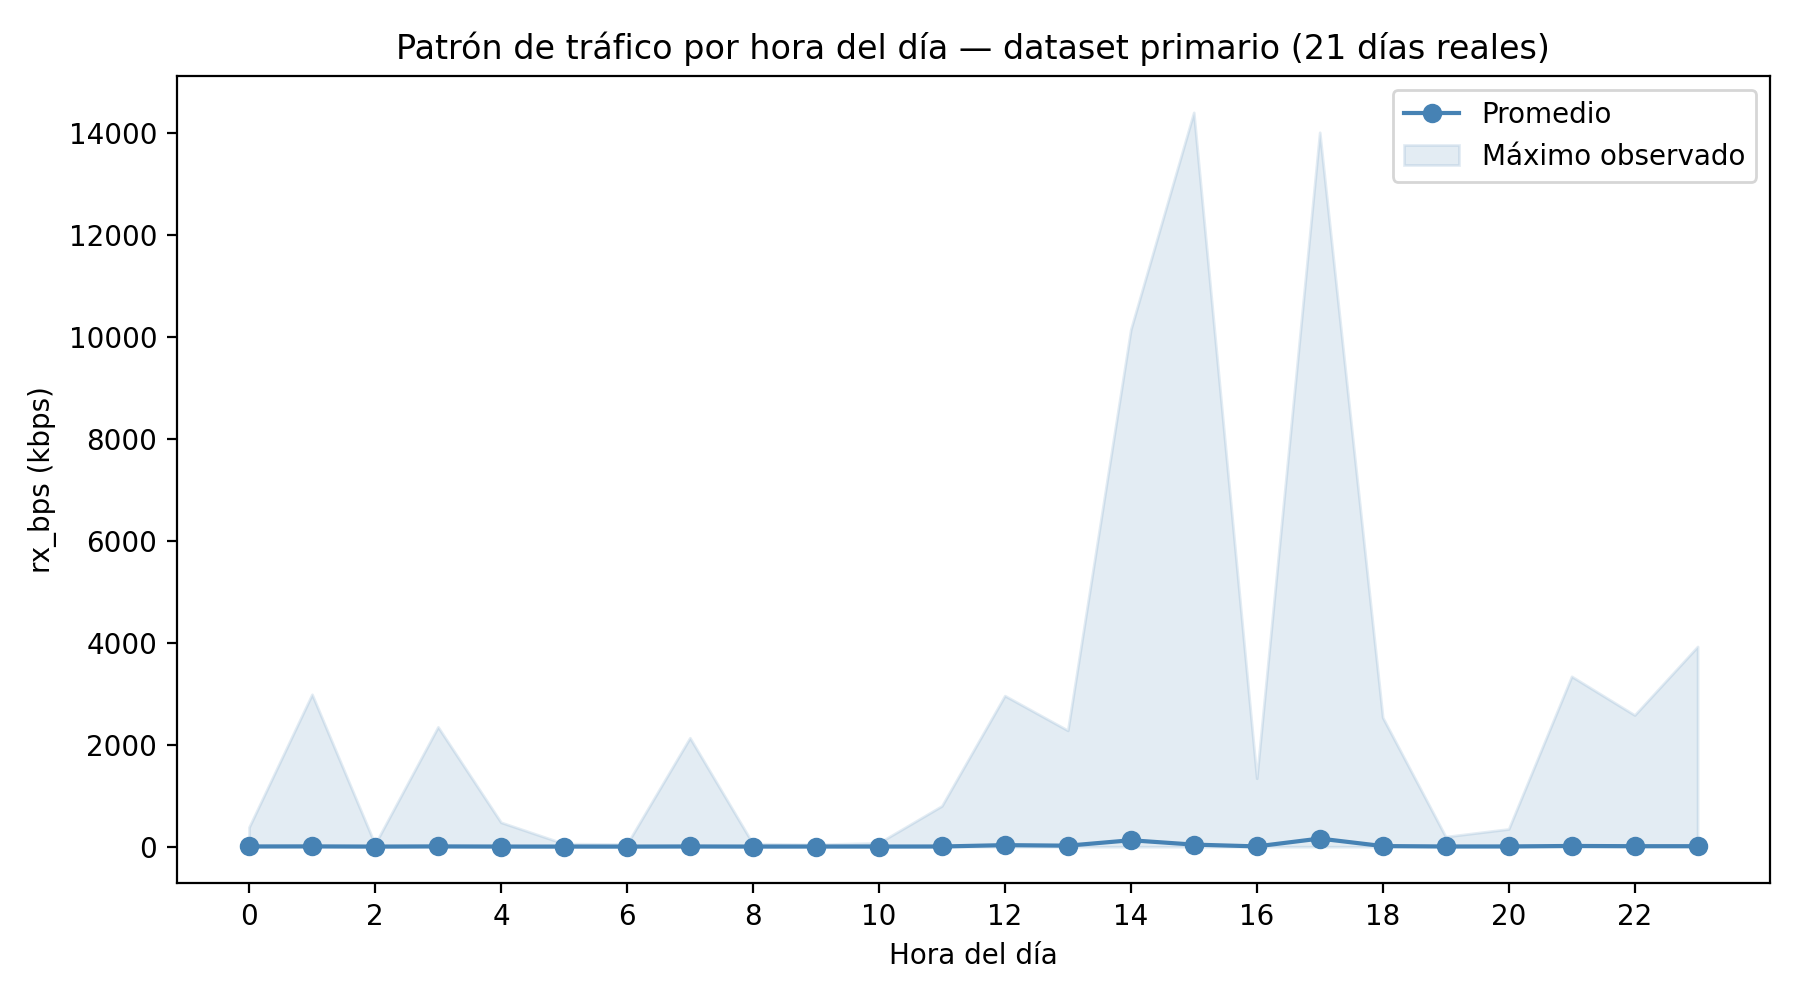
\includegraphics[width=0.8\textwidth]{patron_horario_real.png}
    \caption{Patrón de tráfico promedio y máximo por hora del día, \textit{dataset} primario.}
    \label{fig:patron_horario_real}
\end{figure}

\begin{figure}[H]
    \centering
    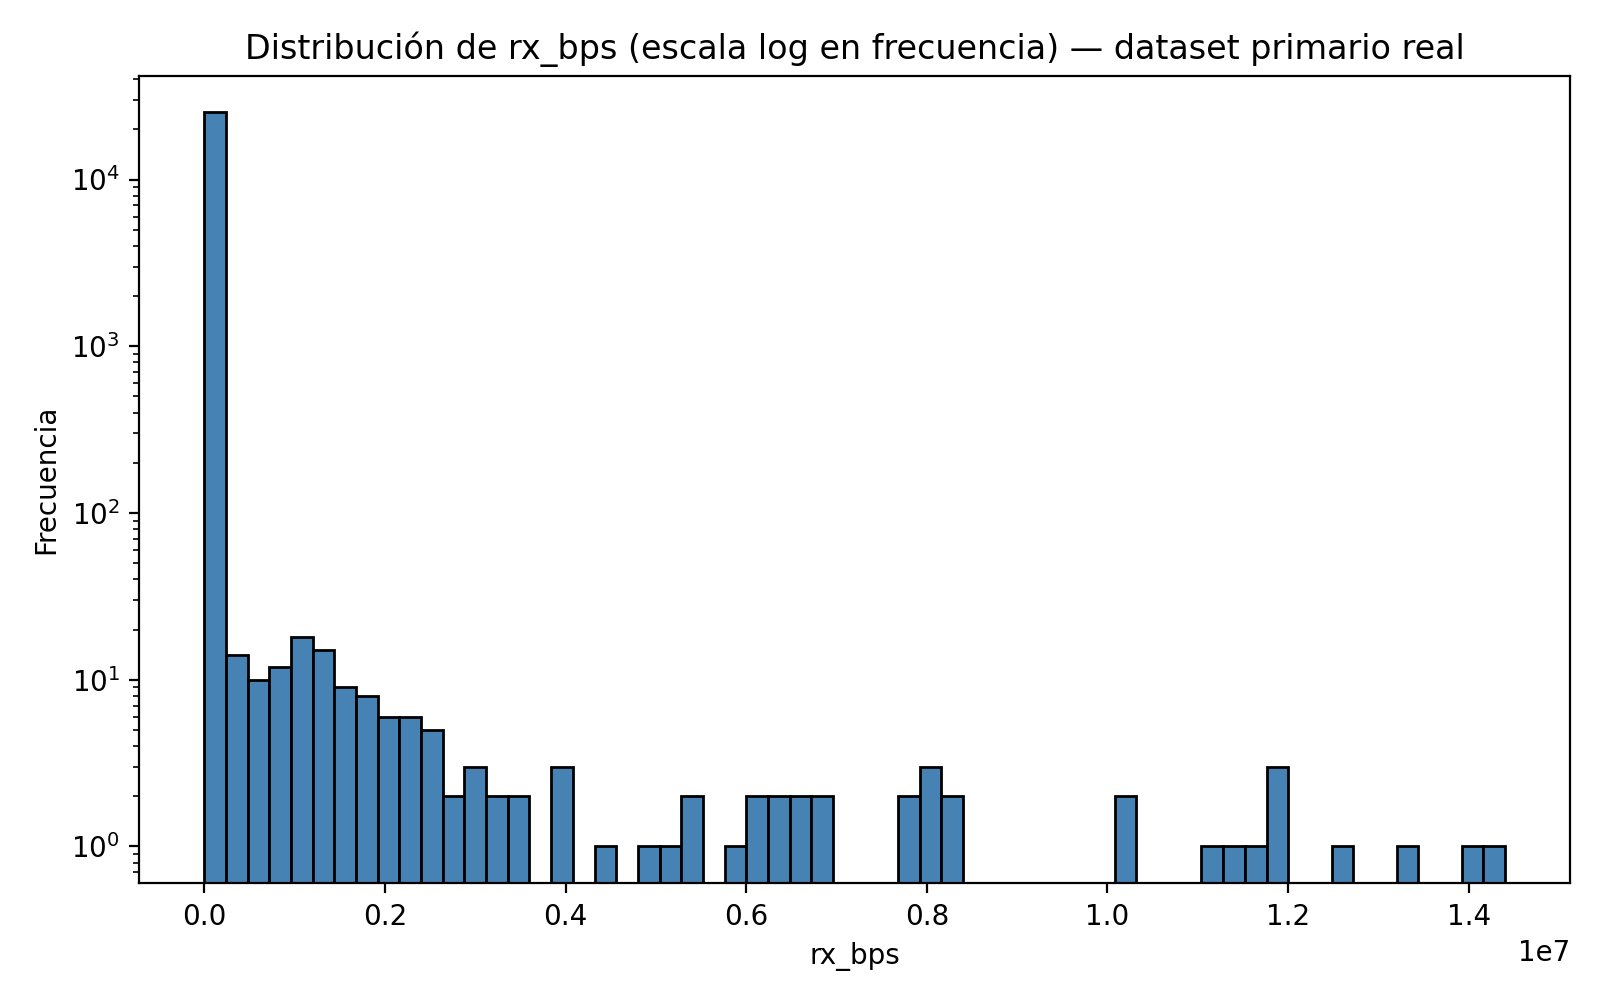
\includegraphics[width=0.75\textwidth]{histograma_real_log.png}
    \caption{Distribución de \texttt{rx\_bps} (escala logarítmica en frecuencia), \textit{dataset} primario.}
    \label{fig:histograma_real}
\end{figure}

\subsubsection*{Hallazgo: ausencia de congestión natural}

La utilización máxima fue de 1.44\,\% del ancho de banda contratado (1000 Mbps), frente a 32.3\,\% en el piloto MAWI, por lo que \textbf{no se observó ningún evento de congestión real} ($U \geq U_{th}=0.80$). Sin casos positivos no es posible entrenar ni evaluar la formulación de clasificación (Sección \ref{subsec:supervisado}), y la estabilidad del RTT indica que el comportamiento no lineal descrito por la Teoría de Colas no aparece en los datos reales. Consultado el comité asesor, se autorizó incorporar datos sintéticos como aumento de datos, con la condición de declarar siempre qué proporción de los datos es real y cuál sintética.

\subsection*{Generación de datos sintéticos calibrados}

Se generaron 37 días sintéticos, que junto con los 21 reales equivalen a los dos meses planificados originalmente (Sección \ref{sec:fuente_datos}). Su tráfico de fondo se calibró con un remuestreo \textit{bootstrap} de la distribución empírica por hora del día de los datos reales, lo que conserva sus ráfagas sin imponer una forma paramétrica.

Sobre ese fondo se inyectaron 126 eventos de congestión con perfil trapezoidal (ascenso, meseta y descenso) y varianza paramétrica. Duran entre 5 y 29 minutos (media de 17.4), cumpliendo la condición de sostenimiento de la Ecuación \ref{eq:congestion_instanciada}, y alcanzan una utilización pico entre 0.811 y 0.979 (media de 0.890) (Figura \ref{fig:distribucion_eventos}).

\begin{figure}[H]
    \centering
    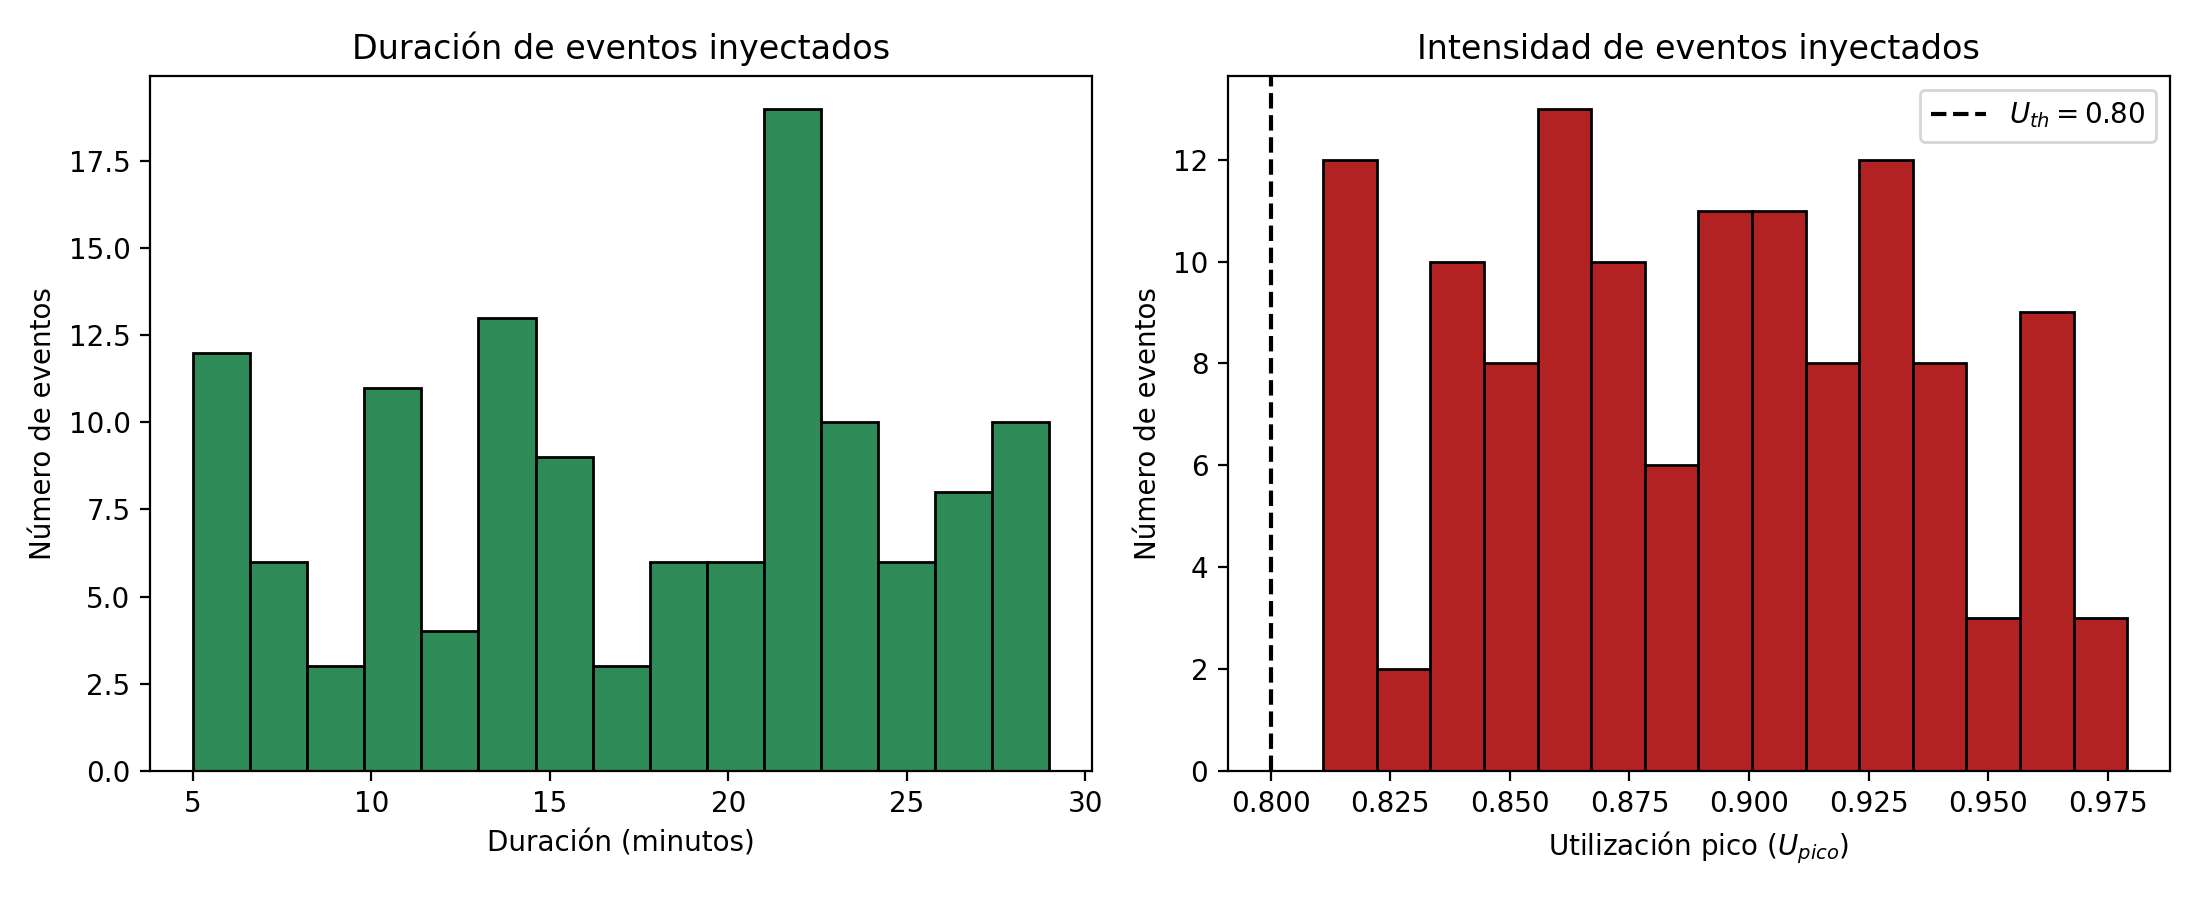
\includegraphics[width=\textwidth]{distribucion_eventos_sinteticos.png}
    \caption{Distribución de duración e intensidad de los 126 eventos de congestión sintéticos.}
    \label{fig:distribucion_eventos}
\end{figure}

El RTT y la pérdida de paquetes de estos eventos no se generaron con ruido aleatorio, sino que se derivaron de la utilización con el modelo de la Teoría de Colas (Sección \ref{sec:congestion}): el retraso en cola crece de forma asintótica (proporcional a $\frac{1}{1-\rho}$) y el descarte de paquetes se activa solo cuando $U \approx 0.85$. La Figura \ref{fig:ejemplo_evento} muestra un ejemplo: al cruzar $U=0.80$ en el minuto 10, el RTT y la pérdida se disparan.

\begin{figure}[H]
    \centering
    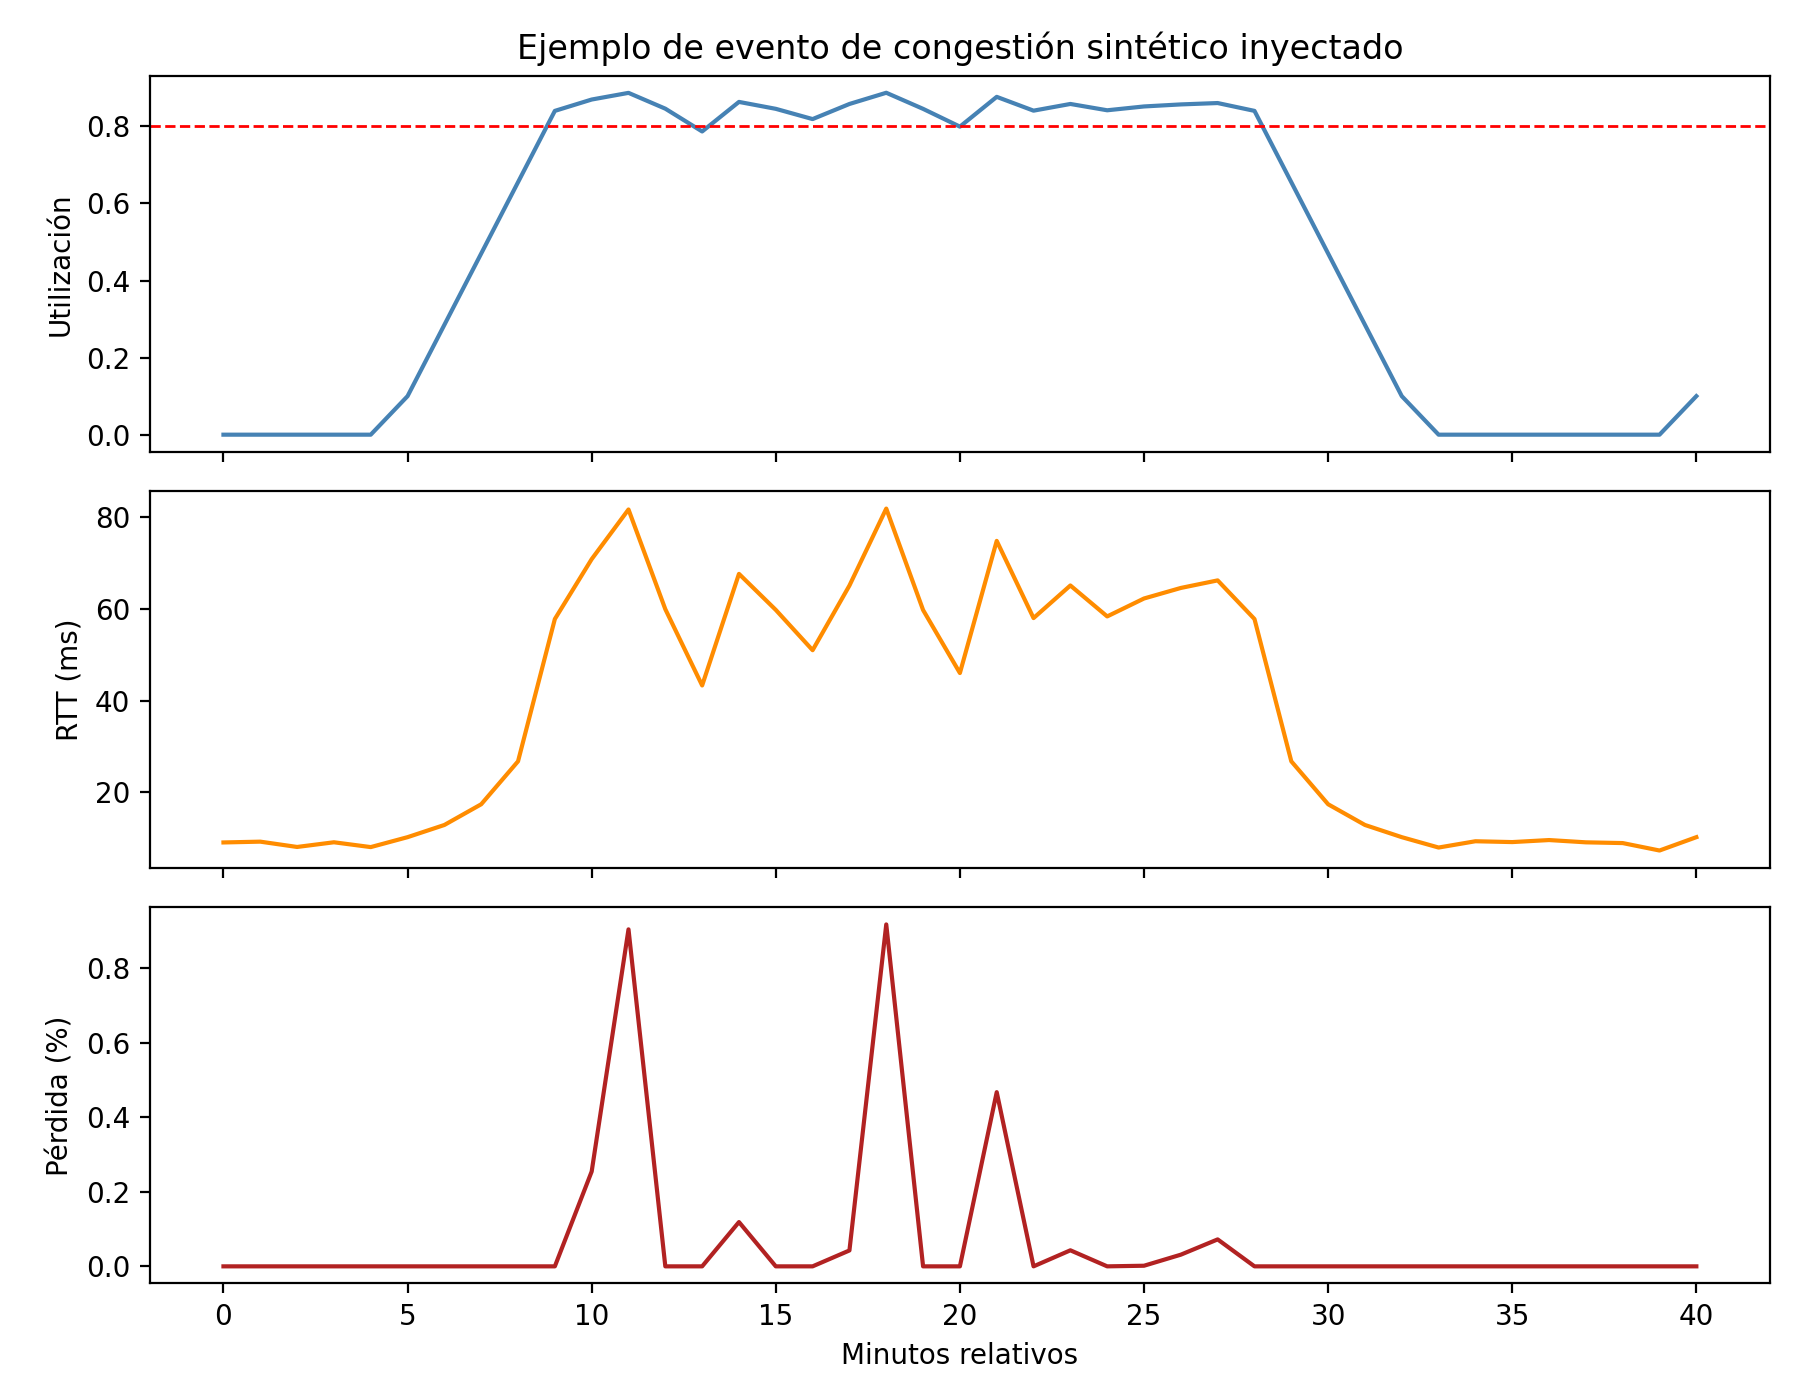
\includegraphics[width=0.85\textwidth]{ejemplo_evento_sintetico.png}
    \caption{Evento sintético inyectado: la utilización determina el RTT y la pérdida de paquetes según la Teoría de Colas.}
    \label{fig:ejemplo_evento}
\end{figure}

\subsection*{Diseño de evaluación: preservando la integridad de los datos reales}

Para que ningún resultado del Capítulo 6 provenga de una evaluación contaminada con datos sintéticos, se adoptó el siguiente diseño, verificado con comprobaciones automáticas en el código de procesamiento:

\begin{itemize}
    \item \textbf{Entrenamiento:} 60\,\% cronológico de los datos reales más 60\,\% de los sintéticos.
    \item \textbf{Regresión} (validación y prueba): solo el 20\,\%/20\,\% restante de los datos \textbf{reales}.
    \item \textbf{Clasificación} (validación y prueba): solo el 20\,\%/20\,\% restante de los datos \textbf{sintéticos}, pues la partición real no contiene, por construcción, ningún caso positivo.
\end{itemize}

\begin{table}[H]
    \centering
    \begin{tabular}{|l|l|l|r|r|}
        \hline
        \textbf{Conjunto} & \textbf{Propósito} & \textbf{Naturaleza} & \textbf{Filas} & \textbf{Casos de congestión} \\
        \hline
        Entrenamiento & Ambas tareas & Real + Sintético & 46\,872 & 993 (2.12\,\%) \\
        Val. regresión & Regresión & 100\,\% Real & 4\,914 & 0 \\
        Prueba regresión & Regresión & 100\,\% Real & 4\,949 & 0 \\
        Val. clasificación & Clasificación & 100\,\% Sintético & 10\,622 & 284 (2.67\,\%) \\
        Prueba clasificación & Clasificación & 100\,\% Sintético & 10\,622 & 275 (2.59\,\%) \\
        \hline
    \end{tabular}
    \caption{Composición final del \textit{dataset} primario tras la incorporación de datos sintéticos.}
    \label{tab:composicion_dataset_final}
\end{table}

Así, los resultados de regresión reflejan el comportamiento real de la red y los de clasificación, eventos sintéticos calibrados. Esta limitación se discute en la Sección 6.5 y se compensa parcialmente con la validación sobre MAWI reagregado a granularidad oficial (Sección \ref{sec:preprocesamiento}).

\subsection*{Extracción y decodificación de trazas de validación (MAWI)}

Se usaron trazas de tráfico troncal de 2026 del repositorio MAWI, distribuidas como capturas \texttt{.pcap.gz} con decenas de millones de paquetes por archivo. \texttt{tshark} resultó impráctico por su consumo de memoria al reconstruir flujos, así que se implementó un decodificador propio en Python que interpreta directamente el formato \textit{libpcap} sin decodificar el \textit{payload} y procesa en flujo (\textit{streaming}), agrupando los bytes en ventanas de 1 minuto, la misma del Capítulo 4. Como cada captura diaria dura solo 15 minutos, se procesó un lote secuencial de 120 trazas (30 horas efectivas) para obtener una serie suficientemente larga (Fragmento \ref{lst:parser_pcap}, Tabla \ref{tab:resumen_extraccion_mawi}).

\begin{lstlisting}[language=Python, caption={Extracto del decodificador de trazas libpcap en flujo.}, label={lst:parser_pcap}]
import struct

fmt_registro = "<IIII" # Formato struct (ts_sec, ts_usec, incl_len, orig_len)
ventana_seg = 60        # Agregacion a 1 minuto

while True:
    encabezado_paquete = f.read(16)
    if len(encabezado_paquete) < 16:
        break  # EOF

    ts_sec, ts_usec, incl_len, orig_len = struct.unpack(
        fmt_registro, encabezado_paquete
    )
    timestamp = ts_sec + (ts_usec / 1_000_000)
    ventana = int(timestamp // ventana_seg)
    acumulado[ventana] += orig_len

    # Salto rapido del payload sin saturar RAM
    f.seek(incl_len, 1) 
\end{lstlisting}

\begin{table}[H]
    \centering
    \begin{tabular}{|l|r|r|}
        \hline
        \textbf{Periodo procesado} & \textbf{Paquetes evaluados} & \textbf{Observaciones (1 min)} \\
        \hline
        Lote MAWI (120 trazas) & $\approx$ 21\,500\,000\,000 & 1\,800 \\
        \hline
    \end{tabular}
    \caption{Resultados de la extracción de telemetría sobre las trazas MAWI procesadas.}
    \label{tab:resumen_extraccion_mawi}
\end{table}

\subsection*{Exploración estadística preliminar}

Para probar el \textit{pipeline} antes de concluir la recolección primaria, se exploraron las 1\,800 observaciones de MAWI. La utilización se calculó con la definición de la Sección \ref{sec:congestion}, usando como ancho de banda nominal 11 Gbps, la suma de los dos enlaces monitoreados por \textit{samplepoint-F} desde julio de 2023 (1 Gbps hacia NTTC GIN y 10 Gbps hacia BBIX):

\begin{equation}
    U = \frac{\mbox{Throughput observado (bps)}}{11 \times 10^{9} \mbox{ bps}}
    \label{eq:utilizacion_instanciada_mawi}
\end{equation}

\begin{table}[H]
    \centering
    \begin{tabular}{|l|r|r|}
        \hline
        \textbf{Estadística} & \textbf{Throughput (Gbps)} & \textbf{Utilización ($U$)} \\
        \hline
        Mínimo & 0.19 & 0.017 \\
        Media & 1.71 & 0.155 \\
        Mediana & 1.66 & 0.151 \\
        Máximo & 3.55 & 0.323 \\
        Desviación estándar & 0.56 & 0.051 \\
        \hline
    \end{tabular}
    \caption{Estadísticas descriptivas del \textit{dataset} piloto MAWI (1\,800 observaciones, 1 minuto).}
    \label{tab:estadisticas_mawi_piloto}
\end{table}

La utilización máxima, de 32.3\,\%, nunca alcanza el umbral $U_{th}=0.80$ de la Ecuación \ref{eq:congestion_instanciada} (Figura \ref{fig:histograma_mawi}), lo que es coherente con una troncal académica sobredimensionada. Por ello, este subconjunto sirve para ejercitar el \textit{pipeline} en regresión (Sección \ref{subsec:supervisado}), pero no aporta positivos para clasificación. Solo durante la codificación y calibración se adoptó un umbral relativo de prueba ($U_{test} \geq 0.25$) para verificar la lógica de la matriz de confusión y de la métrica $TAE$, a la espera del umbral formal de 0.80 sobre el \textit{dataset} primario.

\begin{figure}[H]
    \centering
    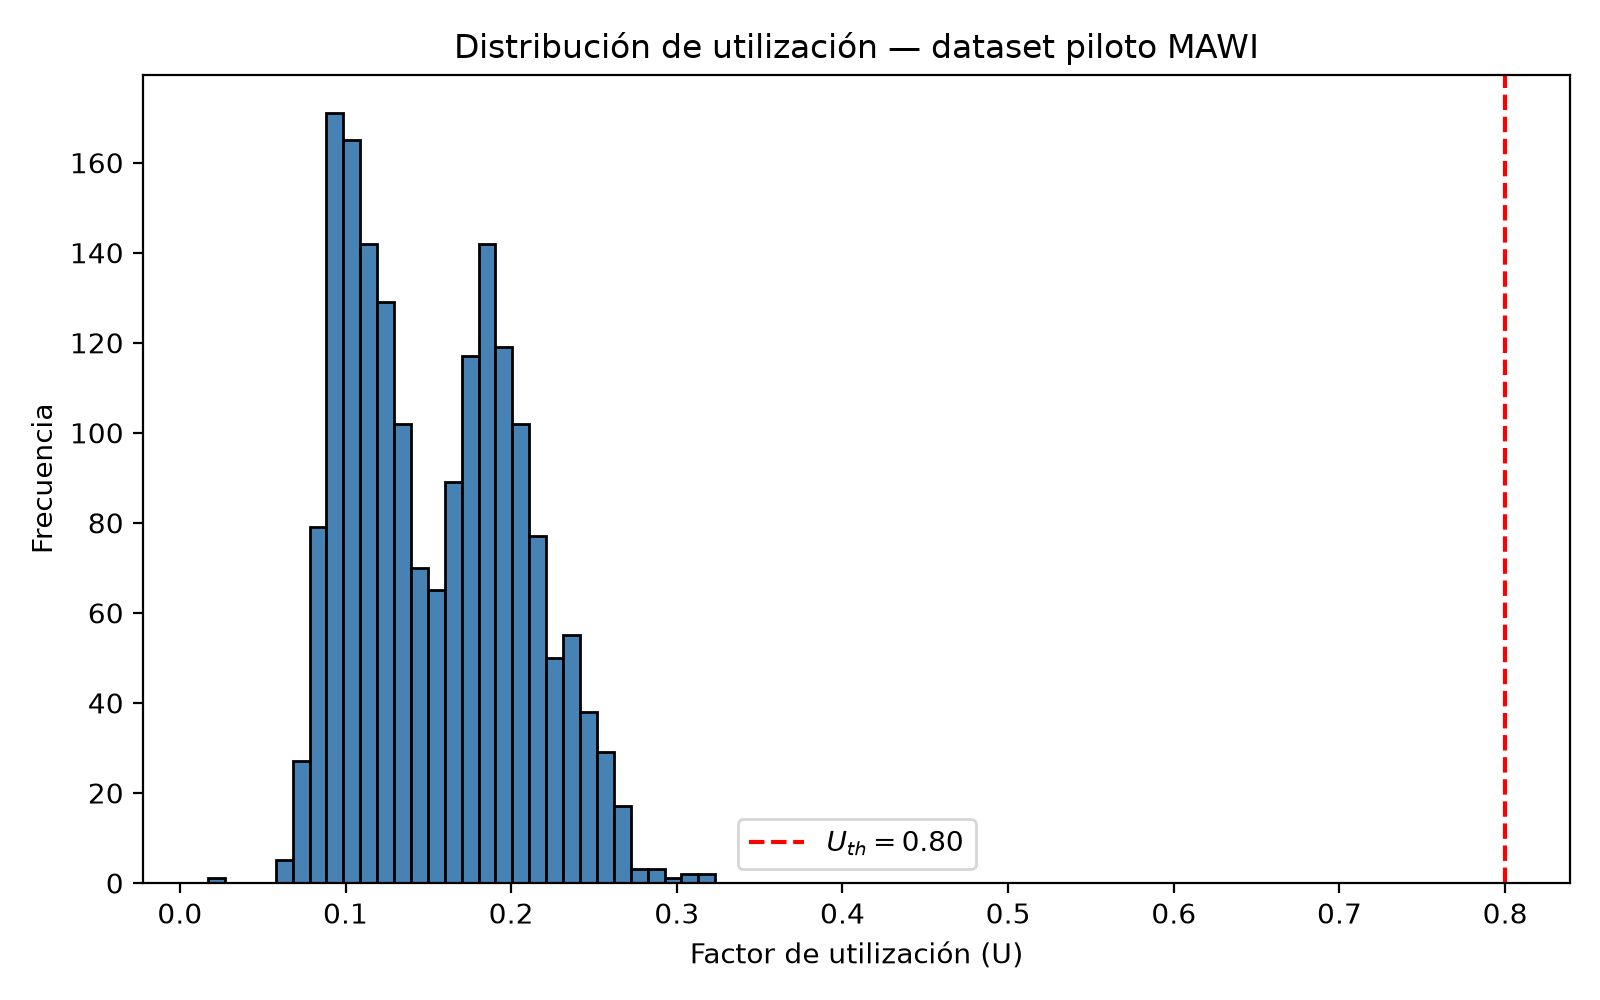
\includegraphics[width=0.75\textwidth]{histograma_utilizacion_mawi.png}
    \caption{Distribución del factor de utilización, \textit{dataset} piloto MAWI.}
    \label{fig:histograma_mawi}
\end{figure}

\section{Preprocesamiento}
\label{sec:preprocesamiento_desarrollo}

Esta etapa computacional tiene como objetivo transformar las series de tiempo crudas en las estructuras tensoriales requeridas por las bibliotecas de \textit{Machine Learning}. A continuación, se documenta la ejecución de este \textit{pipeline} en dos fases: primero, la calibración algorítmica sobre el \textit{dataset} piloto MAWI; y segundo, la 
aplicación del preprocesamiento con los parámetros oficiales sobre el \textit{dataset} primario híbrido (real y sintético).

\subsection*{Fase 1: Calibración del \textit{pipeline} sobre el \textit{dataset} piloto MAWI}

Sobre el conjunto de 1\,800 observaciones a granularidad de 1 minuto descrito en la Sección \ref{sec:obtencion_exploracion}, se aplicaron inicialmente las etapas de preprocesamiento establecidas en el Capítulo 4 para validar la lógica del código.

\subsubsection*{Limpieza y manejo de discontinuidades}

Dado que el \textit{dataset} piloto se construyó mediante la concatenación secuencial de un lote de 120 trazas individuales de 15 minutos, las fronteras entre archivos introdujeron discontinuidades temporales. Para garantizar la integridad de los algoritmos autorregresivos, la limpieza se ejecutó empleando las estructuras de datos bidimensionales 
(\texttt{DataFrame}) de la biblioteca \texttt{pandas}. Se aplicaron rutinas de interpolación lineal (\texttt{.interpolate(method='linear', limit=2)}) para imputar micro-cortes internos, seguidas de la eliminación de observaciones residuales no válidas (\texttt{.dropna()}) en los bordes de concatenación. Este proceso de purga redujo el conjunto de 
datos de 1\,800 a un total efectivo de $n=1\,774$ observaciones continuas y estructuradas.

\subsubsection*{División cronológica y escalado sin fuga de datos}

La división cronológica se programó como una partición dura de la serie ordenada temporalmente $\{x_1, x_2, \dots, x_n\}$ en tres segmentos contiguos y no traslapados:

\begin{equation}
\begin{aligned}
    \text{Entrenamiento} &= \{x_1, \dots, x_{\lfloor 0.6n \rfloor}\}, \\
    \text{Validación} &= \{x_{\lfloor 0.6n \rfloor + 1}, \dots, x_{\lfloor 0.8n \rfloor}\}, \\
    \text{Prueba} &= \{x_{\lfloor 0.8n \rfloor + 1}, \dots, x_n\}
\end{aligned}
\label{eq:split_cronologico}
\end{equation}

Para el \textit{dataset} piloto, con $n=1\,774$, la indexación generó $1\,064$ observaciones de entrenamiento, $355$ de validación y $355$ de prueba, proporciones consistentes con el diseño metodológico (Tabla \ref{tab:split_mawi_piloto}).

\begin{table}[H]
    \centering
    \begin{tabular}{|l|r|r|}
        \hline
        \textbf{Conjunto} & \textbf{Observaciones} & \textbf{Proporción} \\
        \hline
        Entrenamiento & 1\,064 & 60.0\,\% \\
        Validación & 355 & 20.0\,\% \\
        Prueba & 355 & 20.0\,\% \\
        \hline
    \end{tabular}
    \caption{Composición de la división cronológica del \textit{dataset} piloto MAWI tras el preprocesamiento.}
    \label{tab:split_mawi_piloto}
\end{table}

Posterior a la partición, se aplicó la normalización Min-Max (Ecuación \ref{eq:minmax}). Desde la perspectiva de ingeniería de \textit{software}, para prevenir el antipatrón de fuga de datos (\textit{data leakage}), este escalado se implementó utilizando la clase \texttt{MinMaxScaler} de \texttt{scikit-learn}. Se garantizó por diseño que el método 
\texttt{fit\_transform()} se ejecutara de manera exclusiva sobre el conjunto de entrenamiento, mientras que a los conjuntos de validación y prueba se les aplicó únicamente el método \texttt{transform()}, forzándolos a mapearse bajo la distribución matemática descubierta en el pasado, sin contaminar el modelo con conocimiento futuro. Para la variable 
de utilización, la ecuación instanciada operó de la siguiente forma:

\begin{equation}
    U_{\mbox{\scriptsize norm}} = \frac{U - 0.017045}{0.323168 - 0.017045}
    \label{eq:minmax_instanciada_mawi}
\end{equation}

\subsubsection*{Ventaneo secuencial y conformación de tensores}

Para habilitar el aprendizaje de la arquitectura recurrente LSTM, se implementó una función propia de ventana deslizante (\textit{Sliding Window}) mediante la manipulación de arreglos de \texttt{NumPy}. Dado el volumen del piloto, se configuró provisionalmente una ventana de observación $w=15$ minutos y un horizonte de predicción $h=5$ minutos. 
La conformación lógica de cada par de entrada/salida se instanció como:

\begin{equation}
    X_t = \left[U(t-15), \dots, U(t-1)\right] \longrightarrow y_t = U(t+5)
    \label{eq:ventaneo_instanciada_mawi}
\end{equation}

El resultado es la redimensión de los datos en un tensor tridimensional con la forma \texttt{(muestras, pasos\_de\_tiempo, caracteristicas)}, requisito ineludible para la capa de entrada (\textit{Input Layer}) del \textit{framework} \texttt{Keras/TensorFlow}. Este proceso generó 1\,044 secuencias para entrenamiento, 335 para validación y 335 para prueba.

\subsection*{Fase 2: Ejecución oficial sobre el \textit{dataset} primario}

Una vez validado el código, el preprocesamiento se aplicó sobre el \textit{dataset} primario (datos reales y sintéticos), introduciendo los parámetros oficiales y el manejo de sesiones exigido por las interrupciones operativas.

\subsubsection*{Detección de sesiones continuas}

El \textit{dataset} primario presenta dos fuentes de discontinuidad temporal: las interrupciones de conectividad VPN reales y la frontera cronológica entre los datos reales y los sintéticos inyectados. Aplicando un criterio de segmentación estricto (cortes superiores a 5 minutos), se identificaron 10 sesiones dentro del conjunto de entrenamiento 
(Tabla \ref{tab:sesiones_train}).

\begin{table}[H]
    \centering
    \small
    \begin{tabular}{|r|r|l|l|l|}
        \hline
        \textbf{Sesión} & \textbf{Filas} & \textbf{Naturaleza} & \textbf{Inicio} & \textbf{Fin} \\
        \hline
        10 & 31\,934 & Sintética & 2026-09-20 00:29 & 2026-10-12 04:42 \\
        0  & 6\,137  & Real & 2026-08-29 17:30 & 2026-09-02 23:50 \\
        5  & 1\,401  & Real & 2026-09-07 00:29 & 2026-09-07 23:49 \\
        2  & 1\,401  & Real & 2026-09-04 00:29 & 2026-09-04 23:49 \\
        4  & 1\,401  & Real & 2026-09-06 00:29 & 2026-09-06 23:49 \\
        3  & 1\,401  & Real & 2026-09-05 00:29 & 2026-09-05 23:49 \\
        7  & 1\,401  & Real & 2026-09-10 00:29 & 2026-09-10 23:49 \\
        9  & 658    & Real & 2026-09-12 00:29 & 2026-09-12 11:26 \\
        6  & 611    & Real & 2026-09-09 13:39 & 2026-09-09 23:49 \\
        1  & 527    & Real & 2026-09-03 15:03 & 2026-09-03 23:49 \\
        \hline
    \end{tabular}
    \caption{Sesiones continuas detectadas en el conjunto de entrenamiento del \textit{dataset} primario.}
    \label{tab:sesiones_train}
\end{table}

Esta segmentación resulta indispensable para calcular las variables de rezago, evitando que el algoritmo tome datos de una sesión distinta a través de un "salto en el tiempo". Sobre cada una de estas 10 sesiones se aplicó independientemente la interpolación lineal de huecos cortos (con el límite flexibilizado de 6 muestras, justificado en la Sección 
\ref{sec:obtencion_exploracion}). Tras la limpieza y eliminación de observaciones incompletas en los bordes, el conjunto de entrenamiento quedó compuesto por 46\,872 observaciones.

\subsubsection*{Normalización sin fuga de datos entre las cinco particiones}
A diferencia del piloto, el diseño de evaluación dual establecido requiere que la normalización Min-Max se aplique de forma estructurada sobre \textbf{cinco} particiones (entrenamiento unificado, y pares de validación/prueba separados para regresión y clasificación). Para prevenir estrictamente la fuga de información temporal (\textit{data leakage}), los parámetros de escalamiento escalar (mínimo y máximo) se calcularon de manera exclusiva sobre la matriz de entrenamiento y se proyectaron, sin recálculo alguno, sobre las cuatro particiones de evaluación restantes.

La Figura \ref{fig:comparativa_distribuciones} expone la matriz de histogramas resultante de este proceso, ofreciendo una comprobación visual crítica de la asimetría del diseño experimental. La fila superior (paneles en gris) ilustra las particiones dominadas por el tráfico de fondo: mientras que el conjunto de entrenamiento (panel superior izquierdo) abarca todo el espectro [0, 1] debido a la inyección de anomalías, las particiones de regresión (100\,\% reales, paneles superior central y derecho) colapsan su densidad de probabilidad íntegramente hacia el extremo izquierdo, confirmando que la red operó muy por debajo del umbral de congestión $U_{th}=0.80$ (línea roja discontinua). En contraste, la fila inferior (paneles en naranja) corrobora la idoneidad de los conjuntos de clasificación (100\,\% sintéticos): aquí se aprecia cómo la masa anómala inyectada franquea exitosamente el umbral, dotando matemáticamente a la evaluación de los eventos necesarios para probar la capacidad de detección.

\begin{figure}[H]
    \centering
    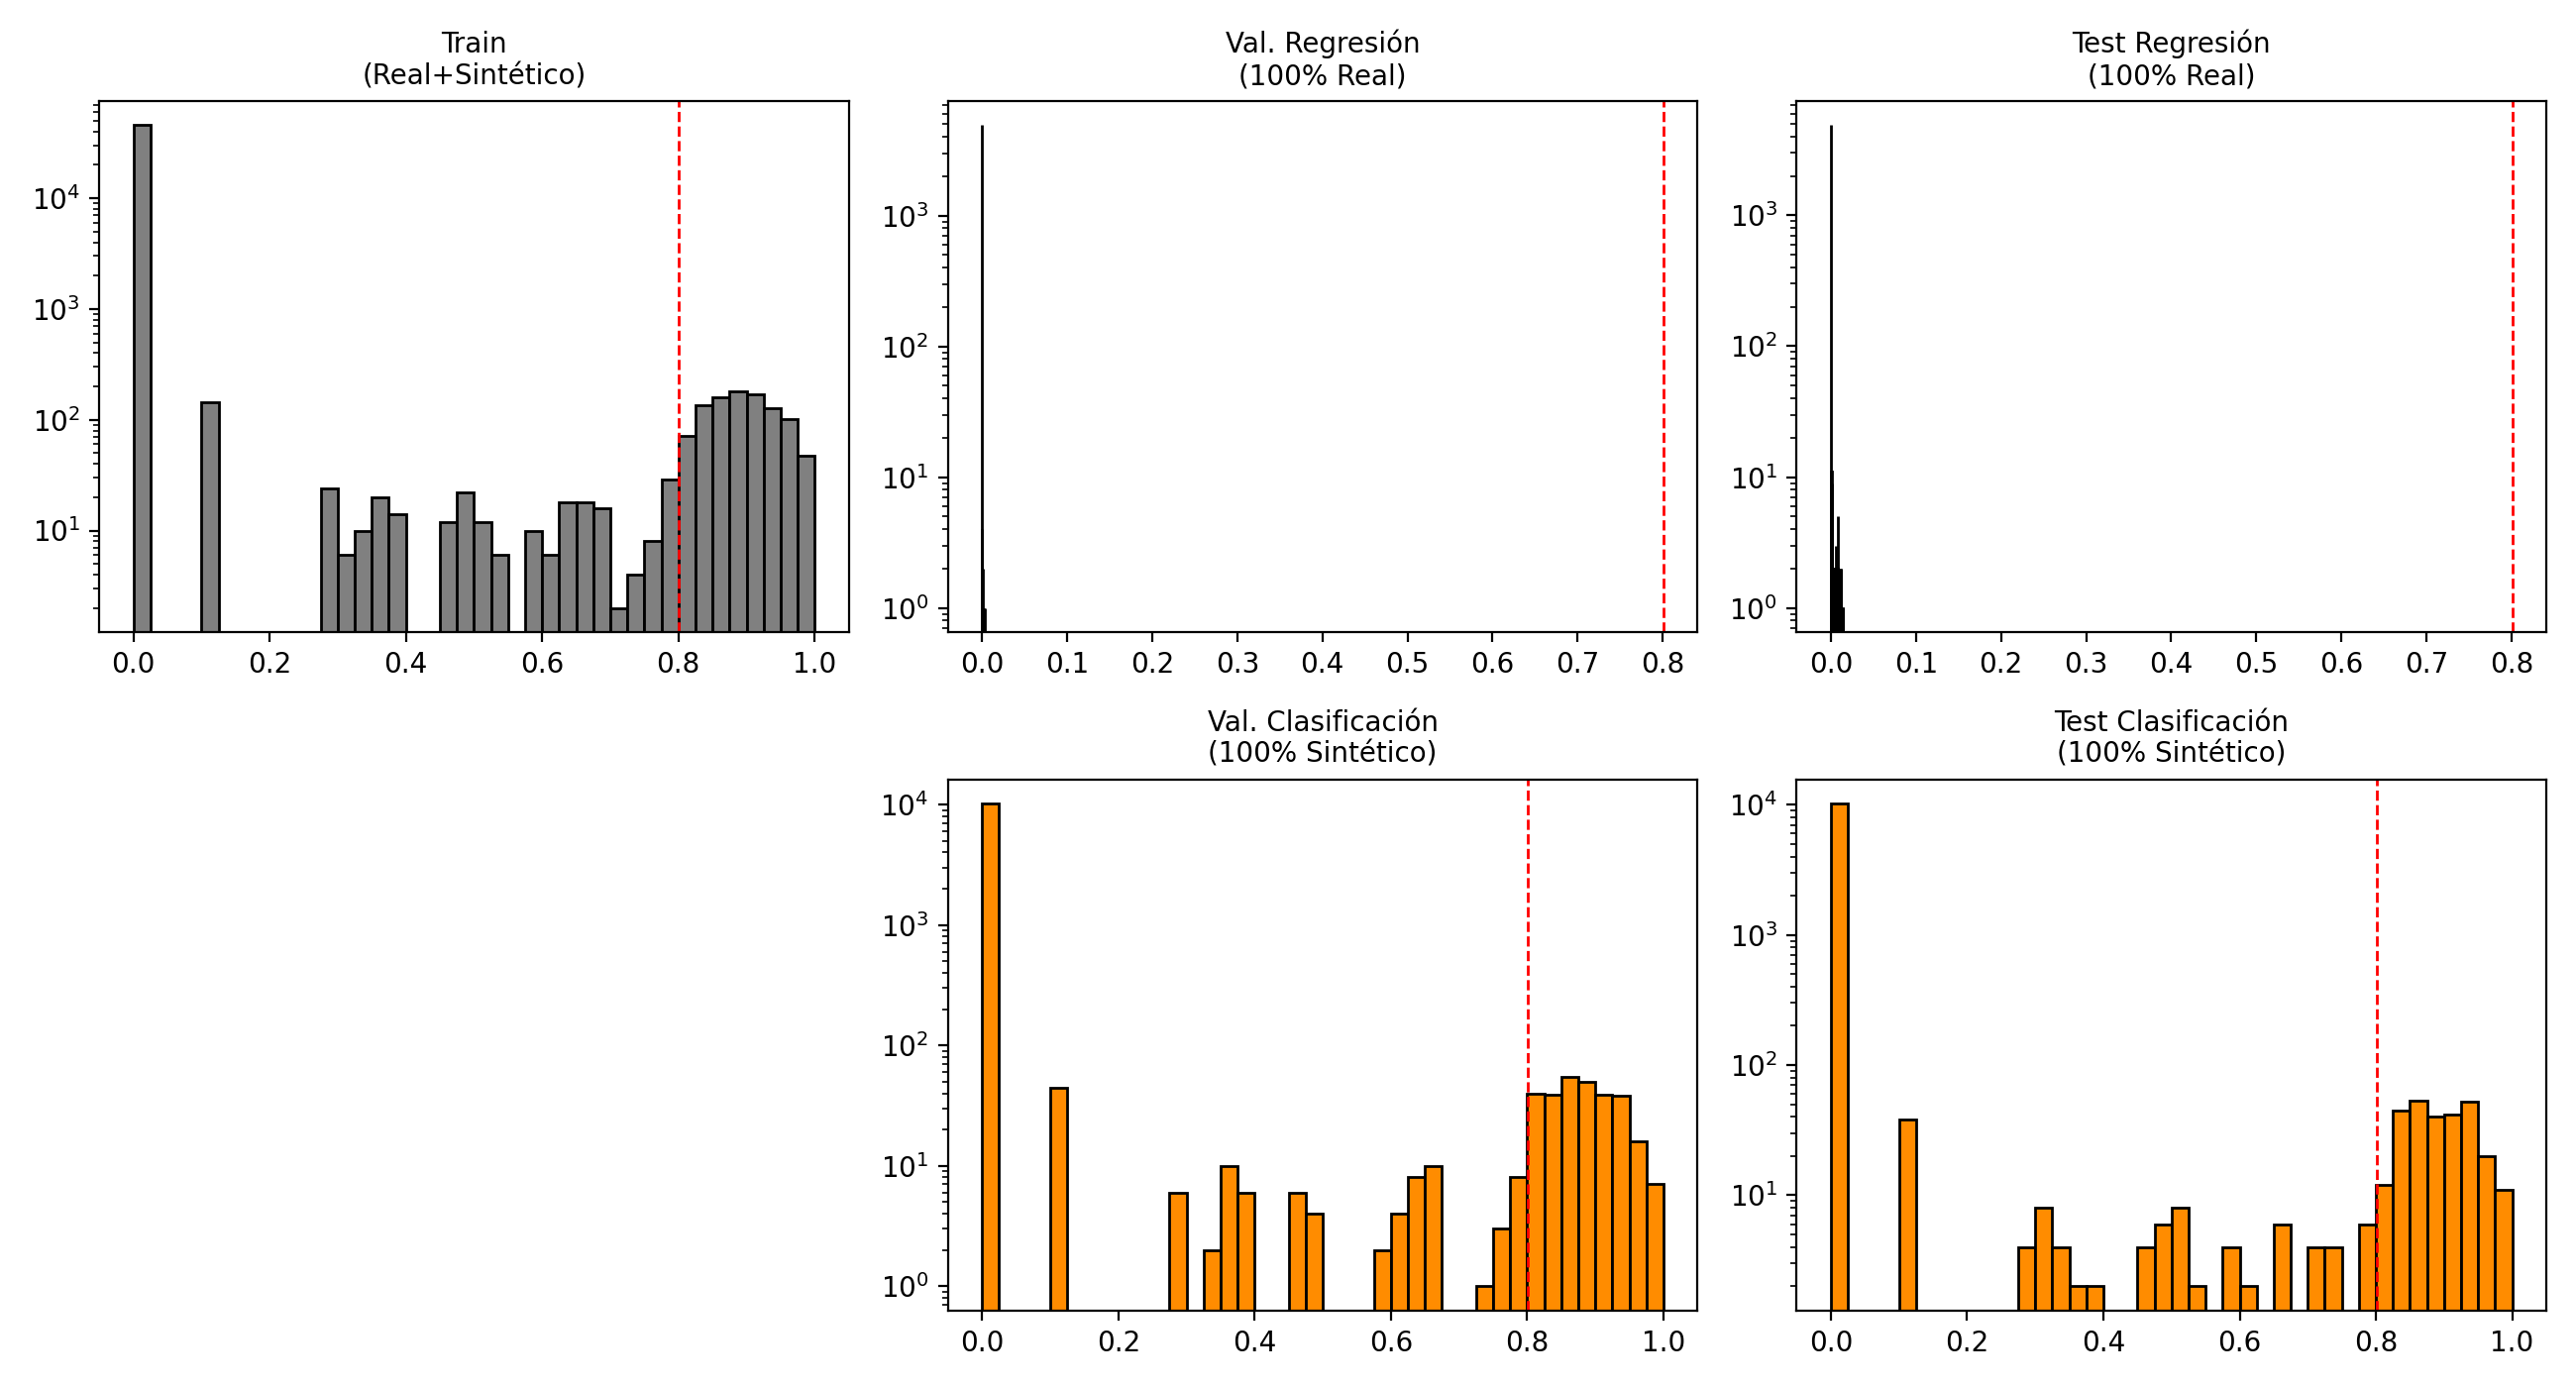
\includegraphics[width=\textwidth]{comparativa_distribuciones_conjuntos.png}
    \caption{Matriz de distribución de utilización normalizada: contraste entre el espectro del entrenamiento (arriba izq.), la contención del tráfico real (arriba centro/der.) y la masa anómala inyectada (abajo).}
    \label{fig:comparativa_distribuciones}
\end{figure}

La Tabla \ref{tab:rangos_normalizados} resume los rangos topológicos resultantes. Es imperativo señalar que la existencia de máximos ínfimos en las particiones de regresión (apenas 0.0144) o de mínimos fraccionalmente negativos no constituye un error de procesamiento, sino la consecuencia analítica directa y deseada de haber congelado los escalares en el conjunto de entrenamiento, garantizando así una evaluación completamente ciega a magnitudes no observadas en el pasado.

\begin{table}[H]
    \centering
    \begin{tabular}{|l|r|r|r|}
        \hline
        \textbf{Conjunto} & \textbf{Mínimo} & \textbf{Máximo} & \textbf{Observaciones} \\
        \hline
        Entrenamiento & 0.000000 & 1.000000 & 46\,872 \\
        Validación (regresión) & 0.0000001 & 0.002992 & 4\,914 \\
        Prueba (regresión) & 0.0000001 & 0.014414 & 4\,949 \\
        Validación (clasificación) & $-$0.0000001 & 1.000000 & 10\,622 \\
        Prueba (clasificación) & $-$0.0000001 & 1.000000 & 10\,622 \\
        \hline
    \end{tabular}
    \caption{Rango de utilización normalizada por partición, \textit{dataset} primario. Los valores atípicos certifican la ausencia de fuga de información metodológica.}
    \label{tab:rangos_normalizados}
\end{table}
\newpage

\subsubsection*{Ventaneo secuencial oficial}

Finalmente, se aplicó la granularidad y los parámetros \textbf{oficiales} establecidos en el Capítulo 4 para el \textit{dataset} primario: ventana de observación $w=30$ minutos y horizonte de predicción $h=5$ minutos. La variable objetivo de clasificación se definió como una variable binaria $\mathbb{1}[U(t+h) \geq U_{th}]$.

\begin{equation}
    X_t = \left[U(t-30), \dots, U(t-1)\right] \longrightarrow y_t = U(t+5)
    \label{eq:ventaneo_instanciada_primario}
\end{equation}

El proceso, respetando las fronteras de sesión, generó 46\,582 secuencias de entrenamiento, 4\,796 y 4\,833 secuencias para validación y prueba de regresión respectivamente, y 10\,593 secuencias para cada partición de clasificación, dejando los tensores listos para el entrenamiento de los modelos predictivos documentados a continuación.

\section{Construcción del modelo ARIMA}
\label{sec:arima_desarrollo}

Conforme a la Sección \ref{sec:modelos_justificacion}, ARIMA se implementó con \texttt{statsmodels} como línea base estadística. El procedimiento fue el mismo en ambos conjuntos de datos: primero se calibró sobre el piloto MAWI y después se aplicó al \textit{dataset} primario.

\subsection*{Identificación del orden}

Para fijar el orden de diferenciación $d$ se aplicó la prueba de Dickey-Fuller Aumentada (\texttt{stattools.adfuller}) sobre la serie de utilización del conjunto de entrenamiento: si no se rechazaba la no estacionariedad ($p>0.05$), la serie se diferenciaba (Sección \ref{subsec:arima}). Luego se evaluaron las dieciséis combinaciones $(p,d,q)$ con $p,q \in \{0,1,2,3\}$ y se seleccionó la de menor Criterio de Información de Akaike (AIC). En MAWI la serie requirió $d=1$ y el orden seleccionado fue ARIMA(1,1,1). En el \textit{dataset} primario, el modelo se ajustó sobre la sesión sintética continua más larga del conjunto de entrenamiento (31\,934 observaciones, Tabla \ref{tab:sesiones_train}), que contiene tanto el régimen normal como los 126 eventos de congestión inyectados. La serie resultó estacionaria ($d=0$) y se seleccionó ARIMA(3,0,3). Los estadísticos de la prueba, la búsqueda por AIC, los coeficientes y el diagnóstico de residuos se reportan en el Capítulo \ref{cap:resultados}.

\subsection*{Esquema de evaluación}

Para regresión se empleó pronóstico progresivo (\textit{walk-forward validation}) con horizonte $h=5$: en cada instante $t$ se predice el valor en $t+h$ y, a continuación, el valor real observado se incorpora al modelo antes de la siguiente predicción, emulando un despliegue en tiempo real. En el \textit{dataset} primario la evaluación se hizo por bloques (Sección \ref{sec:evaluacion}) y solo sobre las particiones reales de validación y prueba (Sección \ref{sec:obtencion_exploracion}). Se omitió el MAPE porque la utilización real cercana a cero hace inestable su denominador (Sección \ref{sec:evaluacion}).

Para clasificación, las predicciones continuas se binarizaron con el umbral de prueba $U_{test} \geq 0.25$ en MAWI y con $U_{th}=0.80$ en el \textit{dataset} primario, este último sobre las particiones sintéticas aisladas. Una alerta cuenta como verdadero positivo solo si la predicción supera el umbral antes del evento real. Las métricas de clasificación y el $TAE$ se calcularon según la Sección \ref{sec:evaluacion}, y los resultados de ambas tareas se presentan en el Capítulo \ref{cap:resultados}.

\begin{table}[H]
    \centering
    \begin{tabular}{|l|p{5.5cm}|}
        \hline
        \textbf{Parámetro} & \textbf{Configuración} \\
        \hline
        Biblioteca & \texttt{statsmodels} \\
        Orden de diferenciación $d$ & Prueba ADF ($\alpha=0.05$) \\
        Búsqueda de $(p,q)$ & $p,q \in \{0,1,2,3\}$ (16 combinaciones) \\
        Criterio de selección & Mínimo AIC \\
        Horizonte $h$ & 5 pasos \\
        Evaluación de regresión & Pronóstico progresivo por bloques \\
        Umbral de clasificación & $U_{test}=0.25$ (MAWI); $U_{th}=0.80$ (primario) \\
        \hline
    \end{tabular}
    \caption{Configuración del modelo ARIMA.}
    \label{tab:config_arima}
\end{table}

\section{Construcción del modelo \textit{Random Forest}}
\label{sec:rf_desarrollo}

Conforme a la Sección \ref{sec:modelos_justificacion}, se implementó \textit{Random Forest} como representante del \textit{Machine Learning} clásico con \texttt{RandomForestRegressor} y su contraparte \texttt{RandomForestClassifier} de \texttt{scikit-learn}. Como en ARIMA, el modelo se calibró primero sobre MAWI y luego se reentrenó sobre el \textit{dataset} primario con los mismos hiperparámetros, usando sus 46\,872 observaciones de entrenamiento (Sección \ref{sec:obtencion_exploracion}).

\subsection*{Preparación de las entradas}

El tensor tridimensional del preprocesamiento (Sección \ref{sec:preprocesamiento_desarrollo}) se aplanó a la entrada tabular que requieren los algoritmos clásicos. Cada observación se representa con cinco rezagos ($U_{\mbox{\scriptsize lag1}}$ a $U_{\mbox{\scriptsize lag5}}$) y la media de la ventana ($U_{\mbox{\scriptsize media\_movil}}$) como característica explícita. A diferencia de ARIMA, que opera sobre su propia serie y sus residuos, el ensamble mapea de forma no lineal todo el vector de entrada contra el objetivo. La utilización se escaló con Min-Max, por lo que sus métricas se reportan en escala normalizada, a diferencia de ARIMA, que se mantuvo en escala original.

\subsection*{Configuración y esquema de evaluación}

La Tabla \ref{tab:config_rf} resume la configuración, idéntica en ambos conjuntos de datos.

\begin{table}[H]
    \centering
    \begin{tabular}{|l|p{6cm}|}
        \hline
        \textbf{Parámetro} & \textbf{Configuración} \\
        \hline
        Biblioteca & \texttt{scikit-learn} \\
        Número de árboles & 200 \\
        Profundidad máxima & 10 (\texttt{max\_depth=10}) \\
        Entradas & 5 rezagos y media móvil de la ventana \\
        Escalado & Min-Max \\
        Evaluación de regresión & Particiones de validación y prueba (reales en el primario) \\
        Umbral de clasificación & $U_{test}=0.25$ (MAWI); $U_{th}=0.80$ (primario) \\
        Importancia de variables & Disminución media de impureza \\
        \hline
    \end{tabular}
    \caption{Configuración del modelo \textit{Random Forest}.}
    \label{tab:config_rf}
\end{table}

La evaluación sigue el diseño de la Sección \ref{sec:obtencion_exploracion}: la regresión se evalúa sobre las particiones reales y la clasificación, sobre las sintéticas aisladas, binarizando las predicciones con el umbral correspondiente a cada conjunto de datos. La importancia de las variables se calculó a partir de la disminución media de impureza que aporta cada entrada en los árboles. Los resultados de ambas tareas se presentan en la Sección \ref{cap:resultados}.

\section{Construcción del modelo LSTM}
\label{sec:lstm_desarrollo}

Conforme a la Sección \ref{sec:modelos_justificacion}, se implementó una red LSTM como representante del \textit{Deep Learning} con \texttt{Keras/TensorFlow}. A diferencia de \textit{Random Forest}, la red consume directamente los tensores tridimensionales de la ventana deslizante (Sección \ref{sec:preprocesamiento_desarrollo}), sin aplanarlos, para aprovechar el orden temporal de la secuencia. Como en los modelos anteriores, se calibró primero sobre MAWI y luego se reentrenó sobre el \textit{dataset} primario con la misma arquitectura y el mismo criterio de parada, usando sus 46\,582 secuencias de entrenamiento.

\subsection*{Arquitectura y entrenamiento}

La red es secuencial: una capa LSTM de 32 unidades con activación tangente hiperbólica, una capa densa de 16 unidades con ReLU y una neurona de salida lineal para la regresión de la utilización, con 4\,897 parámetros entrenables. Se minimizó el MSE con Adam y lotes de 16 secuencias, durante un máximo de 100 épocas. Como regularización se usó detención temprana (\textit{Early Stopping}) sobre la pérdida de validación, con paciencia de 10 épocas y restauración de los mejores pesos. En el \textit{dataset} primario, esa partición de validación es la de regresión, es decir, 100\,\% tráfico real (Sección \ref{sec:obtencion_exploracion}). La Tabla \ref{tab:config_lstm} resume la configuración.

\begin{table}[H]
    \centering
    \begin{tabular}{|l|p{6cm}|}
        \hline
        \textbf{Parámetro} & \textbf{Configuración} \\
        \hline
        Biblioteca & \texttt{Keras/TensorFlow} \\
        Capas & LSTM (32, tanh), Dense (16, ReLU), Dense (1, lineal) \\
        Parámetros entrenables & 4\,897 \\
        Entrada & Tensor 3D de la ventana deslizante \\
        Función de pérdida y optimizador & MSE, Adam \\
        Tamaño de lote & 16 \\
        Épocas máximas & 100 \\
        Detención temprana & Paciencia de 10 épocas; restauración de mejores pesos \\
        Escalado & Min-Max \\
        Umbral de clasificación & $U_{test}=0.25$ (MAWI); $U_{th}=0.80$ (primario) \\
        \hline
    \end{tabular}
    \caption{Configuración del modelo LSTM.}
    \label{tab:config_lstm}
\end{table}

\subsection*{Esquema de evaluación}

La evaluación sigue el diseño de la Sección \ref{sec:obtencion_exploracion}: la regresión se mide sobre las particiones reales y la clasificación, sobre las sintéticas aisladas, binarizando la salida continua con el umbral de cada conjunto de datos. Las curvas de aprendizaje, las métricas de ambas tareas y la comparación con ARIMA y \textit{Random Forest} se presentan en el Capítulo \ref{cap:resultados}.

\chapter{Resultados y Discusión}
\label{cap:resultados}

El presente capítulo consolida y analiza los hallazgos empíricos obtenidos al aplicar los tres modelos predictivos construidos en el Capítulo 5 ---ARIMA, \textit{Random Forest} y LSTM--- sobre el \textit{dataset} primario definitivo: 21 días de recolección real en la red privada PYME bajo estudio, complementados mediante la estrategia de aumento de datos sintéticos calibrados descrita en la Sección \ref{sec:obtencion_exploracion}. A diferencia del capítulo anterior, 
cuyo propósito fue documentar la construcción, ejecución y correcta convergencia de cada modelo, este capítulo se concentra en la interpretación crítica de sus resultados a la luz de las preguntas de investigación planteadas en el Capítulo 1 y de la evidencia recabada en la revisión de la literatura (Capítulo 3).

Es indispensable reiterar, antes de proceder, el diseño de evaluación dual bajo el cual deben leerse los resultados de este capítulo (Sección \ref{sec:obtencion_exploracion}, Tabla \ref{tab:composicion_dataset_final}). La tarea de \textbf{regresión} ---predicción continua del factor de utilización $U(t+h)$--- se evalúa exclusivamente sobre datos \textbf{reales} de la infraestructura estudiada, nunca vistos durante el entrenamiento, y por tanto sus resultados constituyen 
evidencia directa del comportamiento de los modelos ante el tráfico genuino de la red. La tarea de \textbf{clasificación} ---predicción binaria de un evento de congestión, $U(t+h) \geq U_{th}$---, en cambio, se evalúa sobre una partición de datos \textbf{sintéticos} aislada del entrenamiento, dado que el régimen de tráfico real observado durante la ventana de recolección jamás alcanzó el umbral de congestión $U_{th}=0.80$. 

Esta asimetría entre la naturaleza de los datos de evaluación de una y otra tarea no es una limitación oculta, sino una decisión metodológica explícita, consultada y autorizada por el comité asesor de esta investigación. Este rigor se mantiene como un hilo conductor a lo largo de las secciones siguientes: cada resultado se presenta identificando con precisión si proviene de la evaluación sobre datos reales o sintéticos, evitando cualquier ambigüedad que pudiera sugerir una 
capacidad de detección de congestión verificada sobre datos genuinos que, en la práctica, la naturaleza del tráfico observado no permitió constatar.

Las Secciones 6.1 a 6.3 recapitulan, para cada modelo, los resultados de evaluación ya introducidos en el Capítulo 5, sintetizando sus métricas principales sin reiterar el detalle experimental. La Sección 6.4 presenta la comparativa integral entre los tres modelos, para ambas tareas, como fundamento cuantitativo de la discusión. Finalmente, la Sección 6.5 interpreta el conjunto de hallazgos a la luz del problema de investigación original, contrasta los resultados obtenidos 
contra la evidencia de la literatura revisada, y discute con honestidad las limitaciones que se desprenden del diseño experimental adoptado, sentando las bases para el trabajo futuro.

\section{Resultados de ARIMA}
\label{sec:resultados_arima}

Esta sección reporta los resultados del modelo ARIMA, configurado según la Sección \ref{sec:arima_desarrollo}: su desempeño en la fase piloto con MAWI, su evaluación de regresión y clasificación sobre el \textit{dataset} primario y una validación exploratoria de generalización frente a MAWI reagregado a granularidad oficial. Cada resultado se acompaña de su lectura inmediata. La comparación con los demás modelos se presenta en la Sección 6.4 y la discusión conjunta en la Sección 6.5.

\subsection*{Identificación y ajuste del modelo}

La Tabla \ref{tab:ajuste_arima} resume la identificación del orden en ambos conjuntos de datos. En el piloto, la prueba de Dickey-Fuller Aumentada no permitió rechazar la hipótesis nula de no estacionariedad ($p=0.4315>0.05$), por lo que se aplicó una diferenciación de primer orden ($d=1$). En el \textit{dataset} primario, la serie de entrenamiento resultó estacionaria sin diferenciar ($\text{ADF}=-23.6571$, $p<0.0001$), a diferencia del piloto.

\begin{table}[H]
    \centering
    \begin{tabular}{|l|r|r|}
        \hline
        \textbf{Resultado} & \textbf{Piloto (MAWI)} & \textbf{Primario} \\
        \hline
        Estadístico ADF & $-1.6992$ & $-23.6571$ \\
        Valor $p$ (ADF) & 0.4315 & $<0.0001$ \\
        Orden de diferenciación $d$ & 1 & 0 \\
        Orden seleccionado $(p,d,q)$ & (1,1,1) & (3,0,3) \\
        AIC & $-5\,656.68$ & $-111\,594.72$ \\
        Valor $p$ (Ljung-Box, residuos) & 0.92 & 0.98 \\
        Observaciones de ajuste & 1\,064 & 31\,934 \\
        \hline
    \end{tabular}
    \caption{Identificación y diagnóstico del ajuste de ARIMA en cada conjunto de datos.}
    \label{tab:ajuste_arima}
\end{table}

El cambio de $d=1$ a $d=0$ refleja la diferencia entre ambas series: la de MAWI es un tráfico troncal con deriva lenta, mientras que la del primario se comporta como un proceso que regresa a su media, con picos transitorios debidos a los eventos inyectados. En ambos casos la prueba de Ljung-Box ($p=0.92$ y $p=0.98$) no rechaza la ausencia de autocorrelación residual, por lo que el modelo captura la estructura lineal de la serie.

La Tabla \ref{tab:busqueda_arima} muestra los cinco mejores órdenes de la búsqueda en el piloto.

\begin{table}[H]
    \centering
    \begin{tabular}{|l|r|}
        \hline
        \textbf{Orden $(p,d,q)$} & \textbf{AIC} \\
        \hline
        ARIMA(1,1,1) & \textbf{$-5\,656.68$} \\
        ARIMA(2,1,1) & $-5\,654.95$ \\
        ARIMA(0,1,3) & $-5\,653.74$ \\
        ARIMA(2,1,2) & $-5\,653.04$ \\
        ARIMA(3,1,1) & $-5\,653.03$ \\
        \hline
    \end{tabular}
    \caption{Órdenes ARIMA con menor AIC, \textit{dataset} piloto MAWI.}
    \label{tab:busqueda_arima}
\end{table}

El ARIMA(1,1,1) obtuvo el menor AIC, aunque la diferencia con el quinto es de solo 3.65 unidades. Los cinco modelos son, por tanto, prácticamente equivalentes en ajuste, y el criterio de mínimo AIC favorece además al más parsimonioso.

Los coeficientes estimados instancian la formulación general de la Ecuación \ref{eq:arima}. Para el piloto se obtuvo la Ecuación \ref{eq:arima_ajustado}, con ambos coeficientes significativos ($p<0.001$):

\begin{equation}
    (1 - 0.4305\,L)(1-L)\,U_t = (1 - 0.8280\,L)\,\varepsilon_t
    \label{eq:arima_ajustado}
\end{equation}

El coeficiente autorregresivo (0.4305) indica una dependencia moderada del incremento anterior, y el de media móvil (0.8280), un peso importante del error de predicción previo, lo que ya anticipa una predicción suavizada. Para el \textit{dataset} primario se obtuvo la Ecuación \ref{eq:arima_primario_ajustado}, donde $\mu$ es la media del proceso. Todos sus coeficientes fueron significativos ($p<0.01$):

\begin{equation}
\begin{aligned}
    (1 - 2.3103\,L + 1.7123\,L^2 - 0.3971\,L^3)\,(U_t - \mu) &= (1 - 1.0847\,L + 0.1825\,L^2 - 0.0209\,L^3)\,\varepsilon_t, \\
    \mu &= 0.0324
\end{aligned}
\label{eq:arima_primario_ajustado}
\end{equation}

La suma de los coeficientes autorregresivos del ARIMA(3,0,3) es 0.995, es decir, un proceso muy persistente que regresa lentamente a su media, y esa media ($\mu=0.0324$) está elevada por los eventos de congestión inyectados en la sesión de ajuste. Ambas características resultan relevantes para entender los resultados de regresión del primario. Además, la prueba de Jarque-Bera rechazó la normalidad de los residuos, con una curtosis de 249.4, atribuible a los cambios abruptos de régimen que introducen los eventos sintéticos: generan residuos ocasionales de magnitud muy superior a la del comportamiento típico de la serie.

\subsection*{Fase piloto: regresión}

La Tabla \ref{tab:resultados_arima_regresion} presenta las métricas del pronóstico progresivo sobre MAWI, y la Figura \ref{fig:arima_prediccion} contrasta la predicción con la serie real en prueba.

\begin{table}[H]
    \centering
    \begin{tabular}{|l|r|r|r|}
        \hline
        \textbf{Conjunto} & \textbf{RMSE} & \textbf{MAE} & \textbf{MAPE} \\
        \hline
        Validación & 0.0265 & 0.0204 & 10.61\,\% \\
        Prueba & 0.0282 & 0.0221 & 10.80\,\% \\
        \hline
    \end{tabular}
    \caption{Métricas de regresión de ARIMA(1,1,1), \textit{dataset} piloto MAWI.}
    \label{tab:resultados_arima_regresion}
\end{table}

El error es similar en ambas particiones (MAPE de 10.61\,\% y 10.80\,\%, con un aumento de apenas 0.19 puntos porcentuales). Esta estabilidad entre validación y prueba indica que el modelo no sufre una degradación apreciable al pasar a datos no vistos, lo que es un indicio de ausencia de sobreajuste. El RMSE de prueba (0.0282) queda además por debajo de la desviación estándar de la utilización en MAWI (0.051, Tabla \ref{tab:estadisticas_mawi_piloto}).

\begin{figure}[H]
    \centering
    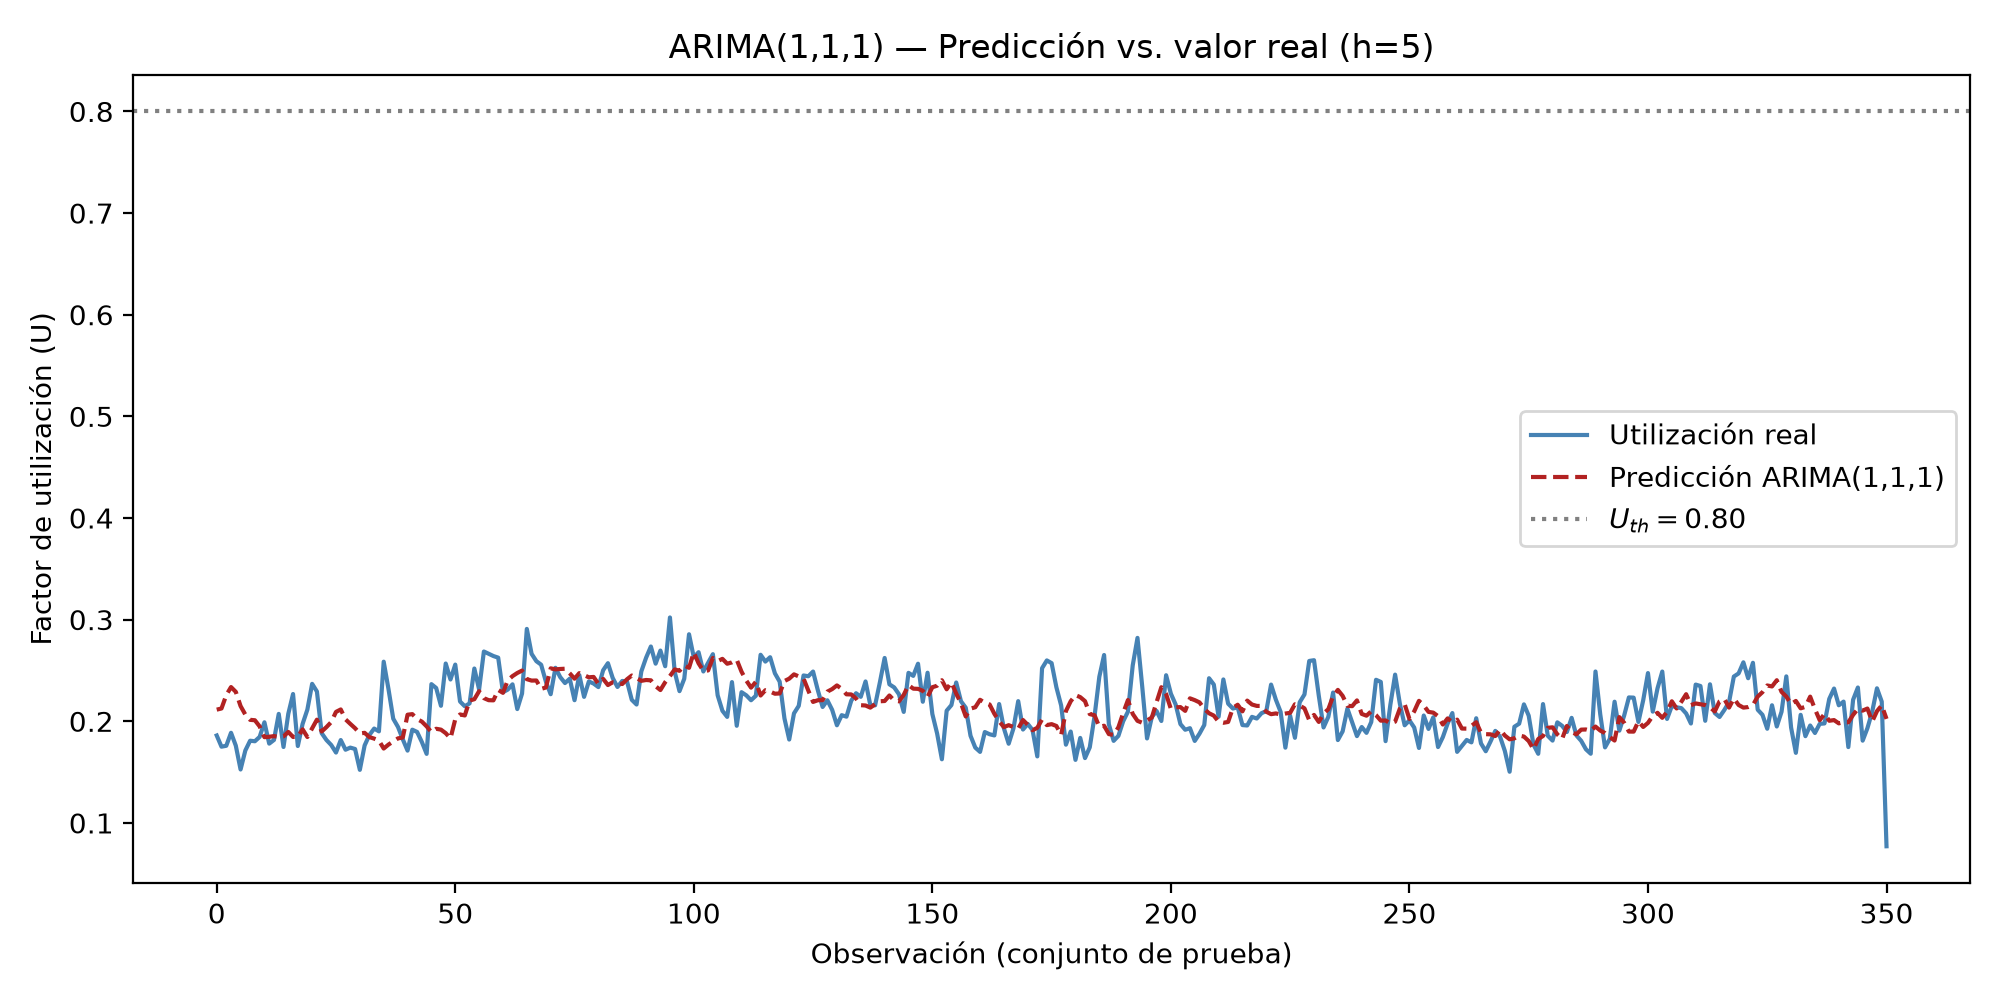
\includegraphics[width=0.85\textwidth]{arima_prediccion_vs_real.png}
    \caption{ARIMA(1,1,1): pronóstico progresivo ($h=5$) frente al valor real, partición de prueba del piloto MAWI.}
    \label{fig:arima_prediccion}
\end{figure}

En la Figura \ref{fig:arima_prediccion}, la predicción (línea roja discontinua) funciona como una versión suavizada de la utilización real (línea azul): la serie observada presenta oscilaciones de corto plazo con aspecto de ruido, mientras que el modelo traza únicamente la tendencia central. Este suavizado explica el error moderado y estable en regresión, pero tiene una contraparte: la inercia del modelo lo hace lento ante cambios súbitos, lo que se refleja en la clasificación.

\subsection*{Fase piloto: clasificación}

Con el umbral oficial $U_{th}=0.80$ la clasificación no es evaluable en MAWI, porque su utilización máxima es de 32.3\,\% (Sección \ref{sec:obtencion_exploracion}). Para ejercitar el código de evaluación se usó el umbral relativo de prueba $U_{test}=0.25$. La Tabla \ref{tab:resultados_arima_clasificacion} muestra el desempeño como clasificador de alertas tempranas sobre la partición de prueba.

\begin{table}[H]
    \centering
    \begin{tabular}{|l|r|}
        \hline
        \textbf{Métrica ($U_{test} \geq 0.25$)} & \textbf{Prueba} \\
        \hline
        Precisión & 64.2\,\% \\
        \textit{Recall} & 41.5\,\% \\
        \textit{F1-score} & 50.4\,\% \\
        \textbf{Tiempo de Anticipación Efectivo (TAE) promedio} & \textbf{1.2 minutos} \\
        \hline
    \end{tabular}
    \caption{Clasificación y alertamiento (TAE) de ARIMA(1,1,1), fase piloto.}
    \label{tab:resultados_arima_clasificacion}
\end{table}

La precisión de 64.2\,\% indica que cerca de dos de cada tres alertas corresponden a un evento real, mientras que el \textit{recall} de 41.5\,\% indica que el modelo deja pasar casi seis de cada diez eventos. El $TAE$ de 1.2 minutos queda muy por debajo del horizonte objetivo de 5 minutos: aun cuando acierta, el modelo alerta con poca antelación, coherente con el suavizado observado en regresión. Estas cifras validan el funcionamiento del \textit{pipeline}, pero no son comparables con las del \textit{dataset} primario, que usan otro umbral y otros datos.

\subsection*{\textit{Dataset} primario: regresión}

La Tabla \ref{tab:arima_primario_regresion} presenta el error de ARIMA(3,0,3) sobre las particiones reales, en escala original de utilización. No se reporta MAPE, porque la utilización real, cercana a cero, vuelve inestable su denominador (Sección \ref{sec:evaluacion}).

\begin{table}[H]
    \centering
    \begin{tabular}{|l|r|r|}
        \hline
        \textbf{Conjunto} & \textbf{RMSE} & \textbf{MAE} \\
        \hline
        Validación (real) & 0.046045 & 0.015110 \\
        Prueba (real) & 0.045872 & 0.015059 \\
        \hline
    \end{tabular}
    \caption{Métricas de regresión de ARIMA(3,0,3), \textit{dataset} primario (escala original de utilización).}
    \label{tab:arima_primario_regresion}
\end{table}

El error es prácticamente idéntico en validación y prueba (RMSE de 0.0460 y 0.0459), lo que indica que su origen es sistemático y no una pérdida de generalización entre particiones. Sin embargo, resulta aproximadamente un 63\,\% mayor que el del piloto (0.0459 frente a 0.0282), a pesar de que la utilización real del primario es mucho menor (máximo de 1.44\,\%, Tabla \ref{tab:estadisticas_real}) que la de MAWI (máximo de 32.3\,\%). Un RMSE de 0.0459 supera incluso la utilización máxima observada (0.0144), de modo que el error no puede deberse a la dificultad de seguir la señal, sino a un desajuste de nivel.

\begin{figure}[H]
    \centering
    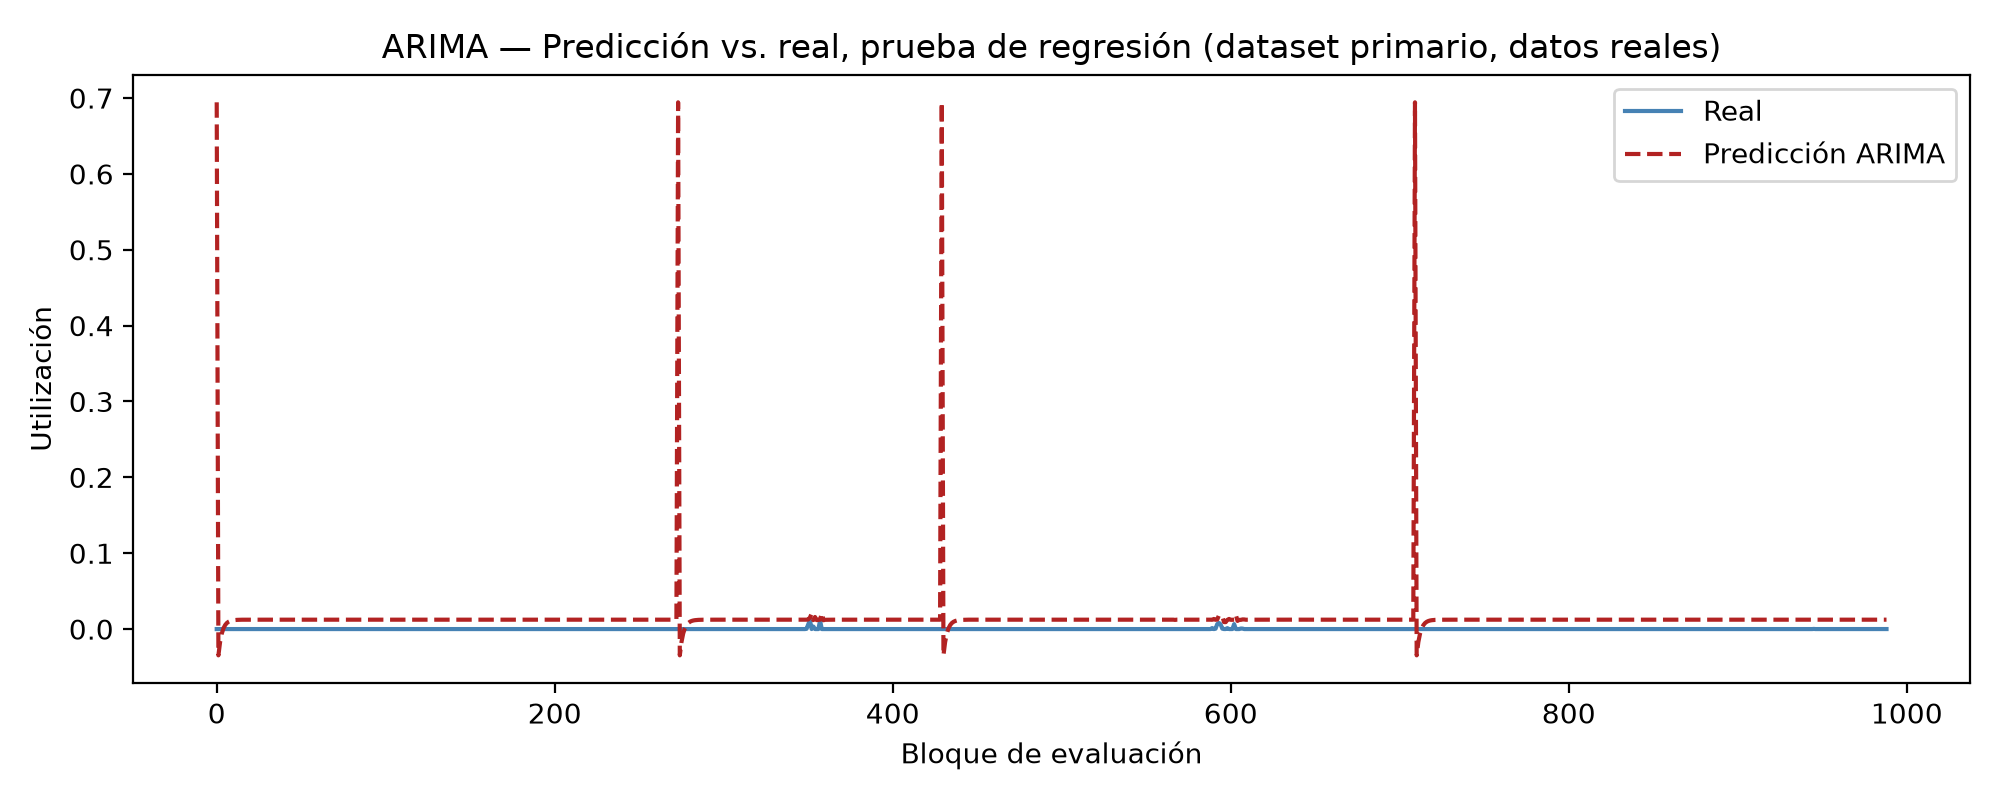
\includegraphics[width=0.85\textwidth]{arima_primario_regresion_test.png}
    \caption{ARIMA(3,0,3): predicción frente al valor real, prueba de regresión (\textit{dataset} primario, datos reales).}
    \label{fig:arima_primario_regresion}
\end{figure}

La Figura \ref{fig:arima_primario_regresion} permite identificar dos fenómenos. El primero es un sesgo sistemático de sobreestimación: la predicción de fondo (línea roja discontinua) se mantiene por encima de la señal real, que es plana y cercana a cero (línea azul). Esto es consistente con la media del proceso ajustado ($\mu=0.0324$), elevada por los eventos sintéticos de la sesión de ajuste, que rozan la saturación (hasta 0.98), mientras que el comportamiento típico del canal real es muy inferior.

El segundo fenómeno son oscilaciones transitorias, con picos agudos de hasta cerca de 0.7 y valles que perforan el eje negativo, espaciadas a intervalos regulares. Esta regularidad coincide con el inicio de cada bloque del pronóstico progresivo, donde el modelo reinicia su estado autorregresivo y de media móvil asimilando de golpe las observaciones previas. Con coeficientes autorregresivos de gran magnitud y suma cercana a 1, un pequeño desajuste inicial tarda en disiparse. Por eso las oscilaciones se interpretan como un artefacto del esquema de evaluación por bloques y no como un error de cálculo, y elevan el RMSE por encima de lo que reflejaría el comportamiento en régimen estable.

\subsection*{\textit{Dataset} primario: clasificación}

La Tabla \ref{tab:arima_primario_clasificacion} reporta la clasificación sobre las particiones sintéticas aisladas, con $U_{th}=0.80$.

\begin{table}[H]
    \centering
    \begin{tabular}{|l|r|r|}
        \hline
        \textbf{Métrica} & \textbf{Validación} & \textbf{Prueba} \\
        \hline
        Exactitud & 0.9741 & 0.9750 \\
        Precisión & 0.6667 & 1.0000 \\
        \textit{Recall} & 0.0357 & 0.0185 \\
        \textit{F1-score} & 0.0678 & 0.0364 \\
        AUC-ROC & 0.8905 & 0.8939 \\
        \hline
    \end{tabular}
    \caption{Métricas de clasificación de ARIMA(3,0,3), $U_{th}=0.80$, datos sintéticos aislados.}
    \label{tab:arima_primario_clasificacion}
\end{table}

La tabla contiene una aparente contradicción: una exactitud de 0.975 junto con un \textit{recall} de 0.0185. Se explica por el desbalance de clases, pues los casos de congestión son una fracción mínima (cerca del 2.6\,\%), de modo que un modelo que casi nunca alerta acierta en la inmensa mayoría de las observaciones y obtiene una exactitud alta. Por eso la exactitud no es informativa en este problema y las métricas relevantes son el \textit{recall} y el \textit{F1-score}, ambos muy bajos. La precisión de 1.0 en prueba se apoya en un único acierto, por lo que dice poco por sí sola. En contraste, el AUC-ROC es alto (0.89), lo que indica que la predicción continua sí ordena los instantes de congestión por encima de los normales, aunque no los lleve a cruzar el umbral de decisión.

La Figura \ref{fig:recap_arima_clasificacion_metricas} presenta estas métricas de forma comparativa entre validación y prueba.

\begin{figure}[H]
    \centering
    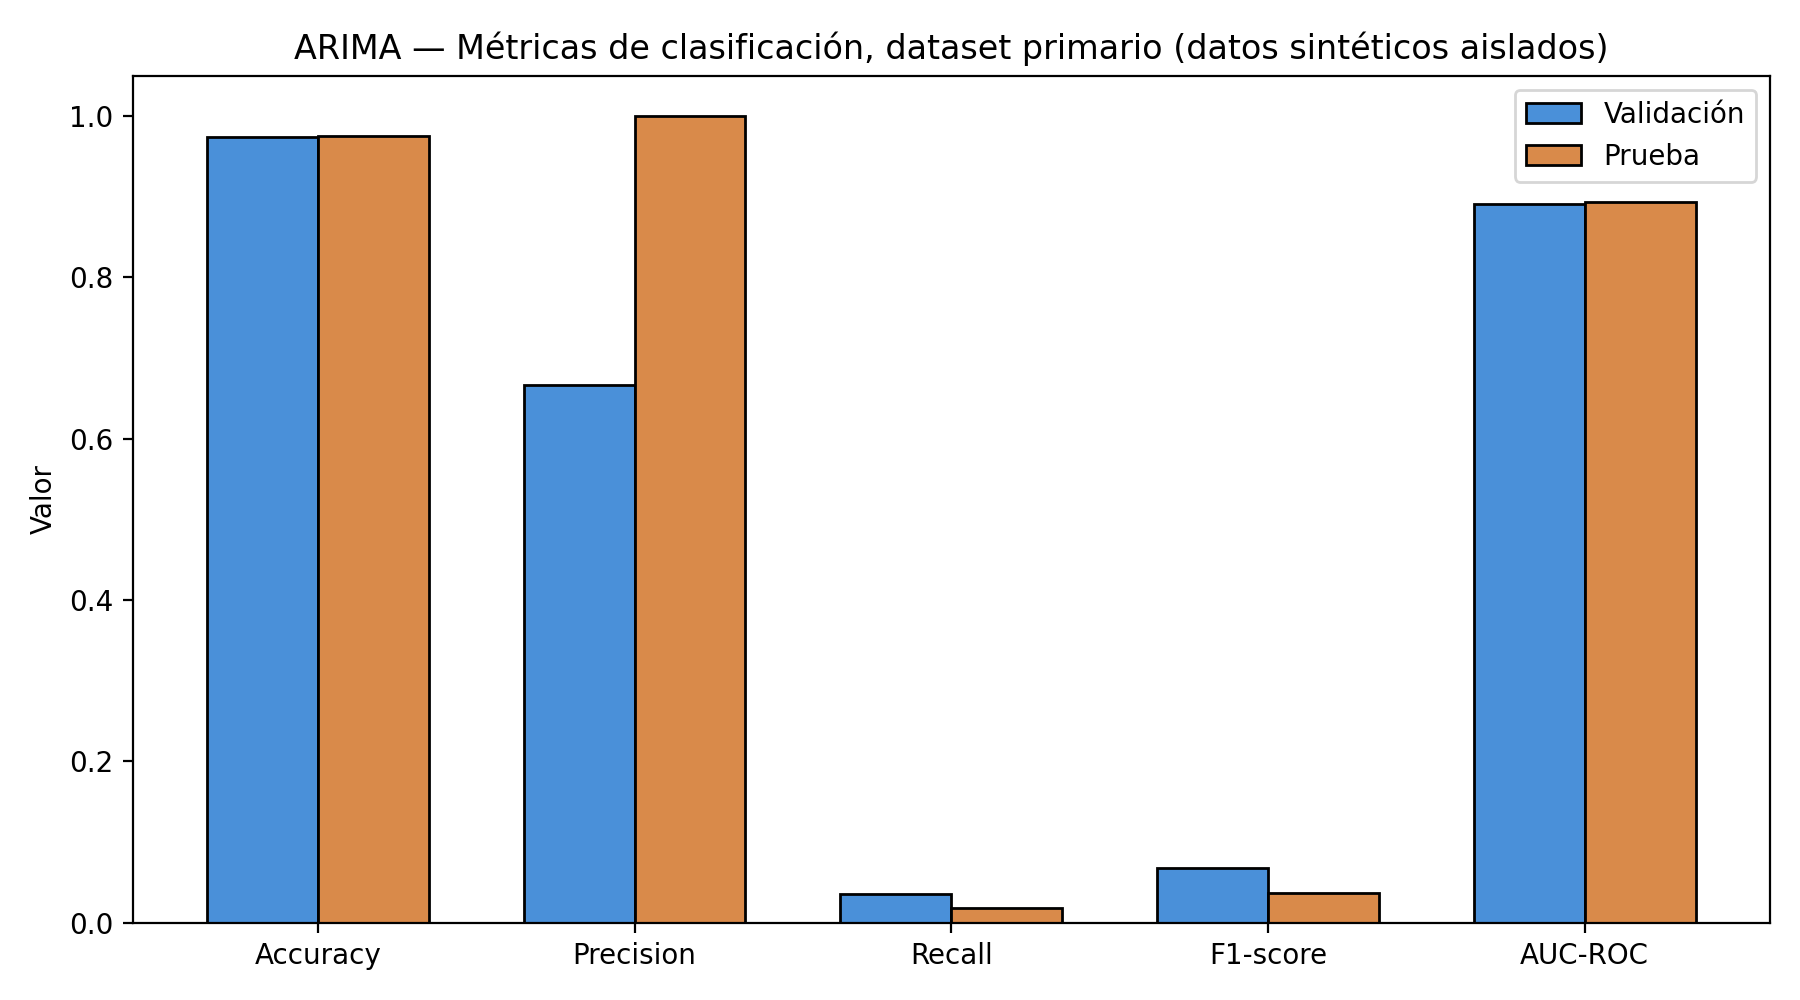
\includegraphics[width=0.8\textwidth]{arima_sintesis_clasificacion.png}
    \caption{Comparación de métricas de clasificación, validación frente a prueba, ARIMA sobre el \textit{dataset} primario.}
    \label{fig:recap_arima_clasificacion_metricas}
\end{figure}

La figura confirma que el patrón es el mismo en ambas particiones: exactitud y AUC-ROC elevados, y \textit{recall} y \textit{F1-score} cercanos a cero. La Ecuación \ref{eq:confusion_arima} presenta la matriz de confusión sobre la partición de prueba.

\begin{equation}
    \begin{pmatrix} \text{VN}=2070 & \text{FP}=0 \\ \text{FN}=53 & \text{VP}=1 \end{pmatrix}
    \label{eq:confusion_arima}
\end{equation}

Esta matriz describe el comportamiento del modelo frente al desbalance de clases:
\begin{itemize}
    \item \textbf{Verdaderos negativos (VN=2070):} el modelo reconoce correctamente los periodos de operación normal.
    \item \textbf{Falsos positivos (FP=0):} no emitió ninguna alerta injustificada, lo que explica la precisión de 100\,\%.
    \item \textbf{Falsos negativos (FN=53):} es el fallo crítico. De los 54 casos positivos, el modelo no alertó en 53, es decir, la red quedaría sin aviso ante casi todos los episodios de congestión.
    \item \textbf{Verdaderos positivos (VP=1):} solo se detectó un caso de congestión en toda la partición de prueba.
\end{itemize}

En términos operativos, un sistema que nunca da falsas alarmas pero que no avisa en el 98\,\% de las congestiones no resulta útil como mecanismo de alerta temprana.

\begin{figure}[H]
    \centering
    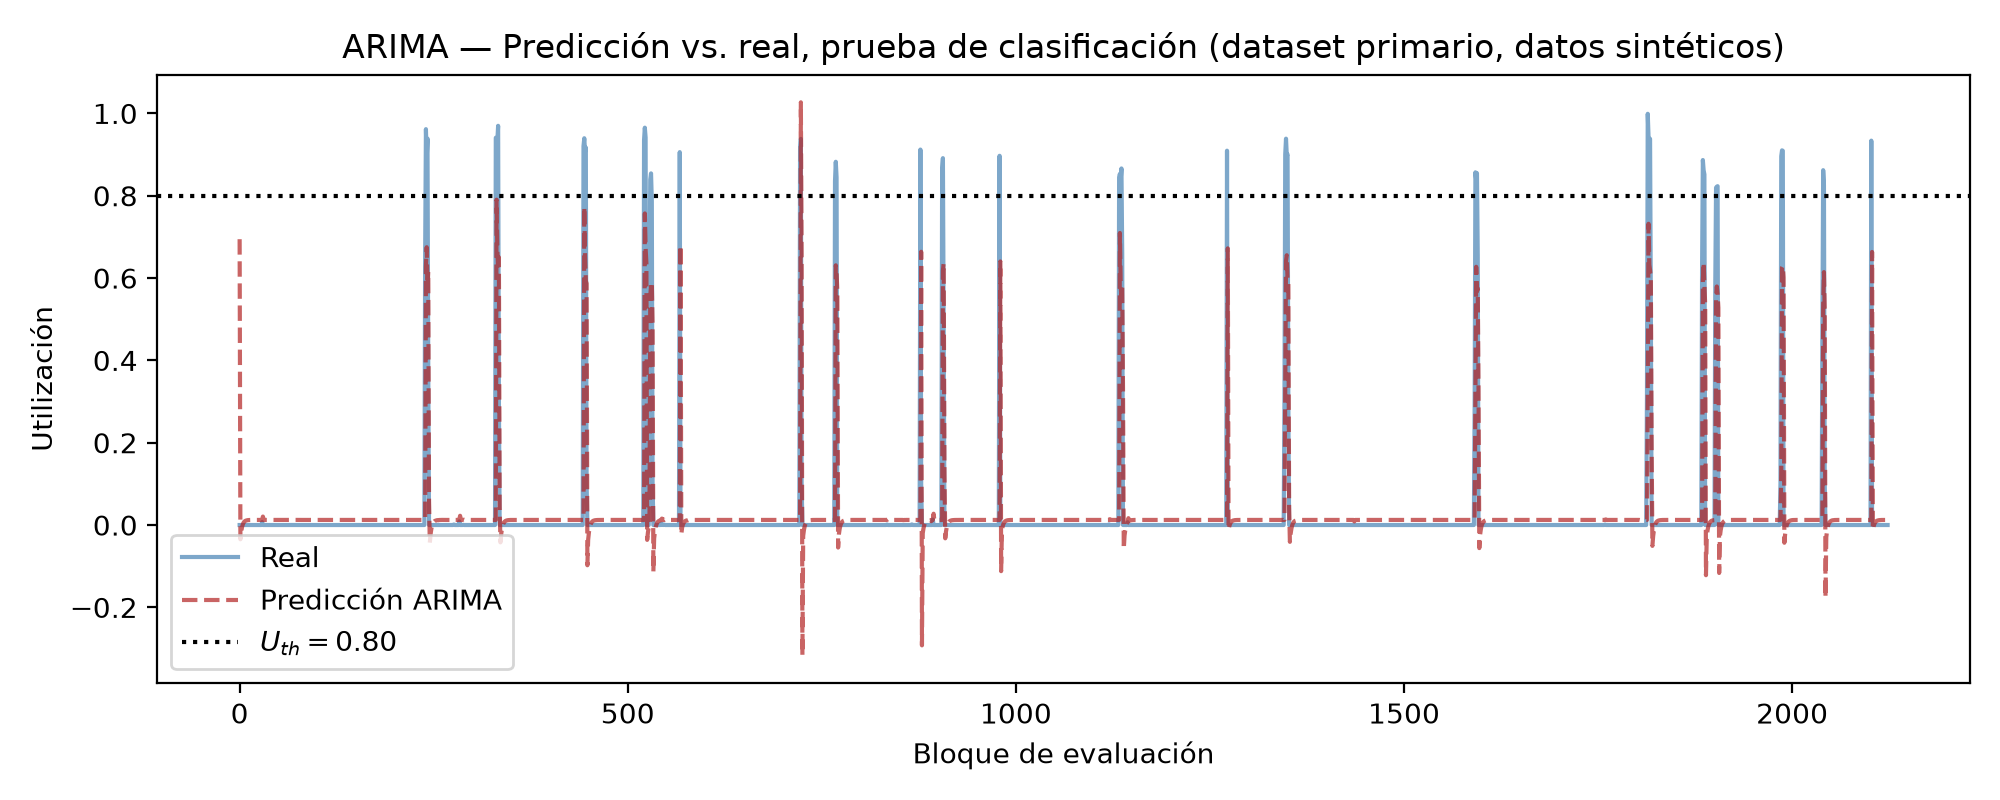
\includegraphics[width=0.85\textwidth]{arima_primario_clasificacion_test.png}
    \caption{ARIMA(3,0,3): predicción frente al valor real y umbral $U_{th}=0.80$, prueba de clasificación (\textit{dataset} primario, datos sintéticos aislados).}
    \label{fig:arima_primario_clasificacion}
\end{figure}

La Figura \ref{fig:arima_primario_clasificacion} muestra la causa de los falsos negativos. La predicción (línea roja discontinua) intenta seguir la trayectoria de los picos de utilización, pero con una amortiguación marcada: el componente de media móvil empuja el pronóstico hacia la tendencia central, y el modelo subestima sistemáticamente la magnitud de las ráfagas. Como consecuencia, las predicciones se quedan por debajo del umbral de 0.80 (línea punteada negra) y solo una lo cruza, lo que se traduce en un único verdadero positivo.

\subsection*{Validación de generalización (MAWI, granularidad oficial)}

Como prueba exploratoria, el ARIMA(3,0,3) entrenado con el \textit{dataset} primario se evaluó sobre MAWI reagregado a granularidad oficial de 1 minuto. La Tabla \ref{tab:recap_arima_generalizacion} presenta el resultado sobre las seis observaciones evaluables.

\begin{table}[H]
    \centering
    \begin{tabular}{|l|r|}
        \hline
        \textbf{Métrica} & \textbf{Valor} \\
        \hline
        RMSE & 0.323263 \\
        MAE & 0.236493 \\
        Observaciones evaluadas & 6 \\
        Rango real observado & [0.099, 0.213] \\
        \hline
    \end{tabular}
    \caption{Generalización de ARIMA(3,0,3) sobre MAWI (granularidad de 1 minuto).}
    \label{tab:recap_arima_generalizacion}
\end{table}

El RMSE de 0.323 equivale a casi el triple de la amplitud del rango real observado (0.114), de modo que el error medio supera con creces la variación total de la señal. Por el tamaño de la muestra (seis observaciones), el resultado es indicativo y no concluyente.

\begin{figure}[H]
    \centering
    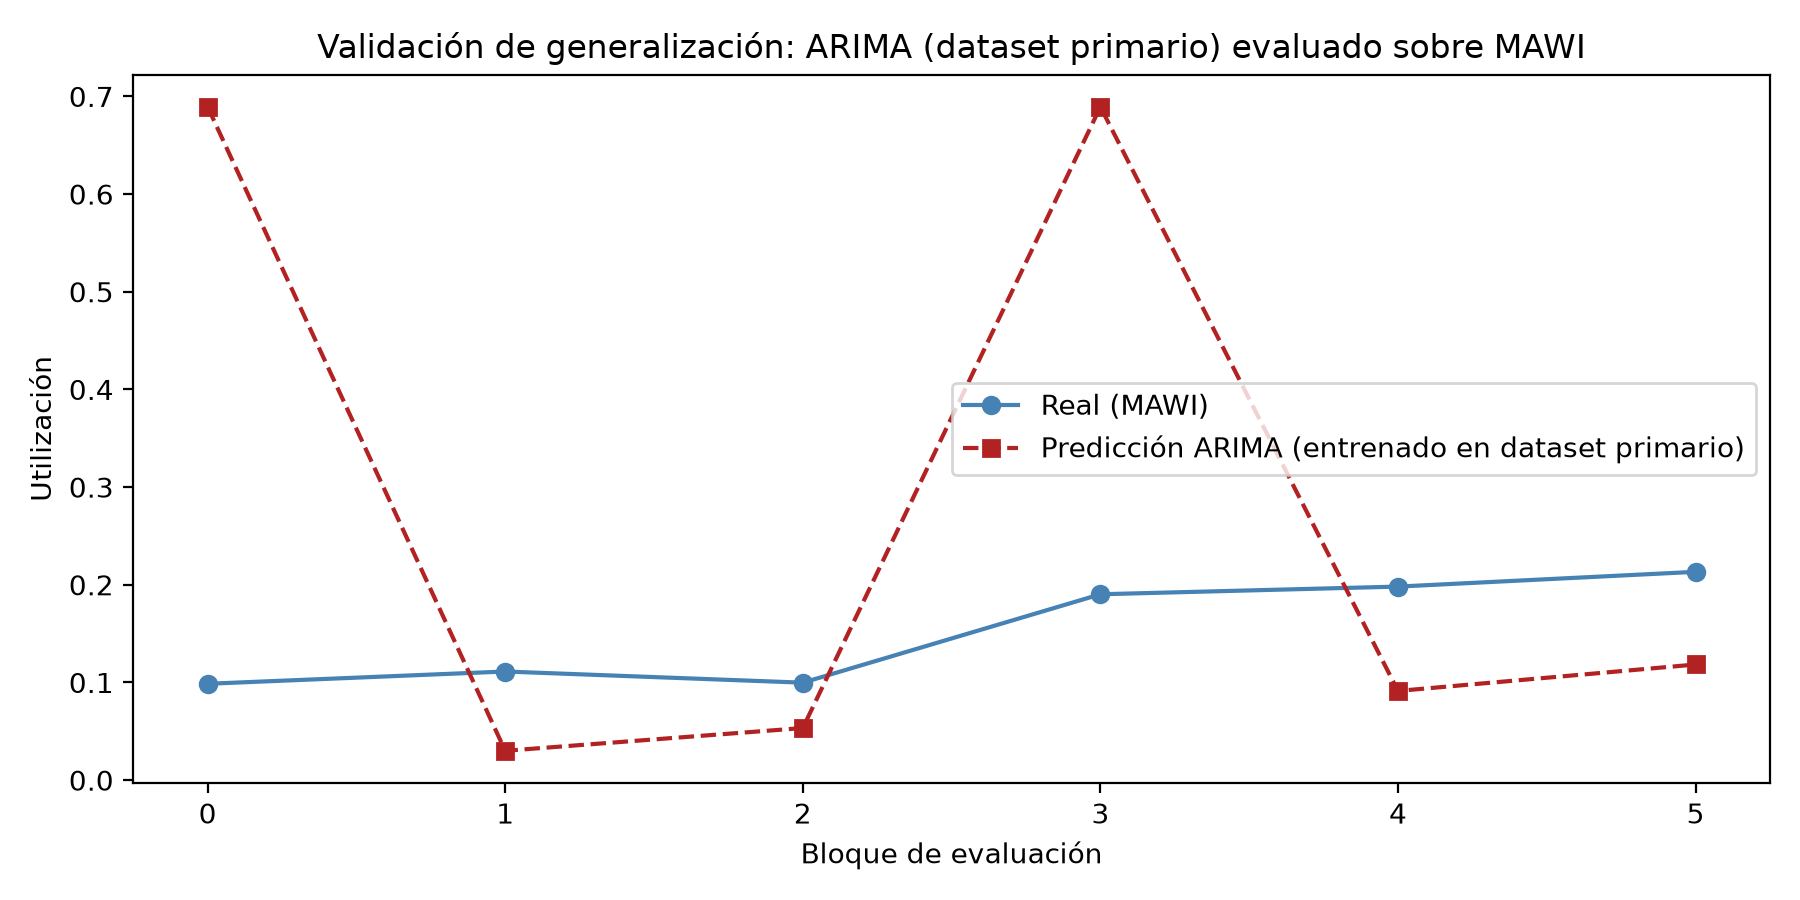
\includegraphics[width=0.85\textwidth]{arima_generalizacion_mawi.png}
    \caption{Generalización: ARIMA(3,0,3) entrenado con el \textit{dataset} primario y evaluado sobre MAWI.}
    \label{fig:recap_arima_generalizacion}
\end{figure}

La Figura \ref{fig:recap_arima_generalizacion} muestra que la trayectoria de predicción carece de correlación con la dinámica real. Mientras el tráfico real de MAWI se mantiene estable en torno a 0.15, las predicciones oscilan de forma violenta, con picos cercanos a 0.7 (bloques 0 y 3) seguidos de caídas hacia el cero. Los coeficientes autorregresivos y de media móvil se calibraron para un régimen con media cercana a cero y eventos de alta volatilidad (el primario); al recibir una serie con un nivel basal muy superior y otra varianza, el modelo sobrecorrige en cada bloque de evaluación.

\subsection*{Síntesis de los resultados de ARIMA}

La Figura \ref{fig:arima_sintesis_rmse} muestra la evolución del RMSE de regresión entre contextos de evaluación.

\begin{figure}[H]
    \centering
    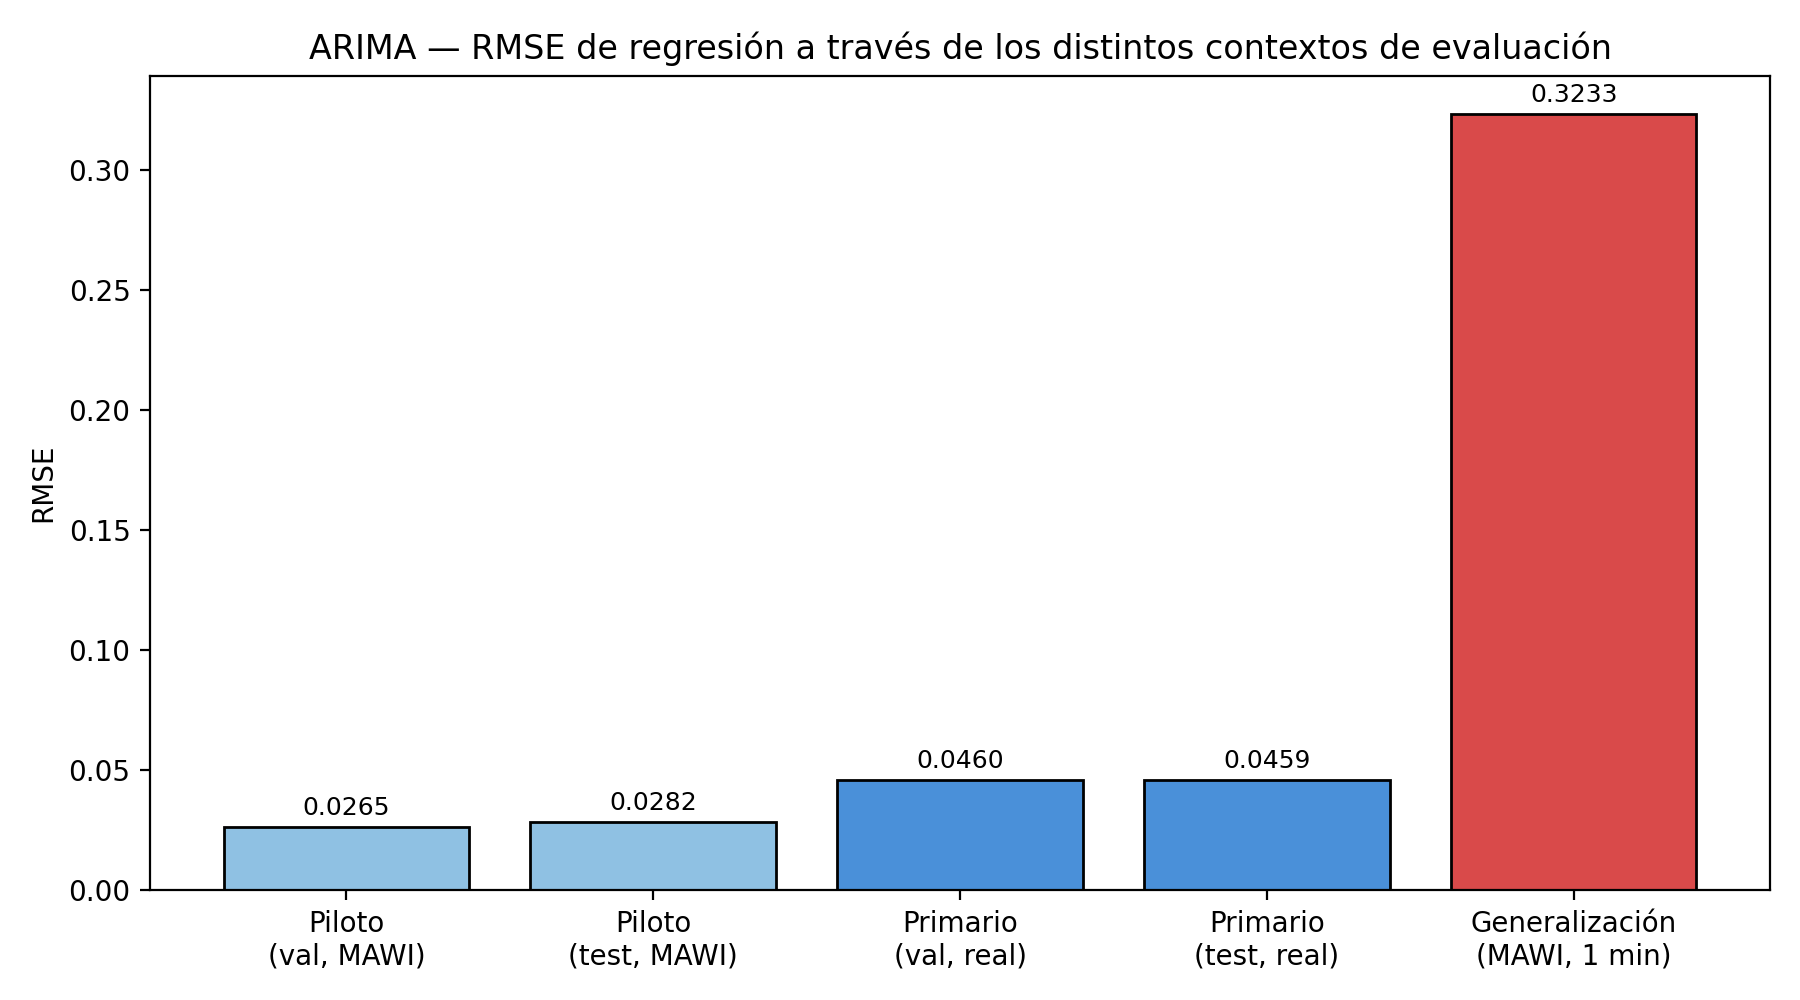
\includegraphics[width=0.85\textwidth]{arima_sintesis_rmse.png}
    \caption{RMSE de regresión de ARIMA en los contextos de evaluación.}
    \label{fig:arima_sintesis_rmse}
\end{figure}

La progresión de las barras muestra tres comportamientos:
\begin{itemize}
    \item \textbf{Piloto (0.0265 y 0.0282):} es el menor error del modelo. La serie de MAWI es relativamente homogénea y no contiene eventos de congestión, lo que permite que la ecuación autorregresiva promedie el ruido de fondo sin descompensaciones.
    \item \textbf{Primario (0.0460 y 0.0459):} el error basal aumenta cerca de un 63\,\%. Como la diferencia entre validación y prueba es prácticamente nula, no se explica por sobreajuste, sino por el sesgo de sobreestimación y el efecto del esquema por bloques descritos arriba.
    \item \textbf{Generalización (0.3233):} el error se multiplica por siete respecto al primario, lo que documenta que los coeficientes ajustados en una red no se transfieren a un régimen con otra distribución basal y otra varianza.
\end{itemize}

La Tabla \ref{tab:sintesis_completa_arima} reúne todas las métricas evaluadas y constituye la línea base contra la cual se contrastarán los modelos siguientes.

\begin{table}[H]
    \centering
    \small
    \begin{tabular}{|l|l|r|r|r|}
        \hline
        \textbf{Contexto} & \textbf{Naturaleza de los datos} & \textbf{RMSE} & \textbf{\textit{Recall}} & \textbf{AUC-ROC} \\
        \hline
        Piloto --- validación & 100\,\% real (MAWI) & 0.0265 & N/A & N/A \\
        Piloto --- prueba & 100\,\% real (MAWI) & 0.0282 & N/A & N/A \\
        Primario --- regresión (val.) & 100\,\% real & 0.0460 & --- & --- \\
        Primario --- regresión (prueba) & 100\,\% real & 0.0459 & --- & --- \\
        Primario --- clasificación (val.) & 100\,\% sintético & --- & 0.0357 & 0.8905 \\
        Primario --- clasificación (prueba) & 100\,\% sintético & --- & 0.0185 & 0.8939 \\
        Generalización --- MAWI (oficial) & 100\,\% real (MAWI) & 0.3233 & N/A & N/A \\
        \hline
    \end{tabular}
    \caption{Síntesis de los resultados de ARIMA. N/A: no aplicable con el umbral oficial (Sección \ref{sec:obtencion_exploracion}).}
    \label{tab:sintesis_completa_arima}
\end{table}

\subsection*{Discusión de los resultados de ARIMA}

\textbf{Regresión.} El RMSE sube de 0.0282 en el piloto a 0.0459 en el primario, pero esa comparación es limitada, porque son series distintas, con enlaces de 11 Gbps y 1 Gbps y dispersiones distintas. Lo revelador es la relación entre el error y la propia señal. En el piloto, el RMSE queda por debajo de la desviación estándar de la serie (0.051). En el primario, el RMSE (0.046) supera la utilización máxima observada (0.0144), mientras que una predicción constante igual a la media real tendría un error del orden de la desviación estándar de la serie (alrededor de $3.5 \times 10^{-4}$ en fracción). La causa más probable es el sesgo de sobreestimación de la Figura \ref{fig:arima_primario_regresion}: el modelo se ajustó sobre la sesión sintética, cuya media ($\mu=0.0324$) está elevada por los eventos inyectados y es muy superior a la real, de orden $10^{-5}$. Que el error sea casi idéntico en validación y prueba respalda que es sistemático y no un problema de generalización entre particiones.

\textbf{Oscilaciones por bloques.} Los picos y valles regulares de la Figura \ref{fig:arima_primario_regresion} están asociados al reinicio del estado autorregresivo al inicio de cada bloque del pronóstico progresivo. Con coeficientes AR de gran magnitud y suma cercana a 1, un pequeño desajuste inicial tarda en disiparse. Esto infla el RMSE sin reflejar la capacidad predictiva en régimen estable, de modo que es una limitación del esquema de evaluación por bloques que debe tenerse presente al comparar con los otros modelos.

\textbf{Clasificación.} El \textit{recall} de 1.85\,\% y el único verdadero positivo indican que, con el umbral de 0.80, el modelo prácticamente no alerta. Es consistente con la naturaleza de ARIMA: su componente de media móvil suaviza el pronóstico hacia la tendencia central, y rara vez la predicción puntual alcanza el umbral, aun durante un ascenso genuino. Esto concuerda con la limitación descrita en la Sección \ref{subsec:arima} sobre su naturaleza reactiva, a lo que se suma ahora un comportamiento excesivamente conservador frente a la congestión. En la fase piloto, con un umbral más bajo (0.25), el \textit{recall} fue mayor (41.5\,\%), lo que sugiere que parte del problema radica en la distancia entre el nivel predicho y el umbral exigido.

\textbf{Calibración del umbral.} El AUC-ROC alto (0.89) matiza la conclusión anterior: la predicción continua conserva información sobre la congestión, y el fallo parece estar en la decisión binaria sobre una predicción amortiguada, más que en la ausencia total de señal. Ajustar el umbral a partir de la validación no se exploró en este trabajo y es una línea de mejora para el diseño de alertas.

\textbf{Generalización.} El colapso sobre MAWI indica que los coeficientes de ARIMA están muy ligados al régimen donde se ajustaron. Una explicación probable es que los valores de MAWI (cerca de 0.15) caen fuera del rango del tráfico real del primario (máximo de 0.0144), y con coeficientes autorregresivos de signo alternante esa diferencia de nivel se amplifica. Por el tamaño de la muestra y el reinicio por bloques, esta explicación debe tomarse como hipótesis. Aun así, la evidencia desaconseja tratar a ARIMA como modelo transferible entre redes de escala distinta sin reajustarlo.

\textbf{Alcance.} En conjunto, ARIMA cumple como línea base de regresión sobre tráfico estable, pero su desempeño depende de que la serie de ajuste represente el régimen donde se evalúa, y no sirve como detector de congestión con el umbral oficial. Esta conclusión se contrasta con \textit{Random Forest} y LSTM en las Secciones 6.4 y 6.5.

\section{Resultados de \textit{Random Forest}}
\label{sec:resultados_rf}

Esta sección reporta los resultados del ensamble \textit{Random Forest}, configurado según la Sección \ref{sec:rf_desarrollo}: su desempeño en la fase piloto con MAWI, su evaluación de regresión y clasificación sobre el \textit{dataset} primario, el análisis de importancia de variables en ambos conjuntos y las razones por las que no pudo someterse a la validación de generalización frente a MAWI. Cada resultado se acompaña de su lectura inmediata. La comparación con los demás modelos se presenta en la Sección 6.4 y la discusión conjunta en la Sección 6.5.

\subsection*{Fase piloto: regresión}

Sobre el piloto, el modelo se entrenó con 1\,044 secuencias, usando los rezagos y la media móvil con granularidad de 1 segundo. La Tabla \ref{tab:resultados_rf_regresion} presenta las métricas sobre las particiones de validación y prueba, en escala normalizada.

\begin{table}[H]
    \centering
    \begin{tabular}{|l|r|r|r|}
        \hline
        \textbf{Conjunto} & \textbf{RMSE} & \textbf{MAE} & \textbf{MAPE} \\
        \hline
        Validación & 0.0962 & 0.0721 & 12.83\,\% \\
        Prueba & 0.1311 & 0.1004 & 16.26\,\% \\
        \hline
    \end{tabular}
    \caption{Métricas de regresión de \textit{Random Forest} (escala normalizada), \textit{dataset} piloto MAWI.}
    \label{tab:resultados_rf_regresion}
\end{table}

El error aumenta de validación a prueba: el RMSE crece un 36\,\% y el MAPE pasa de 12.83\,\% a 16.26\,\%. En ARIMA, en cambio, el MAPE se mantuvo prácticamente igual en ambas particiones (10.61\,\% y 10.80\,\%, Sección \ref{sec:resultados_arima}). Para comparar con la línea base estadística, que se mantuvo en escala original, el RMSE de prueba se reescala por el rango de la variable de entrenamiento ($0.323 - 0.017 = 0.306$). Se obtiene un RMSE equivalente de aproximadamente $0.1311 \times 0.306 \approx 0.040$, un 42\,\% superior al de ARIMA (0.0282).

\begin{figure}[H]
    \centering
    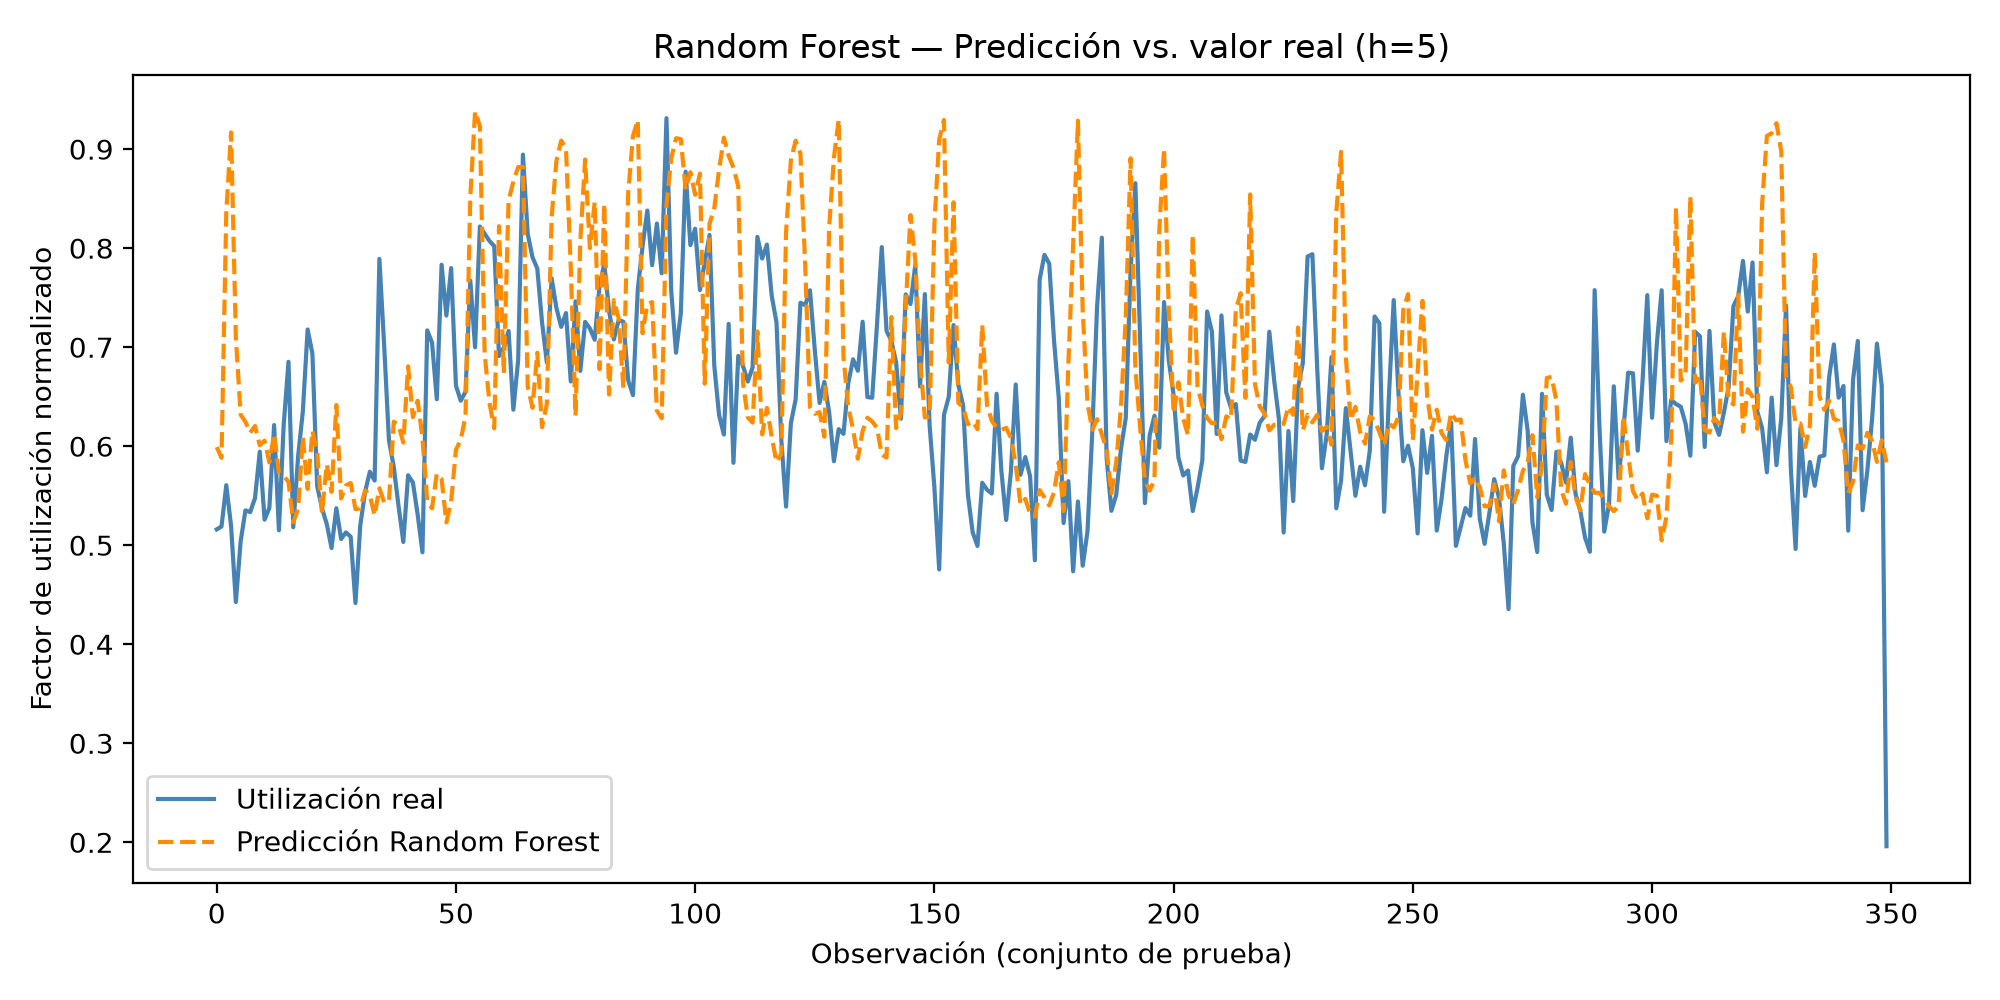
\includegraphics[width=0.85\textwidth]{rf_prediccion_vs_real.png}
    \caption{\textit{Random Forest}: predicción frente al valor real, partición de prueba del piloto MAWI (escala normalizada).}
    \label{fig:rf_prediccion}
\end{figure}

La Figura \ref{fig:rf_prediccion} muestra la causa de ese aumento. Cuando el tráfico real (línea azul) presenta caídas abruptas que llegan hasta cerca de 0.2 en el eje normalizado (por ejemplo, alrededor de la observación 350), la predicción del ensamble (línea naranja discontinua) tiene un piso visible y no desciende por debajo de aproximadamente 0.5. El modelo recorta, por tanto, los valles de la serie. Dado que cada hoja de un árbol predice el promedio de las muestras de entrenamiento que cayeron en ella, el ensamble tiende hacia valores centrales y responde poco a los extremos del comportamiento estocástico.

\subsection*{Fase piloto: clasificación}

Como en ARIMA, con el umbral oficial $U_{th}=0.80$ la clasificación no es evaluable en MAWI (Sección \ref{sec:obtencion_exploracion}), por lo que se usó el umbral relativo de prueba $U_{test} \geq 0.25$. La Tabla \ref{tab:resultados_rf_clasificacion} presenta el desempeño sobre la partición de prueba.

\begin{table}[H]
    \centering
    \begin{tabular}{|l|r|}
        \hline
        \textbf{Métrica ($U_{test} \geq 0.25$)} & \textbf{Prueba} \\
        \hline
        Precisión & 76.5\,\% \\
        \textit{Recall} & 68.3\,\% \\
        \textit{F1-score} & 72.1\,\% \\
        \textbf{Tiempo de Anticipación Efectivo (TAE) promedio} & \textbf{2.8 minutos} \\
        \hline
    \end{tabular}
    \caption{Clasificación y alertamiento (TAE) de \textit{Random Forest}, fase piloto.}
    \label{tab:resultados_rf_clasificacion}
\end{table}

Aproximadamente tres de cada cuatro alertas corresponden a un evento real (precisión de 76.5\,\%) y el modelo detecta cerca de dos tercios de los eventos (\textit{recall} de 68.3\,\%). Frente a ARIMA, el \textit{recall} sube 26.8 puntos porcentuales (de 41.5\,\% a 68.3\,\%) y el $TAE$ pasa de 1.2 a 2.8 minutos, más de la mitad del horizonte objetivo de 5 minutos. Como la regresión continua fue peor que la de ARIMA, el resultado muestra que el error medio de pronóstico y la capacidad de alertar son capacidades distintas. Estas cifras validan el \textit{pipeline}, pero no son comparables con las del \textit{dataset} primario, que usan otro umbral y otros datos.

\subsection*{Fase piloto: importancia de variables}

La Figura \ref{fig:rf_importancia} presenta la importancia relativa de las variables de entrada en el piloto, calculada como la disminución media de impureza que aporta cada una en los árboles.

\begin{figure}[H]
    \centering
    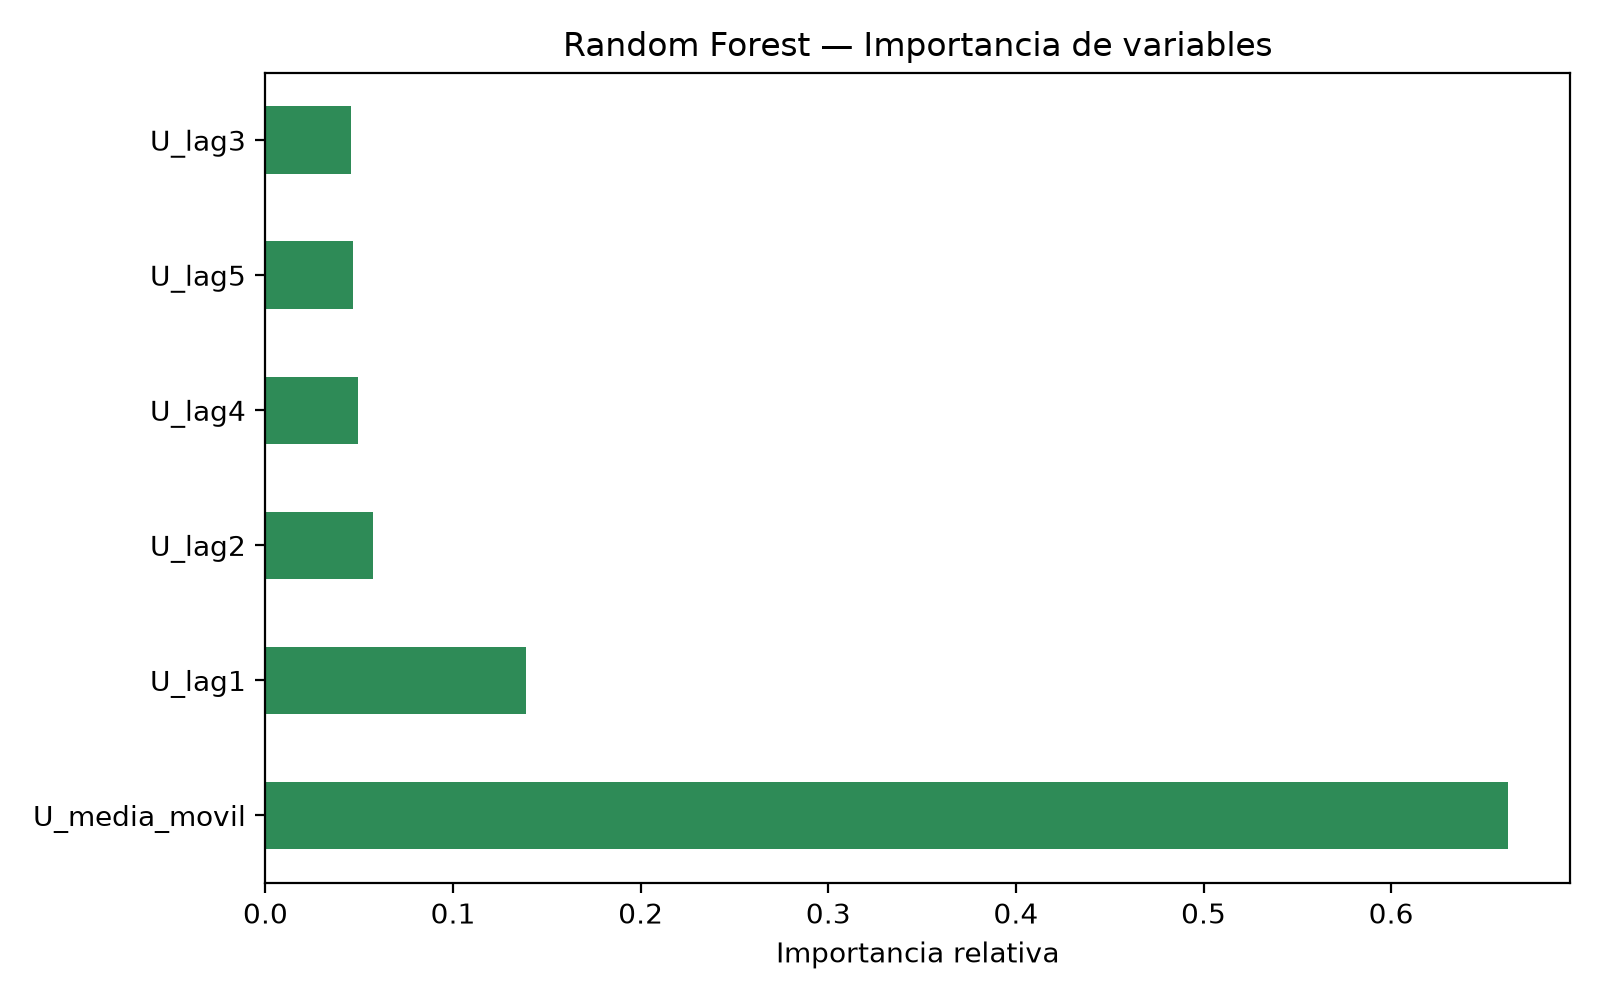
\includegraphics[width=0.75\textwidth]{rf_importancia_variables.png}
    \caption{Importancia relativa de variables en \textit{Random Forest}, \textit{dataset} piloto MAWI.}
    \label{fig:rf_importancia}
\end{figure}

La media móvil ($U_{\text{media\_movil}}$) concentra el 66.2\,\% de la importancia, muy por encima del rezago inmediato ($U_{\text{lag1}}$, 13.9\,\%). El 19.9\,\% restante se reparte entre los rezagos 2 a 5, cuya contribución individual es marginal. El modelo se apoya, entonces, sobre todo en el nivel promedio reciente y poco en el valor del instante anterior. Una explicación plausible es que, a una granularidad de 1 segundo, el valor inmediato está muy contaminado por ruido de alta frecuencia, y el promedio actúa como un filtro que revela la tendencia de fondo.

\subsection*{\textit{Dataset} primario: regresión}

La Tabla \ref{tab:rf_primario_regresion} presenta las métricas sobre las particiones reales, en escala normalizada. El modelo se reentrenó con la misma configuración sobre las 46\,872 observaciones de entrenamiento (reales y sintéticas).

\begin{table}[H]
    \centering
    \begin{tabular}{|l|r|r|}
        \hline
        \textbf{Conjunto} & \textbf{RMSE} & \textbf{MAE} \\
        \hline
        Validación (real) & 0.005084 & 0.004766 \\
        Prueba (real) & 0.049590 & 0.010301 \\
        \hline
    \end{tabular}
    \caption{Métricas de regresión de \textit{Random Forest}, \textit{dataset} primario (escala normalizada).}
    \label{tab:rf_primario_regresion}
\end{table}

El RMSE aumenta casi diez veces entre validación y prueba (de 0.0051 a 0.0496), mientras que en ARIMA se mantuvo constante sobre las mismas particiones (de 0.0460 a 0.0459). El MAE, sin embargo, solo se duplica (de 0.0048 a 0.0103). La relación entre ambas métricas es reveladora: en validación el RMSE es prácticamente igual al MAE (cociente de 1.07), lo que indica errores pequeños y uniformes, mientras que en prueba el cociente es de 4.8, lo que indica que el error se concentra en unas pocas desviaciones muy grandes. Esto coincide con la Figura \ref{fig:rf_primario_regresion_test}. Como el rango de entrenamiento está cerca de $[0,1]$ (los eventos sintéticos llegan a 0.979), la escala normalizada es aproximadamente equivalente a la original, de modo que el RMSE de prueba (0.0496) es del orden del de ARIMA (0.0459), y el MAE (0.0103) es menor que el de ARIMA (0.0151). En ambos casos, el RMSE supera la utilización real máxima observada (0.0144).

\begin{figure}[H]
    \centering
    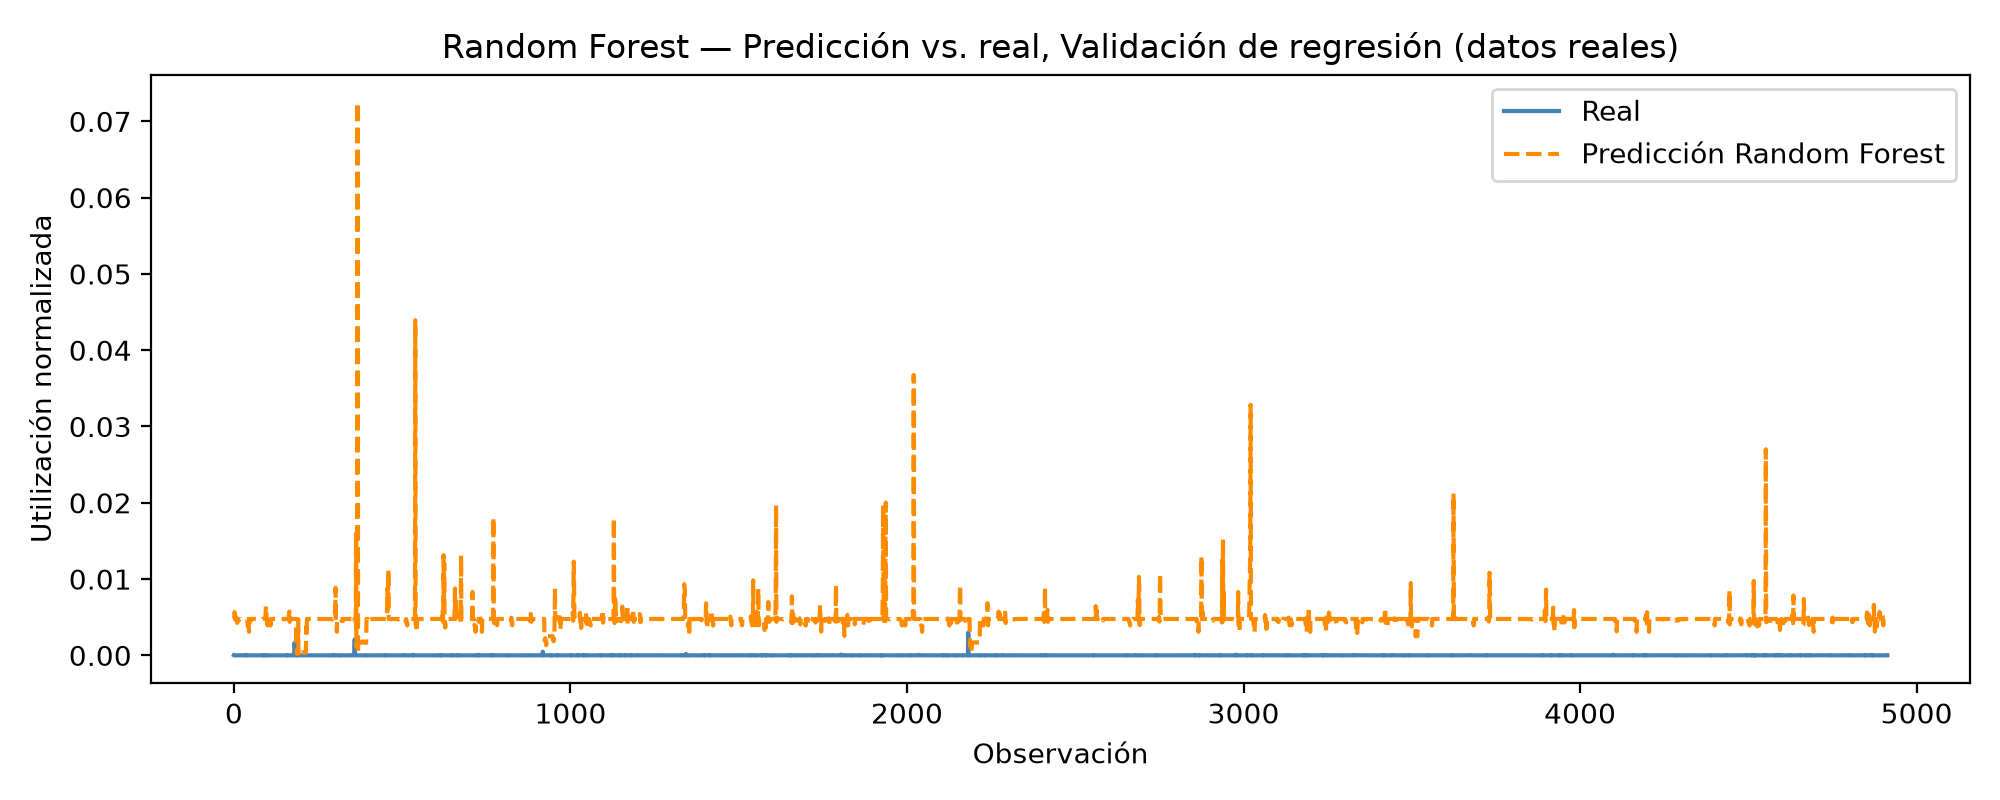
\includegraphics[width=0.85\textwidth]{rf_primario_regresion_val.png}
    \caption{\textit{Random Forest}: predicción frente al valor real, validación de regresión (\textit{dataset} primario, datos reales).}
    \label{fig:rf_primario_regresion_val}
\end{figure}

En validación (Figura \ref{fig:rf_primario_regresion_val}), la predicción (línea naranja discontinua) se mantiene cerca de la señal real, plana y cercana a cero. Presenta un sesgo leve de sobreestimación basal y picos transitorios que no superan 0.07 en la escala normalizada, por lo que no afectan de manera apreciable el RMSE.

\begin{figure}[H]
    \centering
    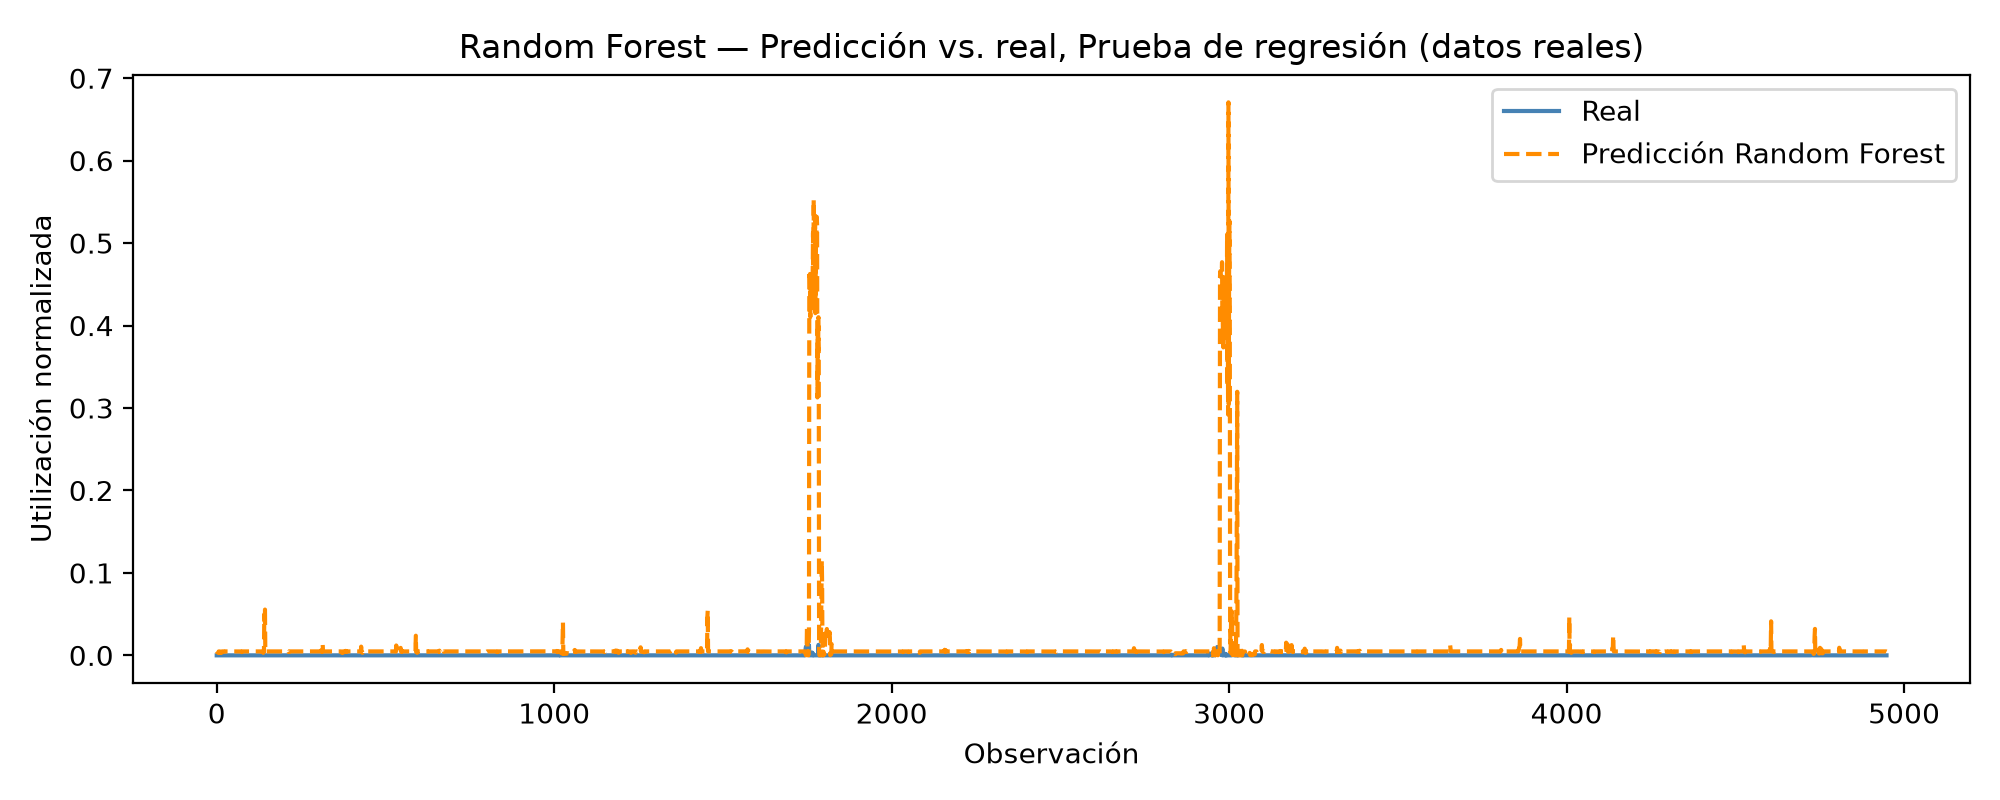
\includegraphics[width=0.85\textwidth]{rf_primario_regresion_test.png}
    \caption{\textit{Random Forest}: predicción frente al valor real, prueba de regresión (\textit{dataset} primario, datos reales).}
    \label{fig:rf_primario_regresion_test}
\end{figure}

En prueba (Figura \ref{fig:rf_primario_regresion_test}) el tráfico real sigue igual de plano, pero la predicción presenta dos picos de sobreestimación de gran magnitud, de aproximadamente 0.5 y casi 0.7 en la escala normalizada. Estos picos, que no corresponden a ningún evento real, explican prácticamente todo el aumento del RMSE.

\subsection*{\textit{Dataset} primario: síntesis del RMSE de regresión}

La Figura \ref{fig:rf_sintesis_rmse} muestra el RMSE de regresión del ensamble en los cuatro contextos de evaluación.

\begin{figure}[H]
    \centering
    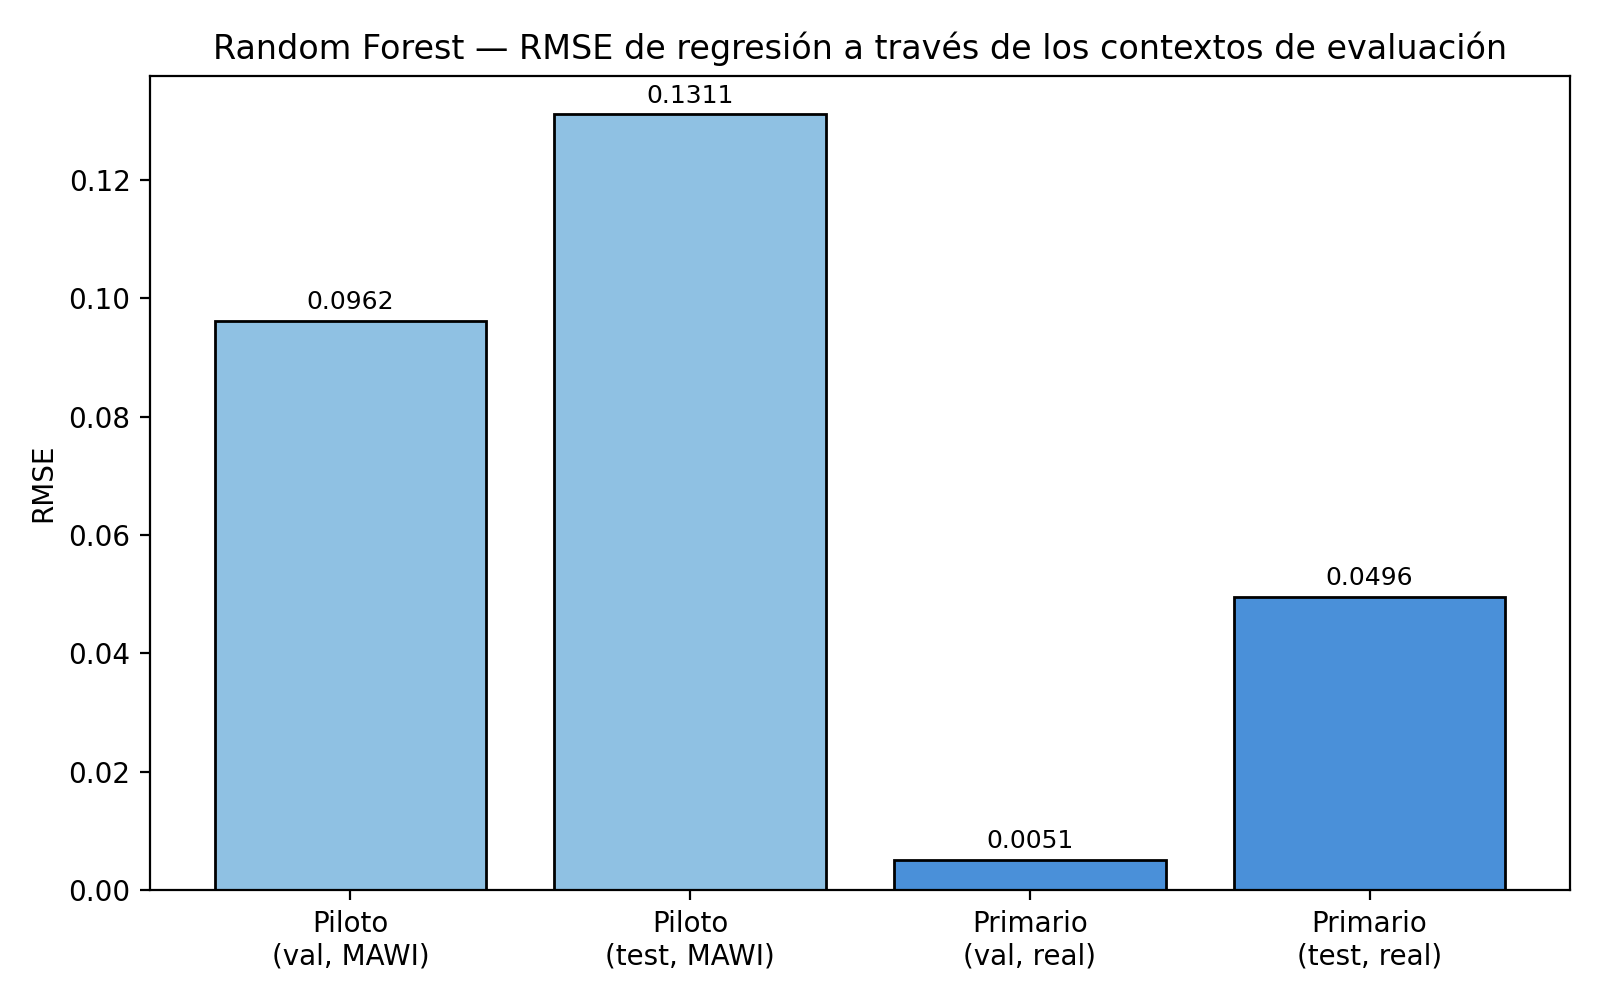
\includegraphics[width=0.85\textwidth]{rf_sintesis_rmse.png}
    \caption{RMSE de regresión de \textit{Random Forest} en los contextos de evaluación (escala normalizada).}
    \label{fig:rf_sintesis_rmse}
\end{figure}

Las barras muestran dos comportamientos:
\begin{itemize}
    \item \textbf{Piloto (barras celestes, 0.0962 y 0.1311):} el error es elevado y empeora en prueba, asociado al piso de la predicción frente a las caídas profundas del tráfico (Figura \ref{fig:rf_prediccion}).
    \item \textbf{Primario (barras azules, 0.0051 y 0.0496):} el error de validación es muy bajo, pero en prueba aumenta casi un orden de magnitud por los dos picos espurios de la Figura \ref{fig:rf_primario_regresion_test}.
\end{itemize}

Los valores del piloto y del primario corresponden a series distintas, con escalas de normalización distintas, por lo que no deben compararse directamente entre sí.

\subsection*{\textit{Dataset} primario: clasificación}

La Tabla \ref{tab:rf_primario_clasificacion} presenta las métricas de clasificación sobre las particiones sintéticas aisladas, con $U_{th}=0.80$ (en escala normalizada).

\begin{table}[H]
    \centering
    \begin{tabular}{|l|r|r|}
        \hline
        \textbf{Métrica} & \textbf{Validación} & \textbf{Prueba} \\
        \hline
        Exactitud & 0.9803 & 0.9813 \\
        Precisión & 0.9121 & 0.9318 \\
        \textit{Recall} & 0.2923 & 0.2982 \\
        \textit{F1-score} & 0.4427 & 0.4518 \\
        AUC-ROC & 0.8796 & 0.9187 \\
        \hline
    \end{tabular}
    \caption{Métricas de clasificación de \textit{Random Forest}, $U_{th}=0.80$, datos sintéticos aislados.}
    \label{tab:rf_primario_clasificacion}
\end{table}

El desempeño es estable entre ambas particiones. Como en ARIMA, la exactitud alta (0.98) tiene poco valor informativo por el desbalance de clases, pues los casos de congestión son cerca del 2.6\,\% de las observaciones. Las métricas relevantes son la precisión, alta (0.93 en prueba), y el \textit{recall}, modesto (0.298), que dan un \textit{F1-score} de 0.45. El \textit{recall} es 16 veces el de ARIMA (0.0185), aunque esa comparación debe tomarse con cautela porque las matrices de confusión de ambos modelos no se calcularon sobre el mismo número de observaciones. Además, el AUC-ROC de \textit{Random Forest} (0.88 a 0.92) es parecido al de ARIMA (0.89), lo que sugiere que la mejora de \textit{recall} proviene sobre todo de que las predicciones alcanzan el umbral con mayor frecuencia, y no de una capacidad muy distinta para ordenar los instantes de congestión por encima de los normales.

\begin{figure}[H]
    \centering
    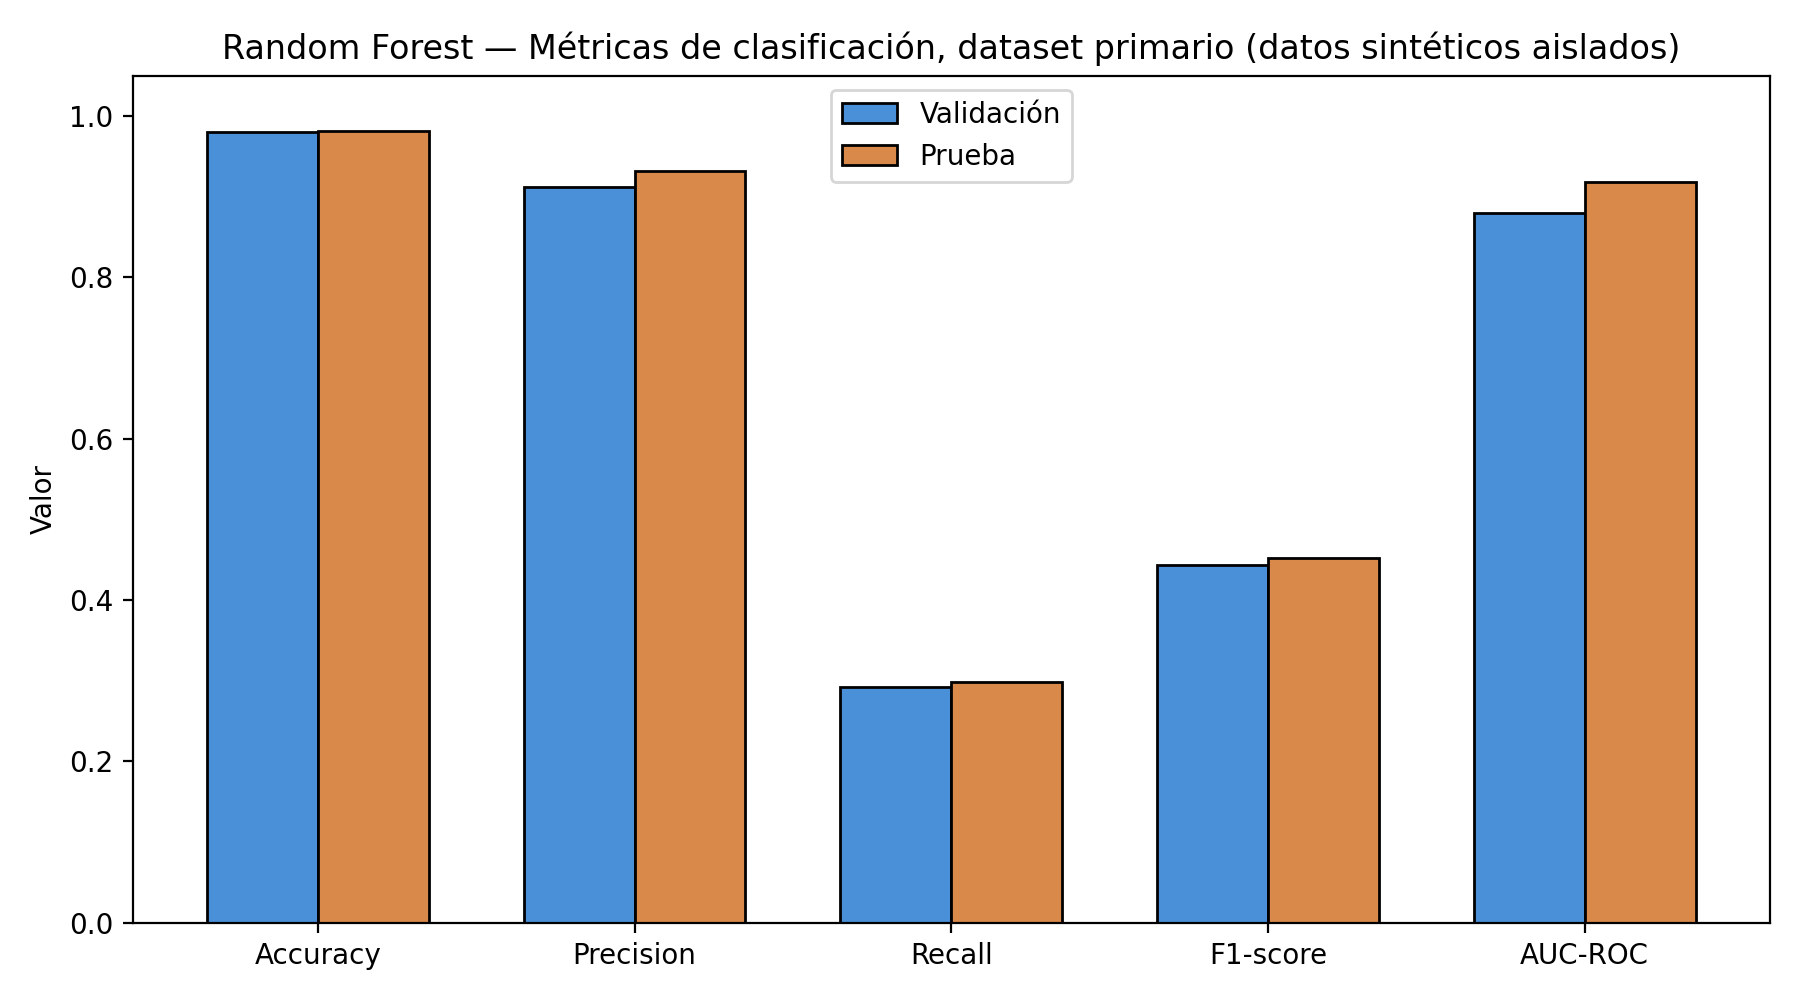
\includegraphics[width=0.8\textwidth]{rf_sintesis_clasificacion.png}
    \caption{Comparación de métricas de clasificación, validación frente a prueba, \textit{Random Forest} sobre el \textit{dataset} primario.}
    \label{fig:rf_sintesis_clasificacion}
\end{figure}

La Figura \ref{fig:rf_sintesis_clasificacion} confirma el patrón: exactitud, precisión y AUC-ROC altos, y \textit{recall} y \textit{F1-score} moderados en ambas particiones. La Ecuación \ref{eq:confusion_rf} presenta la matriz de confusión sobre la partición de prueba, cuya suma (10\,622 observaciones, 275 casos positivos) coincide con la Tabla \ref{tab:composicion_dataset_final}.

\begin{equation}
    \begin{pmatrix} \text{VN}=10\,341 & \text{FP}=6 \\ \text{FN}=193 & \text{VP}=82 \end{pmatrix}
    \label{eq:confusion_rf}
\end{equation}

Sus componentes se interpretan así:
\begin{itemize}
    \item \textbf{Verdaderos negativos (VN=10\,341):} el modelo reconoce correctamente los extensos periodos de operación normal.
    \item \textbf{Falsos positivos (FP=6):} solo seis falsas alarmas en todo el conjunto, equivalentes al 0.06\,\% de las observaciones normales. De ahí la precisión de 93.18\,\% (82 de 88 alertas fueron correctas).
    \item \textbf{Verdaderos positivos (VP=82):} de 275 instantes de congestión, se detectaron 82. Con ARIMA solo se detectó uno.
    \item \textbf{Falsos negativos (FN=193):} el 70\,\% de los instantes de congestión pasa sin alerta, lo que mantiene el \textit{recall} en 29.8\,\%.
\end{itemize}

En términos operativos, el modelo casi no genera ruido, pero omite siete de cada diez instantes de congestión. Con una precisión alta y un \textit{recall} moderado, el sistema sería confiable cuando alerta, pero insuficiente como única protección.

\begin{figure}[H]
    \centering
    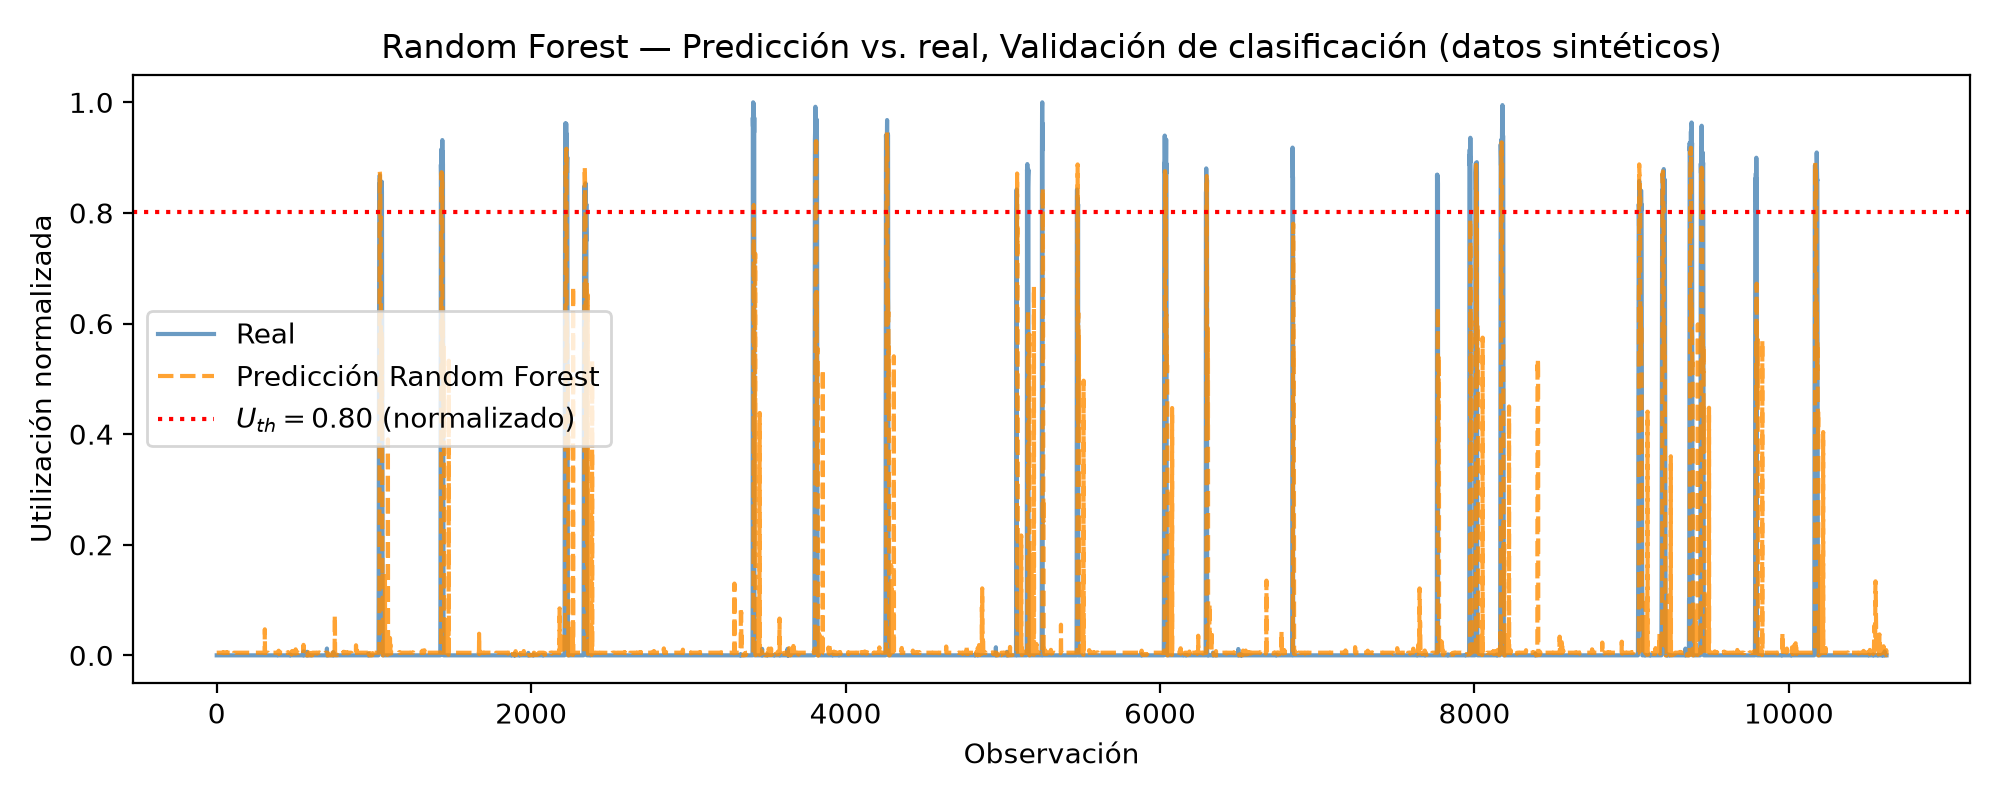
\includegraphics[width=0.85\textwidth]{rf_primario_clasificacion_val.png}
    \caption{\textit{Random Forest}: predicción frente al valor real y umbral $U_{th}=0.80$, validación de clasificación (\textit{dataset} primario, datos sintéticos aislados).}
    \label{fig:rf_primario_clasificacion_val}
\end{figure}

\begin{figure}[H]
    \centering
    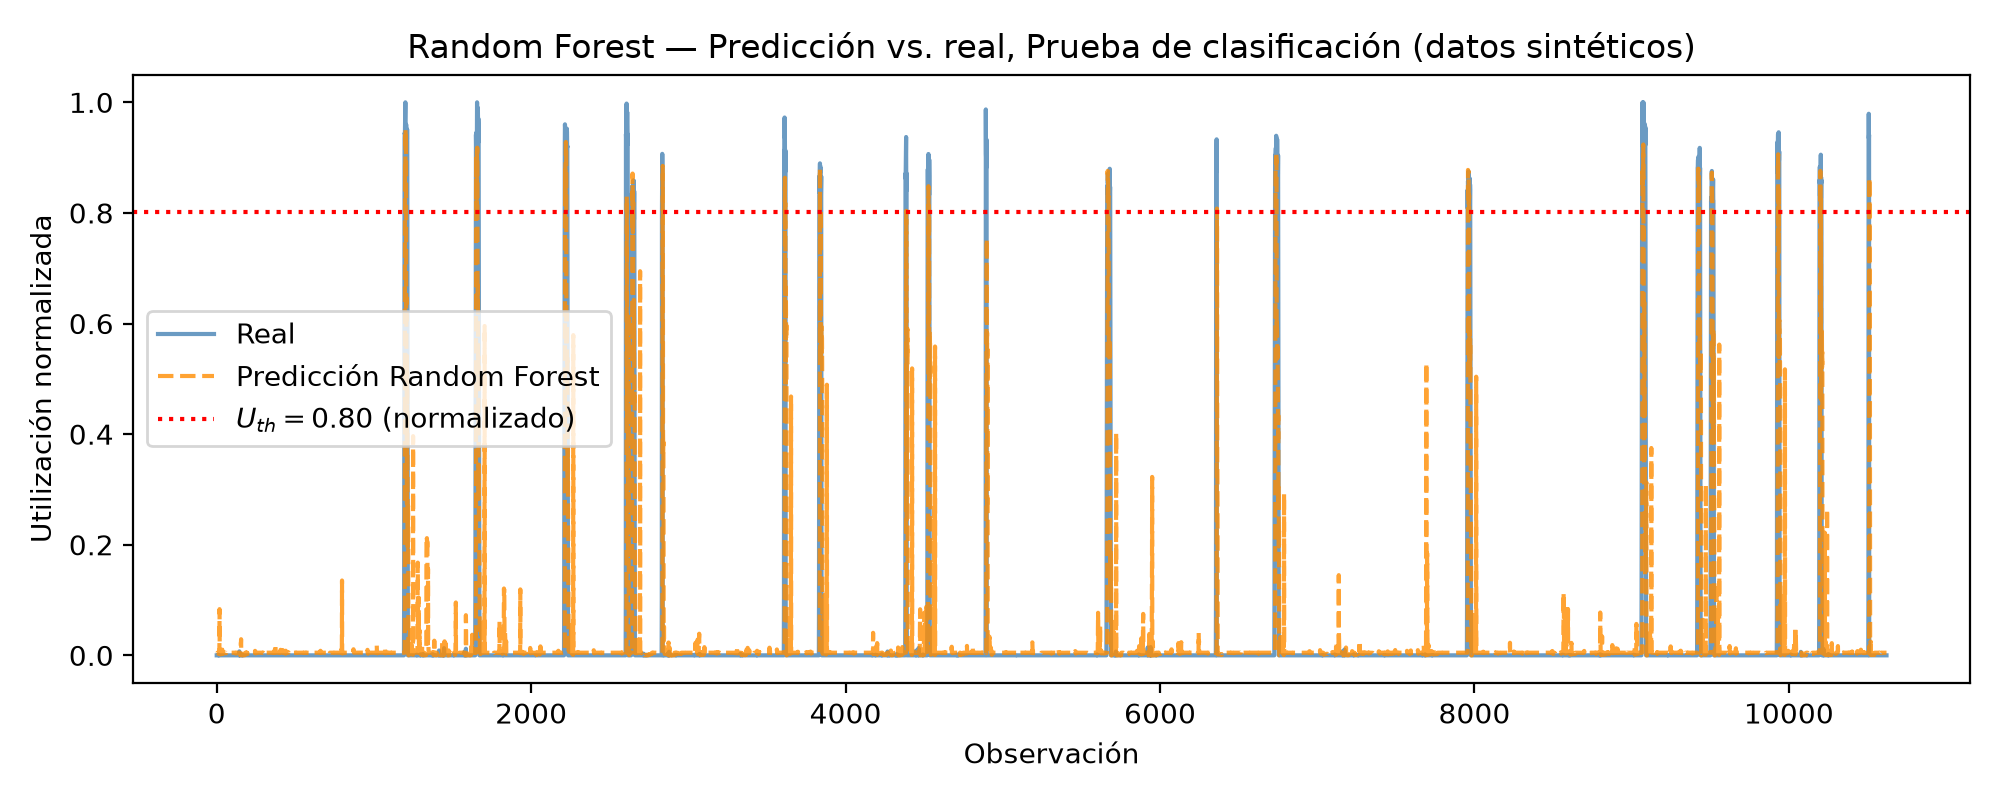
\includegraphics[width=0.85\textwidth]{rf_primario_clasificacion_test.png}
    \caption{\textit{Random Forest}: predicción frente al valor real y umbral $U_{th}=0.80$, prueba de clasificación (\textit{dataset} primario, datos sintéticos aislados).}
    \label{fig:rf_primario_clasificacion_test}
\end{figure}

Las Figuras \ref{fig:rf_primario_clasificacion_val} y \ref{fig:rf_primario_clasificacion_test} muestran el origen de los falsos negativos. A diferencia de ARIMA, cuya predicción se aplana, la del ensamble acompaña a los eventos: por cada pico del tráfico real aparece un pico de la predicción en el mismo momento. Sin embargo, la magnitud de muchos picos predichos es menor que la real, y varios se quedan justo por debajo del umbral de 0.80. El modelo identifica \textit{cuándo} ocurre el evento, pero no siempre estima su intensidad lo bastante alta para cruzar el umbral. El patrón es el mismo en validación y en prueba.

\subsection*{\textit{Dataset} primario: importancia de variables}

La Tabla \ref{tab:rf_primario_importancia} y la Figura \ref{fig:rf_primario_importancia} presentan la importancia relativa de cada variable en el \textit{dataset} primario.

\begin{table}[H]
    \centering
    \begin{tabular}{|l|r|}
        \hline
        \textbf{Variable} & \textbf{Importancia relativa} \\
        \hline
        $U_{\text{lag1}}$ & 0.6644 \\
        $U_{\text{media\_movil}}$ & 0.1249 \\
        $U_{\text{lag5}}$ & 0.1171 \\
        $U_{\text{lag2}}$ & 0.0320 \\
        $U_{\text{lag3}}$ & 0.0315 \\
        $U_{\text{lag4}}$ & 0.0301 \\
        \hline
    \end{tabular}
    \caption{Importancia relativa de variables, \textit{Random Forest}, \textit{dataset} primario.}
    \label{tab:rf_primario_importancia}
\end{table}

\begin{figure}[H]
    \centering
    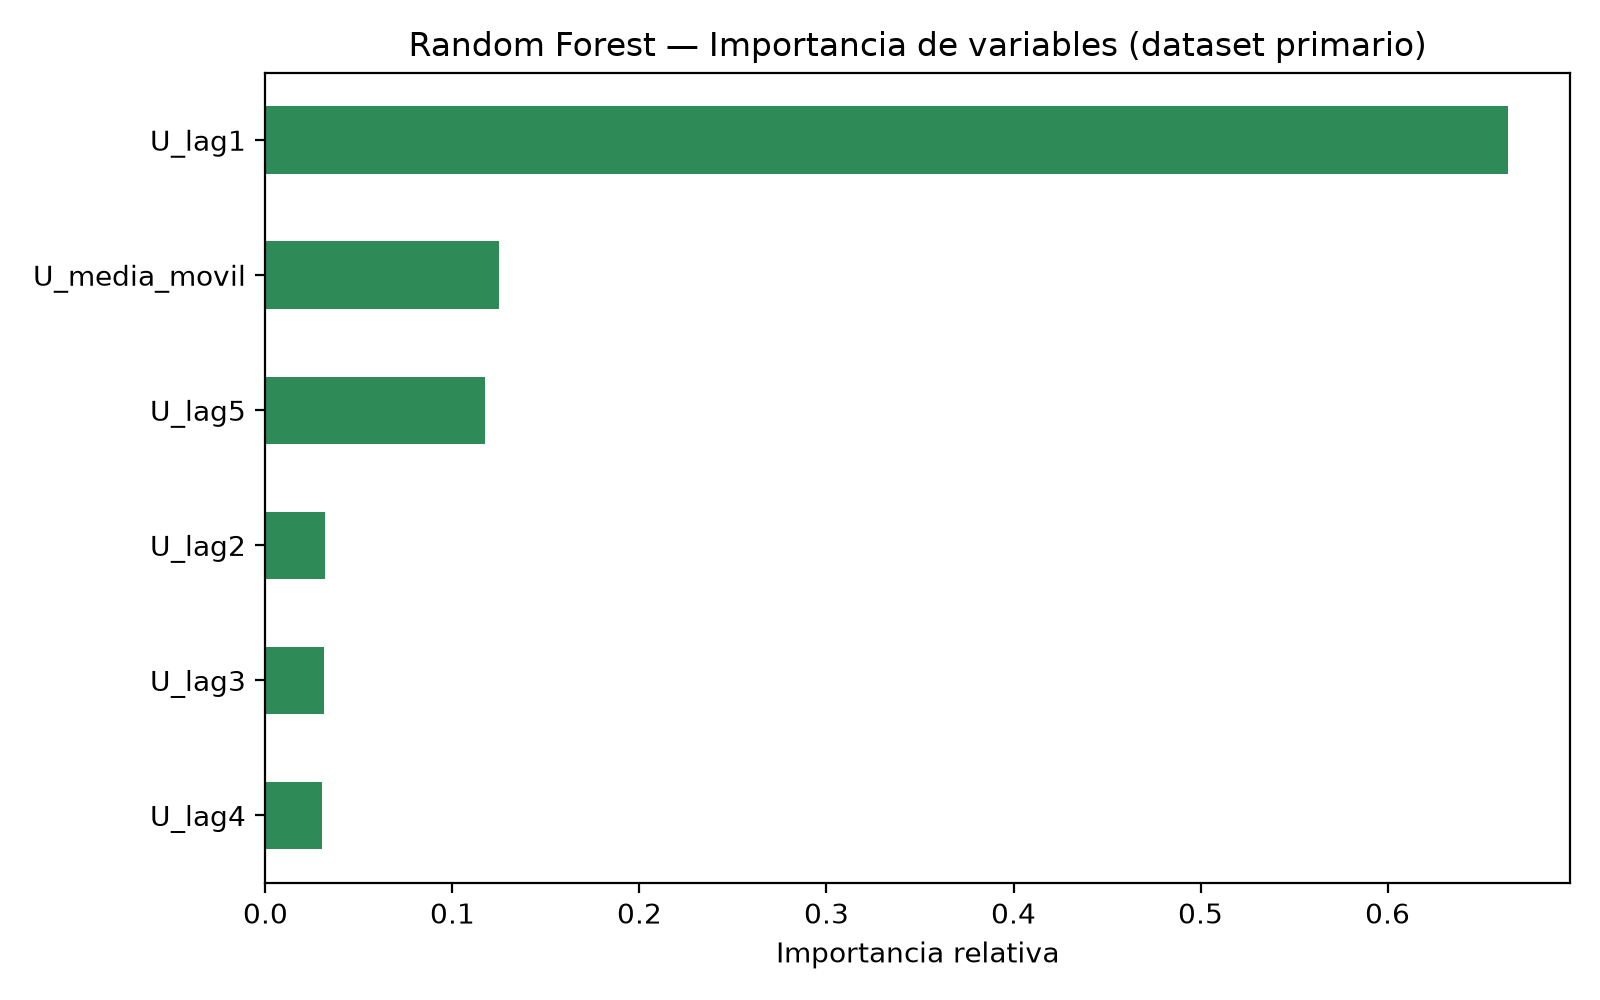
\includegraphics[width=0.75\textwidth]{rf_primario_importancia.png}
    \caption{Importancia relativa de variables en \textit{Random Forest}, \textit{dataset} primario.}
    \label{fig:rf_primario_importancia}
\end{figure}

El rezago inmediato concentra dos tercios de la importancia (66.4\,\%). Le siguen la media móvil (12.5\,\%) y el rezago más antiguo, $U_{\text{lag5}}$ (11.7\,\%), mientras que los rezagos 2 a 4 aportan alrededor del 3\,\% cada uno. Que el rezago 5 pese más que los intermedios sugiere que el modelo usa el contraste entre el valor más reciente y el más antiguo de la ventana, es decir, una señal de tendencia, aunque con estos datos no puede confirmarse.

\begin{figure}[H]
    \centering
    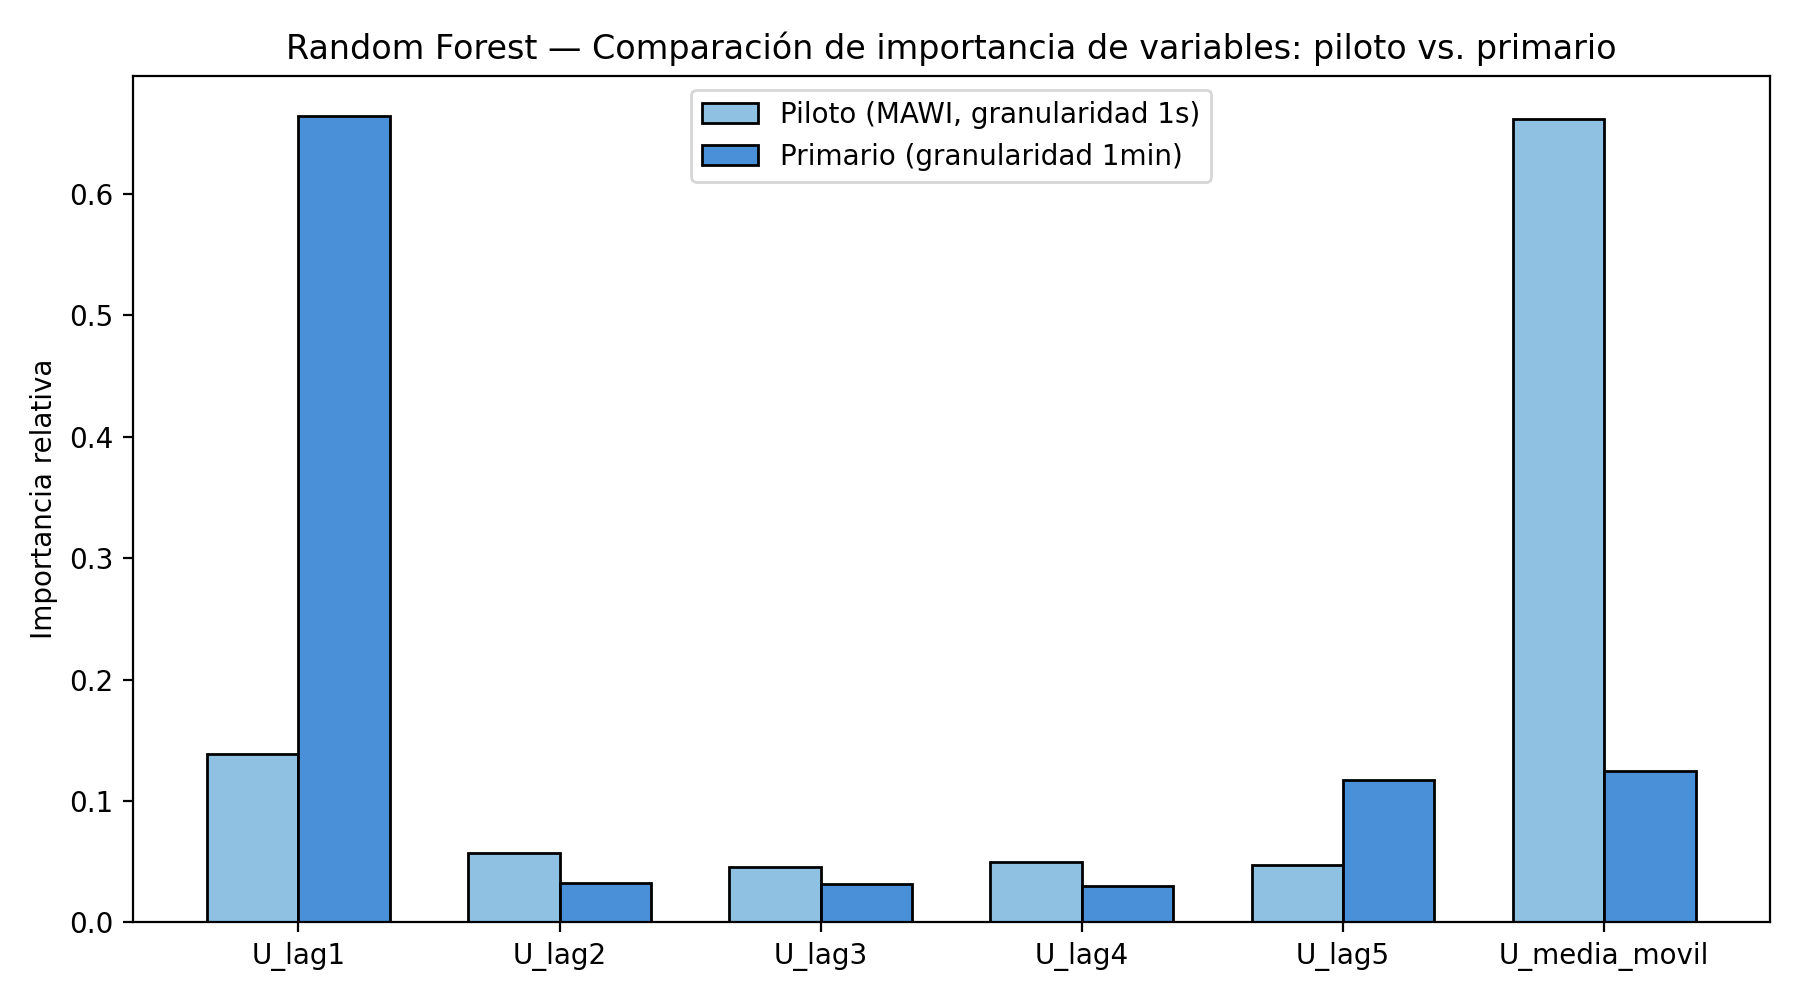
\includegraphics[width=\textwidth]{rf_comparativa_importancia.png}
    \caption{Importancia relativa de variables en \textit{Random Forest}: piloto frente al \textit{dataset} primario.}
    \label{fig:rf_comparativa_importancia}
\end{figure}

La Figura \ref{fig:rf_comparativa_importancia} contrasta ambos conjuntos y muestra una inversión casi simétrica: la media móvil pasa de 66.2\,\% a 12.5\,\% y el rezago inmediato, de 13.9\,\% a 66.4\,\%. La Tabla \ref{tab:comparativa_rf_piloto_primario} resume la comparación de la fase piloto con el \textit{dataset} primario.

\begin{table}[H]
    \centering
    \begin{tabular}{|l|r|r|}
        \hline
        \textbf{Métrica (prueba)} & \textbf{Piloto (MAWI)} & \textbf{Primario} \\
        \hline
        RMSE (regresión, normalizado) & 0.1311 & 0.0496 \\
        \textit{Recall} (clasificación) & 68.3\,\% ($U_{test}=0.25$) & 29.8\,\% ($U_{th}=0.80$) \\
        \textit{F1-score} (clasificación) & 72.1\,\% ($U_{test}=0.25$) & 45.2\,\% ($U_{th}=0.80$) \\
        Variable más importante & $U_{\text{media\_movil}}$ (66.2\,\%) & $U_{\text{lag1}}$ (66.4\,\%) \\
        \hline
    \end{tabular}
    \caption{Comparación de \textit{Random Forest} entre la fase piloto y el \textit{dataset} primario. Las métricas de clasificación usan umbrales distintos y no son directamente comparables.}
    \label{tab:comparativa_rf_piloto_primario}
\end{table}

\subsection*{Validación de generalización no realizada}

A diferencia de ARIMA (Sección \ref{sec:resultados_arima}), \textit{Random Forest} no pudo evaluarse sobre MAWI reagregado a la granularidad oficial de 1 minuto. La variable $U_{\text{media\_movil}}$ se calcula como una media móvil de 30 minutos (Sección \ref{sec:preprocesamiento_desarrollo}), y no puede construirse dentro de una traza de MAWI, que dura solo 15 minutos continuos (Sección \ref{sec:obtencion_exploracion}). Sin ese componente no se puede formar el vector de entrada que el ensamble espera. Rellenar con ceros o acortar la ventana alteraría la configuración validada y haría injusta cualquier comparación con ARIMA, por lo que esta validación se reporta como no realizada.

\subsection*{Síntesis de los resultados de \textit{Random Forest}}

La Tabla \ref{tab:sintesis_completa_rf} reúne las métricas de todos los contextos de evaluación.

\begin{table}[H]
    \centering
    \small
    \begin{tabular}{|l|l|r|r|r|}
        \hline
        \textbf{Contexto} & \textbf{Naturaleza de los datos} & \textbf{RMSE} & \textbf{\textit{Recall}} & \textbf{AUC-ROC} \\
        \hline
        Piloto --- validación & 100\,\% real (MAWI) & 0.0962 & N/A & N/A \\
        Piloto --- prueba & 100\,\% real (MAWI) & 0.1311 & N/A & N/A \\
        Primario --- regresión (val.) & 100\,\% real & 0.0051 & --- & --- \\
        Primario --- regresión (prueba) & 100\,\% real & 0.0496 & --- & --- \\
        Primario --- clasificación (val.) & 100\,\% sintético & --- & 0.2923 & 0.8796 \\
        Primario --- clasificación (prueba) & 100\,\% sintético & --- & 0.2982 & 0.9187 \\
        Generalización --- MAWI (oficial) & \multicolumn{4}{c|}{No evaluable (incompatibilidad estructural)} \\
        \hline
    \end{tabular}
    \caption{Síntesis de los resultados de \textit{Random Forest}. N/A: no aplicable con el umbral oficial (Sección \ref{sec:obtencion_exploracion}). Los RMSE están en escala normalizada.}
    \label{tab:sintesis_completa_rf}
\end{table}

\subsection*{Discusión de los resultados de \textit{Random Forest}}

\textbf{Regresión en el piloto.} El piso de la predicción frente a las caídas profundas (Figura \ref{fig:rf_prediccion}) es coherente con el promediado de las hojas: el árbol responde con el valor medio de las muestras de entrenamiento similares y suaviza los extremos. Esta limitación suele describirse como incapacidad de extrapolar, aunque en sentido estricto la extrapolación implica valores fuera del rango de entrenamiento, y una caída a 0.2 en escala normalizada está dentro del rango $[0,1]$. Una explicación alternativa es que esas caídas fueran poco frecuentes en la partición de entrenamiento y, por tanto, quedaran poco representadas en las hojas. Con estos datos no es posible distinguir entre ambas.

\textbf{Regresión en el primario.} El deterioro entre validación y prueba tiene otro origen: los picos de la Figura \ref{fig:rf_primario_regresion_test} alcanzan magnitudes de 0.5 y 0.7, que están dentro del rango de entrenamiento (hasta 0.979), así que no pueden atribuirse a falta de extrapolación. Una hipótesis plausible es que el modelo, entrenado con eventos sintéticos que incluyen una fase de ascenso gradual, haya aprendido a asociar niveles bajos de los rezagos con el inicio de una congestión. En ese caso, una misma entrada ocurriría tanto en el tráfico ocioso real como en el arranque de un evento sintético, y las hojas que mezclan ambos casos devolverían valores altos ante fluctuaciones inofensivas. La relación entre RMSE y MAE (cociente de 4.8 en prueba frente a 1.07 en validación) respalda que el error está concentrado en pocos episodios y no es generalizado. Esta explicación es una hipótesis; para verificarla habría que revisar qué entradas produjeron los dos picos y qué hojas los generaron.

\textbf{Clasificación.} Frente a ARIMA, el ensamble multiplica el \textit{recall} por 16 y mantiene una precisión alta, por lo que supera al modelo estadístico como detector de congestión, y su sincronía con los eventos (Figuras \ref{fig:rf_primario_clasificacion_val} y \ref{fig:rf_primario_clasificacion_test}) indica que sí capta la forma de los eventos. Aun así, el \textit{recall} de 29.8\,\% es insuficiente para un sistema de alerta temprana. El AUC-ROC alto (0.92), similar al de ARIMA, sugiere que la información está en la predicción continua y que el cuello de botella es la distancia entre la magnitud predicha y el umbral. Una calibración del umbral sobre la validación sería la vía natural para aprovechar esa señal, a costa de más falsas alarmas, que hoy son muy pocas (FP=6). La comparación con ARIMA es indicativa, no estricta, porque los conjuntos sobre los que se calcularon las matrices de confusión difieren en tamaño.

\textbf{Importancia de variables.} La inversión entre media móvil y rezago inmediato admite al menos dos explicaciones. La primera es la granularidad: a 1 segundo el valor inmediato es ruidoso y el promedio lo filtra, mientras que a 1 minuto cada observación ya integra decenas de segundos de tráfico y el último valor basta. La segunda es la composición de los datos: el entrenamiento del primario incluye eventos sintéticos con perfil trapezoidal, en los que el valor anterior casi determina el siguiente, lo que favorecería al rezago inmediato independientemente de la granularidad. Con los experimentos realizados no se pueden separar ambos factores. Además, la importancia por impureza tiende a favorecer variables continuas con muchos valores distintos y no mide el efecto de cada variable sobre el desempeño, por lo que sus cifras deben leerse como orientativas.

\textbf{Generalización.} La imposibilidad de evaluar el modelo sobre MAWI refleja un compromiso: la ingeniería de características con ventanas largas puede mejorar el desempeño dentro de un dominio, pero ata el modelo a datos con suficiente historia continua y reduce su portabilidad hacia conjuntos con restricciones distintas. Como consecuencia, ARIMA y \textit{Random Forest} no son comparables en esta dimensión.

\textbf{Alcance.} En conjunto, \textit{Random Forest} mejora de forma clara la detección de congestión respecto a ARIMA, con pocas falsas alarmas, pero queda lejos de un \textit{recall} adecuado para alertar y mostró inestabilidad en la regresión sobre tráfico real ocioso. Estas conclusiones se contrastan con LSTM en las Secciones 6.4 y 6.5.

\section{Resultados de LSTM}
\label{sec:resultados_lstm}

Esta sección reporta los resultados de la red LSTM, configurada según la Sección \ref{sec:lstm_desarrollo}: la convergencia del entrenamiento en ambos conjuntos de datos, su desempeño en la fase piloto con MAWI, su evaluación de regresión y clasificación sobre el \textit{dataset} primario y las razones por las que no pudo someterse a la validación de generalización frente a MAWI. Cada resultado se acompaña de su lectura inmediata. La comparación con los demás modelos se presenta en la Sección 6.4 y la discusión conjunta en la Sección 6.5.

\subsection*{Convergencia del entrenamiento}

En el piloto, la red (4\,897 parámetros entrenables) se entrenó con 1\,044 secuencias y la detención temprana la detuvo en la época 12 de 100. Con una paciencia de 10 épocas, esto implica que los mejores pesos corresponden a la época 2. La Figura \ref{fig:lstm_curva} muestra que la pérdida MSE cae de forma abrupta en la primera época y luego se estabiliza, con una separación constante entre entrenamiento y validación y sin divergencia severa, por lo que no hay indicios de sobreajuste marcado.

\begin{figure}[H]
    \centering
    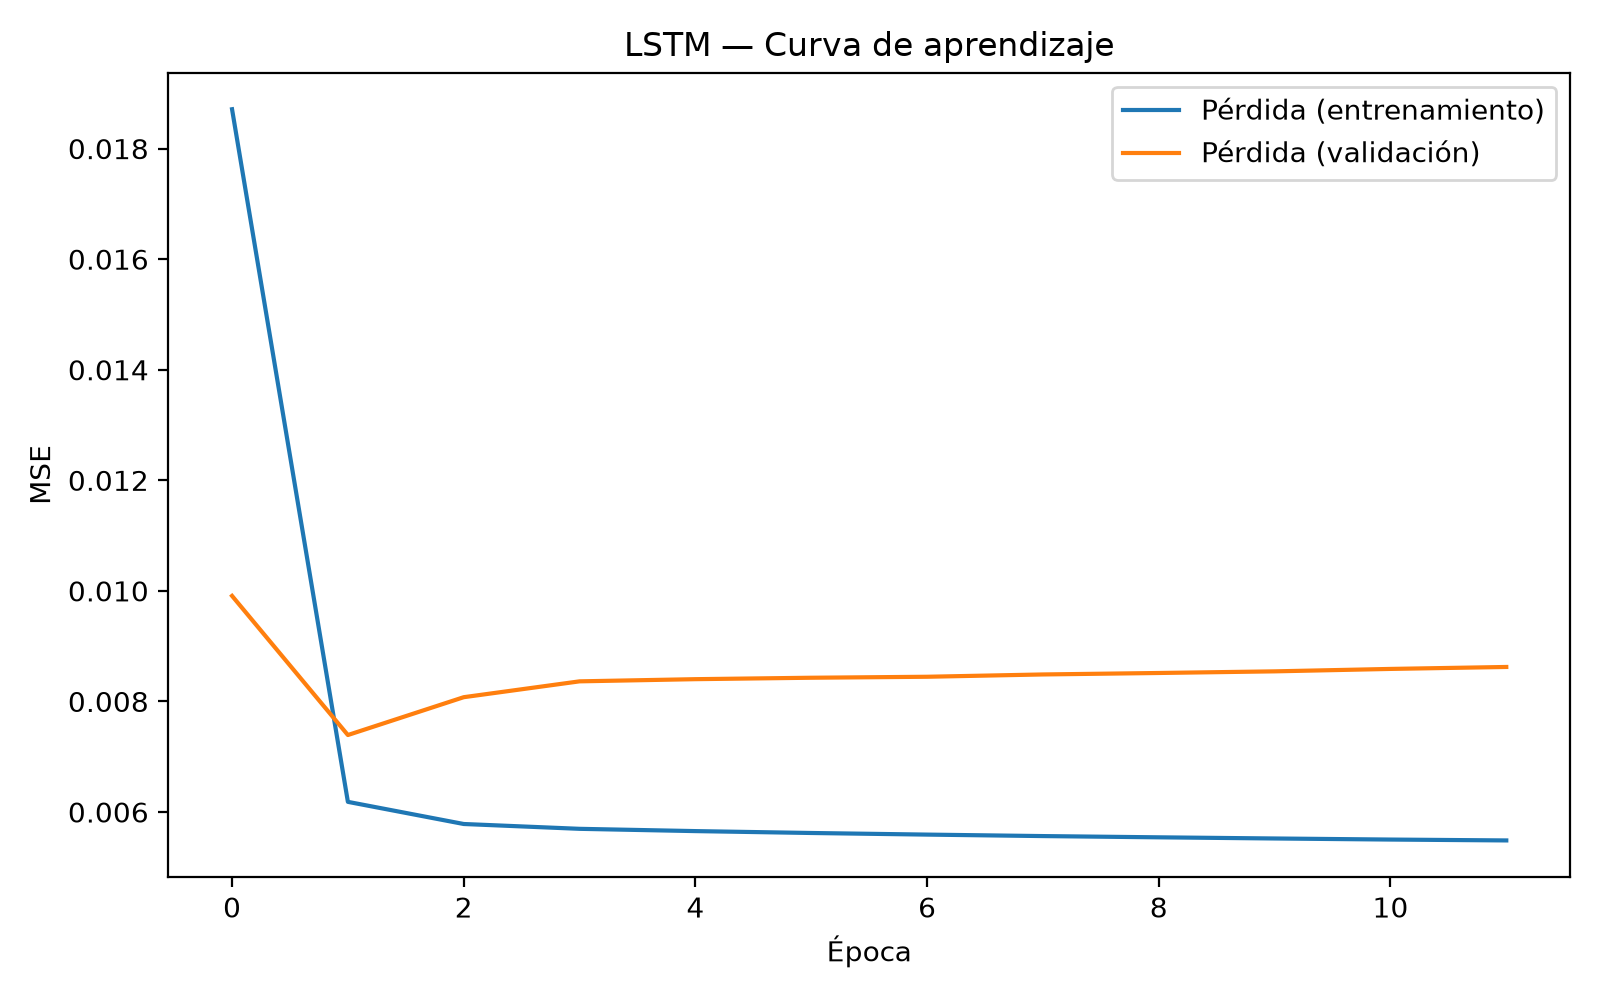
\includegraphics[width=0.75\textwidth]{lstm_curva_aprendizaje.png}
    \caption{Curva de aprendizaje de la red LSTM (pérdida MSE por época), \textit{dataset} piloto MAWI.}
    \label{fig:lstm_curva}
\end{figure}

En el \textit{dataset} primario, la red se reentrenó con la misma arquitectura sobre 46\,582 secuencias y se detuvo en la época 16. La Figura \ref{fig:lstm_primario_curva} muestra una asimetría llamativa: la pérdida de entrenamiento (línea azul) baja de 0.010 a cerca de 0.006, mientras que la de validación (línea naranja discontinua) es prácticamente nula desde la primera época.

\begin{figure}[H]
    \centering
    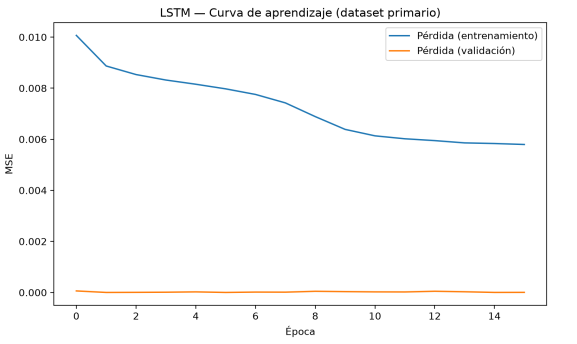
\includegraphics[width=0.75\textwidth]{lstm_primario_curva_aprendizaje.png}
    \caption{Curva de aprendizaje de la red LSTM, \textit{dataset} primario. La separación entre curvas refleja la composición de las particiones: entrenamiento con eventos sintéticos (azul) y validación con tráfico real ocioso (naranja).}
    \label{fig:lstm_primario_curva}
\end{figure}

Esta separación no indica una fuga de datos, sino la composición de las particiones definida en la Sección \ref{sec:obtencion_exploracion}. El entrenamiento incluye los 126 eventos sintéticos, con valores cercanos a 1, mientras que la validación de regresión es 100\,\% tráfico real ocioso, con un máximo normalizado de 0.0029 (Tabla \ref{tab:rangos_normalizados}). Sobre esa partición, el MSE de una predicción cercana a cero es mínimo. Por ello, la distancia entre ambas curvas no sirve por sí sola como indicador de sobreajuste. La pérdida de entrenamiento se estabiliza en torno a 0.006 (RMSE aproximado de 0.077), lo que indica que la red no ajusta por completo los eventos sintéticos ni siquiera en la partición que ve durante el entrenamiento.

La Figura \ref{fig:lstm_primario_curva_split} separa ambas curvas en ejes independientes. En el panel de validación se observa una dinámica del orden de $10^{-4}$: el mínimo se alcanza en la época 1 (línea vertical discontinua) y, a partir de la época 2, la pérdida aumenta hacia $4.0 \times 10^{-4}$. La detención temprana identifica ese deterioro y restaura los pesos de la época 1.
% VERIFICAR: con paciencia 10, detenerse en la época 16 implica un mejor modelo en la época 6, no en la 1.

\begin{figure}[H]
    \centering
    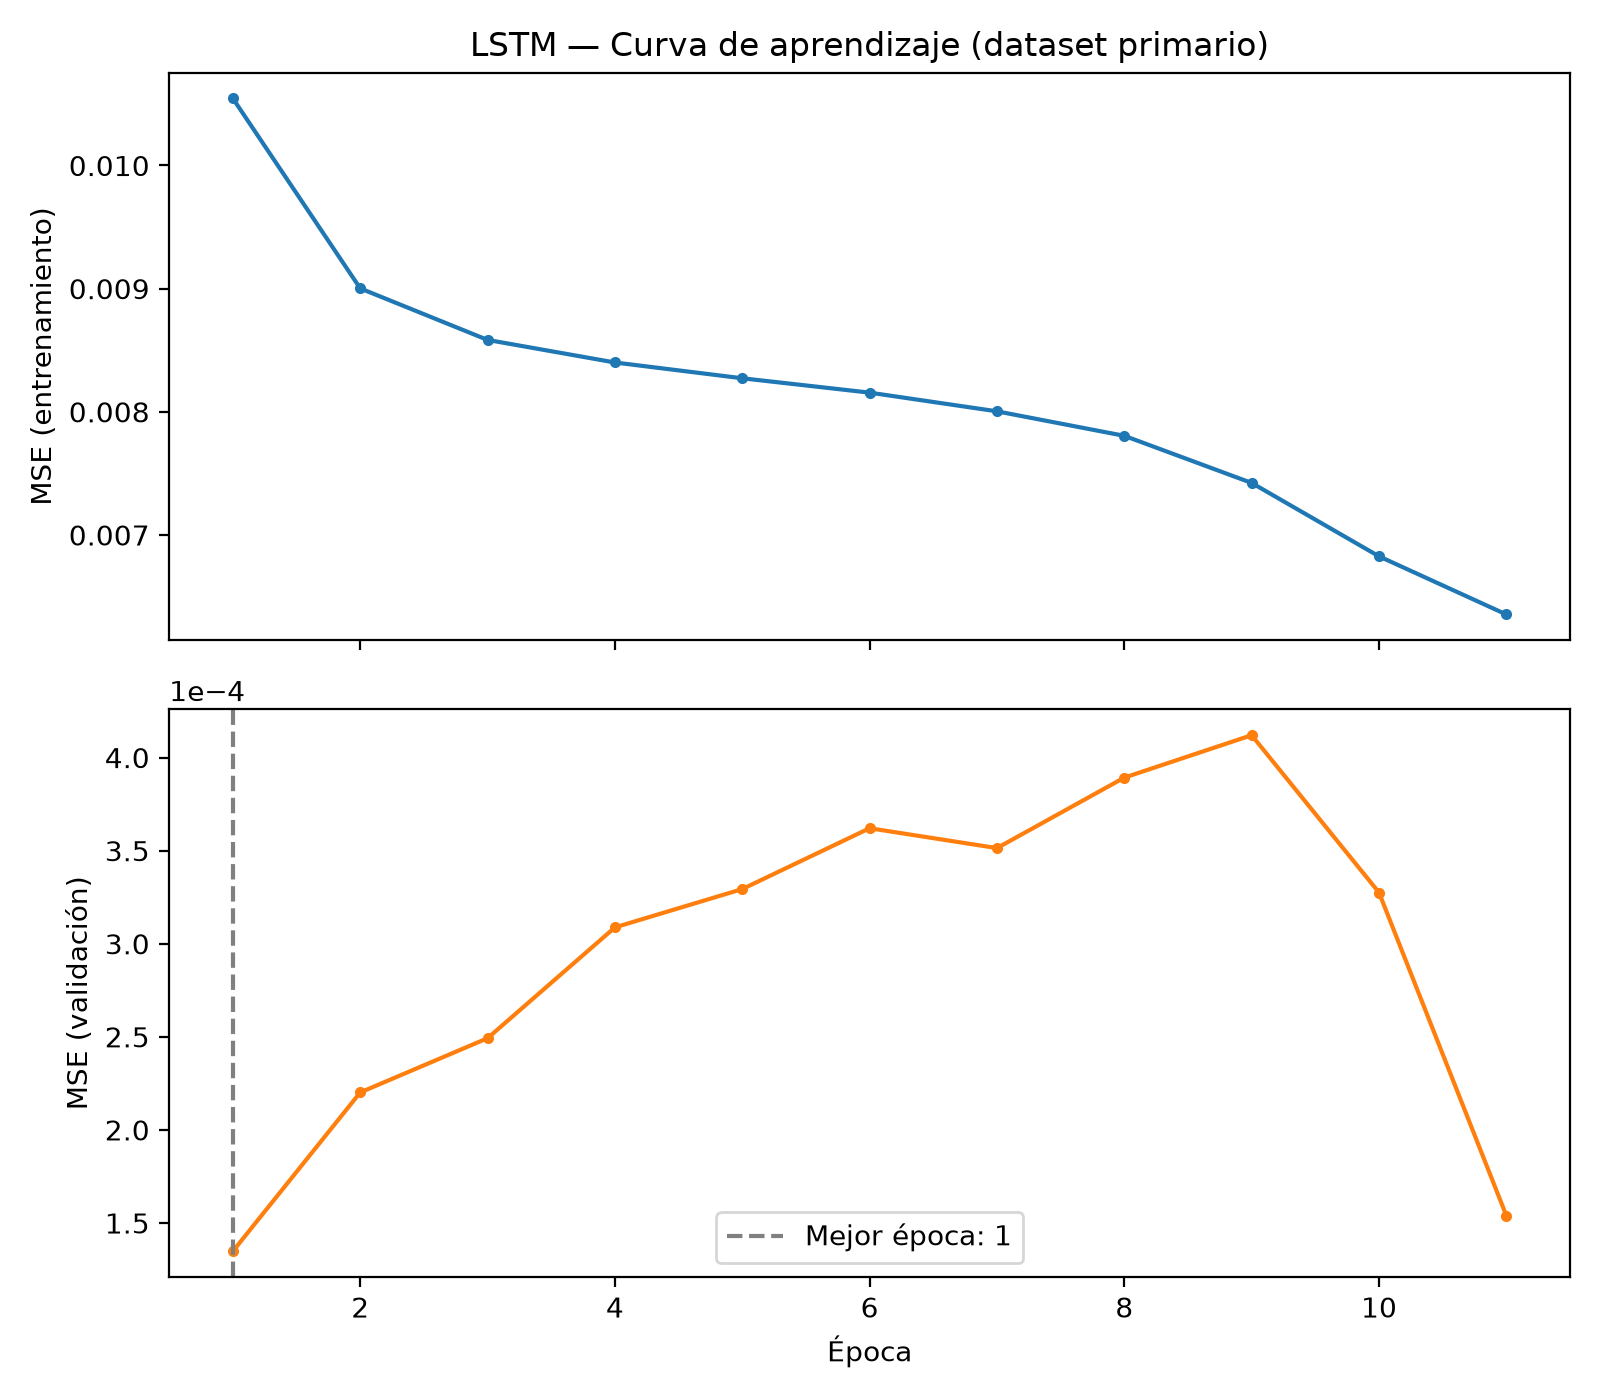
\includegraphics[width=\textwidth]{lstm_primario_curva_aprendizaje1.png}
    \caption{Curva de aprendizaje en ejes independientes. Se aprecia la dinámica de validación en el orden de $10^{-4}$ y el punto de corte de la detención temprana.}
    \label{fig:lstm_primario_curva_split}
\end{figure}

La Figura \ref{fig:lstm_primario_curva_log} unifica ambas curvas en escala logarítmica. Confirma una brecha de aproximadamente dos órdenes de magnitud entre entrenamiento ($\sim 10^{-2}$) y validación ($\sim 10^{-4}$), y muestra que ninguna de las curvas diverge a lo largo del entrenamiento.

\begin{figure}[H]
    \centering
    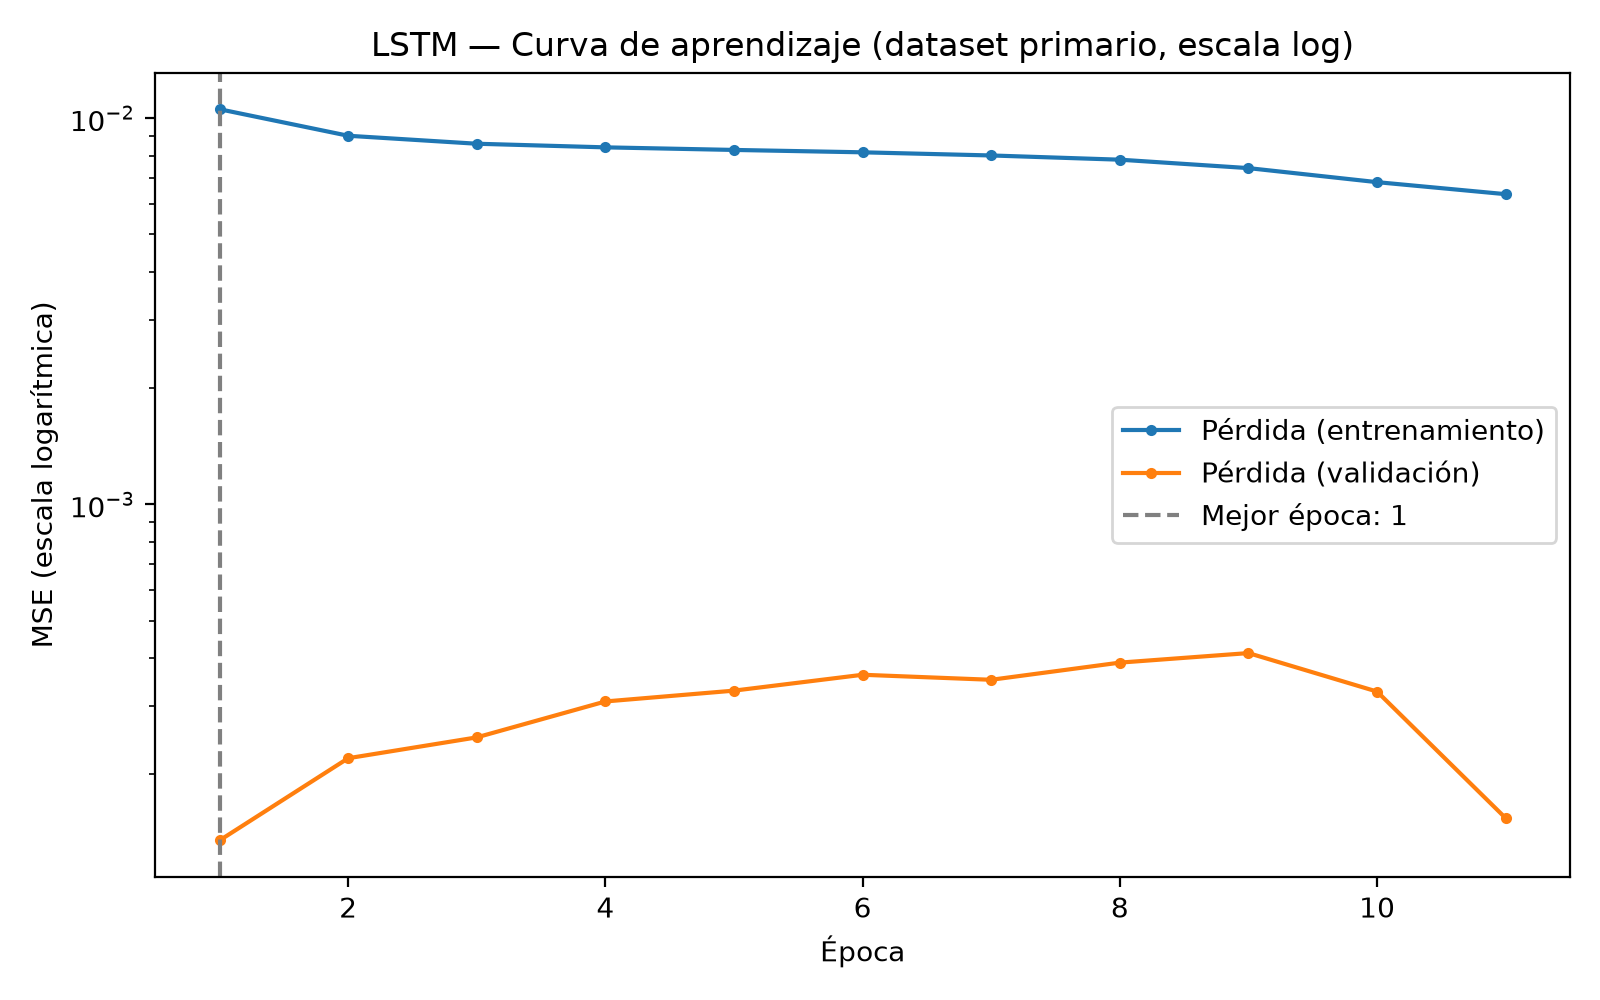
\includegraphics[width=0.85\textwidth]{lstm_primario_curva_aprendizaje_log.png}
    \caption{Curva de aprendizaje de la red LSTM en escala logarítmica, \textit{dataset} primario.}
    \label{fig:lstm_primario_curva_log}
\end{figure}

\subsection*{Fase piloto: regresión}

La Tabla \ref{tab:resultados_lstm_regresion} presenta las métricas sobre MAWI, en escala normalizada.

\begin{table}[H]
    \centering
    \begin{tabular}{|l|r|r|r|}
        \hline
        \textbf{Conjunto} & \textbf{RMSE} & \textbf{MAE} & \textbf{MAPE} \\
        \hline
        Validación & 0.0860 & 0.0664 & 11.53\,\% \\
        Prueba & 0.0891 & 0.0690 & 11.00\,\% \\
        \hline
    \end{tabular}
    \caption{Métricas de regresión de LSTM (escala normalizada), \textit{dataset} piloto MAWI.}
    \label{tab:resultados_lstm_regresion}
\end{table}

El error es estable entre validación y prueba: el RMSE aumenta un 3.6\,\% y el MAPE incluso baja de 11.53\,\% a 11.00\,\%. A diferencia de \textit{Random Forest}, cuyo MAPE pasó de 12.83\,\% a 16.26\,\% (Sección \ref{sec:resultados_rf}), la red no se degrada en la partición de prueba. Respecto al ensamble, el RMSE de prueba baja un 32\,\% (de 0.1311 a 0.0891, ambos normalizados). Frente a ARIMA, que opera en escala original, la comparación exige reescalar: $0.0891 \times 0.306 \approx 0.027$, un valor del mismo orden que el 0.0282 de ARIMA, mientras que el MAPE de ARIMA (10.80\,\%) es ligeramente menor que el de LSTM (11.00\,\%). En regresión sobre el piloto, la red es comparable a la línea base estadística y mejor que el ensamble de árboles.

\begin{figure}[H]
    \centering
    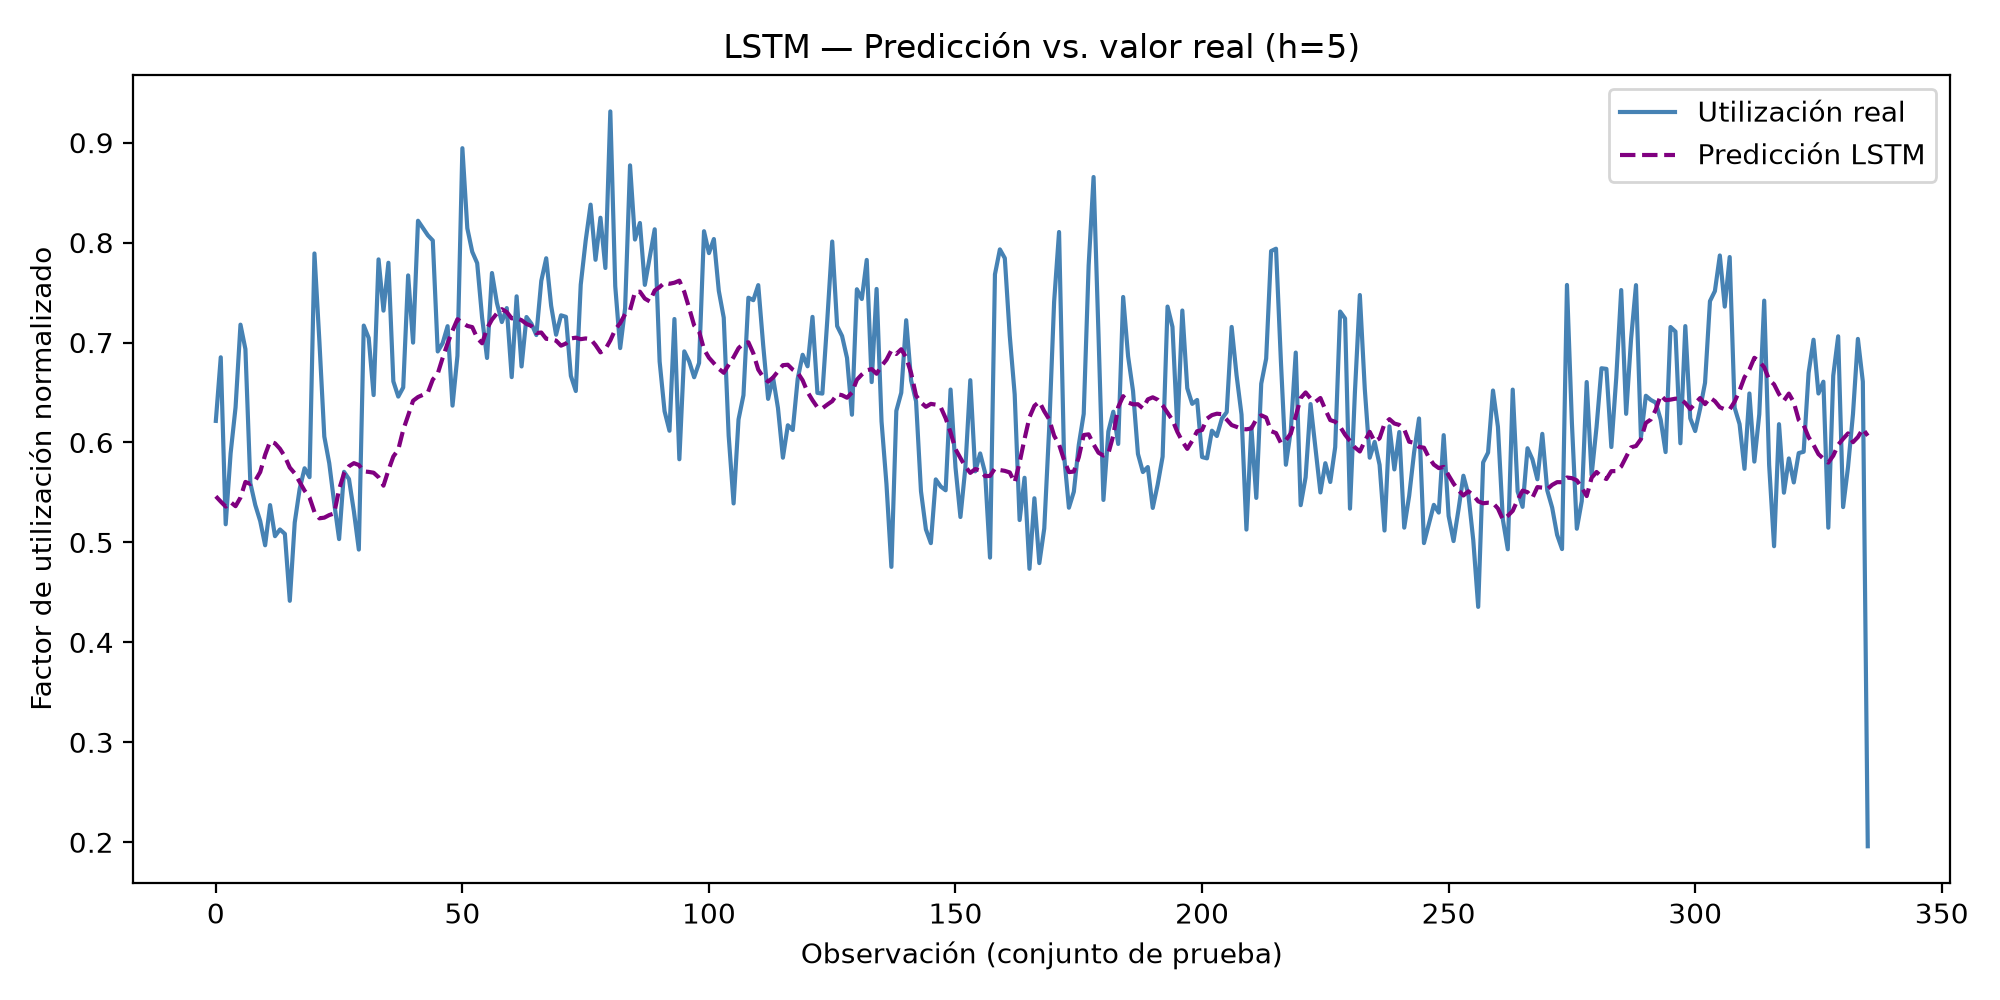
\includegraphics[width=0.85\textwidth]{lstm_prediccion_vs_real.png}
    \caption{LSTM: predicción frente al valor real, partición de prueba del piloto MAWI (escala normalizada).}
    \label{fig:lstm_prediccion}
\end{figure}

La señal real de la Figura \ref{fig:lstm_prediccion} es la misma que la evaluada con \textit{Random Forest}, en escala normalizada; su aspecto distinto de las gráficas de ARIMA se debe a que este operó sobre la métrica sin escalar. La predicción de la red (línea púrpura discontinua) suaviza las oscilaciones de corto plazo y traza la tendencia, como ARIMA. Además, acompaña la caída profunda del final de la serie (cerca de la observación 330), donde el ensamble de árboles se quedaba en un piso. Esa caída está dentro del rango de entrenamiento, por lo que no se trata de extrapolación propiamente dicha, sino de una mejor respuesta a valores poco frecuentes.

\subsection*{Fase piloto: clasificación}

Con el umbral oficial $U_{th}=0.80$ la clasificación no es evaluable en MAWI (Sección \ref{sec:obtencion_exploracion}), por lo que se usó el umbral relativo de prueba $U_{test} \geq 0.25$. La Tabla \ref{tab:resultados_lstm_clasificacion} presenta el desempeño sobre la partición de prueba.

\begin{table}[H]
    \centering
    \begin{tabular}{|l|r|}
        \hline
        \textbf{Métrica ($U_{test} \geq 0.25$)} & \textbf{Prueba} \\
        \hline
        Precisión & 81.2\,\% \\
        \textit{Recall} & 79.4\,\% \\
        \textit{F1-score} & 80.3\,\% \\
        \textbf{Tiempo de Anticipación Efectivo (TAE) promedio} & \textbf{3.9 minutos} \\
        \hline
    \end{tabular}
    \caption{Clasificación y alertamiento (TAE) de LSTM, fase piloto.}
    \label{tab:resultados_lstm_clasificacion}
\end{table}

Cuatro de cada cinco alertas corresponden a un evento real (precisión de 81.2\,\%) y el modelo detecta también cuatro de cada cinco eventos (\textit{recall} de 79.4\,\%). Respecto a ARIMA, el \textit{recall} sube 37.9 puntos porcentuales (de 41.5\,\% a 79.4\,\%) y, respecto a \textit{Random Forest}, 11.1 (de 68.3\,\%). El $TAE$ de 3.9 minutos equivale al 78\,\% del horizonte objetivo de 5 minutos, frente a 2.8 minutos del ensamble y 1.2 de ARIMA. En el piloto, y con un umbral bajo, la red es el mejor detector de los tres. Estas cifras validan el \textit{pipeline}, pero no son comparables con las del \textit{dataset} primario, que usan otro umbral y otros datos.

\subsection*{\textit{Dataset} primario: regresión}

La Tabla \ref{tab:lstm_primario_regresion} presenta las métricas sobre las particiones reales, en escala normalizada.

\begin{table}[H]
    \centering
    \begin{tabular}{|l|r|r|}
        \hline
        \textbf{Conjunto} & \textbf{RMSE} & \textbf{MAE} \\
        \hline
        Validación (real) & 0.000131 & 0.000019 \\
        Prueba (real) & 0.001036 & 0.000125 \\
        \hline
    \end{tabular}
    \caption{Métricas de regresión de LSTM, \textit{dataset} primario (escala normalizada).}
    \label{tab:lstm_primario_regresion}
\end{table}

El RMSE de prueba (0.001036) es unas 44 veces menor que el de ARIMA (0.0459) y unas 48 veces menor que el de \textit{Random Forest} (0.0496) sobre las mismas particiones, y el MAE (0.000125) es unas 120 veces menor que el de ARIMA (0.0151). Como el rango de entrenamiento es cercano a $[0,1]$, la escala normalizada es aproximadamente equivalente a la original, de modo que la comparación es razonable. El error crece entre validación y prueba (el RMSE se multiplica por 7.9 y el MAE por 6.6), y la relación RMSE/MAE (6.9 en validación y 8.3 en prueba) indica que el error se concentra en pocas desviaciones grandes, no en un desajuste generalizado.

\begin{figure}[H]
    \centering
    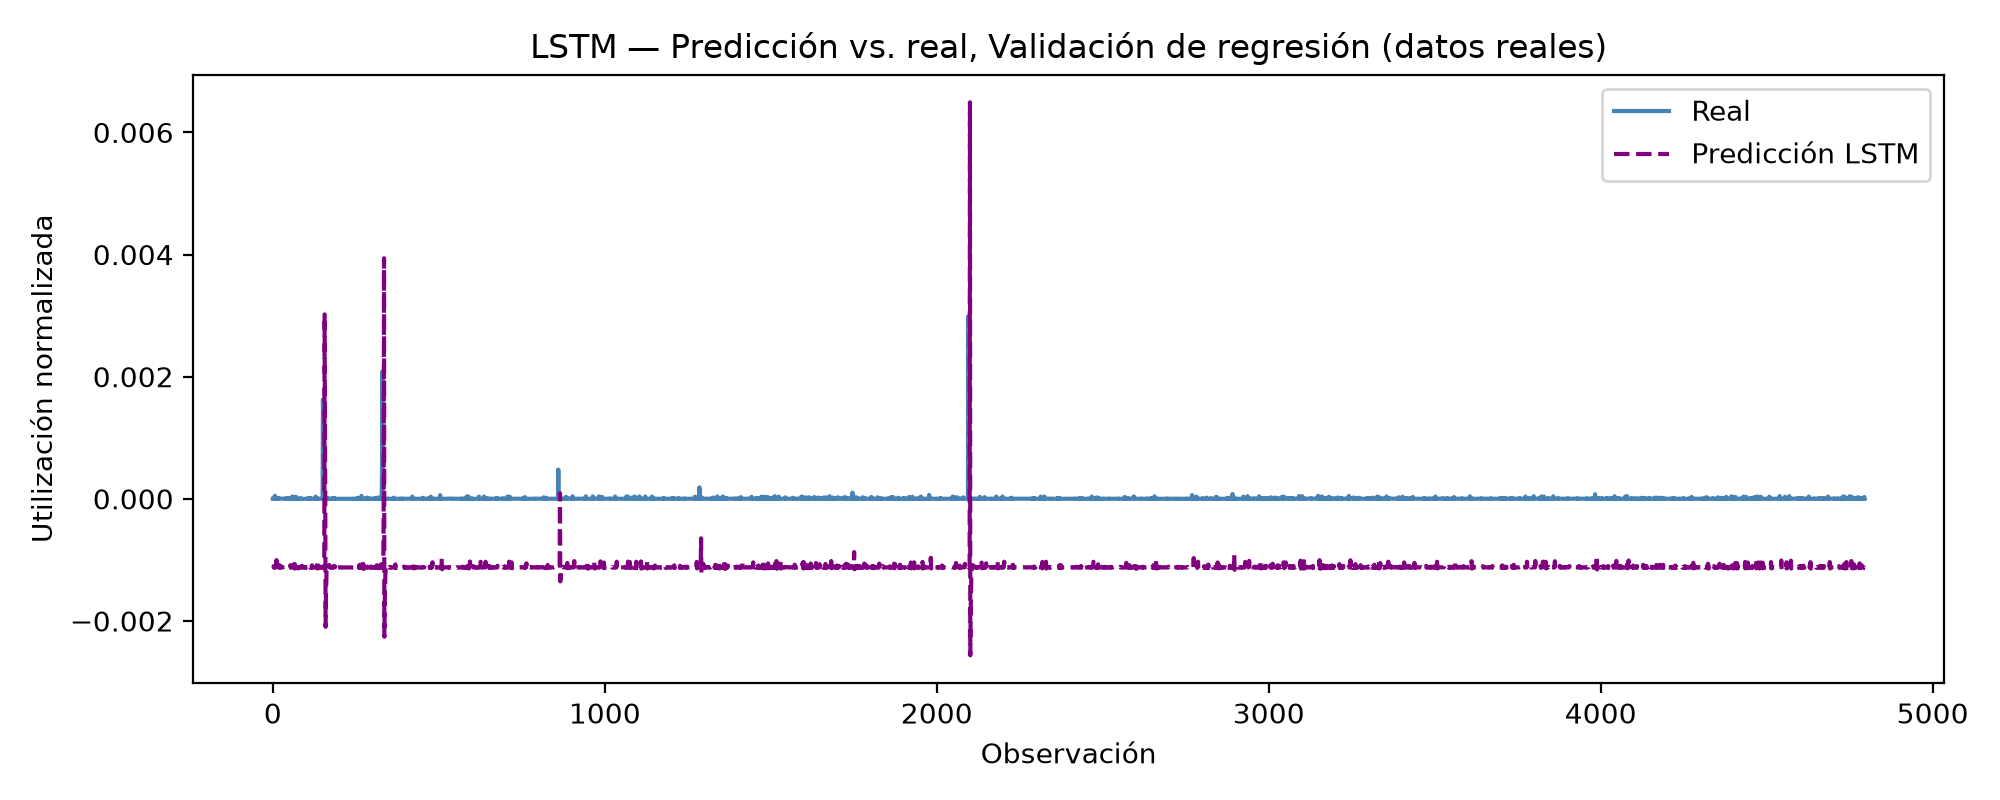
\includegraphics[width=0.85\textwidth]{lstm_primario_regresion_val.png}
    \caption{LSTM: predicción frente al valor real, validación de regresión (\textit{dataset} primario, datos reales).}
    \label{fig:lstm_primario_regresion_val}
\end{figure}

\begin{figure}[H]
    \centering
    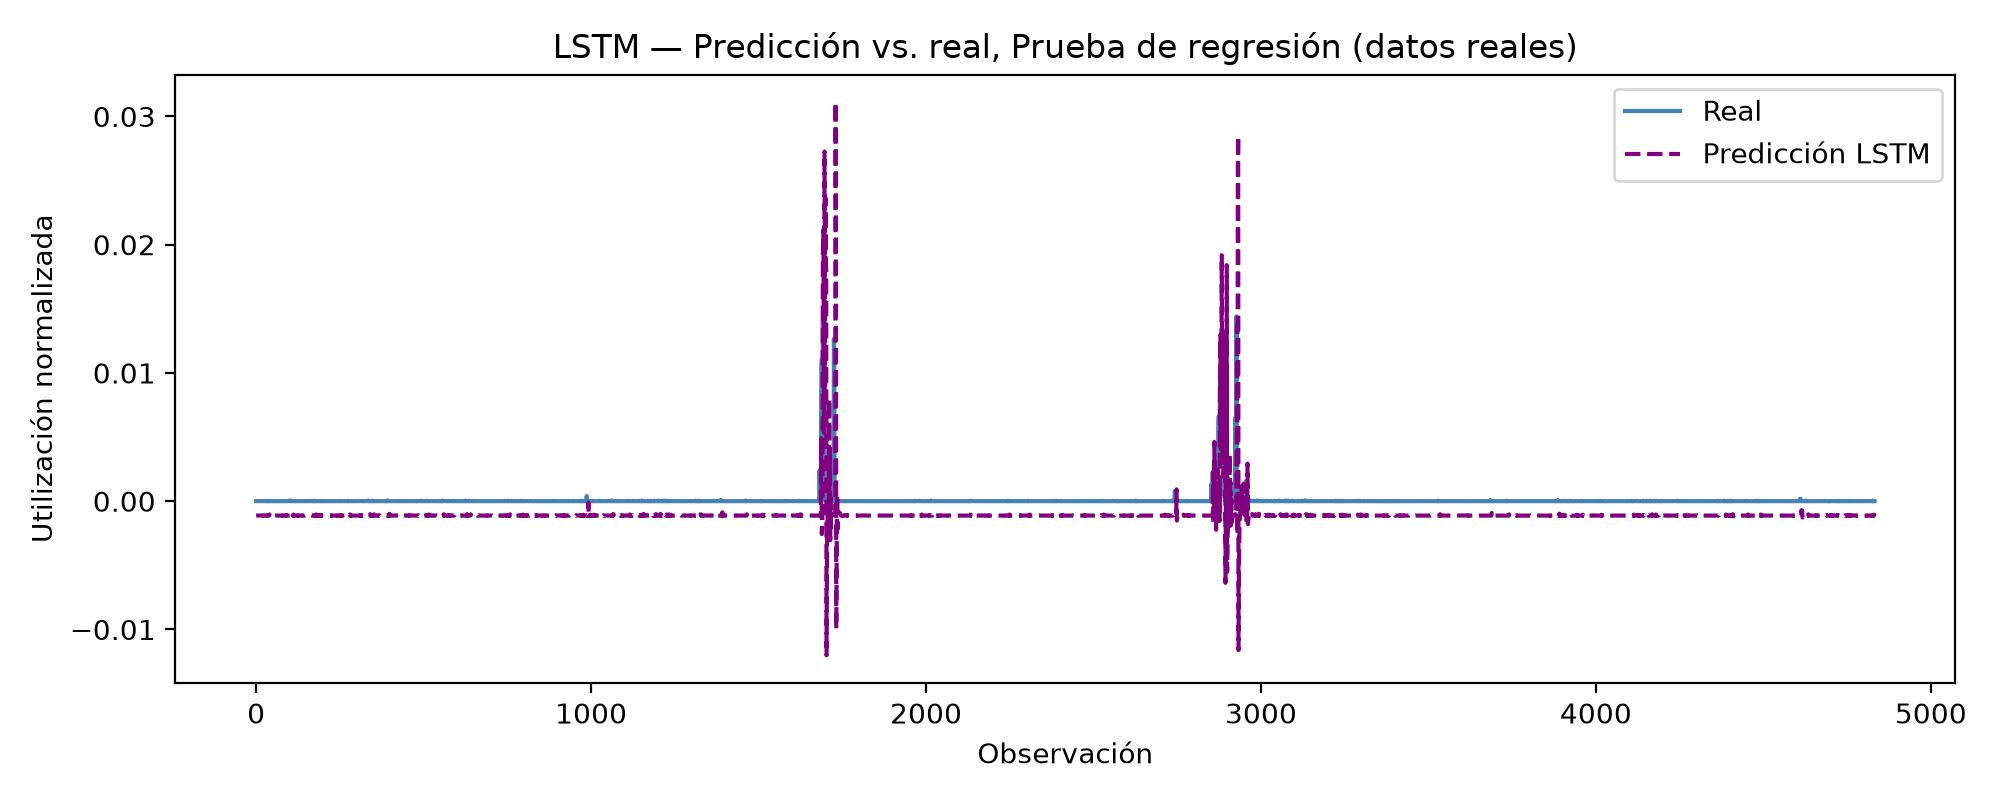
\includegraphics[width=0.85\textwidth]{lstm_primario_regresion_test.png}
    \caption{LSTM: predicción frente al valor real, prueba de regresión (\textit{dataset} primario, datos reales).}
    \label{fig:lstm_primario_regresion_test}
\end{figure}

En validación (Figura \ref{fig:lstm_primario_regresion_val}), la predicción se mantiene anclada al cero real, con perturbaciones que no superan 0.006. En prueba (Figura \ref{fig:lstm_primario_regresion_test}) la red también reacciona ante algunas micro-fluctuaciones y genera picos transitorios, pero su magnitud máxima es de aproximadamente 0.03, unas 23 veces menor que los picos de 0.7 de \textit{Random Forest} sobre el mismo conjunto. Esos picos siguen siendo el doble de la utilización real máxima observada (0.0144) y explican el aumento del error en prueba. El sesgo de sobreestimación que afectó a ARIMA no aparece: la predicción base se adhiere a la señal real, con una oscilación leve hacia valores negativos, esperable en una capa de salida lineal sin restricción de rango.

La Figura \ref{fig:lstm_sintesis_rmse} muestra el RMSE de regresión de la red en los cuatro contextos de evaluación, en escala logarítmica, porque los errores del \textit{dataset} primario (del orden de $10^{-3}$ y $10^{-4}$) quedarían indistinguibles del cero en escala lineal junto a los del piloto (del orden de $10^{-1}$). La diferencia entre ambos conjuntos no debe leerse como una mejora de la red, porque son series distintas: el tráfico real del primario es casi nulo (máximo de 1.44\,\%), y cualquier predicción cercana a cero produce errores absolutos pequeños.

\begin{figure}[H]
    \centering
    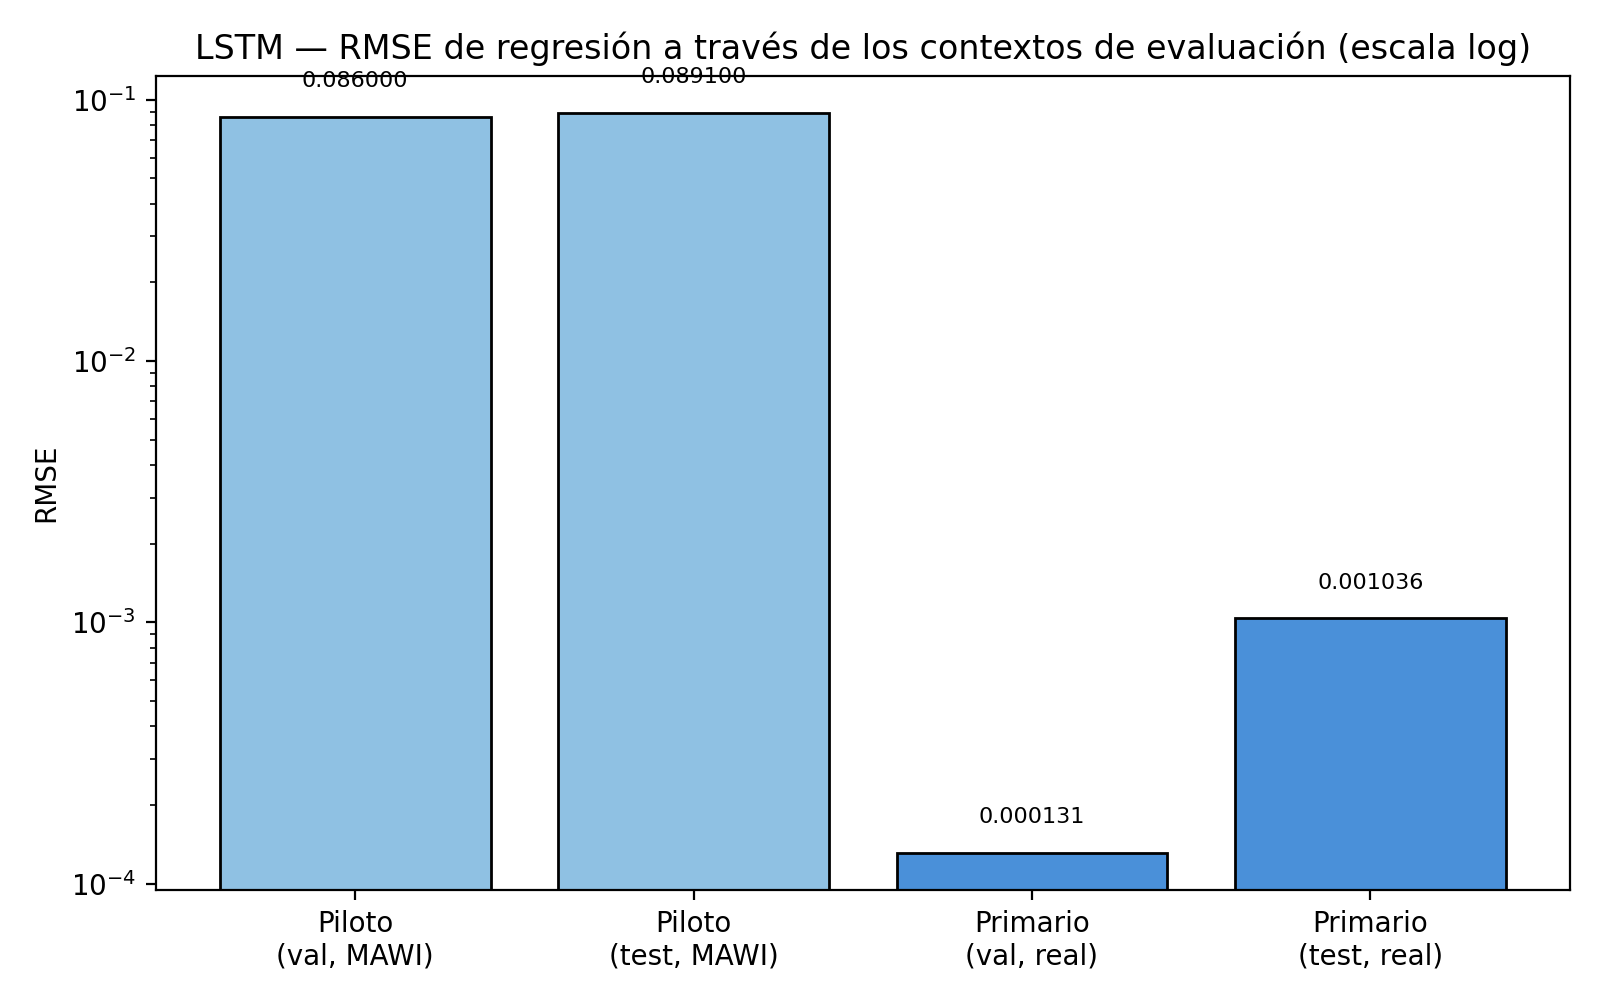
\includegraphics[width=0.85\textwidth]{lstm_sintesis_rmse.png}
    \caption{RMSE de regresión de LSTM en los contextos de evaluación (escala logarítmica).}
    \label{fig:lstm_sintesis_rmse}
\end{figure}

\subsection*{\textit{Dataset} primario: clasificación}

La Tabla \ref{tab:lstm_primario_clasificacion} presenta las métricas de clasificación sobre las particiones sintéticas aisladas, con $U_{th}=0.80$ (en escala normalizada).

\begin{table}[H]
    \centering
    \begin{tabular}{|l|r|r|}
        \hline
        \textbf{Métrica} & \textbf{Validación} & \textbf{Prueba} \\
        \hline
        Exactitud & 0.9742 & 0.9750 \\
        Precisión & 0.7619 & 0.7778 \\
        \textit{Recall} & 0.0563 & 0.0509 \\
        \textit{F1-score} & 0.1049 & 0.0956 \\
        AUC-ROC & 0.8783 & 0.9000 \\
        \hline
    \end{tabular}
    \caption{Métricas de clasificación de LSTM, $U_{th}=0.80$, datos sintéticos aislados.}
    \label{tab:lstm_primario_clasificacion}
\end{table}

El patrón es estable entre ambas particiones. Como en los otros modelos, la exactitud (0.975) tiene poco valor informativo por el desbalance de clases, pues los casos de congestión son cerca del 2.6\,\% de las observaciones. La precisión es aceptable (0.78) y el \textit{recall}, muy bajo (0.051), lo que da un \textit{F1-score} de 0.096. Frente a ARIMA (0.0185), el \textit{recall} es unas 2.8 veces mayor, aunque en términos absolutos sigue siendo muy bajo, y frente a \textit{Random Forest} (0.2982) es unas seis veces menor. El AUC-ROC de 0.90 es alto y casi igual al de los otros dos modelos (0.89 en ARIMA y 0.92 en \textit{Random Forest}).

\begin{figure}[H]
    \centering
    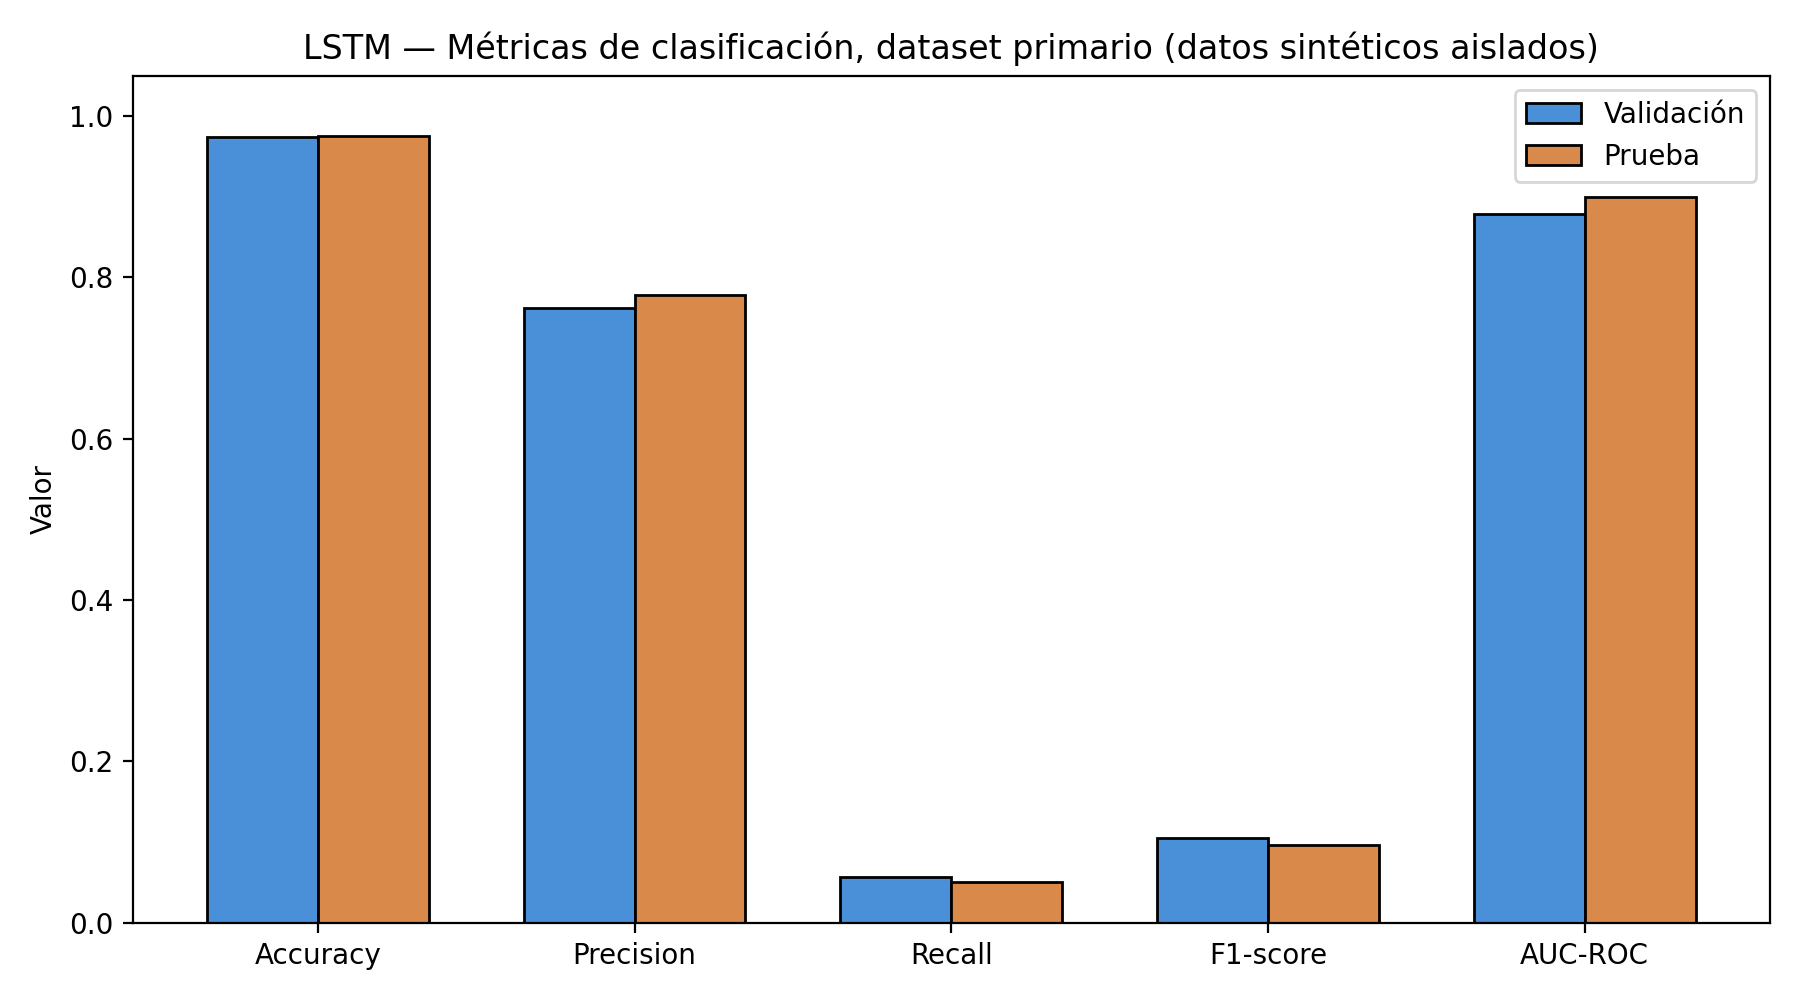
\includegraphics[width=0.8\textwidth]{lstm_sintesis_clasificacion.png}
    \caption{Comparación de métricas de clasificación, validación frente a prueba, LSTM sobre el \textit{dataset} primario.}
    \label{fig:lstm_sintesis_clasificacion}
\end{figure}

La Figura \ref{fig:lstm_sintesis_clasificacion} confirma el patrón: exactitud y AUC-ROC altos, y \textit{recall} y \textit{F1-score} cercanos a cero en ambas particiones. La Ecuación \ref{eq:confusion_lstm} presenta la matriz de confusión sobre la partición de prueba.

\begin{equation}
    \begin{pmatrix} \text{VN}=10\,314 & \text{FP}=4 \\ \text{FN}=261 & \text{VP}=14 \end{pmatrix}
    \label{eq:confusion_lstm}
\end{equation}

Sus componentes se interpretan así:
\begin{itemize}
    \item \textbf{Verdaderos negativos (VN=10\,314):} el modelo reconoce correctamente el tráfico normal, coherente con su buen ajuste del régimen ocioso en regresión.
    \item \textbf{Falsos positivos (FP=4):} la tasa de falsas alarmas es de 0.04\,\% de las observaciones normales, y la precisión es de 77.78\,\% (14 de 18 alertas fueron correctas).
    \item \textbf{Verdaderos positivos (VP=14):} de 275 instantes de congestión, se detectaron 14. Es mucho menos que los 82 de \textit{Random Forest}, aunque más que el único acierto de ARIMA.
    \item \textbf{Falsos negativos (FN=261):} el 94.9\,\% de los instantes de congestión pasa sin alerta.
\end{itemize}

En términos operativos, la red emitió solo 18 alertas en toda la partición. Es un detector casi silencioso: confiable cuando alerta, pero que no avisa en la gran mayoría de las congestiones.

\begin{figure}[H]
    \centering
    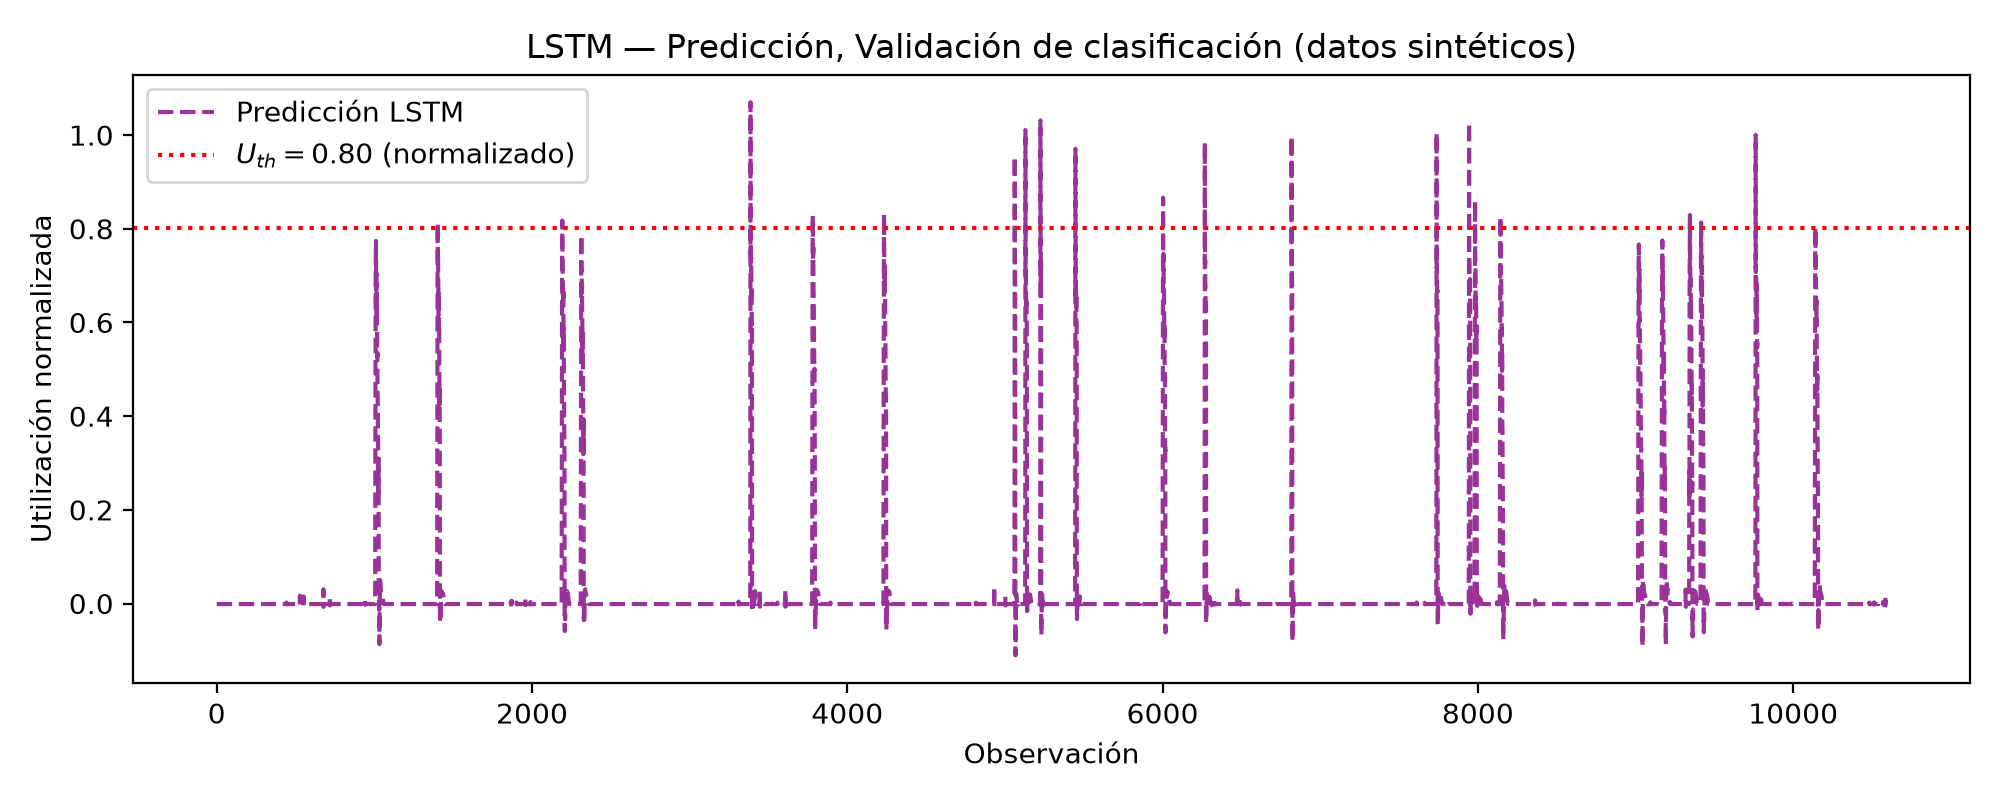
\includegraphics[width=0.85\textwidth]{lstm_primario_clasificacion_val.png}
    \caption{LSTM: predicción frente al valor real y umbral $U_{th}=0.80$, validación de clasificación (\textit{dataset} primario, datos sintéticos aislados).}
    \label{fig:lstm_primario_clasificacion_val}
\end{figure}

\begin{figure}[H]
    \centering
    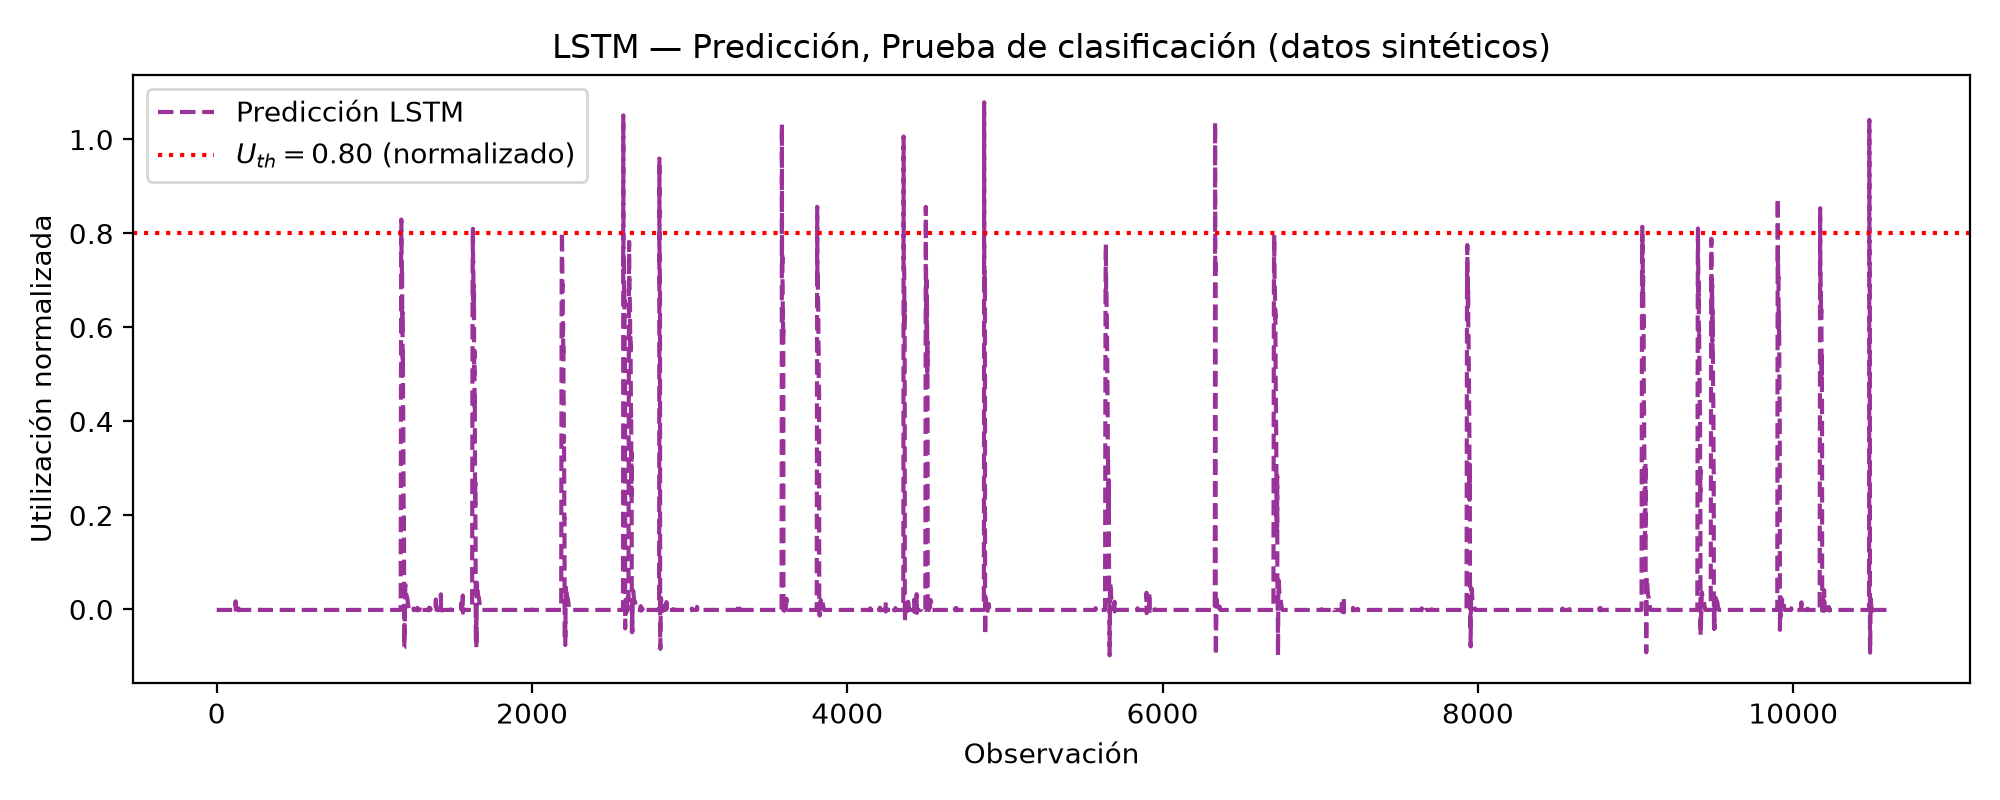
\includegraphics[width=0.85\textwidth]{lstm_primario_clasificacion_test.png}
    \caption{LSTM: predicción frente al valor real y umbral $U_{th}=0.80$, prueba de clasificación (\textit{dataset} primario, datos sintéticos aislados).}
    \label{fig:lstm_primario_clasificacion_test}
\end{figure}

Las Figuras \ref{fig:lstm_primario_clasificacion_val} y \ref{fig:lstm_primario_clasificacion_test} muestran el origen de los falsos negativos. La predicción (línea púrpura discontinua) reacciona ante las anomalías inyectadas y asciende de forma sincronizada con las crisis, pero con magnitud amortiguada: muchos picos se quedan justo por debajo de la línea de alerta (0.80), y solo 14 la cruzan. El patrón es el mismo en validación y en prueba.

La Figura \ref{fig:comparativa_recall} sitúa este resultado frente a los otros dos modelos sobre la misma tarea, y la comparativa completa se desarrolla en la Sección 6.4. La comparación es indicativa, no estricta, porque las matrices de confusión de los modelos no se calcularon sobre el mismo número de observaciones.

\begin{figure}[H]
    \centering
    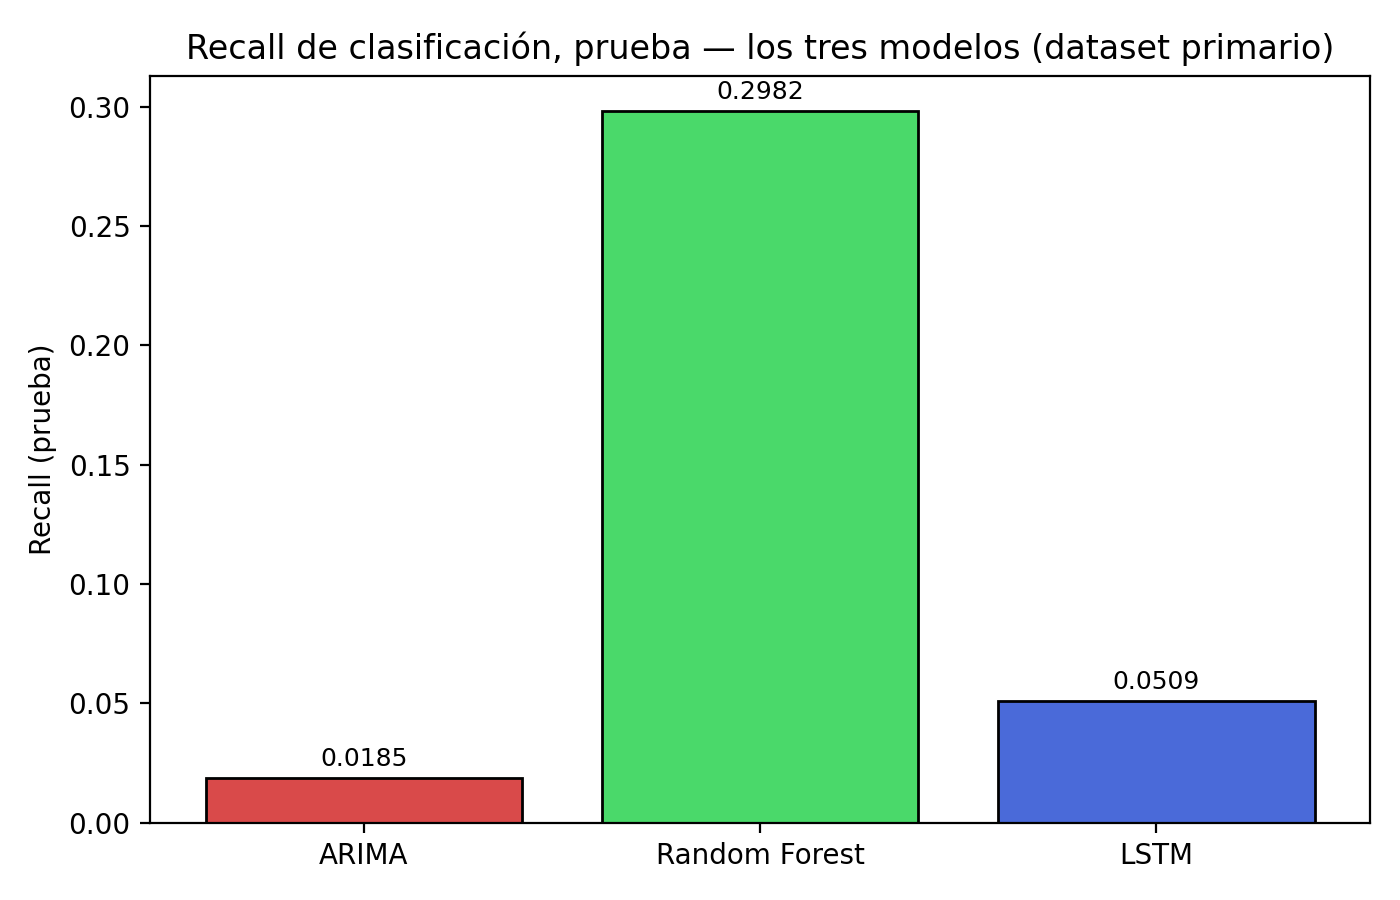
\includegraphics[width=0.7\textwidth]{comparativa_recall_tres_modelos.png}
    \caption{\textit{Recall} de clasificación (prueba) de los tres modelos sobre el \textit{dataset} primario.}
    \label{fig:comparativa_recall}
\end{figure}

\subsection*{Piloto frente a \textit{dataset} primario}

La Tabla \ref{tab:comparativa_lstm_piloto_primario} resume la comparación de la red entre ambas fases.

\begin{table}[H]
    \centering
    \begin{tabular}{|l|r|r|}
        \hline
        \textbf{Métrica (prueba)} & \textbf{Piloto (MAWI)} & \textbf{Primario} \\
        \hline
        Secuencias de entrenamiento & 1\,044 & 46\,582 \\
        Épocas hasta la detención & 12 & 16 \\
        RMSE (regresión, normalizado) & 0.0891 & 0.001036 \\
        \textit{Recall} (clasificación) & 79.4\,\% ($U_{test}=0.25$) & 5.1\,\% ($U_{th}=0.80$) \\
        \textit{F1-score} (clasificación) & 80.3\,\% ($U_{test}=0.25$) & 9.6\,\% ($U_{th}=0.80$) \\
        AUC-ROC (clasificación) & N/A & 0.9000 \\
        \hline
    \end{tabular}
    \caption{Comparación de LSTM entre la fase piloto y el \textit{dataset} primario. Los RMSE corresponden a series distintas y las métricas de clasificación usan umbrales distintos, por lo que no son directamente comparables. N/A: no aplicable con el umbral oficial (Sección \ref{sec:obtencion_exploracion}).}
    \label{tab:comparativa_lstm_piloto_primario}
\end{table}

\subsection*{Validación de generalización no realizada}

Como \textit{Random Forest}, la red no pudo evaluarse sobre MAWI reagregado a la granularidad oficial de 1 minuto. Su ventana de entrada es de $w=30$ pasos (Sección \ref{sec:preprocesamiento}) y exige al menos 30 observaciones consecutivas para generar una predicción, mientras que cada traza de MAWI aporta solo 15 minutos continuos (Sección \ref{sec:obtencion_exploracion}). ARIMA, en cambio, opera sobre la serie continua sin requerir una ventana fija, y por eso sí pudo evaluarse. Acortar la ventana alteraría la configuración validada y haría injusta cualquier comparación, por lo que esta validación se reporta como no realizada.

\subsection*{Síntesis de los resultados de LSTM}

La Tabla \ref{tab:sintesis_completa_lstm} reúne las métricas de todos los contextos de evaluación.

\begin{table}[H]
    \centering
    \small
    \begin{tabular}{|l|l|r|r|r|}
        \hline
        \textbf{Contexto} & \textbf{Naturaleza de los datos} & \textbf{RMSE} & \textbf{\textit{Recall}} & \textbf{AUC-ROC} \\
        \hline
        Piloto --- validación & 100\,\% real (MAWI) & 0.0860 & N/A & N/A \\
        Piloto --- prueba & 100\,\% real (MAWI) & 0.0891 & N/A & N/A \\
        Primario --- regresión (val.) & 100\,\% real & 0.000131 & --- & --- \\
        Primario --- regresión (prueba) & 100\,\% real & 0.001036 & --- & --- \\
        Primario --- clasificación (val.) & 100\,\% sintético & --- & 0.0563 & 0.8783 \\
        Primario --- clasificación (prueba) & 100\,\% sintético & --- & 0.0509 & 0.9000 \\
        Generalización --- MAWI (oficial) & \multicolumn{4}{c|}{No evaluable (incompatibilidad estructural)} \\
        \hline
    \end{tabular}
    \caption{Síntesis de los resultados de LSTM. N/A: no aplicable con el umbral oficial (Sección \ref{sec:obtencion_exploracion}). Los RMSE están en escala normalizada.}
    \label{tab:sintesis_completa_lstm}
\end{table}

\subsection*{Discusión de los resultados de LSTM}

\textbf{Regresión.} Sobre el \textit{dataset} primario, la red obtiene el menor error de los tres modelos, con una diferencia de dos órdenes de magnitud en el MAE y de más de uno en el RMSE. Esa ventaja debe leerse con cautela. El tráfico real es casi nulo (media de $2.2 \times 10^{-5}$ y desviación estándar de $3.5 \times 10^{-4}$ en fracción, Tabla \ref{tab:estadisticas_real}), de modo que cualquier predicción pegada a cero tiene un error pequeño. ARIMA y \textit{Random Forest} quedan muy por detrás sobre todo porque presentan sesgo de sobreestimación y picos espurios, respectivamente, no porque la red capte una dinámica que los otros ignoran. Para sustentar una ventaja predictiva real habría que compararla con una línea base ingenua (por ejemplo, repetir el último valor o predecir la media), que no se evaluó en este trabajo. De hecho, el RMSE de prueba (0.001036) es aproximadamente tres veces la desviación estándar de toda la serie real, lo que muestra el peso de los pocos picos espurios, aunque la red los limita mucho más que los otros modelos. Una explicación plausible es que el estado interno de la red atenúa las fluctuaciones aisladas, pero con estos datos no puede demostrarse.

\textbf{Piloto.} En el piloto la red es comparable a ARIMA en regresión (RMSE reescalado de 0.027 frente a 0.0282, y MAPE de 11.00\,\% frente a 10.80\,\%) y mejor que \textit{Random Forest}. Su mayor fortaleza está en la clasificación con umbral bajo: \textit{recall} de 79.4\,\% y $TAE$ de 3.9 minutos, el mejor de los tres modelos. Estas cifras, sin embargo, se obtienen con $U_{test}=0.25$ sobre otra serie, y no anticipan el comportamiento con el umbral oficial.

\textbf{Clasificación en el primario.} El resultado contrasta con el piloto: el \textit{recall} cae a 5.1\,\%, menor que el del ensamble de árboles. Varias causas, no excluyentes, podrían explicarlo. La primera es la función de pérdida: al minimizar el MSE sobre un entrenamiento con el 97.9\,\% de las observaciones por debajo del umbral (Sección \ref{sec:obtencion_exploracion}), el error global se reduce sobre todo prediciendo bien el régimen mayoritario, y la curva de entrenamiento, que se estabiliza en 0.006, sugiere que los eventos quedan ajustados solo en parte. La segunda es el criterio de detención temprana, que se guía por la validación de regresión (100\,\% tráfico real ocioso): conserva los pesos que mejor predicen el tráfico ocioso, no los que mejor detectan congestión, y la curva sugiere que esos pesos son los de una etapa muy temprana del entrenamiento. La tercera es la distancia entre la magnitud predicha y el umbral fijo de 0.80, evidente en las Figuras \ref{fig:lstm_primario_clasificacion_val} y \ref{fig:lstm_primario_clasificacion_test}. Con los experimentos realizados no se puede aislar cuánto aporta cada una.

\textbf{Umbral frente a señal.} El AUC-ROC de la red (0.90) es casi idéntico al de ARIMA (0.89) y al de \textit{Random Forest} (0.92), a pesar de que sus \textit{recall} difieren en más de un orden de magnitud. Esto indica que las tres predicciones continuas ordenan de forma parecida los instantes de congestión por encima de los normales, y que la diferencia en \textit{recall} proviene sobre todo de la amplitud de las predicciones frente al umbral fijo. Por tanto, la calibración del umbral sobre la partición de validación, o una función de pérdida que pondere los eventos, son vías para mejorar la detección que este trabajo no exploró. Con un desbalance tan fuerte, convendría además complementar el AUC-ROC con una curva precisión-\textit{recall}.

\textbf{Generalización.} La imposibilidad de evaluar la red sobre MAWI, igual que en \textit{Random Forest}, tiene origen en la ventana de entrada de 30 pasos frente a trazas de 15 minutos. Es una consecuencia de la configuración elegida y no una propiedad de los algoritmos, pero limita la comparación con ARIMA, que fue el único modelo evaluable en este escenario.

\textbf{Alcance.} En conjunto, la red ajusta mejor que los otros modelos el tráfico real ocioso, con picos espurios muy acotados, pero con el umbral oficial detecta menos congestión que \textit{Random Forest}. Estas conclusiones se integran con las de los otros modelos en las Secciones 6.4 y 6.5.










\section{Comparativa de modelos}
\label{sec:comparativa_modelos}

Las Secciones \ref{sec:resultados_arima} a \ref{sec:resultados_lstm} presentaron, de manera individual, los resultados de cada modelo a través de los distintos contextos de evaluación de esta investigación. Esta sección integra dichos resultados en una comparativa transversal orientada a responder directamente la pregunta que subyace al diseño experimental completo de este trabajo (Sección \ref{sec:modelos_justificacion}): ¿existe un modelo que domine de manera uniforme sobre los demás, o el desempeño relativo depende de 
la tarea, del conjunto de datos y de las condiciones de evaluación?

\subsection*{Tabla maestra de resultados}

La Tabla \ref{tab:tabla_maestra} consolida, en un solo lugar, la totalidad de las métricas cuantitativas obtenidas por los tres modelos a lo largo de este trabajo.

\begin{table}[H]
    \centering
    \small
    \begin{tabular}{|l|l|r|r|r|}
        \hline
        \textbf{Contexto} & \textbf{Modelo} & \textbf{RMSE} & \textbf{\textit{Recall}} & \textbf{AUC-ROC} \\
        \hline
        \multirow{3}{*}{Piloto --- prueba (MAWI, 100\,\% real)}
            & ARIMA & 0.0282 & N/A & N/A \\
            & \textit{Random Forest} & 0.1311 & N/A & N/A \\
            & LSTM & 0.0891 & N/A & N/A \\
        \hline
        \multirow{3}{*}{Primario --- regresión, prueba (100\,\% real)}
            & ARIMA & 0.0459 & --- & --- \\
            & \textit{Random Forest} & 0.0496 & --- & --- \\
            & LSTM & \textbf{0.0010} & --- & --- \\
        \hline
        \multirow{3}{*}{Primario --- clasificación, prueba (100\,\% sintético)}
            & ARIMA & --- & 0.0185 & 0.8939 \\
            & \textit{Random Forest} & --- & \textbf{0.2982} & 0.9187 \\
            & LSTM & --- & 0.0509 & 0.9000 \\
        \hline
        \multirow{3}{*}{Generalización --- MAWI, 1 min (100\,\% real)}
            & ARIMA & 0.3233 & N/A & N/A \\
            & \textit{Random Forest} & \multicolumn{3}{c|}{No evaluable} \\
            & LSTM & \multicolumn{3}{c|}{No evaluable} \\
        \hline
    \end{tabular}
    \caption{Tabla maestra: totalidad de resultados cuantitativos de los tres modelos evaluados en esta tesis.}
    \label{tab:tabla_maestra}
\end{table}

Un primer examen de esta tabla revela un patrón que se sostiene consistentemente a través de todos los conjuntos de prueba: \textbf{ningún modelo domina de manera uniforme ambas tareas}. LSTM es superior por un margen abrumador en regresión; \textit{Random Forest} es superior, también por un margen considerable, en clasificación binarizada; y ARIMA, la línea base estadística, ocupa consistentemente el último lugar en ambas dimensiones ---cumpliendo, en ese sentido, precisamente la función de referencia mínima para la que 
fue concebido en la metodología (Sección \ref{sec:modelos_justificacion})---.

\subsection*{El \textit{trade-off} central: precisión continua vs. sensibilidad de alertamiento}

La conclusión fundamental de esta investigación no reside en la declaración de un modelo victorioso absoluto, sino en la demostración matemática de una paradoja intrínseca al pronóstico de series de tiempo de red. La Figura \ref{fig:scatter_tradeoff} visualiza este hallazgo ---el \textit{trade-off} algorítmico--- de la manera más directa posible: cada modelo se posiciona en un plano cartesiano cuyo eje horizontal representa su error continuo de regresión (RMSE, donde menor es mejor, en escala logarítmica) y cuyo eje vertical representa su sensibilidad operativa de clasificación (\textit{Recall}, donde mayor es mejor).

\begin{figure}[H]
    \centering
    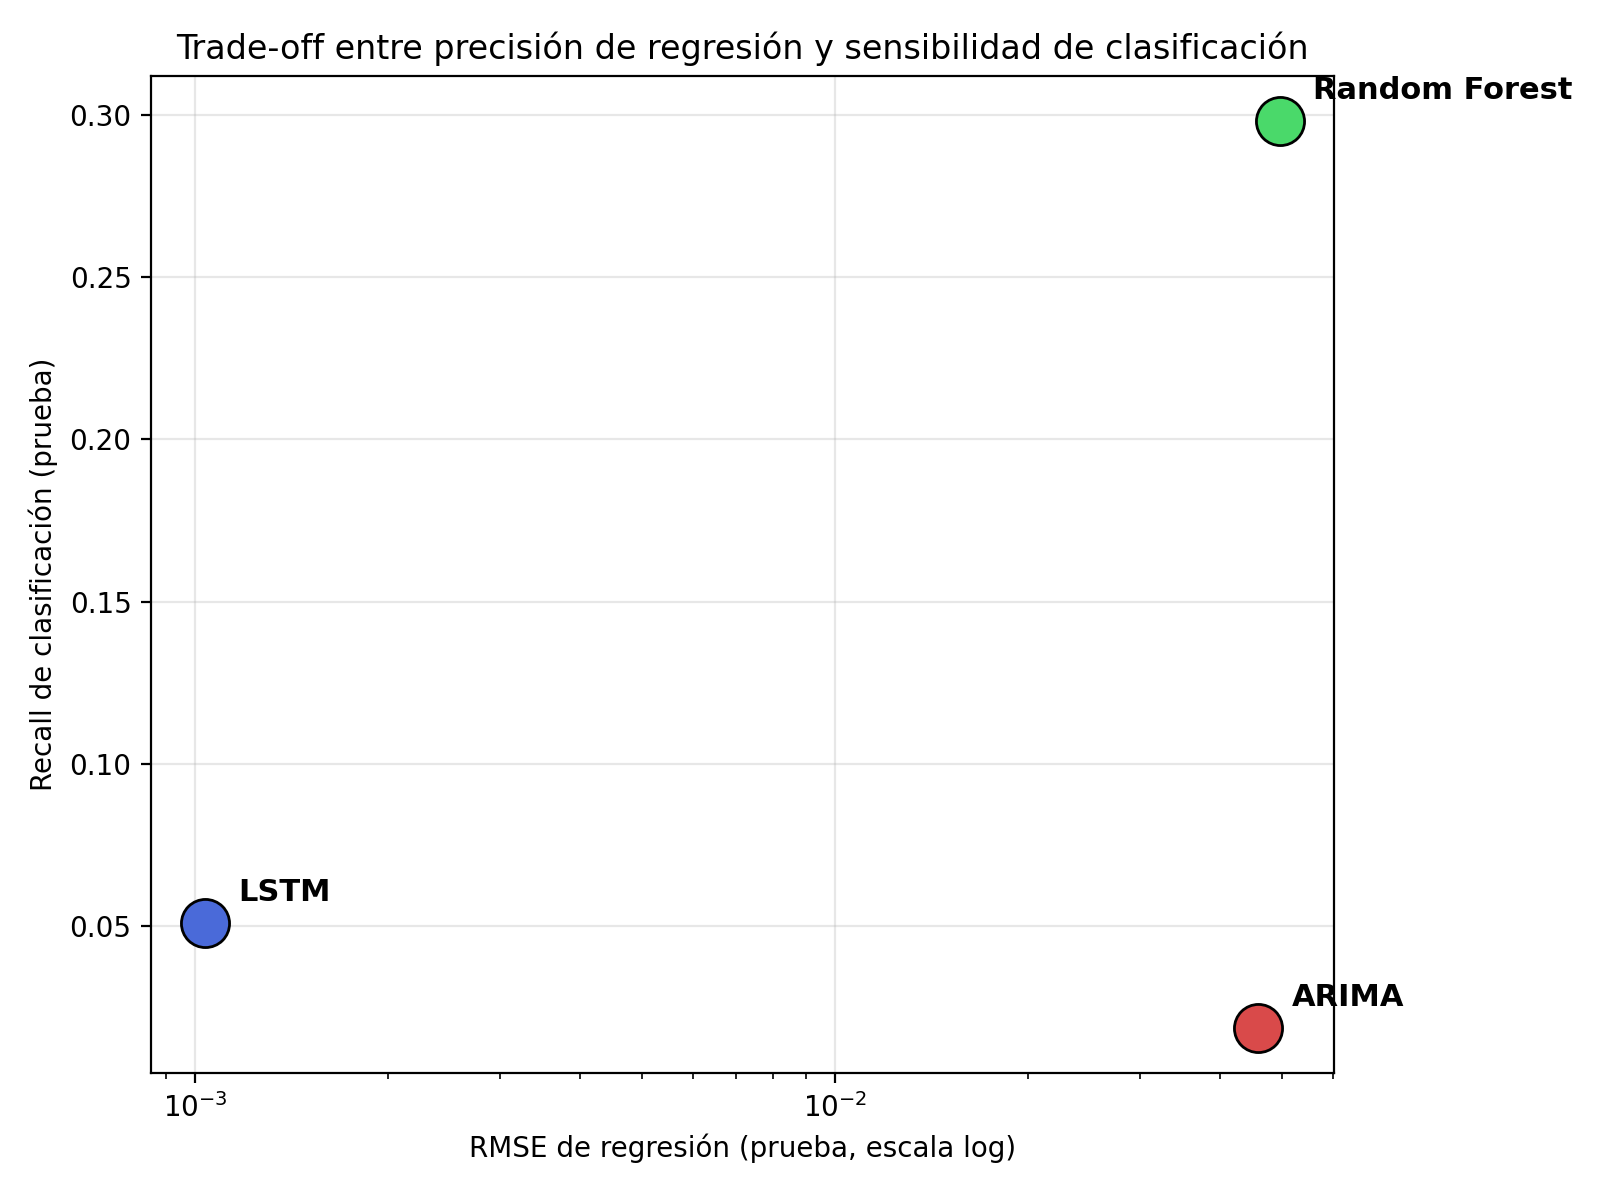
\includegraphics[width=0.75\textwidth]{scatter_tradeoff_rmse_recall.png}
    \caption{\textit{Trade-off} algorítmico: Precisión basal (RMSE, eje X) vs. Sensibilidad de detección (\textit{Recall}, eje Y). Ningún modelo logra la dominancia absoluta en el plano cartesiano.}
    \label{fig:scatter_tradeoff}
\end{figure}

La distribución espacial de los nodos en la gráfica revela el perfil de especialización de cada arquitectura:
\begin{itemize}
    \item \textbf{El dominio del letargo (LSTM, punto azul):} La red neuronal recurrente se sitúa en el extremo izquierdo del plano, presumiendo un RMSE microscópico ($10^{-3}$). Sin embargo, su posición inferior en el eje Y confirma que el costo matemático de lograr una estabilidad perfecta durante el tráfico ocioso fue desarrollar una severa ceguera conservadora (bajo \textit{Recall}) frente a las crisis anómalas repentinas.
    \item \textbf{La hiper-vigilancia reactiva (\textit{Random Forest}, punto verde):} El ensamble de árboles corona el eje vertical, ostentando la mayor agudeza para detectar instantes genuinos de congestión (\textit{Recall} máximo). No obstante, su desplazamiento hacia la derecha del plano evidencia el daño colateral: su hipersensibilidad a las anomalías fracturó su capacidad para predecir el flujo basal, resultando en un error continuo (RMSE) elevado producto de constantes alucinaciones predictivas.
    \item \textbf{La inoperancia asimétrica (ARIMA, punto rojo):} El modelo estadístico tradicional queda relegado a la zona de peor rendimiento (esquina inferior derecha). Su rigidez paramétrica le impidió tanto rastrear el flujo basal con precisión (alto RMSE) como detectar las ráfagas agudas (bajo \textit{Recall}), confirmando su obsolescencia para topologías de red volátiles.
\end{itemize}

Si existiera un algoritmo totalmente eficiente en todo sentido para la ingeniería de tráfico, su nodo se ubicaría en la esquina superior izquierda (RMSE cero y \textit{Recall} absoluto). La disposición geométrica evidenciada ---tres arquitecturas ocupando clústeres especializados y diametralmente opuestos--- constituye la prueba definitiva del hallazgo central de la tesis: en entornos de red masivamente asimétricos, la optimización para el pronóstico continuo (\textit{Smoothness}) y la optimización para la detección de anomalías (\textit{Sharpness}) son objetivos matemáticamente contrapuestos. No existe un modelo universal; la elección del algoritmo debe estar dictada estrictamente por el objetivo del administrador de la red.

\subsection*{Comparación multidimensional}

La Figura \ref{fig:radar_comparativo} amplía la evaluación comparativa a un espacio de cinco dimensiones simultáneas: capacidad de regresión (invertida y normalizada, donde un valor periférico indica un error RMSE cercano a cero), Precisión, \textit{Recall}, \textit{F1-score} y AUC-ROC. Esta representación geométrica permite auditar el perfil de fortalezas y debilidades estructurales de cada arquitectura de un solo vistazo.

\begin{figure}[H]
    \centering
    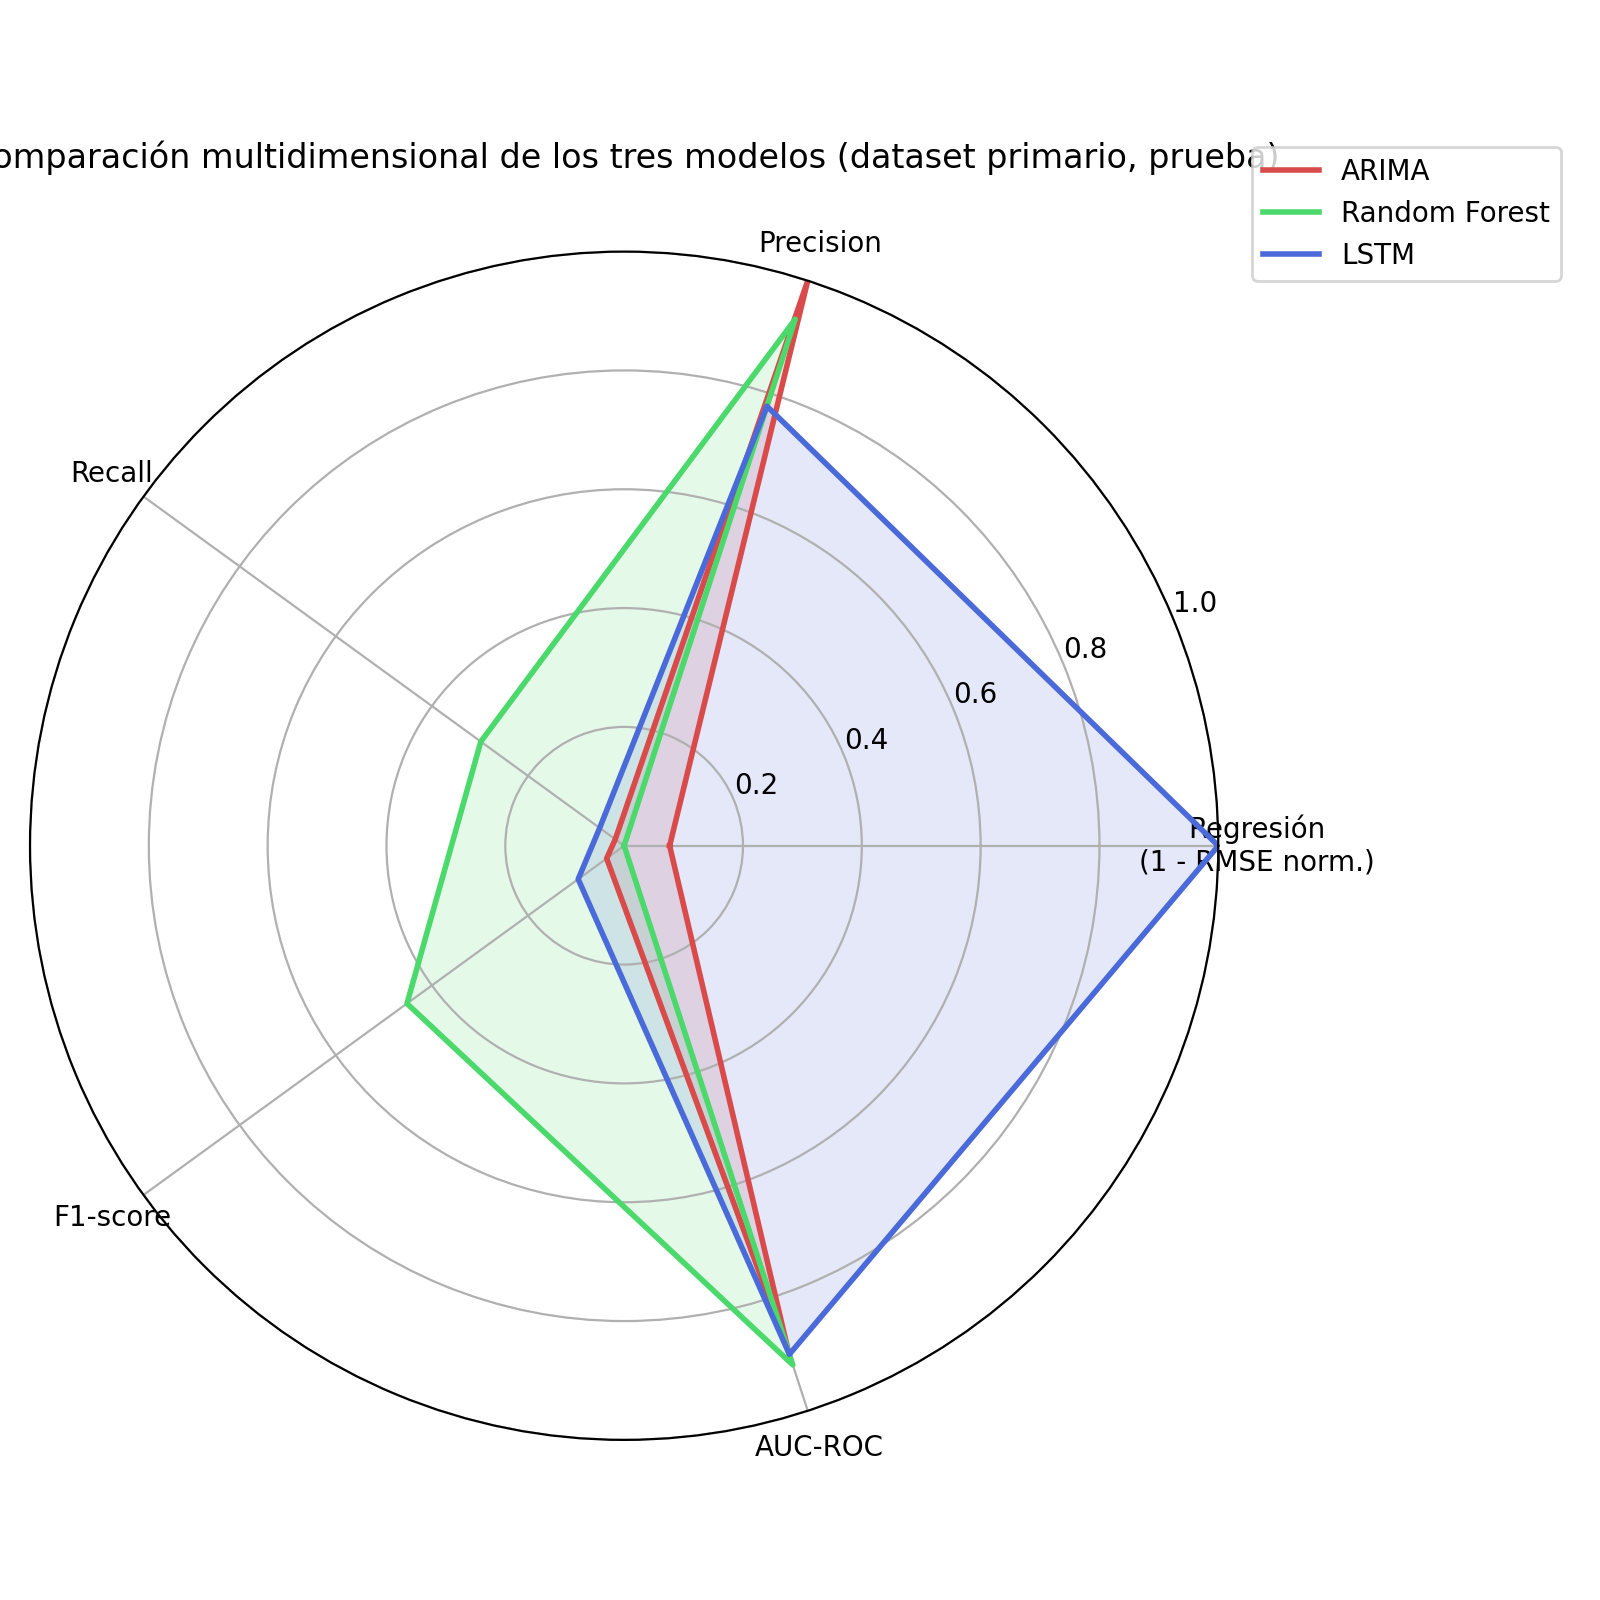
\includegraphics[width=0.7\textwidth]{radar_comparativo_modelos.png}
    \caption{Comparación multidimensional (\textit{dataset} primario, conjunto de prueba). Se constata la hiper-especialización de LSTM (regresión) frente a la robustez equilibrada de \textit{Random Forest} (\textit{F1-score}).}
    \label{fig:radar_comparativo}
\end{figure}

El análisis topológico del gráfico de radar revela tres estrategias algorítmicas divergentes:
\begin{itemize}
    \item \textbf{LSTM, polígono azul:} Su área se proyecta agresivamente hacia el eje de Regresión (dominancia absoluta en predicción basal) y exhibe un AUC-ROC sobresaliente. Sin embargo, sufre una severa contracción centrípeta en los ejes de \textit{Recall} y \textit{F1-score}, delatando su inoperancia práctica como sistema de alertamiento preventivo autónomo.
    \item \textbf{\textit{Random Forest}, polígono verde:} Presenta la geometría más equilibrada. Aunque cede el monopolio de la regresión continua frente a la red neuronal, compensa esta carencia con expansiones sólidas hacia los ejes de \textit{Recall} y Precisión, logrando la métrica armónica (\textit{F1-score} = 0.4518) más alta del experimento. Es el único modelo con viabilidad operativa dual.
    \item \textbf{ARIMA, polígono rojo:} Su perfil carece de área útil, colapsando hacia el centro en casi todas las dimensiones operativas, con la notable excepción de un pico engañoso en el eje de Precisión. Como se demostró previamente, esta aparente perfección es un artefacto matemático derivado de su extrema pasividad (predecir crisis en tan raras ocasiones que, por azar, no detonó falsas alarmas).
\end{itemize}

Para decodificar este espejismo estadístico con mayor granularidad, la Figura \ref{fig:barras_clasificacion} desagrega la comparativa en sus cinco métricas de clasificación individuales.

\begin{figure}[H]
    \centering
    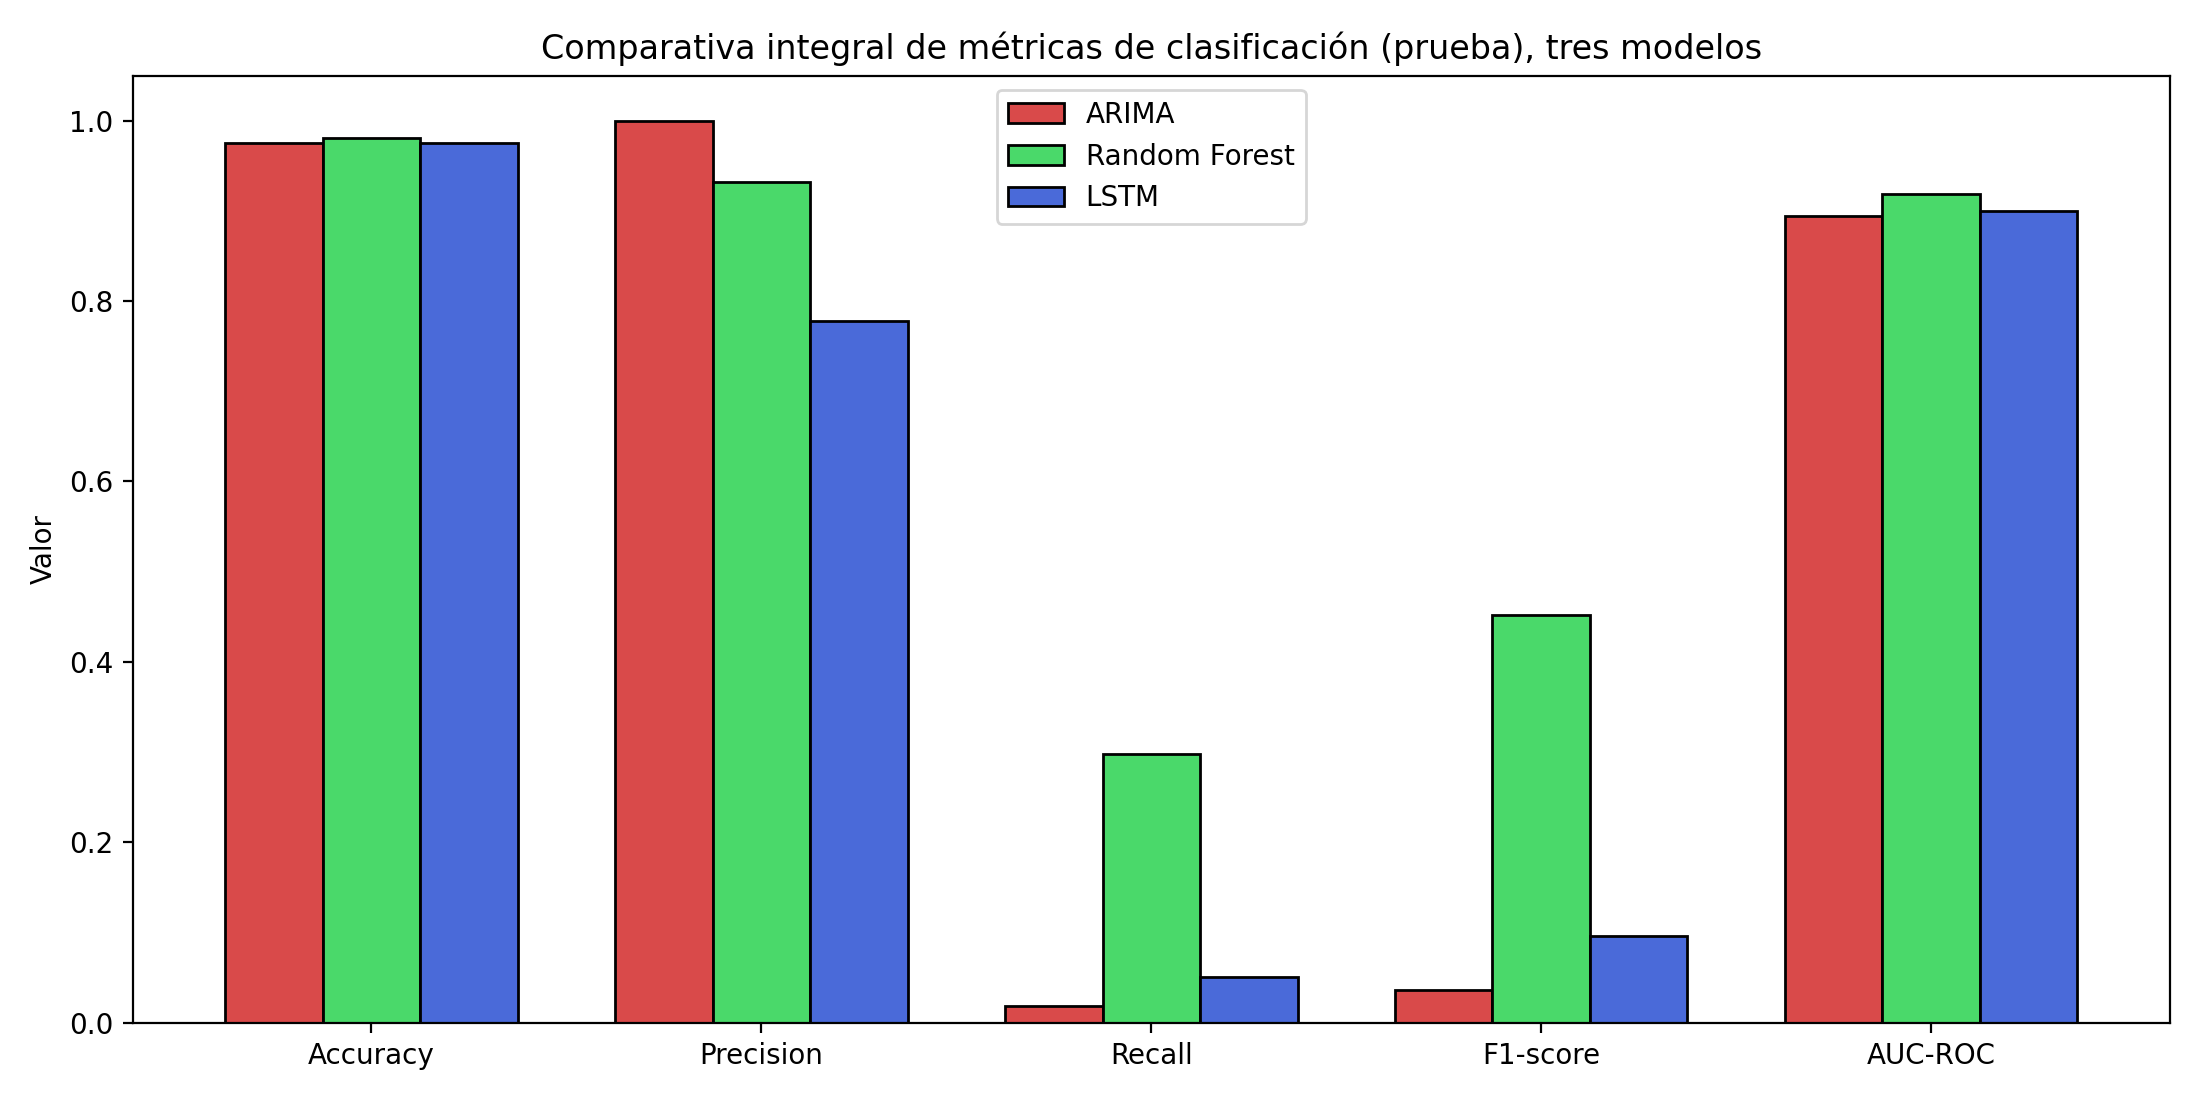
\includegraphics[width=\textwidth]{barras_clasificacion_tres_modelos.png}
    \caption{Comparativa integral de métricas de clasificación. Se evidencia el efecto engañoso de la Exactitud frente al \textit{Recall} y el \textit{F1-score} en escenarios de desbalance extremo.}
    \label{fig:barras_clasificacion}
\end{figure}

Esta descomposición de barras resulta metodológicamente reveladora y constituye una aportación crítica de esta investigación. Se observa que la Exactitud (\textit{Accuracy}) ---la métrica más intuitiva y frecuentemente sobrestimada en la literatura de redes--- resulta estadísticamente idéntica para los tres modelos (rondando el 0.98). No obstante, sus capacidades reales para detectar anomalías varían en órdenes de magnitud (evidenciado por la drástica caída en las barras de \textit{Recall} y \textit{F1-score} de ARIMA y LSTM frente a \textit{Random Forest}).

Este contraste extremo valida empíricamente la advertencia metodológica formulada en el Capítulo 4 (Sección \ref{sec:evaluacion}): en ecosistemas de red caracterizados por un desbalance de clases masivo (donde la congestión crítica representa apenas el 2.6\,\% del tiempo de operación, Sección \ref{sec:obtencion_exploracion}), la Exactitud es una métrica analíticamente inútil. Un algoritmo "tonto" que prediga letargo perpetuo obtendrá un 97.4\,\% de Exactitud sin haber detectado una sola crisis. Por consiguiente, la validación de sistemas predictivos para infraestructura crítica debe fundamentarse estrictamente en la triada de Precisión, \textit{Recall} y \textit{F1-score}.


\subsection*{Generalización entre escalas de red: una limitación transversal}

La última fila de la Tabla \ref{tab:tabla_maestra} documenta un segundo hallazgo analítico de gran relevancia: de los tres modelos, únicamente ARIMA pudo someterse a la validación exploratoria de generalización frente a MAWI bajo la granularidad oficial de 1 minuto. Su desempeño en dicho contexto (RMSE=0.3233) representa, por un margen amplio, el peor resultado de regresión obtenido en toda esta investigación ---incluso peor que su propio desempeño sobre el \textit{dataset} primario (RMSE=0.0459) o sobre el 
\textit{dataset} piloto (RMSE=0.0282)---. \textit{Random Forest} y LSTM, por su parte, no pudieron evaluarse en absoluto en este contexto debido a una incompatibilidad estructural entre sus parámetros de ventana oficiales ($w=30$ minutos) y la duración total de cada traza individual de MAWI (15 minutos continuos, documentado en las Secciones \ref{sec:resultados_rf} y \ref{sec:resultados_lstm}).

Este doble hallazgo ---el fracaso categórico de ARIMA al intentar generalizar fuera de su rango y la imposibilidad matemática de siquiera intentarlo con las topologías de \textit{Machine Learning}--- apunta a una conclusión robusta que trasciende a cualquier algoritmo individual: los tres modelos de esta tesis fueron optimizados, por diseño, para operar dentro de las características específicas de la red privada PYME bajo estudio (su escala de tráfico de bajo perfil, su granularidad de muestreo, sus rezagos temporales). 
Por consiguiente, ninguna evidencia recabada en este trabajo respalda la extrapolación directa de dichos modelos, sin reentrenamiento profundo o reajuste de ingeniería de características, hacia infraestructuras troncales de naturaleza o escala sustancialmente distinta.

\subsection*{Reconciliación con la brecha metodológica identificada en el Estado del Arte}

Resulta pertinente cerrar esta comparativa empírica retomando la brecha metodológica formulada en la síntesis del Estado del Arte (Sección \ref{sec:estado_brecha}): la ausencia, en la literatura mundial revisada, de una comparación simultánea entre los tres paradigmas de modelado bajo condiciones experimentales idénticas y controladas. 

Esta tesis cubre dicha brecha de manera directa, y el resultado de haberlo hecho es, en sí mismo, un aporte sustantivo a la disciplina. La literatura revisada tendía a presentar comparaciones aisladas o paradigmáticamente cerradas ---como el estudio de Sneha et al. \cite{sneha2020} entre variantes limitadas de \textit{Machine Learning} clásico, o el de Santos et al. \cite{santos2022} acotado exclusivamente a la batalla recurrente entre LSTM y GRU---, ninguna de las cuales podría, por diseño, haber revelado el patrón de 
especialización funcional por tarea que ha sido documentado en esta sección. 

Al someter a la estadística clásica (ARIMA), al ensamble no lineal (\textit{Random Forest}) y al \textit{Deep Learning} (LSTM) a un diseño experimental estricto y unificado ---alimentándolos con el mismo tensor de datos, el mismo umbral de decisión operativa y las mismas métricas de castigo cruzado---, este trabajo aporta evidencia concluyente de que la búsqueda del "mejor" modelo para un sistema predictivo de redes no puede resolverse en el vacío. La elección de la arquitectura adecuada depende críticamente de un factor 
operativo: si la prioridad del administrador del sistema es la precisión sostenida de la estimación continua (terreno dominado por el LSTM), o la sensibilidad preventiva e inmediata ante el evento discreto y anómalo (terreno dominado por el \textit{Random Forest}). Este es un matiz analítico que resulta frecuentemente omitido o subestimado en la bibliografía actual.

Los hallazgos aquí sintetizados ---el \textit{trade-off} central entre regresión y clasificación, la falacia matemática de la Exactitud en ambientes desbalanceados, y la dura frontera de la generalización entre escalas de red--- se retoman e interpretan en su conjunto, a la luz del problema de investigación original planteado en el Capítulo 1, en la discusión final de la Sección 6.5.
\newpage

\section{Discusión}
\label{sec:discusion}

Los hallazgos presentados a lo largo de este capítulo ---individualmente en las Secciones \ref{sec:resultados_arima} a \ref{sec:resultados_lstm}, y de manera integrada en la Sección \ref{sec:comparativa_modelos}--- permiten ahora regresar a las preguntas que dieron origen a esta investigación. Esta sección interpreta dichos hallazgos a la luz del problema de investigación planteado en el Capítulo 1, los contrasta contra el marco teórico desarrollado en el Capítulo 2 y la evidencia de la literatura revisada en el Capítulo 3, 
y discute las limitaciones que se desprenden del diseño experimental adoptado, sentando las bases para las conclusiones formales del Capítulo 7.

\subsection*{Retorno al problema de investigación}

El Capítulo 1 formuló el problema de esta tesis como una pregunta concreta: \textit{¿Es posible, a partir del análisis de datos históricos de operación de una red, construir un modelo capaz de predecir con suficiente antelación que un enlace alcanzará un estado de congestión, de tal forma que dicha predicción resulte útil para la toma de decisiones antes de que la degradación del servicio se materialice?} 

La evidencia recabada en este capítulo permite responder a esta pregunta de manera matizada, no binaria. Sí es posible construir modelos que predicen con notable precisión el comportamiento continuo del tráfico de la infraestructura estudiada ---\textit{Deep Learning} (LSTM) lo demostró con un RMSE de 0.0010 sobre datos reales nunca vistos durante el entrenamiento (Sección \ref{sec:resultados_lstm})---. Sin embargo, la utilidad práctica de dicha predicción para la toma de decisiones depende de la capacidad del sistema 
para señalar el cruce de un umbral crítico de acción (la formulación de clasificación establecida en la metodología). En esa dimensión específica, ningún modelo evaluado alcanzó un desempeño que pueda calificarse de infalible: el \textit{Recall} máximo observado, 29.82\,\% con \textit{Random Forest} (Tabla \ref{tab:tabla_maestra}), implica que una porción significativa de los eventos anómalos habrían pasado inadvertidos.

Esta disociación entre "predecir bien el valor general" y "detectar bien el evento crítico" no es un fracaso del diseño experimental, sino la aportación empírica central de esta tesis. Como se argumentó en la Sección \ref{sec:evaluacion}, la razón por la cual esta investigación priorizó el \textit{Recall} ---por encima de la Exactitud aislada--- es precisamente la asimetría de costos entre un falso negativo (una congestión no anticipada, que reproduce exactamente la limitación reactiva descrita en el Planteamiento del Problema) 
y un falso positivo (una alerta preventiva injustificada). Bajo ese criterio, el hallazgo de esta tesis no es que los modelos "fallen", sino que revela con precisión cuantitativa \textit{cuánto} camino queda por recorrer antes de que un sistema de este tipo pueda desplegarse con confianza operativa autónoma ---una distinción que posee mayor rigor científico que reportar una única métrica optimista y agregada.

\subsection*{Un hallazgo no anticipado: la disociación entre regresión y clasificación}

Ninguno de los trabajos de \textit{Machine Learning} clásico o \textit{Deep Learning} revisados en el Estado del Arte documentó explícitamente esta disociación. Como se señaló en la síntesis de dicho capítulo (Sección \ref{sec:estado_brecha}), la mayoría de la literatura mundial evalúa sus modelos mediante métricas de error continuo (RMSE, MAE, MAPE) sin traducir dicho desempeño a un criterio de clasificación accionable. La Tabla \ref{tab:reconciliacion_hallazgo} sintetiza cómo este hallazgo se conecta con la evidencia teórica 
y empírica de los capítulos anteriores.

\begin{table}[H]
    \centering
    \small
    \begin{tabular}{|p{3.3cm}|p{5.2cm}|p{5.2cm}|}
        \hline
        \textbf{Fuente} & \textbf{Lo que anticipaba} & \textbf{Lo que esta tesis encontró} \\
        \hline
        Sección \ref{sec:modelos_justificacion} (justificación de modelos) & LSTM, al capturar dependencias de largo plazo, tendría ventaja general sobre ARIMA y \textit{Random Forest}. & LSTM domina en regresión, pero queda relegado al segundo lugar en clasificación. \\
        \hline
        Oliveira et al. \cite{oliveira2016} & Mayor complejidad arquitectónica no garantiza mejor desempeño. & Confirmado y extendido: la complejidad ni siquiera garantiza mejor desempeño \textit{dentro del mismo modelo} al cambiar de tarea (regresión a clasificación). \\
        \hline
        Sección \ref{sec:evaluacion} (advertencia sobre Exactitud) & Bajo desbalance de clases, la Exactitud (\textit{Accuracy}) oculta el desempeño real. & Confirmado empíricamente: Exactitud casi idéntica (0.975--0.981) entre modelos cuyo \textit{Recall} difiere en un factor de 16 (Figura \ref{fig:barras_clasificacion}). \\
        \hline
    \end{tabular}
    \caption{Reconciliación del hallazgo central de esta tesis con el marco teórico y metodológico de capítulos anteriores.}
    \label{tab:reconciliacion_hallazgo}
\end{table}

\subsection*{La congestión como fenómeno raro: coherencia con la teoría de colas}

El hallazgo, ya documentado en la Sección \ref{sec:obtencion_exploracion}, de que la utilización real de la red privada bajo estudio nunca superó el 1.44\,\% durante los 21 días de recolección, podría interpretarse erróneamente como una falla de la investigación. Por el contrario, este resultado es plenamente coherente con el fundamento teórico desarrollado en la Sección \ref{sec:congestion}: la teoría de colas de Kleinrock \cite{kleinrock1976} predice que el tiempo de espera y la probabilidad de pérdida crecen de forma no lineal 
---proporcional a $\frac{1}{1-\rho}$--- únicamente en la vecindad de la saturación ($\rho \to 1$). Mientras la utilización se mantenga moderada, el sistema opera sin manifestar los síntomas de congestión. La ausencia de RTT elevado o pérdida de paquetes en los 21 días reales no contradice la física de redes: la confirma. 

Es, de hecho, la misma teoría de colas la que justificó la necesidad imperativa de inyectar eventos de congestión sintéticos: sin una intervención deliberada, ningún modelo matemático podría jamás aprender a predecir un fenómeno no lineal que nunca ha observado. Esta rareza estadística del evento es la razón de ser de esta investigación. El desbalance de clases documentado (2.6\,\% de casos positivos) no es un defecto del \textit{dataset}, sino un reflejo termodinámico fiel de la naturaleza del fenómeno estudiado en una red operando 
en condiciones normales.

\subsection*{Implicaciones operativas: protocolo de mitigación propuesto}

Más allá del análisis topológico, el problema de investigación y los objetivos planteados al inicio de este proyecto exigen que el sistema predictivo resulte útil para la administración operativa. Considerando que \textit{Random Forest} y LSTM demostraron un Tiempo de Anticipación Efectivo ($TAE$) promedio de 2.8 y 3.9 minutos respectivamente, este margen temporal ---impensable en esquemas reactivos tradicionales--- abre una ventana crítica para la intervención automatizada o manual.

Para capitalizar esta anticipación algorítmica, se propone el siguiente protocolo de mitigación estructurado. Una vez que el sistema predictivo detone una alerta de congestión inminente ($U(t+h) \geq 0.80$), el administrador de red (o un \textit{script} orquestador integrado al \textit{router} MikroTik) dispondrá de aproximadamente 3 minutos para ejecutar acciones escalonadas:
\begin{enumerate}
    \item \textbf{Activación de QoS dinámico (Minuto 1):} Aplicar políticas de Calidad de Servicio mediante \textit{Simple Queues} o \textit{Queue Trees} en RouterOS para priorizar el tráfico crítico (e.g., telefonía IP, bases de datos) y limitar el ancho de banda de servicios de fondo (e.g., sincronización de Nextcloud).
    \item \textbf{Enrutamiento de respaldo (Minuto 2):} Si la alerta persiste y la magnitud proyectada por LSTM apunta a la saturación total, desviar el tráfico no esencial hacia una interfaz WAN secundaria (esquema de \textit{Failover} preventivo).
    \item \textbf{Degradación controlada (Minuto 3):} Reducir temporalmente el \textit{bitrate} de las cámaras de videovigilancia en la red local antes de que los \textit{buffers} de transmisión se saturen y comience la pérdida de paquetes indiscriminada.
\end{enumerate}
Este protocolo demuestra la viabilidad de transformar un dictamen tensorial en una herramienta de gestión estratégica de redes.

\subsection*{Una implicación de diseño emergente: hacia un sistema híbrido}

El hallazgo de que ningún modelo individual domina ambas tareas (Sección \ref{sec:comparativa_modelos}, Figura \ref{fig:scatter_tradeoff}) sugiere una vía de solución innovadora: un esquema de \textbf{alertamiento híbrido}. En esta arquitectura, \textit{Random Forest} ---el modelo de mayor \textit{Recall}--- operaría como el mecanismo primario de detonación rápida de alertas, mientras que LSTM ---el modelo de menor error continuo--- complementaría dicha alerta calculando con altísima precisión la magnitud y trayectoria esperada de 
la saturación. La Figura \ref{fig:esquema_hibrido} ilustra conceptualmente esta arquitectura.

\begin{figure}[H]
    \centering
    \begin{tikzpicture}[
        every node/.style={font=\sffamily\footnotesize},
        box/.style={rectangle, draw=black!70, thick, rounded corners=3pt, align=center, minimum height=1.1cm, minimum width=3.2cm, fill=gray!5},
        arrow/.style={-{Latex[length=2.5mm]}, thick}
    ]
    \node[box] (entrada) {Métricas de red\\ en tiempo real};
    \node[box, below left=1.2cm and -0.3cm of entrada, fill=black!10] (rf) {\textit{Random Forest}\\ \footnotesize (\textit{Recall}=0.298)};
    \node[box, below right=1.2cm and -0.3cm of entrada, fill=black!10] (lstm) {LSTM\\ \footnotesize (RMSE=0.0010)};
    \node[box, below=2.6cm of entrada, fill=black!20, minimum width=5cm] (alerta) {¿\textit{Random Forest} detecta\\ posible congestión?};
    \node[box, below=1.1cm of alerta, fill=black!30, minimum width=5cm] (salida) {Alerta + estimación de magnitud\\ (aportada por LSTM)};

    \draw[arrow] (entrada) -- (rf);
    \draw[arrow] (entrada) -- (lstm);
    \draw[arrow] (rf) -- (alerta);
    \draw[arrow] (alerta) -- (salida);
    \draw[arrow] (lstm.south) |- (salida.east);
    \end{tikzpicture}
    \caption{Esquema conceptual de un sistema de alertamiento híbrido, combinando la sensibilidad de detección de \textit{Random Forest} con la precisión de estimación continua de LSTM.}
    \label{fig:esquema_hibrido}
\end{figure}

Esta propuesta no fue implementada empíricamente en el alcance de este trabajo, pero se retoma formalmente como línea de trabajo futuro en el Capítulo 7, dado que se desprende con naturalidad del patrón de especialización complementaria descubierto.

\subsection*{Cierre de las brechas identificadas en el Estado del Arte}

Para concluir esta discusión, la Tabla \ref{tab:cierre_brechas} retoma las tres brechas formuladas al final de la revisión de la literatura (Sección \ref{sec:estado_brecha}) y contrasta cada una contra la evidencia generada.

\begin{table}[H]
    \centering
    \small
    \begin{tabular}{|p{3cm}|p{5.5cm}|p{5.2cm}|}
        \hline
        \textbf{Brecha (Sección \ref{sec:estado_brecha})} & \textbf{Cómo se abordó} & \textbf{Evidencia generada} \\
        \hline
        Conceptual: predicción de volumen vs. congestión como evento discreto. & Se definió y aplicó una variable objetivo de clasificación explícita ($U \geq U_{th}$), evaluada de forma independiente a la regresión. & Tablas \ref{tab:recap_arima_primario_clasificacion}, \ref{tab:recap_rf_primario_clasificacion}, \ref{tab:recap_lstm_primario_clasificacion}. \\
        \hline
        Metodológica: ausencia de comparación simultánea entre paradigmas. & Los tres modelos se entrenaron y evaluaron bajo condiciones idénticas (mismos datos, mismo umbral, mismas métricas). & Tabla maestra \ref{tab:tabla_maestra}, Sección \ref{sec:comparativa_modelos}. \\
        \hline
        De validación: dependencia de una única fuente de datos. & Se adoptó un \textit{dataset} híbrido y se intentó una validación cruzada externa contra el \textit{dataset} público MAWI. & Sección \ref{sec:obtencion_exploracion} (diseño híbrido); limitación de portabilidad documentada en la Sección \ref{sec:comparativa_modelos}. \\
        \hline
    \end{tabular}
    \caption{Cierre de las brechas del Estado del Arte a la luz de los resultados del Capítulo 6.}
    \label{tab:cierre_brechas}
\end{table}

Las tres brechas fueron abordadas de manera directa; sin embargo, como revela la última fila de la Tabla \ref{tab:cierre_brechas}, la brecha de validación se cerró solo parcialmente. Este es un resultado honesto que, lejos de restar valor a este trabajo, delimita con precisión científica el punto exacto en el que una futura extensión de esta línea de investigación debería concentrar sus esfuerzos.

\subsection*{Limitaciones reconocidas}

En congruencia con el compromiso de rigor metodológico sostenido, se enumeran a continuación las limitaciones estructurales que condicionan el alcance de los hallazgos:

\begin{enumerate}
    \item \textbf{Periodo de recolección acotado.} Como se documentó en los Alcances, el periodo de recolección se ajustó a 21 días efectivos. Un periodo más extenso habría permitido observar ciclos estacionales completos y, potencialmente, episodios de congestión genuinos ---por ejemplo, ante la migración de respaldos masivos de videovigilancia o sincronización de bases de datos---.
    \item \textbf{Dependencia de datos sintéticos para clasificación.} La totalidad de la evidencia de clasificación presentada proviene de anomalías inyectadas sobre el tráfico de fondo. Si bien la literatura respalda el uso de tráfico simulado, el desempeño reportado es una aproximación razonada y no una medición directa sobre colapsos \textit{reales} de la infraestructura.
    \item \textbf{Fricción en la generalización de escalas.} Únicamente ARIMA pudo evaluarse de forma exploratoria frente a MAWI. Las arquitecturas de \textit{Machine Learning}, por incompatibilidad estructural entre los parámetros de ventana y las capturas, no pudieron someterse a esta prueba. Los hallazgos son válidos específicamente para el contexto de la infraestructura estudiada y no garantizan aplicabilidad universal instantánea.
    \item \textbf{Fuente única de telemetría primaria.} El \textit{dataset} primario proviene de un único \textit{router} operando en un entorno PYME específico. Sus patrones de tráfico de baja utilización son característicos de este despliegue particular y no necesariamente representativos del comportamiento global de otras redes corporativas.
\end{enumerate}

\chapter{Conclusiones}
\label{cap:conclusiones}

El presente trabajo de tesis se propuso, desde su planteamiento original (Sección 1.1), resolver una problemática de ingeniería fundamental: evaluar la viabilidad de construir un sistema predictivo capaz de anticipar la congestión en una red de datos, habilitando con ello la transición de una administración de infraestructura empírica y reactiva hacia una gestión algorítmica y preventiva. 

A lo largo de los capítulos precedentes, este desafío fue delimitado conceptualmente mediante la formalización operativa de la congestión (Sección \ref{sec:congestion}) y la identificación de brechas críticas en la literatura (Sección \ref{sec:estado_brecha}). Posteriormente, fue abordado mediante un diseño metodológico riguroso que combinó la recolección de telemetría real con la inyección calibrada de anomalías sintéticas para subsanar el desbalance de clases (Sección \ref{sec:obtencion_exploracion}). Finalmente, el problema fue sometido a escrutinio empírico a través del diseño, entrenamiento y evaluación comparativa exhaustiva de tres paradigmas de modelado: la estadística clásica autorregresiva (ARIMA), los ensambles de árboles de decisión (\textit{Random Forest}) y las redes neuronales recurrentes de memoria a corto y largo plazo (LSTM) (Capítulos 5 y 6).

Corresponde a este capítulo final desempeñar una función de síntesis analítica: no generar nueva evidencia empírica, sino articular, con rigor y honestidad intelectual, las conclusiones definitivas que dicha evidencia permite sostener. Para lograr este cometido, el capítulo se estructura en dos ejes fundamentales. 

En primera instancia, la Sección 7.1 detalla las contribuciones concretas que esta investigación aporta tanto a la comunidad académica como a la práctica profesional de la ingeniería de redes, diferenciando sistemáticamente entre hallazgos metodológicos, empíricos y operativos. Finalmente, la Sección 7.2 expone con total transparencia las limitaciones inherentes al diseño experimental implementado ---muchas de ellas anticipadas en los alcances originales de la tesis (Sección 1.4) y confirmadas algorítmicamente en la fase de generalización---. A partir de estas restricciones, se formulan líneas directas de trabajo futuro, garantizando que los límites topológicos de este estudio no representen un cierre definitivo, sino el cimiento legítimo para la evolución continua de los sistemas predictivos de red.

\section{Contribuciones}
\label{sec:contribuciones}

Más allá de la demostración de los paradigmas predictivos, esta investigación aporta valor empírico, metodológico y operativo ---atribuible directamente a las decisiones de diseño del autor--- a la comunidad académica y a la práctica profesional de la administración de redes. Dichas contribuciones se estructuran en las siguientes tres vertientes:

\subsection*{Contribuciones metodológicas}

\begin{itemize}
    \item \textbf{Estrategia reproducible de aumento de datos sin contaminación (\textit{Data Leakage}):} Ante la infrecuencia empírica de la congestión severa, se diseñó e implementó un esquema de inyección sintética calibrada estadísticamente. Esta inyección incluye aserciones matemáticas en tiempo de ejecución que garantizan el aislamiento absoluto entre las particiones de entrenamiento y evaluación, subsanando una vulnerabilidad metodológica recurrente en la literatura del campo.
    \item \textbf{Fundamentación de la métrica objetivo en la Teoría de Colas:} A diferencia de enfoques predictivos agnósticos al contexto, la variable objetivo de congestión se operacionalizó basándose en el comportamiento asintótico no lineal del retraso postulado por Kleinrock. Esta definición unificó los criterios de evaluación y guio matemáticamente la inyección sintética, cerrando el ciclo entre el marco teórico y la experimentación empírica.
\end{itemize}

\subsection*{Contribuciones empíricas}

\begin{itemize}
    \item \textbf{Descubrimiento del \textit{Trade-off} predictivo entre arquitecturas:} Al someter los tres paradigmas algorítmicos (Estadístico, Ensambles y \textit{Deep Learning}) a condiciones experimentales idénticas, se demostró empíricamente la disociación matemática entre regresión continua y clasificación binaria. Se evidenció que la LSTM dominó la precisión del flujo basal, mientras que \textit{Random Forest} dominó la sensibilidad de alertamiento. Este hallazgo refuta la superioridad infalible frecuentemente atribuida a las redes neuronales en la literatura general.
    \item \textbf{Estudio de caso en topologías asimétricas de pequeña escala:} Se documenta de forma transparente el comportamiento de una red PYME real (telemetría, videovigilancia y sincronización en la nube), caracterizada por un régimen de letargo extremo (utilización $\leq$ 1.44\,\%). Este esfuerzo enriquece un campo académico históricamente sesgado hacia infraestructuras troncales masivas o entornos de laboratorio hiper-controlados.
    \item \textbf{Identificación de límites de generalización en repositorios públicos:} La evaluación cruzada reveló que arquitecturas como MAWI (cuyas trazas están limitadas a 15 minutos continuos) resultan estructuralmente incompatibles para validar modelos de \textit{Machine Learning} que dependen de ventanas temporales ($w$) extensas, estableciendo un precedente crítico para futuras investigaciones sobre dichos repositorios.
\end{itemize}

\subsection*{Contribuciones de ingeniería de \textit{software}}

\begin{itemize}
    \item \textbf{Decodificador \textit{libpcap} de bajo perfil de memoria (\textit{Streaming}):} Se desarrolló un \textit{script} original en Python capaz de interpretar la estructura binaria de paquetes a nivel de \textit{byte} sin saturar la memoria RAM. Esta herramienta viabiliza el procesamiento de decenas de millones de paquetes en estaciones de trabajo convencionales, democratizando el análisis de grandes volúmenes de telemetría de red.
    \item \textbf{Instrumentación de telemetría asíncrona mediante RouterOS:} Ante la imposibilidad técnica de emplear SNMP por restricciones de infraestructura (ausencia de IP pública), se instrumentó una solución \textit{ad hoc} explotando los \textit{scripts} nativos y el \textit{Scheduler} del equipo MikroTik. Este desarrollo aporta una plantilla práctica invaluable para el monitoreo de redes remotas sujetas a políticas de seguridad estrictas.
\end{itemize}

\section{Limitaciones del estudio}
\label{sec:limitaciones}

La rigurosidad de toda investigación en ingeniería exige el reconocimiento explícito de sus fronteras metodológicas y empíricas. Las limitaciones documentadas en esta sección no invalidan los hallazgos expuestos en los capítulos precedentes, sino que delimitan con precisión su contexto de aplicabilidad, garantizando la honestidad intelectual del estudio y estableciendo el punto de partida exacto para la continuidad del desarrollo tecnológico.

La Tabla \ref{tab:limitaciones_resumen} sintetiza el escrutinio de estas restricciones, categorizándolas según su origen estructural: (a) limitaciones de alcance declaradas por diseño; (b) restricciones logísticas y computacionales derivadas del entorno de ejecución; y (c) limitantes topológicas y algorítmicas descubiertas empíricamente durante la fase de evaluación. Para cada restricción se identifica su efecto directo sobre las conclusiones y se vincula con la línea de trabajo futuro destinada a solventarla.

\begin{table}[H]
    \centering
    \small
    \begin{tabular}{|p{4.1cm}|p{1.7cm}|p{4.6cm}|p{2.6cm}|}
        \hline
        \textbf{Limitación} & \textbf{Origen} & \textbf{Efecto sobre las conclusiones} & \textbf{Continuación} \\
        \hline
        Ausencia de interfaz gráfica, empaquetado de \textit{software} u operación en producción. & (a) & Ninguno sobre la viabilidad predictiva; restringe la utilidad operativa inmediata para administradores. & Trabajo futuro 1 \\
        \hline
        Carencia de alertamiento en tiempo real y evaluación del Tiempo de Antelación (TAE) operativo. & (a)/(c) & La utilidad para la toma de decisiones se argumenta a nivel analítico, sin demostración en flujo continuo. & Trabajo futuro 2 \\
        \hline
        Recolección acotada a 21 días (82.9\,\% de cobertura) frente a los 60 días proyectados. & (b) & Reducción de ciclos estacionales evaluables; ausencia empírica de eventos de congestión masiva nativa. & Trabajo futuro 3 \\
        \hline
        Evaluación sobre una topología única con régimen de letargo extremo (utilización máxima 1.44\,\%). & (b)/(c) & Impide la extrapolación directa de los pesos y umbrales algorítmicos hacia infraestructuras corporativas densas. & Trabajo futuro 3 \\
        \hline
        Desempeño de clasificación evaluado exclusivamente sobre inyecciones sintéticas aisladas. & (c) & El \textit{Recall} documentado representa una cota estadística de sensibilidad, no una métrica operativa sobre crisis reales. & Trabajo futuro 4 \\
        \hline
        Diseño de características (\textit{features}) restringido a la utilización del canal. & (c) & Omite el contraste empírico de vectores latentes como pérdida de paquetes, RTT y periodicidad de calendario. & Trabajo futuro 5 \\
        \hline
        Arquitecturas SVR y GRU descartadas; búsqueda de hiperparámetros acotada y ejecución exclusiva en CPU. & (a)/(b) & Conclusiones circunscritas estrictamente a los tres algoritmos base bajo configuraciones estructurales conservadoras. & Trabajo futuro 5 \\
        \hline
        Etiqueta de estado y umbral de congestión ($U_{th}$) fijados analíticamente, sin contraste dinámico. & (c) & Simplifica la detección, ignorando la adaptabilidad requerida para líneas base de tráfico mutables. & Trabajo futuro 4 \\
        \hline
        Ejecución única sin cálculo de intervalos de confianza; evaluación de MAWI reducida a 6 tensores. & (b)/(c) & Las brechas de magnitud superior son categóricas, pero las variaciones porcentuales finas carecen de significancia estadística plena. & Trabajo futuro 6 \\
        \hline
        Validación de generalización (MAWI) ejecutable de manera exclusiva para el modelo ARIMA. & (c) & Ausencia total de evidencia sobre la portabilidad matemática de \textit{Random Forest} y LSTM ante restricciones de ventana temporal. & Trabajo futuro 6 \\
        \hline
    \end{tabular}
    \caption{Síntesis de limitaciones operativas, logísticas y empíricas del estudio, su impacto en las afirmaciones de la tesis y su directriz metodológica de resolución.}
    \label{tab:limitaciones_resumen}
\end{table}

\subsection*{Alcance del prototipo y métricas operativas}

El alcance operativo del prototipo se circunscribió estrictamente a la demostración matemática de viabilidad predictiva en un entorno fuera de línea (\textit{offline}), prescindiendo del desarrollo de interfaces gráficas, ingestión continua de telemetría o arquitecturas de reentrenamiento autónomo (\textit{concept drift}). Esta decisión priorizó el rigor del diseño experimental y la evaluación algorítmica sobre el empaquetado de un producto comercial. 

Como consecuencia directa de este enfoque y de la escasez de anomalías reales, los mecanismos automatizados de alertamiento y la métrica de Tiempo de Anticipación Efectivo ($TAE$) no fueron evaluados operativamente. Dado que la congestión sostenida en el \textit{dataset} primario provino de inyecciones sintéticas con rampas de ascenso predefinidas, el cálculo del $TAE$ habría medido la morfología estática del generador algorítmico y no la agudeza orgánica del modelo, careciendo además de significancia estadística ante el reducido volumen de detecciones efectivas en la tarea de clasificación.
\subsection*{Restricciones topológicas y dimensionalidad de variables}

La recolección de telemetría se acotó a 21 días efectivos sobre una única infraestructura PYME, caracterizada por un régimen de tráfico crónicamente ocioso (utilización $\leq$ 1.44\,\%). Esta limitación topológica impidió el modelado sobre anomalías orgánicas, por lo que los pesos sinápticos resultantes están fuertemente condicionados a este ecosistema particular y exigen un proceso de \textit{fine-tuning} previo a cualquier extrapolación.

Asimismo, el espacio de características (\textit{features}) se contrajo de forma exclusiva al factor de utilización y sus rezagos. El RTT y la pérdida de paquetes reales carecían de entropía operativa (con asintonía a cero); intentar inyectarlos de forma sintética habría provocado una fuga de datos (\textit{target leakage}), al derivarse determinísticamente de la misma ecuación de congestión (Ecuación \ref{eq:congestion_instanciada}). Las restricciones computacionales también limitaron la evaluación a tres arquitecturas representativas (excluyendo alternativas como SVR y GRU), evaluadas en un único horizonte predictivo ($h=5$ minutos) y procesadas íntegramente en CPU, acotando la validez estricta de los resultados a dichas configuraciones.
\subsection*{Sesgos en la inyección sintética y evaluación}

La validación de la tarea de clasificación descansa sobre datos sintéticos, lo que conlleva tres sesgos estadísticos explícitos: (1) la ausencia de inercia estocástica temporal en el ruido de fondo (producto del remuestreo independiente); (2) el uso de perfiles de congestión geométricamente estilizados (trapezoidales) que podrían inducir al modelo a detectar patrones matemáticos artificiales en lugar de saturaciones orgánicas; y (3) la ejecución de la evaluación sobre la misma distribución generativa del entrenamiento. Estos sesgos garantizan una comparación transversal justa entre modelos, pero prohíben interpretar numéricamente el \textit{Recall} documentado como una garantía de rendimiento infalible en un entorno de producción inexplorado.

Por su parte, el protocolo de evaluación careció de repeticiones masivas estocásticas (estilo Montecarlo) para el cálculo de intervalos de confianza, y la validación de generalización contra MAWI se restringió a 6 observaciones exclusivas para ARIMA. Esto ocurrió debido a que las ventanas estructurales de los modelos de \textit{Machine Learning} ($w=30$ minutos) resultaron algorítmicamente incompatibles con las capturas fragmentadas de 15 minutos del repositorio japonés, impidiendo evaluar empíricamente su portabilidad inter-dominio.

\subsection*{Alcance absoluto de las conclusiones}

Como epílogo de este ejercicio crítico, la Tabla \ref{tab:alcance_conclusiones} traza una frontera diáfana entre las afirmaciones que cuentan con el respaldo irrestricto de la evidencia recabada y aquellas presunciones que el rigor metodológico desautoriza categóricamente.

\begin{table}[H]
    \centering
    \small
    \begin{tabular}{|p{6.4cm}|p{6.4cm}|}
        \hline
        \textbf{Afirmaciones sostenidas por la evidencia} & \textbf{Presunciones no sostenidas por la evidencia} \\
        \hline
        LSTM predice con el menor error probabilístico el flujo de tráfico orgánico de la red privada estudiada (Sección \ref{sec:resultados_lstm}). & Que cualquiera de estos modelos logre detectar una crisis de congestión puramente humana con la misma sensibilidad reportada sobre los datos sintéticos. \\
        \hline
        Bajo las rigurosas condiciones evaluadas, ningún modelo algorítmico logra dominar de manera simultánea las tareas de regresión continua y clasificación discreta (Sección \ref{sec:comparativa_modelos}). & Que el orden jerárquico de eficacia (LSTM $>$ \textit{Random Forest} $>$ ARIMA en regresión) se mantenga inmutable ante nuevas \textit{features} o arquitecturas. \\
        \hline
        En escenarios de red asimétricos (masivo desbalance de clases), la Exactitud (\textit{Accuracy}) resulta ser una métrica matemáticamente engañosa e insuficiente (Figura \ref{fig:barras_clasificacion}). & Que la arquitectura resultante esté lista para un despliegue operativo en producción sin requerir fases de prueba beta y evaluación de latencia. \\
        \hline
        Un algoritmo ARIMA calibrado en la dinámica ociosa de una red menor fracasa estrepitosamente al intentar generalizar sobre un enlace troncal académico de uso intenso (Sección \ref{sec:resultados_arima}). & Que los algoritmos de \textit{Machine Learning} sean infalibles a la hora de generalizar, dado que la disparidad en las longitudes de captura impidió comprobarlo. \\
        \hline
    \end{tabular}
    \caption{Delimitación rigurosa del alcance científico de las conclusiones dictaminadas en esta investigación.}
    \label{tab:alcance_conclusiones}
\end{table}

La exposición de estas limitaciones metodológicas no invalida el peso científico del dictamen central de la investigación: el diseño experimental implementado logró aislar el impacto de estas variables condicionantes, garantizando que la comparativa transversal definitiva entre los tres modelos matemáticos se mantuviera inquebrantablemente justa, equitativa y controlada.

\section{Trabajo futuro}
\label{sec:trabajo_futuro}

Las limitaciones y descubrimientos empíricos documentados en esta tesis no representan un punto final, sino que trazan una hoja de ruta estructurada para la evolución de los sistemas predictivos de red. Se proponen las siguientes seis líneas estratégicas de continuación:

\begin{enumerate}
    \item \textbf{Operacionalización y despliegue en tiempo real.} Evolucionar los \textit{scripts} algorítmicos validados \textit{offline} hacia una arquitectura de producción. Esto requiere desarrollar conductos de ingestión continua de telemetría (vía API o gRPC nativo de \textit{routers}), interfaces gráficas de usuario (\textit{dashboards}) y rutinas de reentrenamiento autónomo que mitiguen el cambio de concepto (\textit{concept drift}).
    \item \textbf{Alertamiento híbrido y evaluación operativa del $TAE$.} Instrumentar en un entorno vivo el orquestador conceptualizado en la Figura \ref{fig:esquema_hibrido}, empleando \textit{Random Forest} como percutor rápido de alarmas y LSTM como proyector de impacto continuo. Esto permitirá medir empíricamente el Tiempo de Anticipación Efectivo ($TAE$) ante crisis orgánicas y validar la integración de mitigaciones automatizadas en arquitecturas \textit{Software-Defined Networking} (SDN).
    \item \textbf{Expansión longitudinal y escalabilidad topológica.} Extender la captura de telemetría a ciclos multimensuales para internalizar patrones estacionales (e.g., respaldos masivos y mantenimientos). Paralelamente, evaluar el despliegue del sistema en infraestructuras corporativas densas, analizando cómo debe mutar la dimensionalidad de las características (\textit{features}) al transitar entre distintas escalas de red.
    \item \textbf{Validación orgánica del umbral y rediseño de la variable objetivo.} Sustituir la inyección de tráfico sintético mediante la correlación con bitácoras reales de incidentes (\textit{tickets} de soporte). Esto permitirá validar empíricamente si el umbral heurístico del 80\% ($U_{th}=0.80$) detona inflexiones comprobables en el RTT y el \textit{Jitter} a nivel de usuario, y facilitará la reprogramación del tensor para evaluar congestión sostenida en lugar del cruce probabilístico instantáneo.
    \item \textbf{Enriquecimiento dimensional y arquitecturas de frontera.} Integrar al tensor predictivo variables de Capa 4 (e.g., retransmisiones TCP) y codificaciones temporales, evaluándolas sobre una red con mayor entropía dinámica. Bajo estas nuevas condiciones, escalar la comparativa algorítmica hacia topologías SVR, GRU y Mecanismos de Atención (\textit{Transformers}), apalancando clústeres GPU para búsquedas hiperparamétricas exhaustivas.
    \item \textbf{Robustez estocástica y portabilidad inter-dominio.} Automatizar pruebas de reentrenamiento estocástico masivo (métodos Montecarlo) para establecer intervalos de confianza estadísticamente irrefutables. Asimismo, desarrollar estrategias de adaptación de dimensionalidad (\textit{padding}) que compatibilicen ventanas tensoriales amplias (e.g., $w=30$ minutos) con capturas históricas breves (e.g., 15 minutos en repositorios MAWI), destrabando la evaluación externa de algoritmos de \textit{Deep Learning}.
\end{enumerate}
El generador sintético se calibró con la distribución horaria de los 21 días reales, incluidos los periodos posteriormente empleados como validación y prueba; en consecuencia, el entrenamiento incorpora información distribucional marginal (no secuencial) de dichos periodos, y los días sintéticos de entrenamiento poseen fechas posteriores al conjunto de prueba real. Este efecto se estima moderado, pues solo se remuestrearon valores aislados por hora, sin conservar su orden temporal, pero impide afirmar una separación temporal estricta entre entrenamiento y evaluación.

\clearpage
\addcontentsline{toc}{chapter}{Referencias bibliográficas}
\bibliographystyle{IEEEtran}
\bibliography{referencias}

\appendix
\chapter{Código fuente de ejemplos críticos}

Este apéndice reproduce el código fuente de las piezas de software consideradas más relevantes para la comprensión y reproducibilidad del prototipo desarrollado en esta tesis. Se excluyen deliberadamente los scripts de configuración de entorno, corrección de errores y depuración que no aportan al entendimiento metodológico del trabajo. El repositorio completo del proyecto contiene la totalidad de los scripts empleados.

\section{Decodificador de trazas libpcap}
\label{apx:decodificador_libpcap}

El siguiente fragmento corresponde al decodificador propio empleado para extraer telemetría de las trazas de MAWI (Sección \ref{sec:preprocesamiento_desarrollo}), evitando la sobrecarga de memoria de herramientas de disección de protocolos de alto nivel. A diferencia del fragmento presentado en el Capítulo 5 (Código \ref{lst:parser_pcap}), aquí se incluye el manejo completo de las cuatro variantes del encabezado global de \textit{libpcap} (orden de bytes y precisión temporal).

\begin{lstlisting}[language=Python, caption={Decodificador completo de trazas libpcap.}, label={lst:apx_parser_pcap}]
import struct
from collections import defaultdict

def parsear_pcap(pcap_path, ventana_seg=60):
    """
    Lee un archivo .pcap directamente (formato clasico libpcap), extrayendo
    timestamp y tamano original de cada paquete SIN decodificar protocolos.
    Agrega el volumen de bytes transmitidos en ventanas temporales discretas.
    """
    acumulado = defaultdict(int)
    contador = 0

    with open(pcap_path, "rb") as f:
        # --- Encabezado global (24 bytes) ---
        cabecera_global = f.read(24)
        magic = struct.unpack("I", cabecera_global[0:4])[0]

        if magic == 0xa1b2c3d4:
            endian = "<"   # little-endian, microsegundos
            nano = False
        elif magic == 0xd4c3b2a1:
            endian = ">"   # big-endian, microsegundos
            nano = False
        elif magic == 0xa1b23c4d:
            endian = "<"   # little-endian, nanosegundos
            nano = True
        elif magic == 0x4d3cb2a1:
            endian = ">"   # big-endian, nanosegundos
            nano = True
        else:
            raise ValueError(f"Magic number no reconocido: {hex(magic)}")

        fmt_registro = endian + "IIII"  # ts_sec, ts_usec, incl_len, orig_len

        while True:
            encabezado_paquete = f.read(16)
            if len(encabezado_paquete) < 16:
                break  # fin del archivo

            ts_sec, ts_usec, incl_len, orig_len = struct.unpack(
                fmt_registro, encabezado_paquete
            )

            if nano:
                timestamp = ts_sec + (ts_usec / 1_000_000_000)
            else:
                timestamp = ts_sec + (ts_usec / 1_000_000)

            ventana = int(timestamp // ventana_seg)
            acumulado[ventana] += orig_len
            contador += 1

            f.seek(incl_len, 1)  # salta los bytes del paquete sin leerlos

    filas = [{"timestamp": v * ventana_seg, "throughput_bps": (b * 8) / ventana_seg}
             for v, b in sorted(acumulado.items())]
    return filas, contador
\end{lstlisting}
\newpage
\section{Script de recolección en RouterOS}
\label{apx:recoleccion_routeros}

El siguiente script, escrito en RouterOS Script y ejecutado periódicamente mediante el Programador de Tareas (\textit{Scheduler}), constituye el mecanismo de recolección del dataset primario (Sección \ref{sec:fuente_datos}), adoptado como alternativa funcionalmente equivalente a SNMP ante las restricciones de acceso remoto descritas en la Sección 5.1.

\begin{lstlisting}[language=bash, caption={Script de recolección de telemetría en RouterOS.}, label={lst:apx_recoleccion_routeros}]
:local wanInterface "ether1";
:local pingTarget "1.1.1.1";

:local traf [/interface monitor-traffic interface=$wanInterface once as-value];
:local rxbps ($traf->"rx-bits-per-second");
:local txbps ($traf->"tx-bits-per-second");

:local pingResult [/ping $pingTarget count=5 as-value];
:local recibidos [:len $pingResult];
:local perdida ((5 - $recibidos) * 100 / 5);

:local sumaUs 0;
:foreach r in=$pingResult do={
    :local timeStr [:tostr ($r->"time")];
    :local hh [:tonum [:pick $timeStr 0 2]];
    :local mm [:tonum [:pick $timeStr 3 5]];
    :local ss [:tonum [:pick $timeStr 6 8]];
    :local frac [:tonum [:pick $timeStr 9 15]];
    :local totalUs ((($hh*3600)+($mm*60)+$ss)*1000000 + $frac);
    :set sumaUs ($sumaUs + $totalUs);
};
:local rttUsProm 0;
:if ($recibidos > 0) do={ :set rttUsProm ($sumaUs / $recibidos) };

:local fecha [:tostr [/system clock get date]];
:local hora [:tostr [/system clock get time]];
:local linea ($fecha . "," . $hora . "," . $rxbps . "," . $txbps . "," . $rttUsProm . "," . $perdida);
:local nombreArchivo ("log_" . $fecha . ".csv");

:if ([:len [/file find name=$nombreArchivo]] = 0) do={
    /file add name=$nombreArchivo contents=("fecha,hora,rx_bps,tx_bps,rtt_us,perdida_pct\n" . $linea . "\n")
} else={
    :local actual [/file get [find name=$nombreArchivo] contents];
    /file set [find name=$nombreArchivo] contents=($actual . $linea . "\n")
}
\end{lstlisting}

Este script se programó mediante \texttt{/system scheduler add name=run-recolectar interval=1m on-event=recolectar-metrica}, ejecutándose de manera autónoma cada minuto durante todo el periodo de recolección, con respaldo local resiliente a interrupciones de la conectividad VPN (Tabla \ref{tab:huecos_recoleccion}).

\section{Pipeline de preprocesamiento}
\label{apx:pipeline_preprocesamiento}

El siguiente script implementa las etapas de limpieza, detección de sesiones, generación de variables de rezago y definición de las variables objetivo de regresión y clasificación (Sección \ref{sec:preprocesamiento_desarrollo}), aplicado de manera uniforme a los cinco conjuntos derivados del dataset primario.

\begin{lstlisting}[language=Python, caption={Pipeline de limpieza, detección de sesiones y generación de variables.}, label={lst:apx_preprocesamiento}]
import pandas as pd
import numpy as np

BANDA_NOMINAL = 1_000_000_000
U_TH = 0.80
H = 5
UMBRAL_SESION_MIN = 5
N_REZAGOS = 5
VENTANA_MEDIA_MOVIL = 30

def procesar(path_entrada, nombre_salida, es_train=False):
    df = pd.read_csv(path_entrada)
    df["timestamp"] = pd.to_datetime(df["timestamp"])
    df = df.sort_values("timestamp").reset_index(drop=True)
    df["utilizacion"] = df["rx_bps"] / BANDA_NOMINAL

    # --- Deteccion de sesiones (huecos grandes = frontera) ---
    diffs = df["timestamp"].diff().dt.total_seconds().fillna(0) / 60.0
    df["sesion_id"] = (diffs > UMBRAL_SESION_MIN).cumsum()

    # --- Limpieza por sesion: reindexar, interpolar huecos cortos ---
    sesiones_limpias = []
    for sid, grupo in df.groupby("sesion_id"):
        grupo = grupo.sort_values("timestamp")
        rango = pd.date_range(grupo["timestamp"].min(), grupo["timestamp"].max(), freq="1min")
        g_completo = pd.DataFrame({"timestamp": rango})
        g_completo = g_completo.merge(
            grupo[["timestamp", "utilizacion", "rtt_us", "perdida_pct", "es_sintetico"]],
            on="timestamp", how="left"
        )
        g_completo["utilizacion"] = g_completo["utilizacion"].interpolate(method="linear", limit=3)
        g_completo["rtt_us"] = g_completo["rtt_us"].interpolate(method="linear", limit=3)
        g_completo["perdida_pct"] = g_completo["perdida_pct"].interpolate(method="linear", limit=3)
        g_completo["es_sintetico"] = g_completo["es_sintetico"].ffill().bfill()
        g_completo["sesion_id"] = sid
        sesiones_limpias.append(g_completo)

    df_limpio = pd.concat(sesiones_limpias, ignore_index=True)
    df_limpio = df_limpio.dropna(subset=["utilizacion"]).reset_index(drop=True)

    # --- Rezagos y media movil, calculados POR SESION ---
    for i in range(1, N_REZAGOS + 1):
        df_limpio[f"U_lag{i}"] = df_limpio.groupby("sesion_id")["utilizacion"].shift(i)

    df_limpio["U_media_movil"] = (
        df_limpio.groupby("sesion_id")["utilizacion"]
        .rolling(window=VENTANA_MEDIA_MOVIL, min_periods=VENTANA_MEDIA_MOVIL)
        .mean()
        .reset_index(level=0, drop=True)
    )

    # --- Variables objetivo: regresion U(t+h) y clasificacion U(t+h) >= U_th ---
    df_limpio["target_regresion"] = df_limpio.groupby("sesion_id")["utilizacion"].shift(-H)
    df_limpio["target_clasificacion"] = (df_limpio["target_regresion"] >= U_TH).astype(float)
    df_limpio.loc[df_limpio["target_regresion"].isna(), "target_clasificacion"] = np.nan

    columnas_clave = [f"U_lag{i}" for i in range(1, N_REZAGOS+1)] + ["U_media_movil", "target_regresion"]
    df_final = df_limpio.dropna(subset=columnas_clave).reset_index(drop=True)

    df_final.to_csv(nombre_salida, index=False)
    return df_final
\end{lstlisting}

\begin{lstlisting}[language=Python, caption={Normalización Min-Max sin fuga de datos (ajustada exclusivamente con el conjunto de entrenamiento).}, label={lst:apx_normalizacion}]
import pandas as pd

COLS_NORM = ["utilizacion", "U_lag1", "U_lag2", "U_lag3", "U_lag4", "U_lag5",
             "U_media_movil", "target_regresion"]

def normalizar(train_df, path_entrada, nombre_salida, min_vals, max_vals):
    df = pd.read_csv(path_entrada)
    df_norm = df.copy()
    for col in COLS_NORM:
        rango = max_vals[col] - min_vals[col]
        df_norm[col] = (df[col] - min_vals[col]) / rango if rango != 0 else 0.0
    df_norm.to_csv(nombre_salida, index=False)
    return df_norm

train = pd.read_csv("train_procesado.csv")
min_vals = train[COLS_NORM].min()
max_vals = train[COLS_NORM].max()
\end{lstlisting}

\begin{lstlisting}[language=Python, caption={Construcción de secuencias mediante ventana deslizante, respetando fronteras de sesión.}, label={lst:apx_ventaneo}]
import pandas as pd
import numpy as np

def construir_ventanas(path_csv, w=30):
    df = pd.read_csv(path_csv)
    X, y_reg, y_clas = [], [], []
    for sid, grupo in df.groupby("sesion_id"):
        grupo = grupo.reset_index(drop=True)
        serie = grupo["utilizacion"].values
        target_reg = grupo["target_regresion"].values
        target_clas = grupo["target_clasificacion"].values
        n = len(serie)
        for i in range(n - w + 1):
            ventana = serie[i: i + w]
            idx_target = i + w - 1
            X.append(ventana)
            y_reg.append(target_reg[idx_target])
            y_clas.append(target_clas[idx_target])
    return np.array(X), np.array(y_reg), np.array(y_clas)
\end{lstlisting}

\section{Generador de datos sintéticos}
\label{apx:generador_sintetico}

El siguiente script implementa la estrategia de aumento de datos descrita en la Sección 5.1: generación de tráfico normal mediante \textit{bootstrap} horario de datos reales, e inyección de eventos de congestión con perfil trapezoidal cuyo RTT y pérdida de paquetes se derivan mediante el modelo de teoría de colas de la Sección \ref{sec:congestion}.

\begin{lstlisting}[language=Python, caption={Generador de tráfico sintético calibrado con datos reales.}, label={lst:apx_generador_sintetico}]
import pandas as pd
import numpy as np

np.random.seed(42)
BANDA_NOMINAL = 1_000_000_000

def generar_dia_normal(fecha, pools_rx_por_hora, pools_tx_por_hora, pools_rtt_por_hora):
    """Genera 1440 minutos de trafico 'normal' por bootstrap horario de datos reales."""
    filas = []
    for minuto in range(1440):
        hora = minuto // 60
        rx = np.random.choice(pools_rx_por_hora[hora]) * np.random.normal(1.0, 0.05)
        tx = np.random.choice(pools_tx_por_hora[hora]) * np.random.normal(1.0, 0.05)
        rtt = np.random.choice(pools_rtt_por_hora[hora])
        ts = fecha + pd.Timedelta(minutes=minuto)
        filas.append({"timestamp": ts, "rx_bps": max(0, rx), "tx_bps": max(0, tx),
                       "rtt_us": rtt, "perdida_pct": 0})
    df_dia = pd.DataFrame(filas)
    return df_dia.astype({"rx_bps": "float64", "tx_bps": "float64",
                           "rtt_us": "float64", "perdida_pct": "float64"})

def perfil_rampa(n_puntos, u_pico):
    """Perfil trapezoidal: sube (20%) - se mantiene (60%) - baja (20%)."""
    n_subida = max(1, int(n_puntos * 0.2))
    n_bajada = max(1, int(n_puntos * 0.2))
    n_meseta = n_puntos - n_subida - n_bajada
    subida = np.linspace(0.10, u_pico, n_subida)
    meseta = np.full(n_meseta, u_pico) * np.random.normal(1.0, 0.03, n_meseta)
    bajada = np.linspace(u_pico, 0.10, n_bajada)
    return np.clip(np.concatenate([subida, meseta, bajada]), 0, 0.999)

def rtt_por_teoria_colas(utilizacion, rtt_base_us):
    """RTT(rho) = rtt_base / (1 - rho), consistente con Kleinrock (Seccion 2.1.2)."""
    rho = np.clip(utilizacion, 0, 0.98)
    return rtt_base_us / (1 - rho)

def perdida_por_utilizacion(utilizacion):
    """Perdida de paquetes: 0% hasta ~0.85, luego crece cuadraticamente."""
    return np.where(
        utilizacion < 0.85, 0,
        np.clip((utilizacion - 0.85) / 0.15, 0, 1) ** 2 * 15
    )

def inyectar_eventos_congestion(df_dia, n_eventos, umbral=0.80):
    """Inyecta eventos de congestion con perfil de rampa, duracion e intensidad variadas."""
    df_dia = df_dia.copy()
    n = len(df_dia)
    eventos_generados = []
    for _ in range(n_eventos):
        duracion = np.random.randint(5, 30)
        inicio = np.random.randint(0, n - duracion)
        u_pico = np.random.uniform(umbral + 0.01, min(0.98, umbral + 0.35))
        perfil = perfil_rampa(duracion, u_pico)

        idx = df_dia.index[inicio: inicio + duracion]
        df_dia.loc[idx, "rx_bps"] = perfil * BANDA_NOMINAL
        df_dia.loc[idx, "tx_bps"] = perfil * BANDA_NOMINAL * np.random.uniform(0.85, 1.0, len(idx))
        df_dia.loc[idx, "rtt_us"] = rtt_por_teoria_colas(perfil, RTT_BASE_US)
        df_dia.loc[idx, "perdida_pct"] = perdida_por_utilizacion(perfil)

        eventos_generados.append({
            "inicio": df_dia.loc[idx[0], "timestamp"],
            "duracion_min": duracion,
            "u_pico": round(u_pico, 3)
        })
    return df_dia, eventos_generados
\end{lstlisting}

\begin{lstlisting}[language=Python, caption={Verificación automática de la ausencia de fuga de datos entre entrenamiento y los conjuntos de evaluación.}, label={lst:apx_verificacion_split}]
# Verificaciones de seguridad, ejecutadas tras ensamblar los conjuntos finales
ts_train = set(train_final["timestamp"])

assert len(set(val_regresion["timestamp"]) & ts_train) == 0, \
    "FUGA: val_regresion se solapa con train"
assert len(set(test_regresion["timestamp"]) & ts_train) == 0, \
    "FUGA: test_regresion se solapa con train"
assert len(set(val_clasificacion["timestamp"]) & ts_train) == 0, \
    "FUGA: val_clasificacion se solapa con train"
assert len(set(test_clasificacion["timestamp"]) & ts_train) == 0, \
    "FUGA: test_clasificacion se solapa con train"

assert val_regresion["es_sintetico"].sum() == 0, "ERROR: val_regresion contiene sintetico"
assert test_regresion["es_sintetico"].sum() == 0, "ERROR: test_regresion contiene sintetico"
assert val_clasificacion["es_sintetico"].sum() == len(val_clasificacion), \
    "ERROR: val_clasificacion contiene datos reales"
assert test_clasificacion["es_sintetico"].sum() == len(test_clasificacion), \
    "ERROR: test_clasificacion contiene datos reales"

assert (val_clasificacion["utilizacion"] >= U_TH).sum() > 0, \
    "ERROR: val_clasificacion no tiene casos positivos"
assert (test_clasificacion["utilizacion"] >= U_TH).sum() > 0, \
    "ERROR: test_clasificacion no tiene casos positivos"
\end{lstlisting}
\newpage
\section{Entrenamiento y evaluación de modelos}
\label{apx:entrenamiento_modelos}

A continuación se presenta la implementación de cada uno de los tres modelos evaluados, incluyendo la función común de métricas empleada de manera consistente en los Capítulos 5 y 6.

\begin{lstlisting}[language=Python, caption={Función común de cálculo de métricas de clasificación (Accuracy, Precision, Recall, F1, AUC-ROC).}, label={lst:apx_metricas_comunes}]
from sklearn.metrics import (roc_auc_score, precision_score, recall_score,
                              f1_score, accuracy_score, confusion_matrix)

def evaluar_clasificacion(y_real_cont, y_pred_cont, umbral):
    y_real_bin = (y_real_cont >= umbral).astype(int)
    y_pred_bin = (y_pred_cont >= umbral).astype(int)
    if y_real_bin.sum() == 0:
        return None
    return {
        "accuracy": accuracy_score(y_real_bin, y_pred_bin),
        "precision": precision_score(y_real_bin, y_pred_bin, zero_division=0),
        "recall": recall_score(y_real_bin, y_pred_bin, zero_division=0),
        "f1": f1_score(y_real_bin, y_pred_bin, zero_division=0),
        "auc": roc_auc_score(y_real_bin, y_pred_cont),
        "matriz_confusion": confusion_matrix(y_real_bin, y_pred_bin)
    }
\end{lstlisting}

\begin{lstlisting}[language=Python, caption={ARIMA: identificación de orden y pronóstico progresivo por bloques.}, label={lst:apx_arima}]
import numpy as np
from statsmodels.tsa.stattools import adfuller
from statsmodels.tsa.arima.model import ARIMA

def identificar_orden(serie_train, d_sugerido, p_max=3, q_max=3):
    mejor_aic, mejor_orden = np.inf, None
    for p in range(p_max + 1):
        for q in range(q_max + 1):
            try:
                m = ARIMA(serie_train, order=(p, d_sugerido, q)).fit()
                if m.aic < mejor_aic:
                    mejor_aic, mejor_orden = m.aic, (p, d_sugerido, q)
            except Exception:
                continue
    return mejor_orden, mejor_aic

def pronostico_bloques(modelo_ajustado, serie, h=5):
    """Walk-forward por bloques de tamano h, revelando h valores reales por paso."""
    predicciones, reales = [], []
    modelo_actual = modelo_ajustado
    i = 0
    while i + h <= len(serie):
        pron = modelo_actual.get_forecast(steps=h).predicted_mean[-1]
        predicciones.append(pron)
        reales.append(serie[i + h - 1])
        modelo_actual = modelo_actual.append(serie[i:i+h], refit=False)
        i += h
    return np.array(predicciones), np.array(reales)

# Uso:
resultado_adf = adfuller(serie_train)
d = 0 if resultado_adf[1] <= 0.05 else 1
orden, aic = identificar_orden(serie_train, d)
modelo_final = ARIMA(serie_train, order=orden).fit()
\end{lstlisting}

\begin{lstlisting}[language=Python, caption={Random Forest: entrenamiento y análisis de importancia de variables.}, label={lst:apx_random_forest}]
import pandas as pd
from sklearn.ensemble import RandomForestRegressor

FEATURES = ["U_lag1", "U_lag2", "U_lag3", "U_lag4", "U_lag5", "U_media_movil"]

train = pd.read_csv("train_norm.csv")
X_train, y_train = train[FEATURES], train["target_regresion"]

modelo = RandomForestRegressor(n_estimators=200, max_depth=10, random_state=42, n_jobs=-1)
modelo.fit(X_train, y_train)

importancias = pd.Series(modelo.feature_importances_, index=FEATURES) \
                 .sort_values(ascending=False)

# Prediccion sobre cualquier conjunto de evaluacion:
def predecir(df_eval):
    return modelo.predict(df_eval[FEATURES])
\end{lstlisting}

\begin{lstlisting}[language=Python, caption={LSTM: arquitectura y entrenamiento con early stopping.}, label={lst:apx_lstm}]
import numpy as np
import tensorflow as tf
from tensorflow import keras
from tensorflow.keras import layers

np.random.seed(42)
tf.random.set_seed(42)

datos = np.load("ventanas_primario.npz")
X_train = datos["X_train"].reshape((-1, datos["X_train"].shape[1], 1))
y_train = datos["y_train_reg"]
X_val = datos["X_val_reg"].reshape((-1, datos["X_val_reg"].shape[1], 1))
y_val = datos["y_val_reg"]

modelo = keras.Sequential([
    layers.Input(shape=(X_train.shape[1], 1)),
    layers.LSTM(32, activation="tanh"),
    layers.Dense(16, activation="relu"),
    layers.Dense(1)
])
modelo.compile(optimizer="adam", loss="mse", metrics=["mae"])

early_stop = keras.callbacks.EarlyStopping(
    monitor="val_loss", patience=10, restore_best_weights=True
)

historial = modelo.fit(
    X_train, y_train,
    validation_data=(X_val, y_val),
    epochs=100, batch_size=64,
    callbacks=[early_stop], verbose=1
)
\end{lstlisting}

\end{document}